\documentclass{book}
\usepackage{xcolor}
\usepackage{soul}
\usepackage{tikz}
\usetikzlibrary{positioning}
\usetikzlibrary{arrows, shapes.gates.logic.US, calc}

\definecolor{lightblue}{rgb}{0.68, 0.85, 0.9}
\definecolor{lightred}{rgb}{1.0, 0.8, 0.8}
\definecolor{lightgreen}{rgb}{0.8, 1.0, 0.8}
\definecolor{lightyellow}{rgb}{1.0, 1.0, 0.8}
\usepackage{colortbl}

\definecolor{forestgreen}{rgb}{0.13, 0.55, 0.13}
\usepackage{amsmath}

\DeclareMathOperator*{\argmax}{arg\,max}
\DeclareMathOperator*{\argmin}{arg\,min}

\usepackage{amsthm}
\usepackage{amssymb}
\newtheorem{definition}{Definition}
\usepackage{tikz-cd}
\usepackage{mdframed}
\usepackage{lipsum}
\usepackage{graphicx}
\graphicspath{ {./images/} }
\usepackage[left=0.5cm,right=0.5cm,top=0.5cm,bottom=0.5cm]{geometry}

\usepackage{float}
\usepackage{tabularx}

\usepackage{xcolor}
\definecolor{myblue}{rgb}{.8, .8, 1}
\definecolor{mygreen}{rgb}{.8, 1, .8}
\definecolor{myred}{rgb}{1, .8, .8}
\definecolor{myyellow}{rgb}{1, 1, .5}
\definecolor{myorange}{rgb}{1, .8, .5}
\definecolor{mypurple}{rgb}{.8, .5, 1}
\definecolor{mygray}{rgb}{.8, .8, .8}
\definecolor{mycyan}{rgb}{.5, 1, 1}

\usepackage[most]{tcolorbox}
\usepackage{listings}
\usepackage{array}
\usepackage{ulem}

\usepackage{mathtools}
\DeclarePairedDelimiter\ceil{\lceil}{\rceil}
\DeclarePairedDelimiter\floor{\lfloor}{\rfloor}

\setlength\parindent{0pt} % No indent for all paragraphs

\usepackage{wrapfig}
\usepackage{placeins}

% Definition Box
\newtcolorbox{defBox}[3][]{
arc=5mm,
lower separated=false,
fonttitle=\bfseries,
colbacktitle=green!10,
coltitle=green!50!black,
enhanced,
attach boxed title to top left={xshift=0.5cm,
        yshift=-2mm},
colframe=green!50!black,
colback=green!10,
overlay={
\node[draw=green!50!black,thick,
%inner sep=2mm,
fill= green!10,rounded corners=1mm, 
yshift=0pt, 
xshift=-0.5cm, 
left, 
text=green!50!black,
anchor=east,
font=\bfseries] 
at (frame.north east) {#3};},
title=#2,#1}

\newtcolorbox{thmBox}[3][]{
arc=5mm,
lower separated=false,
fonttitle=\bfseries,
colbacktitle=blue!10,
coltitle=blue!50!black,
enhanced,
attach boxed title to top left={xshift=0.5cm,     yshift=-2mm},
colframe=blue!50!black,
colback=blue!10,
overlay={
\node[draw=blue!50!black, thick,
fill=blue!10, rounded corners=1mm,
yshift=0pt,
xshift=-0.5cm,
left,
text=blue!50!black,
anchor=east,
font=\bfseries]
at (frame.north east) {#3};},
title=#2,#1}

\newtcolorbox{synBox}[3][]{
arc=5mm,
lower separated=false,
fonttitle=\bfseries,
colbacktitle=yellow!10, % Change green to yellow here
coltitle=yellow!50!black, % Change green to yellow here
enhanced,
attach boxed title to top left={xshift=0.5cm, yshift=-2mm},
colframe=yellow!50!black, % Change green to yellow here
colback=yellow!10, % Change green to yellow here
overlay={
\node[draw=yellow!50!black, thick,
fill=yellow!10, rounded corners=1mm,
yshift=0pt,
xshift=-0.5cm,
left,
text=yellow!50!black,
anchor=east,
font=\bfseries]
at (frame.north east) {#3};},
title=#2,#1}

\newtcolorbox{egBox}[3][]{
  arc=5mm,
  lower separated=false,
  fonttitle=\bfseries,
  colbacktitle=red!10,
  coltitle=red!50!black,
  enhanced,
  attach boxed title to top left={xshift=0.5cm, yshift=-2mm},
  colframe=red!50!black,
  colback=red!10,
  title=#2,#1
}

\usepackage{titlesec}

\setcounter{secnumdepth}{4}

\titleformat{\paragraph}
{\normalfont\normalsize\bfseries}{\theparagraph}{1em}{}
\titlespacing*{\paragraph}
{0pt}{3.25ex plus 1ex minus .2ex}{1.5ex plus .2ex}


\title{\LARGE{\textbf{\texttt{\textcolor{red}{\fbox{\fbox{\textcolor{blue}{COMP2211: Exploring Artificial Intelligence}}}}}}}}
\author{
    \texttt{Author: ThunderDora}\\
    \texttt{Instructor: Desmond TSOI Yau Chat}
}
\date{
    \vfill
    \begin{center}
        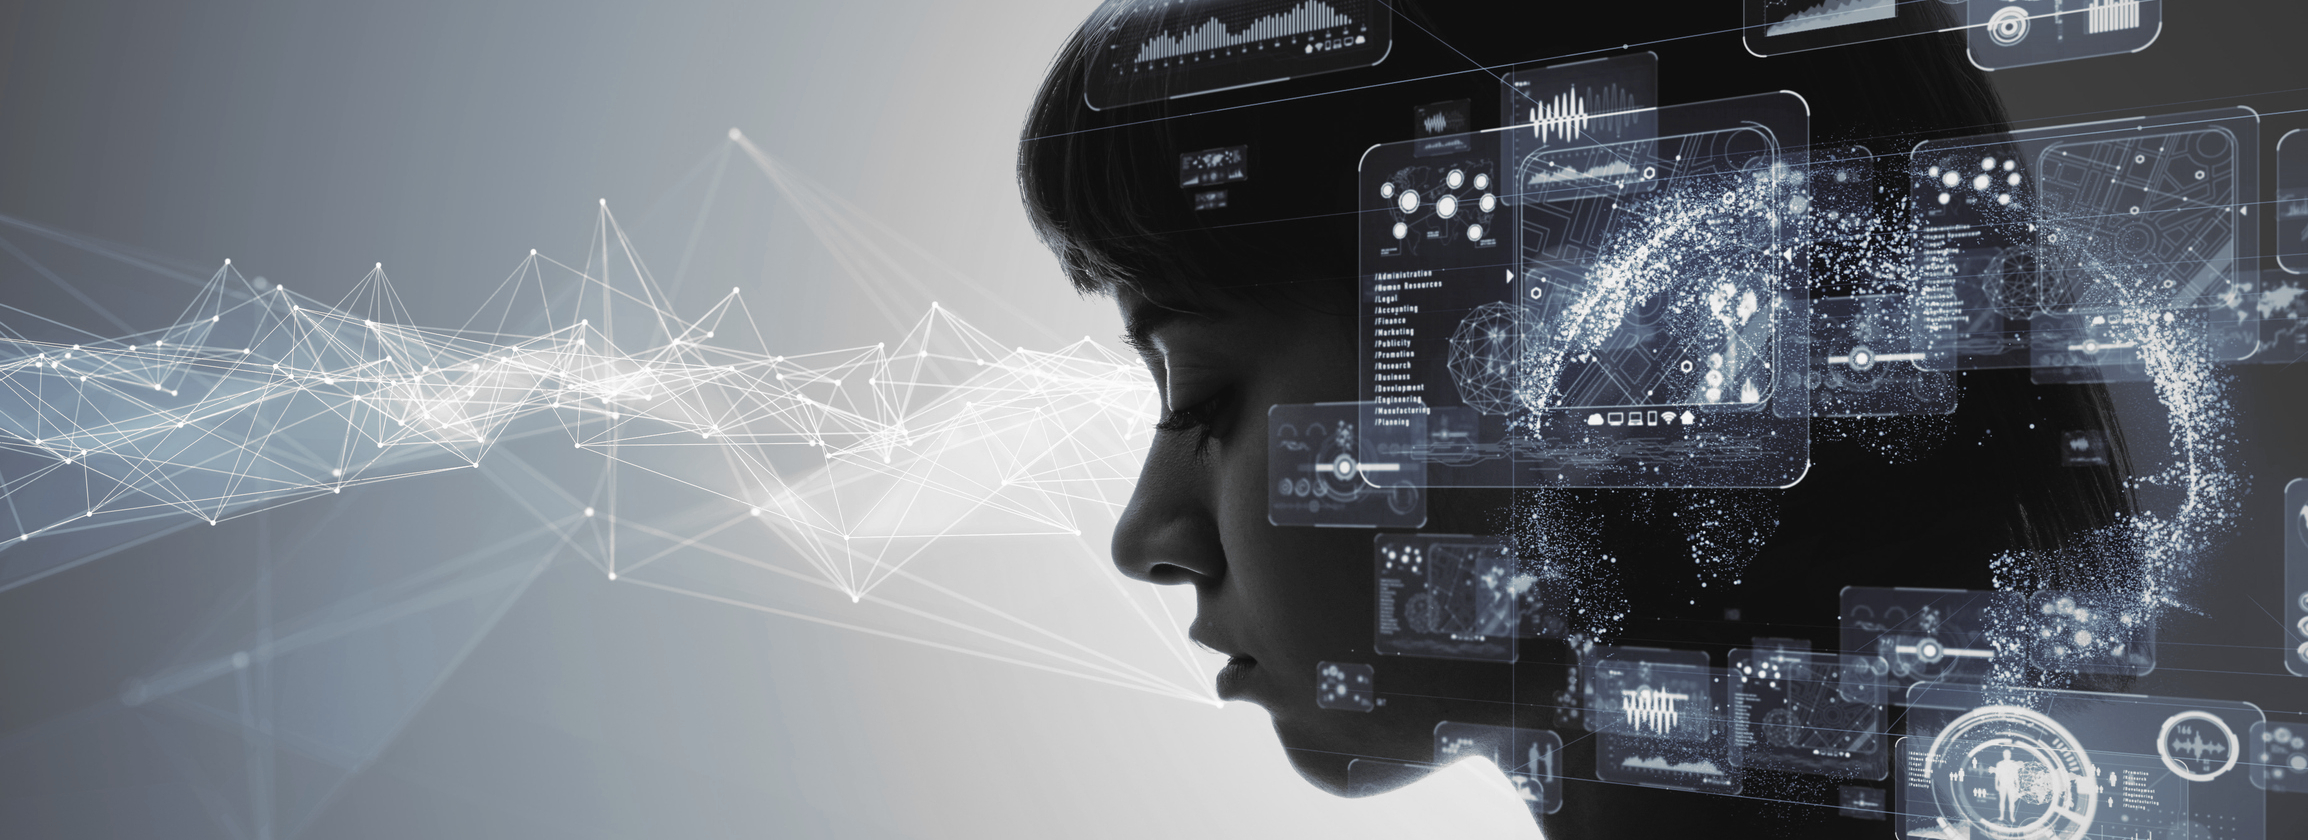
\includegraphics[scale=1]{ai-banner3.jpg}
    \end{center}
    \vfill
    \texttt{Last Update: \today}
}

\begin{document}
\maketitle
This course "COMP2211: Exploring Artificial Intelligence" aims to give a gentle introduction to the basic elements of artificial intelligence (AI) through understanding examples from various applications and hands-on experimentation using AI software tools. In addition to covering the technical aspect of AI through such topics as search and problem solving, knowledge representation, probabilistic reasoning, machine learning, computer vision and image processing, speech and language processing, and robotics, this course will also study the historical perspective, social and ethical implications, as well as potential and limitations of AI.
The following note is made accordingly to the examples and questions of the lecture notes from Professor Desmond TSOI Yau Chat in HKUST. The notes are made to help students understand the course better.
The textbooks used in this course are listed below:
\begin{enumerate}
    \item \textbf{AI Crash Course: A Fun and Hands-On Introduction to Reinforcement Learning, Deep Learning, and Artificial Intelligence with Python} by Hadelin de Ponteves, Kirill Eremenko, and SuperDataScience Team.
    \item \textbf{Python Beginner's Guide to Artificial Intelligence: Build applications to intelligently interact with the world around you using Python} by Denis Rothman, Matthew Lamons, and Rahul Kumar, Abhishek Nagaraja, Amir Ziai, and Ankit Dixit.
    \item \textbf{Artificial Intelligence with Python: Build real-world Artificial Intelligence applications with Python to intelligently interact with the world around you} by Prateek Joshi.
    \item \textbf{Python Image Processing Cookbook: Over 60 recipes to help you perform complex image processing and computer vision tasks with ease} by Sandipan Dey.
\end{enumerate}

\begin{center}
    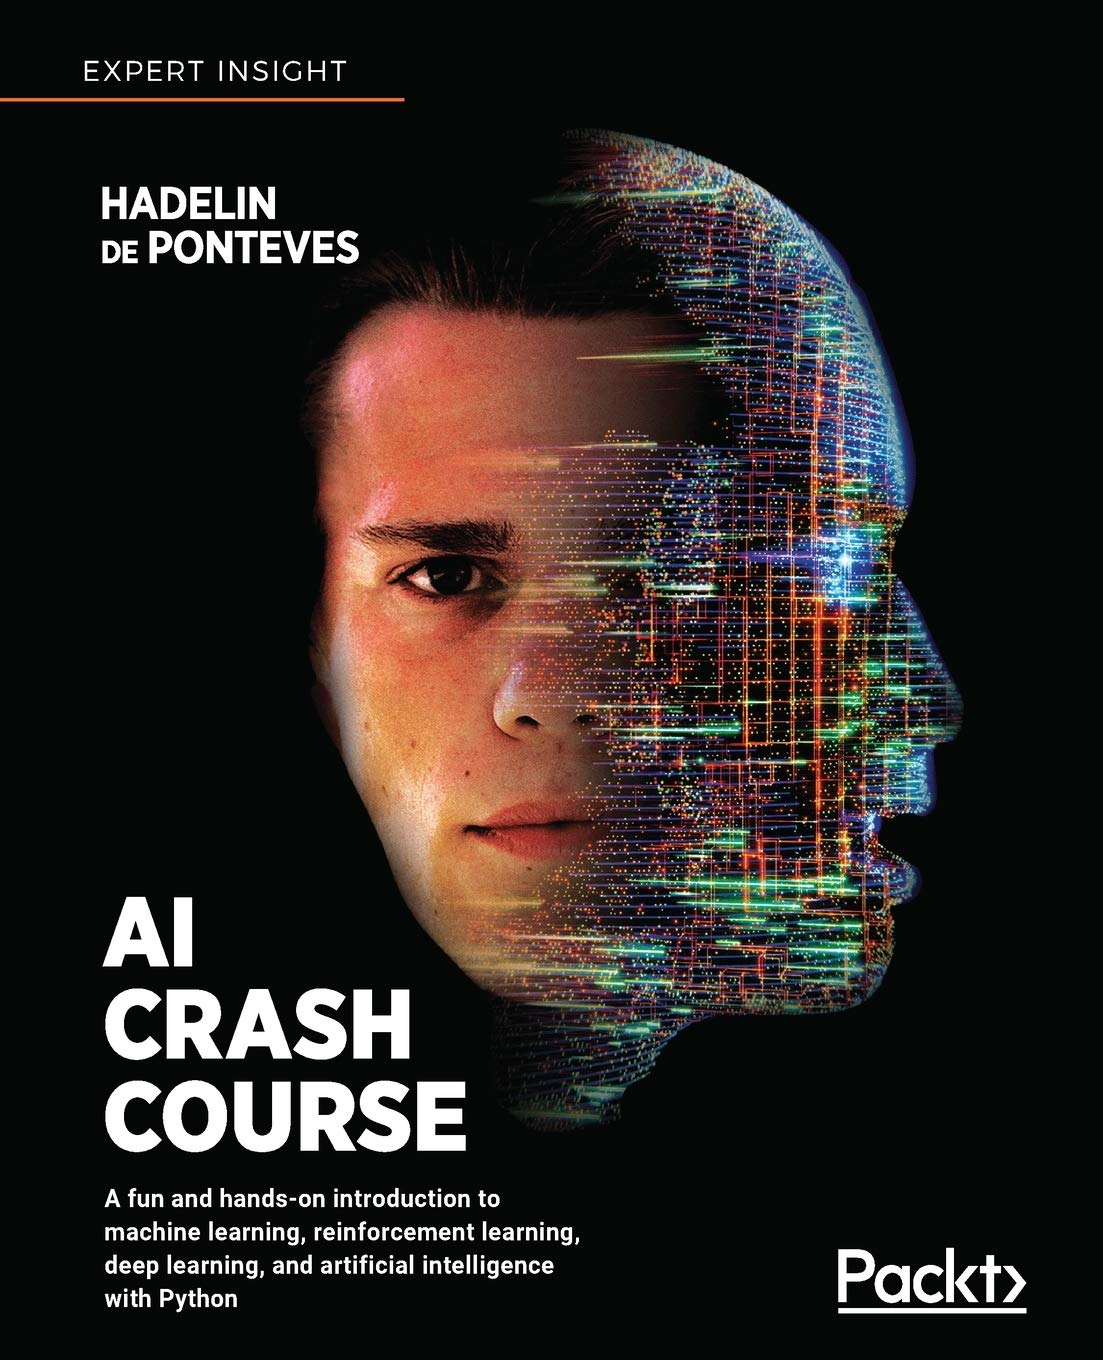
\includegraphics[scale = 0.181]{ai-crash-course.jpg}
    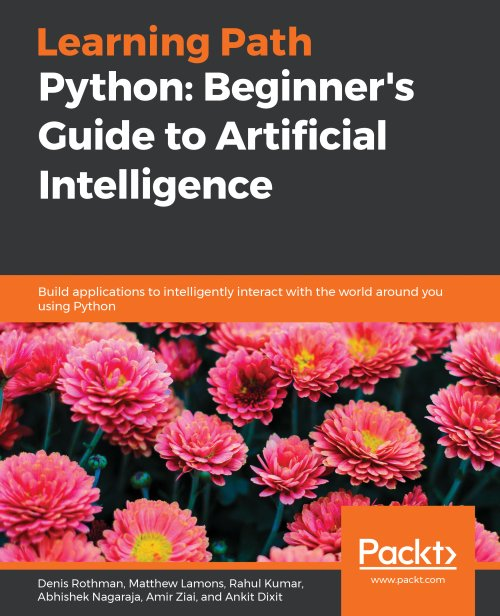
\includegraphics[scale = 0.4]{python-beginner-guide.jpg}
    
\includegraphics[scale = 0.169]{artificial-intelligence-with-python.jpg}
    \includegraphics[scale = 0.09]{ip-cookbook.png}
\end{center}

\tableofcontents
\chapter{Introduction to Artificial Intelligence}
\textcolor{magenta}{\section{\textbf{Definition of Artificial Intelligence}}}
\begin{defBox}[]{Definition 1.1}{Artificial Intelligence}
    \textcolor{cyan}{Artificial Intelligence (AI)} is the \textcolor{red}{science and engineering of making intelligent machines}, espeically intelligent computer programs.
\end{defBox}

AI \textcolor{purple}{borrows characterisitics from human intelligence} and applies them as algorithms in a computer-friendly way.\newline
We study AI due to \textcolor{purple}{Brighter Career for us}, \textcolor{purple}{Skillfulness of AI} and \textcolor{purple}{Skill of the century}.\newline
The terms "Artificial Intelligence", "Machine Learning", "Neural Networks" and "Deep Learning" tend to be used interchangeably in conversation.
\begin{defBox}[]{Definition 1.2}{Machine Learning in AI}
    \textcolor{cyan}{Machine Learning (ML)} is \textcolor{red}{a sub-field of artificial intelligence} that provides systems with the ability to \hl{automatically learn and improve from experience without being explicitly programmed}.\\
    $\Rightarrow$ In ML, there are different algorithms like \textcolor{cyan}{neural networks} that helps to solve problems.
\end{defBox}
\begin{defBox}[]{Definition 1.3}{Deep Learning in ML}
    \textcolor{cyan}{Deep Learning (DL)} is \textcolor{red}{a sub-field of machine learning} and \textcolor{red}{a type of neural networks} to analyze different factors with a structure similar to the human neural system.
\end{defBox}
\begin{figure}[h]
    \centering
    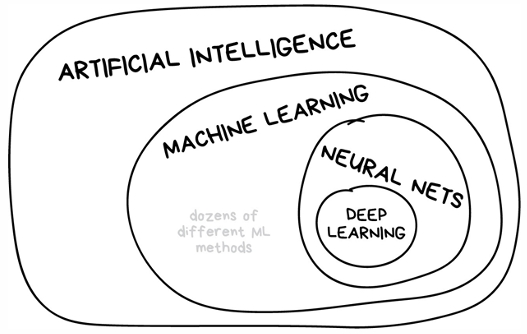
\includegraphics[scale=0.5]{images/Screenshot_20-12-2024_21499_.jpeg}
    \caption{AI, ML and DL}
\end{figure}

\newpage
\textcolor{magenta}{\section{\textbf{Academic Disicplines of AI}}}
AI is a interdisciplinary field that combines the following disciplines:
\begin{description}
    \item[1. Philosophy \& Cognition Science]: Logic, Methods of reasoning, Foundation of Learning, Language, Rationality.
    \item[2. Mathematics]: Write the logic and algorithms for machine. It is must skill to develop  model of AI.
    \item[3. Neuroscience]: \\
    Provide information about how human brain works and how neurons respond to a particular event. Enables AI scienists to develop programming models to work like the human brain.
    \item[4. Psychology]: Study and find the process of thinking of humans and animals.
    \item[5. Computer Science]: Write codes  for making the neural network for AI. 
    \item[6. Linguistics]: Knowledge representation, Grammar.  
\end{description}

\textcolor{magenta}{\section{\textbf{Importance of AI}}}
AI is important because it can help solve immensely complex issues in various industries, such as:
\begin{description}
    \item[1. Gaming \& Entertainiment]: Guides the action of non-human player characters.
    \item[2. Speech Recognition]: Translates speech into text.
    \item[3. Understanding Natural Language]: Carries out dialogue with computers using natural language.
    \item[4. Computer Vision]: Identifies \& Locates objects in digital images \& videos.
    \item[5. Expert Systems]: Emulates the decision-making ability of a human expert.
    \item[6. Healthcare]: Assists diagnosis, Provides telemedicine, Assists surgery using robots, Monitors vital stats.
    \item[7. Air Transport]: Delivers safer air transport while reducing its environmental impact.
    \item[8. Banking \& Financial Institutions]: Automates services and Manages risk.
    \item[9. Logistics]: Delivers goods using autonomous vehicles.
    \item[10. E-commerce]: Personalizes content for customers to boost sales by filtering spam \& fake reviews.
    \item[11. Hiring]: Goes through a lot of CYs \& Ascertains if the candidate is a good fit.          
\end{description}
\textcolor{magenta}{\section{\textbf{Advantages and Disadvantages of AI}}}
There are many advantages and disadvantages of AI.\\
Here are some of the advantages of using AI:
\begin{itemize}
    \item \textcolor{cyan}{Reduction in Human Error}: Computers do not make mistakes if they are programmed properly.
    \item \textcolor{cyan}{Takes Risks instead of Humans}: Overcome many risky limitations of humans by developing an AI Robot which can do the risky things for us.
    \item \textcolor{cyan}{Available 24 hours a day 7 days a week}: Make machines work 24 hours a day 7 days a week without any breaks by using AI and they do not get bored.
    \item \textcolor{cyan}{Digital Assistance}: Use digitial assistants to interact with uses which save the need for human resources (e.g. Siri).
    \item \textcolor{cyan}{Faster Decisions}: Make machines make decisions faster than a human and carry out actions quicker alongside other technologies.
    \item \textcolor{cyan}{New Inventions}: Power many inventions in almost every domain which will help humans solve the majority of complex problems.   
\end{itemize}
\newpage
However, there are also disadvantages of using AI:
\begin{itemize}
    \item \textcolor{cyan}{High Costs of Creation}: \\ Hardware \& Software need to get updated with time to meet the latest requirements. Machines need repairing and maintenance which costs a lot.
    \item \textcolor{cyan}{Making Humans Lazy}: Automates most of the work.
    \item \textcolor{cyan}{Unemployment}: \\ Replace most repetitive tasks and othe works with robots.
    Human interference becomes less whcih cause a major issue in the employment standatds. 
    Companies instead looks to replace the mimimum qualified individuals with AI robots to do similar work with more efficiency.
    \item \textcolor{cyan}{No Emotions}: Bad for Team Management.
    \item \textcolor{cyan}{Lack out of Box Thinking}: \\ Can perform only those tasks designed or programmed to do. Anything out of that tends to crash or give irrelevant outputs, becomes a major backdrop.
\end{itemize}
\textcolor{magenta}{\section{\textbf{History of AI}}}
The history of AI is divided into the following periods:
\begin{itemize}
    \item 1950-1956: The Birth of AI.
    \item 1956-1974: Symbolic AI.
    \item 1974-1980: AI winter.
    \item 1980-1987: Expert Systems.
    \item 1987-1993: AI Winter.
    \item 1993-2011: AI Spring.
    \item 2011-Present: Deep Learning, Big Data, and Artificial General Intelligence.
\end{itemize}
\raggedright
\uline{The Birth of AI (1950-1956)}: \\
\vspace{1mm}
English mathematician \textcolor{cyan}{Alan Turing}, \textcolor{red}{the founder of AI}, introduced the \textcolor{cyan}{Turing Test} in 1950, which is a test to \hl{empirically determine whether a computer has achieved human-level intelligence}.\\
\begin{itemize}
    \item In these tests, one of the human functions as the questioner, while the second human and the computer function as respondents.
    \item The questioner interrogates the respondents within a specific subject area using a specified format and context.
    \item After a preset length of time or number of questions, the questioner tries to determine which respondent is the human and which is the computer.
\end{itemize}
\vspace{1mm}
In 1956, the term "Artificial Intelligence" was coined by John McCarthy at the Dartmouth Conference.\\
\vspace{1mm}
\uline{Symbolic AI (1956-1974)}: \\
\vspace{1mm}
In 1959, Arthur Samuel coined the term "Machine Learning" and developed the first self-learning program, which played checkers.\\
In 1965, Joseph Weizenbaum developed ELIZA, an early natural language processing computer program.\\
\vspace{1mm}
\uline{Expert Systems (1980-1987)}: \\
\vspace{1mm}
In the 1980s, expert systems were developed by Edward Feigenbaum, which were the first commercial AI systems.\\
\vspace{1mm}
\uline{AI Spring (1993-2011)}: \\
\vspace{1mm}
In the 1990s, Cynthia Breazeal developed Kismet, a robot that could recognize and simulate human emotions.\\
In 1997, IBM's Deep Blue defeated the world chess champion, Garry Kasparov.\\
iRobot's Roomba, a vacuum cleaning robot, was introduced in 2002.\\
The first self-driving car was developed by Google to handle urban environments in 2009.\\
IBM's Watson defeated the world Jeopardy champion in 2011.\\
\vspace{1mm}
\uline{Deep Learning, Big Data, and Artificial General Intelligence (2011-Present)}: \\
\vspace{1mm}
Personal assistants like Apple's Siri, Amazon's Alexa, and Google Assistant were introduced.\\
Ian Goodfellow introduced Generative Adversarial Networks (GANs) in 2014.\\
In 2016, Google's AlphaGo defeated the world Go champion.\\
In 2022, OpenAI's ChatGPT was released, which is a language model that can generate human-like text.\\
Bard, an experimental conservational AI chat service, was developed by Google in 2023.\\
\newpage
\textcolor{magenta}{\section{\textbf{Useful AI and Machine Learning Libraries}}}
There are 4 main libraries that are used in AI and Machine Learning:
\begin{itemize}
    \item \textcolor{cyan}{\texttt{TensorFlow}}: An open-source machine learning library developed by Google, which is fast, flexible, and scalable for research and production.
    \item \textcolor{cyan}{\texttt{Keras}}: A high-level application programming interface (API) built on top of TensorFlow, which is user-friendly, fast experimentation, and easy to pick up.
    \item \textcolor{cyan}{\texttt{PyTorch}}: An open-source machine learning library developed by Facebook to compete with TensorFlow, allowing unlimited customization and flexibility.
    \item \textcolor{cyan}{\texttt{Scikit-learn}}: A User-Friendly Framework for Python with a lot of useful tools including classification, regression, clustering, dimensionality reduction, model selection, and preprocessing.
\end{itemize}
\uline{Comparison between TensorFlow and PyTorch}: \\
\vspace{1mm}
\textcolor{cyan}{TensorFlow} has a difficult learning curve with good documentations and lots of examples, while \\
\textcolor{cyan}{PyTorch} has a slightly simplier learning curve with weak and skimpy documentation.\\
\vspace{1mm}
$\therefore$ We use \textcolor{cyan}{Scikit-learn} and \textcolor{cyan}{Keras} for beginners in AI and Machine Learning since they are \textcolor{red}{easier to use} and \textcolor{red}{have a simpliest learning curve (less flexible)}.
\begin{center}
    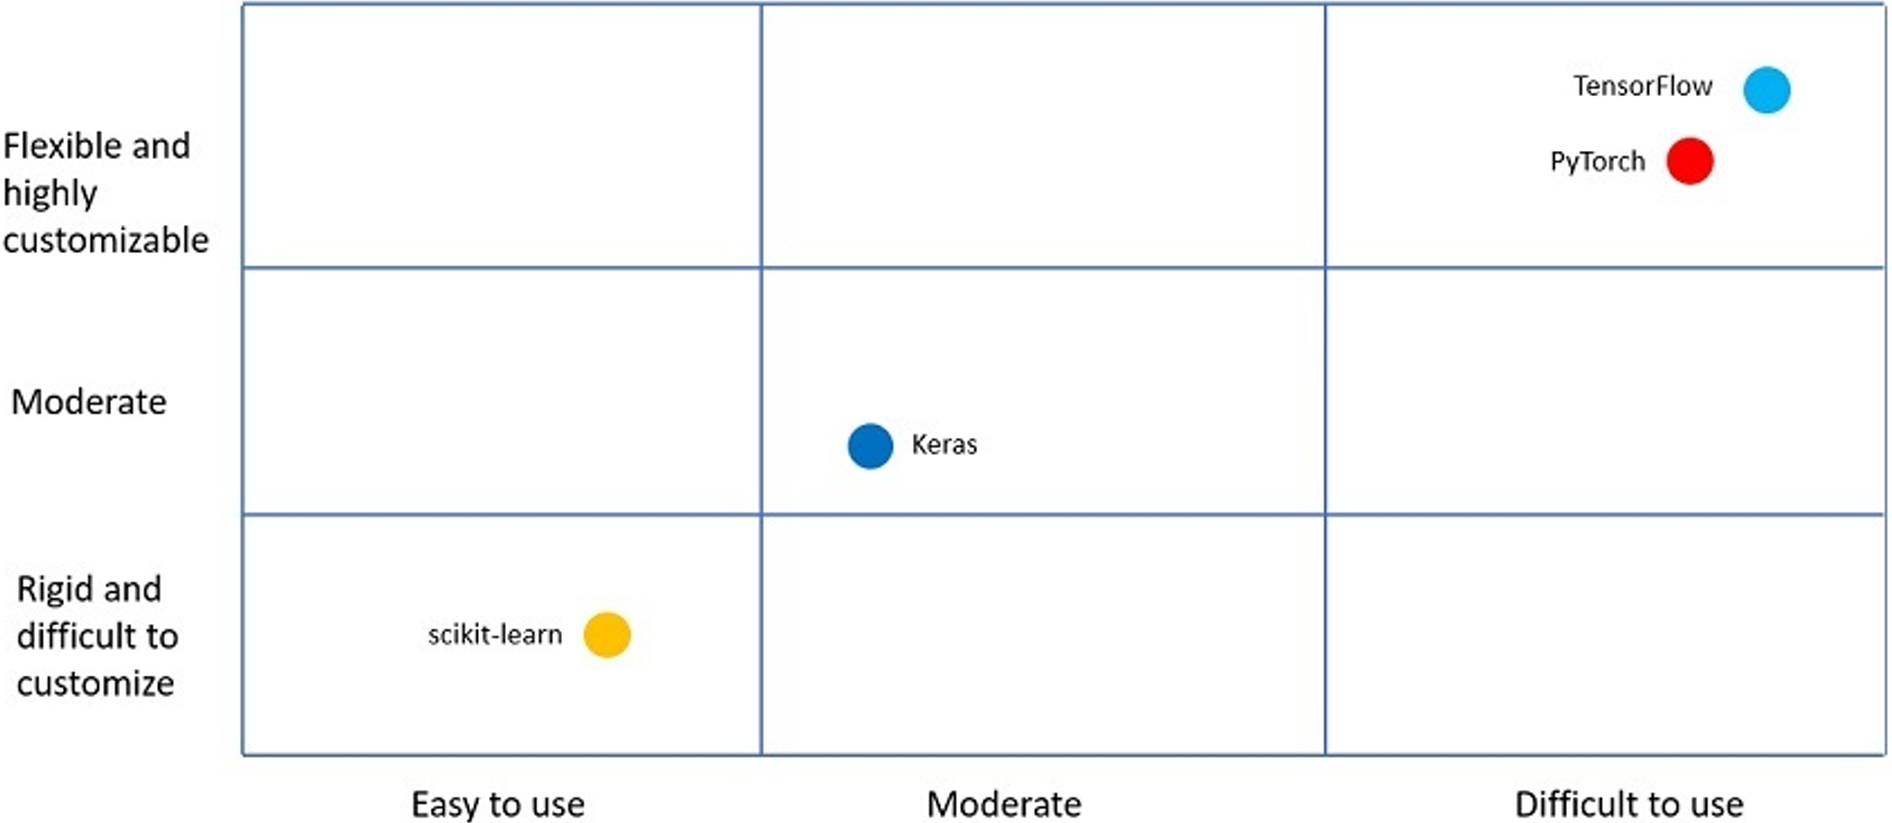
\includegraphics[scale=0.2]{tensorflow_vs_pytorch.jpeg}
\end{center}
\textcolor{magenta}{\section{\textbf{Advantages and Disadvantages of Using Python for AI}}}
Python is a popular programming language for AI. There are some of the advantages and disadvantages of using Python for AI.\\
Here are some of the advantages of using Python for AI:
\begin{itemize}
    \item Relatively easy to learn \& read compared to other programming languages.
    \item Lots of Machine Learning Libraries and Useful Tools.
    \item Popular among Data Scientists.
    \item Many useful machine-learning repositories.
    \item Easy to integrate with other programming languages.
\end{itemize}
However, there are also disadvantages of using Python for AI:
\begin{itemize}
    \item Speed limitations (Use vectorization instead of loops).
    \item Not suitable for mobile \& game development.
    \item Design limitations.
\end{itemize}
\chapter{Advanced Python for Artificial Intelligence}
\textcolor{magenta}{\section{\textbf{Crash Course on More Advanced Python Programming Elements}}}
    \subsection{Data Types ad type Function}
    Python has a number of basic types including \textcolor{cyan}{integers, floats, booleans, strings and containers (lists, dictionaries, sets, tuples)}.\\
    \textcolor{cyan}{\texttt{type()}} function \textcolor{violet}{returns class type of the object} passed as parameter, mostly used for debugging.
    \begin{synBox}[]{Syntax 2.1}{\texttt{type()}}
        \begin{lstlisting}[language=Python, basicstyle=\ttfamily\small, keywordstyle=\color{blue}, commentstyle=\color{forestgreen}, stringstyle=\color{red}, showstringspaces=false]
                                        type(object)
        \end{lstlisting}
    \end{synBox}
    \begin{egBox}[]{Example 2.1.1}{}
        \begin{lstlisting}[language=Python, basicstyle=\ttfamily\small, keywordstyle=\color{blue}, commentstyle=\color{forestgreen}, stringstyle=\color{red}, showstringspaces=false]
                            x = 3                   # <class 'int'>
                            y = 3.14                # <class 'float'>
                            z = True                # <class 'bool'>
                            str = "Hello"           # <class 'str'>
                            l = [1, 2, 3]           # <class 'list'>
                            d = {"a": 1, "b": 2}    # <class 'dict'>
                            s = {1, 2, 3}           # <class 'set'>
                            t = (1, 2, 3)           # <class 'tuple'>
        \end{lstlisting}
    \end{egBox}
    \subsection{List Comprehensions}
    List comprehensions offer a \textcolor{violet}{shorter syntax} when we want to \textcolor{violet}{create a new list based on the values of an existing list}. \\ 
    List comprehensions start and end with opening and closing \texttt{[]} brackets repsectively. \\
    There can be an optional if statement and additional for clause.
    \begin{synBox}[]{Syntax 2.2}{List Comprehensions}
    \begin{lstlisting}[language=Python, basicstyle=\ttfamily\small, keywordstyle=\color{blue}, commentstyle=\color{forestgreen}, stringstyle=\color{red}, showstringspaces=false]
                new-list-name = [expression for item in list-name if condition]
    \end{lstlisting}
        \raggedright
        where: \\
        \begin{description}
            \item[$\bullet$] \textcolor{brown}{\texttt{expression}}: Operation we perform on each value inside the original list.
            \item[$\bullet$] \textcolor{brown}{\texttt{element}}: Temporary variable we use to store for each item in the original list.
            \item[$\bullet$] \textcolor{brown}{\texttt{list-name}}: Name of the list we want to go through.
            \item[$\bullet$] \textcolor{brown}{\texttt{condition}}: If \texttt{condition} == True, add the processed element to the new list.
            \item[$\bullet$] \textcolor{brown}{\texttt{new-list-name}}: New values created which are saved.
        \end{description}
    \end{synBox}
    \newpage
    \begin{egBox}[]{Example 2.1.2}{}
    \begin{lstlisting}[language=Python, basicstyle=\ttfamily\small, keywordstyle=\color{blue}, commentstyle=\color{forestgreen}, stringstyle=\color{red}, showstringspaces=false]
    numbers = [0, 1, 2, 3, 4]
    squares = [number **2 for number in numbers] # [0, 1, 4, 9, 16]
    even_squares = [number **2 for number in numbers if number % 2 == 0] # [0, 4, 16]
    \end{lstlisting}
    \end{egBox}
    \subsection{Dictionary Comprehensions}
    Dictionary comprehensions offer a \textcolor{violet}{shorter syntax} when we want to \textcolor{violet}{create a new dictionary based on the values of an existing dictionary}. \\
    Dictionary comprehensions start and end with opening and closing \{ \} brackets respectively. \\
    It is similar to list comprehensions but with a key-value pair.
    \begin{egBox}[]{Example 2.1.3}{}
    \begin{lstlisting}[language=Python, basicstyle=\ttfamily\small, keywordstyle=\color{blue}, commentstyle=\color{forestgreen}, stringstyle=\color{red}, showstringspaces=false]
    numbers = [0, 1, 2, 3, 4]
    
    # {0: 0, 2: 4, 4: 16}
    even_num_to_square = {number: nummber **2 for number in numbers if number % 2 == 0} 
    \end{lstlisting}
    \end{egBox}
    \subsection{Set Comprehensions}
    Set comprehensions offer a \textcolor{violet}{shorter syntax} when we want to \textcolor{violet}{create a new set based on the values of an existing set}. \\
    Set comprehensions start and end with opening and closing \{ \} brackets respectively. \\
    It is similar to list comprehensions and dictionary comprehensions but with a set.
    \begin{egBox}[]{Example 2.1.4}{}
    \begin{lstlisting}[language=Python, basicstyle=\ttfamily\small, keywordstyle=\color{blue}, commentstyle=\color{forestgreen}, stringstyle=\color{red}, showstringspaces=false]
        from math import sqrt
        numbers = {int(sqrt(number)) for number in range(30)} # {0, 1, 2, 3, 4, 5}
    \end{lstlisting}
    \end{egBox}
    \subsection{Tuples}
    \textcolor{cyan}{Tuples} can be \textcolor{violet}{used as keys in dictionaries and as elements of sets}, while lists cannot.
    \begin{egBox}[]{Example 2.1.5}{}
    \begin{lstlisting}[language=Python, basicstyle=\ttfamily\small, keywordstyle=\color{blue}, commentstyle=\color{forestgreen}, stringstyle=\color{red}, showstringspaces=false]
                    # Create a dictionary with tuple keys
                    d = {(x, x + 1): x for x in range(10)}
                    t = (5, 6)          # Create a tuple
                    print(type(t))      # <class 'tuple'>
                    print(d[t])         # 5
                    print(d[(1, 2)])    # 1
                    
                    # Error of Tuples
                    l = [1, 2]
                    print(type(l))      # <class 'list'>
                    print(d[l])         # TypeError: unhashable type: 'list'
    \end{lstlisting}
    \end{egBox}
    \newpage
    \subsection{Parallel Iteration}
    \textcolor{cyan}{\texttt{zip()} method} \textcolor{violet}{take iterable or containers} and \textcolor{violet}{return a single interator object, having mapped values} from all containers.
    If the passed iterable or containers have \textcolor{violet}{different length}, the one with \hl{the least items decides the length of the new iterator}.
    \begin{synBox}{Syntax 2.3}{\texttt{zip()}}
        \begin{lstlisting}[language=Python, basicstyle=\ttfamily\small, keywordstyle=\color{blue}, commentstyle=\color{forestgreen}, stringstyle=\color{red}, showstringspaces=false]
                            zip(iterable1, iterable2, iterable3, ...)
        \end{lstlisting}
        \raggedright
        where: \\
        \begin{description}
            \item[$\bullet$] \textcolor{brown}{\texttt{iterable1, iterable2, iterable3, ...}}: Iterator objects that will be joined together.
        \end{description}
    \end{synBox}
    \begin{egBox}[]{Example 2.1.6}{}
    \begin{lstlisting}[language=Python, basicstyle=\ttfamily\small, keywordstyle=\color{blue}, commentstyle=\color{forestgreen}, stringstyle=\color{red}, showstringspaces=false]
                        characters = ['A', 'B', 'C']
                        numbers = ['1', '2', '3']
                        for character, number in zip(characters, numbers):
                            print(f'{character} is {number}')
                        # A is 1
                        # B is 2
                        # C is 3
    \end{lstlisting}
    \end{egBox}
    \subsection{Functions}
    If we \textcolor{violet}{do not know how many arguments} that will be passed into our function, \textcolor{violet}{add an asterisk (*) before the paramter name} in the function definition.\\
    The function will receive a tuple of arguments and can access the items accordingly.
    \begin{egBox}[]{Example 2.1.7.1}{}
    \begin{lstlisting}[language=Python, basicstyle=\ttfamily\small, keywordstyle=\color{blue}, commentstyle=\color{forestgreen}, stringstyle=\color{red}, showstringspaces=false]
                        def print_kids(*kids):
                            print('The youngest child is ' + kids[2])
                        print_kids('A', 'B', 'C')
                        # The youngest child is C
    \end{lstlisting}
    \end{egBox}
    If we \textcolor{violet}{do not know how many keyword arguments} that will be passed into our function, \textcolor{violet}{add two asterisks (**) before the parameter name} in the function definition. \\
    The function will receive a dictionary of arguments and can access the items accordingly:
    \begin{egBox}[]{Example 2.1.7.2}{}
    \begin{lstlisting}[language=Python, basicstyle=\ttfamily\small, keywordstyle=\color{blue}, commentstyle=\color{forestgreen}, stringstyle=\color{red}, showstringspaces=false]
def print_kids(**kids):
  print('The youngest child is ' + kids['kid3'] + 'and the oldest child is ' + kids['kid1'])
# The youngest child is C and the oldest child is A.
print_kids(kid1='A', kid2='B', kid3='C')
    \end{lstlisting}
    \end{egBox}
    \subsection{Object-Oriented Programming and Classes}
    \textcolor{cyan}{Object-Oriented Programming (OOP)} is a way of structuring a program by \textcolor{violet}{bundling related properties (data) and behaviors (functionality)} into individual objects. \\
    $\Rightarrow$ Five Features of OOP: \textcolor{red}{Classes}, \textcolor{red}{Objects}, \textcolor{red}{Inheritance}, \textcolor{red}{Polymorphism} and \textcolor{red}{Dynamic Binding}.\\
    The fundamental concepts of OOP can be introduced via the use of \textcolor{cyan}{classes} and \textcolor{cyan}{objects}.
    \newpage
    \textcolor{olive}{\subsubsection{Definition of Classes}}
    \textcolor{cyan}{Classes} are \hl{user-defined data types} from which objects are created. They are created by \textcolor{violet}{keyword classes}.\\
    Class provides a means of \hl{bundling data (instance variables)} and \hl{functionality(methods)} together.\\
    Instance Variables:
    \begin{description}
        \item[$\bullet$] Variables that belong to an object.
        \item[$\bullet$] \textcolor{violet}{Always public by default} and can be \textcolor{violet}{accessed using the dot(.) operator}.
    \end{description}
    Methods:
    \begin{description}
        \item[$\bullet$] Have an extra \textcolor{violet}{first parameter self} in the method definition.
        \item[$\bullet$] \textcolor{violet}{Do not give a value for this parameter} when we call the method.
    \end{description}
    The \textcolor{cyan}{\texttt{\_\_init\_\_} method} is used as \hl{constructor} to \textcolor{violet}{initialize the instance variables of objects}.
    \begin{synBox}[]{Syntax 2.4}{Class with Instance Variables, Methods and Constructor}
        \begin{lstlisting}[language=Python, basicstyle=\ttfamily\small, keywordstyle=\color{blue}, commentstyle=\color{forestgreen}, stringstyle=\color{red}, showstringspaces=false]
                        class ClassName:
                            # __init__ is a constructor
                            def __init__(self, argument0):
                                self.instance_variable1 = value1
                                self.instance_variable2 = value2
                                ...

                            # Methods
                            def method1_name(self, argument1):
                                statement1
                                statement2
                                ...
                            def method2_name(self, argument2):
                                statement1
                                statement2
                                ...
        \end{lstlisting} 
    \raggedright
    where: \\
    \begin{description}
        \item[$\bullet$] \texttt{\textcolor{brown}{ClassName}}: Name of the class.
        \item[$\bullet$] \texttt{\textcolor{brown}{argument0, argument1, argument2, ...}}: Method Parameters (Variables)
        \item[$\bullet$] \texttt{\textcolor{brown}{instance\_variable1, instance\_variable2, ...}}: Instance Variables.
        \item[$\bullet$] \texttt{\textcolor{brown}{value1, value2, ...}}: Values assigned to the instance variables.
        \item[$\bullet$] \texttt{\textcolor{brown}{statement1, statement2, ...}}: Python statements.
    \end{description}
    \end{synBox}
    \begin{synBox}{Syntax 2.5}{Creating Objects, Calling Methods and Modfying Instance Variables}
        \begin{lstlisting}[language=Python, basicstyle=\ttfamily\small, keywordstyle=\color{blue}, commentstyle=\color{forestgreen}, stringstyle=\color{red}, showstringspaces=false]   
            object_name = ClassName(arguments)          # Create an object.          
            object_name.method_name(arguments)          # Call a method.          
            object_name.instance_variable_name = value  # Modify an instance variable.
        \end{lstlisting}
    \raggedright
    where: \\
    \begin{description}
        \item[$\bullet$] \texttt{\textcolor{brown}{object\_name}}: Name of the object.
        \item[$\bullet$] \texttt{\textcolor{brown}{ClassName}}: Name of the class.
        \item[$\bullet$] \texttt{\textcolor{brown}{arguments}}: Values passed to the constructor/method.
        \item[$\bullet$] \texttt{\textcolor{brown}{method\_name}}: Name of the method.
        \item[$\bullet$] \texttt{\textcolor{brown}{instance\_variable\_name}}: Name of the instance variable.
        \item[$\bullet$] \texttt{\textcolor{brown}{value}}: Value assigned to the instance variable.
    \end{description}
    \end{synBox}
    \newpage
    \begin{egBox}[]{Example 2.1.8.1}{}
    \begin{lstlisting}[language=Python, basicstyle=\ttfamily\small, keywordstyle=\color{blue}, commentstyle=\color{forestgreen}, stringstyle=\color{red}, showstringspaces=false]
import math                                 # Import math library

class Circle:                               # Define a class
    def __init__(self, radius):             # Constructor
        self.radius = radius                # Instance variable

    def area(self):                         # Method
        return math.pi * self.radius ** 2   # Calculate area

    def circumference(self):                # Method
        return 2 * math.pi * self.radius    # Calculate circumference

circle = Circle(3)                          # Create an object named circle with radius 3.
circle.radius = 4                           # Modify the instance variable radius to 4.
print(circle.area())                        # Call the area method.
print(circle.circumference())               # Call the circumference method.
    \end{lstlisting}
    \end{egBox}
    \textcolor{olive}{\subsubsection{Public, Private and Protected Data Members}}
    \raggedright All members in a Python class are \textcolor{violet}{public by default}, meaning \textcolor{violet}{any member can be accessed from outside the class}.\\
    We make some members protected/private to restrict the access to these members.\\
    \begin{description}
        \item[$\bullet$] \textcolor{cyan}{Protected Data Members}:\\
        Protected members of a class are \textcolor{violet}{accessible from within the class and also available to its sub-classes}.\\
        To define a protected member, \textcolor{violet}{prefix the instance variable/method name with a single underscore (\_)}.
        \item[$\bullet$] \textcolor{cyan}{Private Data Members}:\\
        Private members of a class are \textcolor{violet}{accessible only within the class}.\\
        To define a private member, \textcolor{violet}{prefix the instance variable/method name with two underscores (\_\_)}.
    \end{description}
    \textcolor{red}{Error} with Accessing Private Instance Variables Outside Class:
    \begin{egBox}[]{Example 2.1.8.2}{}
    \begin{lstlisting}[language=Python, basicstyle=\ttfamily\small, keywordstyle=\color{blue}, commentstyle=\color{forestgreen}, stringstyle=\color{red}, showstringspaces=false]
    class Person:
        def __init__(self, name = "Tom", age=18, gender='M'):
            self.__name = name              # Private Instance Variable __name
            self.__age = age                # Private Instance Variable __age
            self.__gender = gender          # Private Instance Variable __gender
    
    desmond = Person('Desmond', 1000, 'M')
    print('Name: ' + desmond.__name)        # Error
    print('Age: ' + str(desmond.__age))     # Error
    print('Gender: ' + desmond.__gender)    # Error

    desmond.__name = 'Desmond TSOI'         # No Error, but does not change desmond.__name.
    desmond.__age = -10                     # No Error, but does not change desmond.__age.
    \end{lstlisting}
    \end{egBox}
    To \textcolor{violet}{retrieve and modify instance variable values}, we need to define \textcolor{orange}{accessors and mutators}.
    \newpage
    \textcolor{olive}{\subsubsection{Accessors and Mutators}}
    Accessor and Mutator Methods are used to \textcolor{violet}{access the protected/private instance variables} which cannot be accessed  from outside the class.
    \begin{description}
        \item[$\bullet$] \textcolor{cyan}{Accessors/Getters}:\\
        Accessor methods are used to \textcolor{violet}{retrieve the values of instance variables of the object}.\\
        When the accessor method is called, it returns the private instance variable value of the object.
        \item[$\bullet$] \textcolor{cyan}{Mutators/Setters}:\\
        Mutator methods are used to \textcolor{violet}{modify the values of instance variables of the object}.\\
        When the mutator method is called, it modifies the private instance variable value of the object.
    \end{description}
    \textcolor{red}{No Errors} by Adding Accessors and Mutators:
    \begin{egBox}[]{Example 2.1.8.3}{}
    \begin{lstlisting}[language=Python, basicstyle=\ttfamily\small, keywordstyle=\color{blue}, commentstyle=\color{forestgreen}, stringstyle=\color{red}, showstringspaces=false]
class Person:
    def __init__(self, name = 'Tom', age=18, gender='M')
        self.__name = name
        self.__age = age
        self.__gender = gender

    def get_name(self):             # Accessor
        return self.__name
    def get_age(self):              # Accessor
        return self.__age
    def get_gender(self):           # Accessor
        return self.__gender
    def set_name(self, name):       # Mutator
        self.__name = name
    def set_age(self, age):         # Mutator
        self.__age = age
    def set_gender(self, gender):   # Mutator
        self.__gender = gender
    
desmond = Person('Desmond', 1000, 'M')
print('Name: ' + desmond.get_name())        # Desmond (No Error).
print('Age: ' + str(desmond.get_age()))     # 1000 (No Error).
print('Gender: ' + desmond.get_gender())    # M (No Error).

desmond.set_name('D TSOI')                  # No Error, changes desmond.__name to 'D TSOI'.
desmond.set_age(-10)                        # No Error, changes desmond.__age to -10.
    \end{lstlisting}
    \end{egBox}
    \textcolor{olive}{\subsubsection{Class Variables}}
    \textcolor{cyan}{Class Variables} are variables \textcolor{violet}{defined within a class and outside of any method}.\\
    They are \hl{shared by all instances of the class}: If the variable's value is changed, it will be changed for all instances of the class.\\
    There are \hl{only one copy of the class variable} and when any object makes a change to a class variable, the change will be reflected in all other objects as well.\\
    They can be \textcolor{violet}{accessed using the class name} followed by the class variable name:
    \begin{lstlisting}[language=Python, basicstyle=\ttfamily\small, keywordstyle=\color{blue}, commentstyle=\color{forestgreen}, stringstyle=\color{red}, showstringspaces=false]
                                    ClassName.class_variable
    \end{lstlisting}
    \newpage
    \begin{egBox}[]{Example 2.1.8.4}{}
    \begin{lstlisting}[language=Python, basicstyle=\ttfamily\small, keywordstyle=\color{blue}, commentstyle=\color{forestgreen}, stringstyle=\color{red}, showstringspaces=false]
                    class Person:
                        num_person = 0              # Class Variable
                        def __init__(self, name='Tom', age=18, gender='M'):
                            self.__name = name
                            self.__age = age
                            self.__gender = gender
                            Person.num_person += 1
                        
                    desmond = Person('Desmond', 1000, 'M')
                    pearl = Person('Pearl', 1000, 'F')
                    print(Person.num_person)        # 2
    \end{lstlisting}
    \end{egBox}
    \small Comparison between \textcolor{blue}{Class Variables} and \textcolor{blue}{Instance Variables}:
    \begin{center}
        \begin{tabular}{|m{2.1cm}|m{8.5cm}|m{8.5cm}|}
            \hline
            \rowcolor{lightblue}
            & \textbf{Class Variables} & \textbf{Instance Variables} \\
            \hline
            \textbf{Definition} & Defined within the class but outside of any methods. & Defined within methods, typically the constructor. \\
            \hline
            \textbf{Scope} & Changes made to the class variables affect all instances & Changes made to the instance variables do not affect all instances. \\
            \hline
            \textbf{Initialization} & Initialized inside or outside the class definition. & Typically initialized in the constructor. \\
            \hline
            \textbf{Access} & Accessed using the class name followed by the class variable name. & Accessed using the instance name followed by the instance variable name. \\
            \hline
            \textbf{Usage} & Used for storing data that is shared among all instances of the class like constants and default values. & Used for storing data that is unique to each instance of the class like the object properties. \\
            \hline
        \end{tabular}
    \end{center}
    \textcolor{olive}{\subsubsection{Inheritance}}
    \textcolor{cyan}{Inheritance} is a mechanism that allows us to \textcolor{violet}{define a new class based on existing classes}.\\
    All the \textcolor{violet}{attributes and methods} of existing classes \textcolor{violet}{will be inherited} by the new class.
    \begin{description}
        \item[$\bullet$] \textcolor{cyan}{Existing Classes} = \textcolor{violet}{Parent/Super/Base Classes}.
        \item[$\bullet$] \textcolor{cyan}{New Class} = \textcolor{violet}{Child/Sub/Derived Classes}.
    \end{description}
    \begin{synBox}{Syntax 2.6}{Inheritance}
        \begin{lstlisting}[language=Python, basicstyle=\ttfamily\small, keywordstyle=\color{blue}, commentstyle=\color{forestgreen}, stringstyle=\color{red}, showstringspaces=false]
    class SubClassName(ParentClass1, ParentClass2, ...):

        # __init__ is a constructor.
        def __init__(self, argument0):
            super().__init__(attributes)        # Call the constructor of the parent class.
            self.instance_variable1 = value1
            self.instance_variable2 = value2
            ...
        
        # Methods
        def method1_name(self, argument1):
            statement1
            statement2
            ...
        \end{lstlisting}
    \raggedright
    where: \\
    \begin{description}
        \item[$\bullet$] \texttt{\textcolor{brown}{SubClassName}}: Name of the subclass.
         \item[$\bullet$] \texttt{\textcolor{brown}{ParentClass1, ParentClass2, ...}}: Name of the parent classes.
         \item[$\bullet$] \texttt{\textcolor{brown}{argument0, argument1}}: Method Parameters (Variables).
         \item[$\bullet$] \texttt{\textcolor{brown}{instance\_variable1, instance\_variable2, ...}}: Instance Variables.
         \item[$\bullet$] \texttt{\textcolor{brown}{value1, value2, ...}}: Values assigned to the instance variables.
         \item[$\bullet$] \texttt{\textcolor{brown}{statement1, statement2, ...}}: Python statements.
    \end{description}
    \end{synBox}
    \newpage
    \begin{egBox}[]{Example 2.1.8.5}{}
    \begin{lstlisting}[language=Python, basicstyle=\ttfamily\small, keywordstyle=\color{blue}, commentstyle=\color{forestgreen}, stringstyle=\color{red}, showstringspaces=false]
class Person:
    def __init__(self, name = 'Tom', age=18, gender='M')
        self.__name = name
        self.__age = age
        self.__gender = gender
    def get_name(self):             # Accessor
        return self.__name
    def get_age(self):              # Accessor
        return self.__age
    def get_gender(self):           # Accessor
        return self.__gender
    def set_name(self, name):       # Mutator
        self.__name = name
    def set_age(self, age):         # Mutator
        self.__age = age
    def set_gender(self, gender):   # Mutator
        self.__gender = gender
    def print(self):
        print('Name: ' + self.__name)
        print('Age: ' + str(self.__age))
        print('Gender: ' + self.__gender)

# Define a new type Student that inherits Person class.
class Student(Person):
    def __init__(self, name = 'Tom', age=18, gender='M', id="12345678"): # Constructor
        super().__init__(name, age, gende) # Invoke parent class constructor.
        self.__id = id             # Define instance variable id & assign it with parameter.

    def get_id(self): return self.__id     # Accessor
    def set_id(self, id): self.__id = id   # Mutator

    def print(self):                       # Override print method of the parent class.
        super().print()                    # Invoke print method of the parent class.
        print('ID: ' + self.__id)          # Print ID.

desmond = Student('Desmond', 1000, 'M', '12345678') # Create an object named desmond.
desmond.print()                                     # Print desmond

# Output:

# Name: Desmond
# Age: 1000
# Gender: M
# ID: 12345678
    \end{lstlisting}
    \end{egBox}
\textcolor{magenta}{\section{\textbf{Other Essentials for Writing AI Programs}}}
\subsection{Modules, Packages, Libraries}
\begin{defBox}{Definition 2.1}{Modules}
    A \textcolor{cyan}{module} in Python is a bunch of \textcolor{red}{related code (functions, classes, variables) saved in a file} with the extension .py.
\end{defBox}
\begin{defBox}{Definition 2.2}{Packages}
    A \textcolor{cyan}{package} is a \textcolor{red}{directory of a collection of modules}.
\end{defBox}
\begin{defBox}{Definition 2.3}{Libraries}
    A \textcolor{cyan}{library} is a \textcolor{red}{collection of packages}.
\end{defBox}
\newpage
\subsection{Imports}
The \textcolor{cyan}{"\texttt{import}" keyword} is the most common way to \textcolor{violet}{access external modules}.\\
Modules can be referenced in our program without the need to write them ourselves.\\
We can get access to machine learning libraries like \textcolor{violet}{NumPy, Pandas, Matplotlib, Scikit-Learn} by importing them, similar to the \#include directive in C++.\\
However, since we \textcolor{violet}{usually do not need the entire module}, we can use the \textcolor{cyan}{"\texttt{from}" keyword} to \textcolor{violet}{import only the exact functions/classes/variables} we need.\\
\begin{synBox}{Syntax 2.7}{Imports}
    \begin{lstlisting}[language=Python, basicstyle=\ttfamily\small, keywordstyle=\color{blue}, commentstyle=\color{forestgreen}, stringstyle=\color{red}, showstringspaces=false]
                    from module_name import function/class/variable
                    from package_name.module_name import function/class/variable
    \end{lstlisting}
\end{synBox}
If we only want to import the function from the module, just use syntax " \textcolor{red}{\texttt{from [module] import [function]}} ":
\begin{egBox}{Example 2.2.2.1}{}
    \begin{lstlisting}[language=Python, basicstyle=\ttfamily\small, keywordstyle=\color{blue}, commentstyle=\color{forestgreen}, stringstyle=\color{red}, showstringspaces=false]
        from math import sqrt       # Import only the sqrt function from the math module.

        # We can directly use the sqrt function to call math.sqrt().
        print(sqrt(100))            # 10.0
    \end{lstlisting}
\end{egBox}
Syntax " \textcolor{red}{\texttt{from [module] import *}} " is used to import all functions:
\begin{egBox}{Example 2.2.2.2}{}
    \begin{lstlisting}[language=Python, basicstyle=\ttfamily\small, keywordstyle=\color{blue}, commentstyle=\color{forestgreen}, stringstyle=\color{red}, showstringspaces=false]
        from math import *          # Import ALL functions from the math module.
        print(sqrt(100))            # 10.0
    \end{lstlisting}
\end{egBox}
We should \textcolor{violet}{avoid importing all functions}. \\
If we use the import all syntax for multiple libraries, there may be \textcolor{red}{clashes or ambiguity, decreasing the readability} of the code and makes it \textcolor{red}{harder to debug}.
\begin{egBox}{Example 2.2.2.3}{}
    \begin{lstlisting}[language=Python, basicstyle=\ttfamily\small, keywordstyle=\color{blue}, commentstyle=\color{forestgreen}, stringstyle=\color{red}, showstringspaces=false]
        # Import ALL functions from math module, including math.sqrt().
        from math import *
        # Import ALL functions from cmath module, including cmath.sqrt().
        from cmath import *

        # It uses cmath.sqrt() instead of math.sqrt(), which is a different implementation.
        print(sqrt(100))           # 10.0
    \end{lstlisting}
\end{egBox}
\textcolor{olive}{\subsubsection{Scikit-learn Library}}
\textcolor{cyan}{Scikit-learn (sklearn)} is one of the most frequently used machine learning libraries.\\
\begin{description}
    \item[$\bullet$] Simplified Layout of sklearn Library:
    \begin{lstlisting}
                        sklearn/
                            |-- __init__.py
                            |-- discriminant_analysis.py
                            |-- cluster/
                                |-- KMeans.py
                                |-- SpectralClustering.py
                                |-- affinity_propagation.py
                                |-- ...
                            |-- linear_model/
                                |-- bayes.py
                                |-- logistic.py
                            |-- neural_network/
                                |-- multilayer_perceptron.py
    \end{lstlisting}
    \newpage
    \item[$\bullet$] Example: Importing the KMeans class from the cluster module in the sklearn library:\\
    \begin{synBox}{Syntax 2.8}{KMeans class}
        \begin{lstlisting}[language=Python, basicstyle=\ttfamily\small, keywordstyle=\color{blue}, commentstyle=\color{forestgreen}, stringstyle=\color{red}, showstringspaces=false]
    class sklearn.cluster.KMeans(n_clusters = 8, *, init = 'k-means++', n_init = 10,
                                max_iter = 300, tol = 0.0001, verbose = 0,
                                random_state = None, copy_x = True, algorithm = 'auto')
        \end{lstlisting}
    \end{synBox}
    \begin{description}
        \item[$\blacksquare$] \textcolor{red}{\texttt{import sklearn.cluster}}: Import all the modules inside the package sklearn.cluster, including KMeans, SpectralClustering, affinity\_propagation.
        \item[$\blacksquare$] \textcolor{red}{\texttt{import sklearn.cluster.KMeans}}: Import only the module KMeans inside the package sklearn.cluster.
        \item[$\blacksquare$] We typically declare everything but the name of the actual module in the import section instead of a long function call.
        \begin{lstlisting}[language=Python, basicstyle=\ttfamily\small, keywordstyle=\color{blue}, commentstyle=\color{forestgreen}, stringstyle=\color{red}, showstringspaces=false]
            # Import KMeans module from package sklearn.cluster
            from sklearn.cluster import KMeans
            kmeans = KMeans(n_clusters = 2, random_state = 600)
        \end{lstlisting}
        \item[$\blacksquare$] We can shorten the original and long function name by using the \textcolor{red}{"\texttt{as}" keyword} to create a alias.
        \begin{lstlisting}[language=Python, basicstyle=\ttfamily\small, keywordstyle=\color{blue}, commentstyle=\color{forestgreen}, stringstyle=\color{red}, showstringspaces=false]
            from sklearn.cluster import KMeans as km
            kmeans = km(n_clusters = 2, random_state = 600)
        \end{lstlisting}
    \end{description}
\end{description}
\subsection{Importing and Exporting Data}
\textcolor{cyan}{Pandas} is a powerful library for data manipulation and analysis in Python.\\
It is common to deal with \textcolor{violet}{data in the form of CSV (Comma-Separated-Values) files} in machine learning.\\
\textcolor{olive}{\subsubsection{Importing Data}}
\begin{description}
    \item[1.] We need to \textcolor{violet}{"mount" the directory}, which is visiting the link to allow Google Colab to access our drive.
    \begin{lstlisting}[language=Python, basicstyle=\ttfamily\small, keywordstyle=\color{blue}, commentstyle=\color{forestgreen}, stringstyle=\color{red}, showstringspaces=false]
                            from google.colab import drive
                            drive.mount('/content/drive')
    \end{lstlisting}
    \item[2.] Copy the alphanumeric code and paste it in our notebook.
    \item[3.] Drive files will be mounted which can be viewed in the left sidebar.
    \item[4.] To \textcolor{violet}{access file} training\_data.csv in the root "My Drive" folder:
    \begin{lstlisting}[language=Python, basicstyle=\ttfamily\small, keywordstyle=\color{blue}, commentstyle=\color{forestgreen}, stringstyle=\color{red}, showstringspaces=false]
        import pandas as pd
        df = pd.read_csv('/content/drive/My Drive/training_data.csv', index_col = False)
    \end{lstlisting}
    $\therefore$ We can assign \textcolor{red}{False, integer (which column) or string (column name)} to the index\_col parameter to indicate which column to use as the index.
    \begin{egBox}{Example 2.2.3.1}{} 
        If we set \textcolor{cyan}{\texttt{index\_col = False}}, the current columns will not be used as the column index.\\
        Instead, Pandas will \textcolor{blue}{create a new index column on the left with numbers starting from 0}, similar to the leftmost column in Excel.
        \begin{lstlisting}[language=Python, basicstyle=\ttfamily\small, keywordstyle=\color{blue}, commentstyle=\color{forestgreen}, stringstyle=\color{red}, showstringspaces=false]
        from google.colab import drive
        import pandas as pd
        drive.mount('/content/drive')
        df = pd.read_csv('/content/drive/My Drive/training_data.csv', index_col = False)
        print(df)

        # Output:

        #       Name  Score      Remark
        # 0      Tom    100 Hardworking
        # 1      Bob     99      CLever
        # 2     Mary     30        Lazy
        # 3  Desmond      0         >.<
        \end{lstlisting}
    \end{egBox}
    \newpage
    \begin{egBox}{Example 2.2.3.2}{}
        If we set \textcolor{cyan}{\texttt{index\_col = 0}}, the \textcolor{blue}{first column will be used as the column index}("Name" column).
        \begin{lstlisting}[language=Python, basicstyle=\ttfamily\small, keywordstyle=\color{blue}, commentstyle=\color{forestgreen}, stringstyle=\color{red}, showstringspaces=false]
        from google.colab import drive
        import pandas as pd
        drive.mount('/content/drive')
        df = pd.read_csv('/content/drive/My Drive/training_data.csv', index_col = 0)
        print(df)

        # Output:

        #         Score       Remark
        # Name
        # Tom       100  Hardworking
        # Bob        99       Clever
        # Mary       30         Lazy
        # Desmond     0          >.<
        \end{lstlisting}
    \end{egBox}
    \begin{egBox}{Example 2.2.3.3}{}
        If we set \textcolor{cyan}{\texttt{index\_col = "Name"}}, the \textcolor{blue}{"Name" column will be used as the column index}.
        \begin{lstlisting}[language=Python, basicstyle=\ttfamily\small, keywordstyle=\color{blue}, commentstyle=\color{forestgreen}, stringstyle=\color{red}, showstringspaces=false]
        from google.colab import drive
        import pandas as pd
        drive.mount('/content/drive')
        df = pd.read_csv('/content/drive/My Drive/training_data.csv', index_col = "Name")
        print(df)

        # Output:

        #         Score       Remark
        # Name
        # Tom       100  Hardworking
        # Bob        99       Clever
        # Mary       30         Lazy
        # Desmond     0          >.<
        \end{lstlisting}
    \end{egBox}
\end{description}
\textcolor{olive}{\subsubsection{Exporting Data}}
    To \textcolor{violet}{save a file} in the root "My Drive" folder:
    \begin{lstlisting}[language=Python, basicstyle=\ttfamily\small, keywordstyle=\color{blue}, commentstyle=\color{forestgreen}, stringstyle=\color{red}, showstringspaces=false]
import pandas as pd

# Create a pandas.DataFrame object with two columns: 'CustomerId' & 'CanRepayLoan'.
output = pd.DataFrame({'CustomerId': np.array([1, 2, 3]),
                        'CanRepayLoan': np.array([0, 0, 1])})

# Convert the pandas.DataFrame object into csv "loans.csv" & Export to the root "My Drive" folder.
output.to_csv('/content/drive/My Drive/loans.csv')
    \end{lstlisting}
\subsection{NumPy Library}
\textcolor{cyan}{NumPy (Numerical Python)} is the \textcolor{violet}{core library for numeric and scientific computing} in Python.\\
It provides \textcolor{violet}{high-performance multidimensional array} object and \textcolor{violet}{tools to work with these arrays}.\\
\newpage
\textcolor{olive}{\subsubsection{Arrays}}
\textcolor{cyan}{Numpy Array} is a \textcolor{violet}{grid of values}, all of the \textcolor{violet}{same type}, and is \textcolor{violet}{indexed by a tuple of non-negative integers}.\\
The \textcolor{cyan}{number of dimensions} is the \textcolor{violet}{rank of the array}. \\
The \textcolor{cyan}{shape of an array} is \textcolor{violet}{a tuple of integers giving the size} of the array along each dimension.\\
We can initialize numpy arrays from nested Python lists, and access elements using square brackets.
\begin{egBox}{Example 2.2.4.1}{}
    \begin{lstlisting}[language=Python, basicstyle=\ttfamily\small, keywordstyle=\color{blue}, commentstyle=\color{forestgreen}, stringstyle=\color{red}, showstringspaces=false]
                import numpy as np

                a = np.array([1, 2, 3])         # Create a rank 1 array
                print(type(a))                  # <class 'numpy.ndarray'>
                print(a.shape)                  # (3,), a tuple with one element
                print(a[0], a[1], a[2])         # 1 2 3
                a[0] = 5                        # Change an element of the array
                print(a)                        # [5, 2, 3]

                b = np.array([[1, 2, 3], [4, 5, 6]])    # Create a rank 2 array
                print(b.shape)                          # (2, 3)
                print(b[0, 0], b[0, 1], b[1, 0])        # 1 2 4
    \end{lstlisting}
\end{egBox}
\fbox{
    \parbox{0.97\textwidth}
    {
        \textit{\textbf{Remark:}} \texttt{b[0][0]} can also be used to access elements in a 2D array for \hl{NumPy arrays only} while lists will raise an error.
    }
}\\
\vspace{1mm}
Numpy provides many functions to create arrays:
\begin{description}
    \item[$\bullet$] \textcolor{cyan}{\texttt{np.zeros(shape)}}: Create an array of all zeros with the given shape.
    \begin{lstlisting}
                        a = np.zeros((2, 2))        # [[0. 0.]
                                                    #  [0. 0.]]
    \end{lstlisting}
    \item[$\bullet$] \textcolor{cyan}{\texttt{np.ones(shape)}}: Create an array of all ones with the given shape.
    \begin{lstlisting}
                        b = np.ones((1, 2))         # [[1. 1.]]
    \end{lstlisting}
    \item[$\bullet$] \textcolor{cyan}{\texttt{np.full(shape, constant)}}: Create an array of the given shape filled with the constant value.
    \begin{lstlisting}
                        c = np.full((2, 2), 7)      # [[7 7]
                                                    #  [7 7]]
    \end{lstlisting}
    \item[$\bullet$] \textcolor{cyan}{\texttt{np.eye(n)}}: Create a N-D array with ones on the diagonal and zeros elsewhere.
    \begin{lstlisting}
                        d = np.eye(2)               # [[1. 0.]
                                                    #  [0. 1.]]
    \end{lstlisting}
    \item[$\bullet$] \textcolor{cyan}{\texttt{np.random.random(shape)}}: Create an array of the given shape with random values.
    \begin{lstlisting}
                e = np.random.random((2, 2))    # [[0.91940167 0.08143941]
                                                #  [0.68744134 0.87236687]]
    \end{lstlisting}
\end{description}
\textcolor{olive}{\subsubsection{Array Indexing}}
Numpy offers several expressions to index into arrays:
\begin{center}
    \begin{tabular}{|m{3cm}|m{12.5cm}|}
        \hline
        \rowcolor{lightblue}
            \textbf{Expression} & \textbf{Description} \\
            \hline
            \textcolor{red}{\texttt{a[i]}} & \textcolor{violet}{Select the element at index i, where i is an integer (starting from 0)} in the 1D array a. \\
            \hline
            \textcolor{red}{\texttt{a[-i]}} & \textcolor{violet}{Select the i-th element from the end of the array, where n is an integer}. \\
            & \textcolor{violet}{The last element is denoted by -1, the second last by -2, and so on}. \\
            \hline
            \textcolor{red}{\texttt{a[i:j]}} & \textcolor{violet}{Select elements with index starting from i to j-1}. \\
            \hline
            \textcolor{red}{\texttt{a[:] or a[0:]}} & \textcolor{violet}{Select all elements in the given axis}. \\
            \hline
            \textcolor{red}{\texttt{a[:i]}} & \textcolor{violet}{Select elements from the beginning to i-1}. \\
            \hline
            \textcolor{red}{\texttt{a[i:]}} & \textcolor{violet}{Select elements from i to the end}. \\
            \hline
            \textcolor{red}{\texttt{a[i:j:k]}} & \textcolor{violet}{Select elements with index i through j with increment k}. \\
            \hline
            \textcolor{red}{\texttt{a[::-1]}} & \textcolor{violet}{Select all the elements in reverse order}. \\
            \hline
    \end{tabular}
\end{center}
\newpage
Numpy arrays \textcolor{violet}{can be slicied} similar to Python lists.\\
We must specify \hl{a slice for each dimension of the array} since arrays may be multidimensional.
\begin{egBox}{Example 2.2.4.2}{}
    \begin{lstlisting}[language=Python, basicstyle=\ttfamily\small, keywordstyle=\color{blue}, commentstyle=\color{forestgreen}, stringstyle=\color{red}, showstringspaces=false]
import numpy as np

# Create the following rank 2 array with shape (3, 4)
# [[1 2 3 4]
#  [5 6 7 8]
#  [9 10 11 12]]
a = np.array([[1, 2, 3, 4], [5, 6, 7, 8], [9, 10, 11, 12]])

# Use slicing to pull out the subarray consisting of the first 2 rows and columns 1 and 2
# b is the following array of shape (2, 2):
# [[2 3]
#  [6 7]]
b = a[:2, 1:3]

# A slice of an array is a view into the same data, modifying it will modify the original array.
print(a[0, 1])      # Prints "2"
b[0, 0] = 77        # b[0, 0] is the same piece of data as a[0, 1], not a copy.
print(a[0, 1])      # Prints "77"     
    \end{lstlisting}
\end{egBox}
We can also \textcolor{violet}{mix integer indexing with slice indexing}, but it will \hl{yield an array of lower rank} than the original array.
\begin{egBox}{Example 2.2.4.3}{}
    \begin{lstlisting}[language=Python, basicstyle=\ttfamily\small, keywordstyle=\color{blue}, commentstyle=\color{forestgreen}, stringstyle=\color{red}, showstringspaces=false]
import numpy as np

# Create the following rank 2 array with shape (3, 4)
# [[1 2 3 4]
#  [5 6 7 8]
#  [9 10 11 12]]
a = np.array([[1, 2, 3, 4], [5, 6, 7, 8], [9, 10, 11, 12]])

# Mixing integer indexing with slices yields an array of lower rank
# While using only slices yields an array of the same rank as the original array
row_r1 = a[1, :]                # Rank 1 view of the second row of a
row_r2 = a[1:2, :]              # Rank 2 view of the second row of a
print(row_r1, row_r1.shape)     # Prints "[5 6 7 8] (4,)"
print(row_r2, row_r2.shape)     # Prints "[[5 6 7 8]] (1, 4)"

# We can make the same distinction when accessing columns of an array
col_r1 = a[:, 1]
col_r2 = a[:, 1:2]
print(col_r1, col_r1.shape)  # Prints "[ 2  6 10] (3,)"
print(col_r2, col_r2.shape)  # Prints "[[ 2]
                             #          [ 6]
                             #          [10]] (3, 1)"
    \end{lstlisting}
\end{egBox}
\begin{figure}[h]
    \centering
    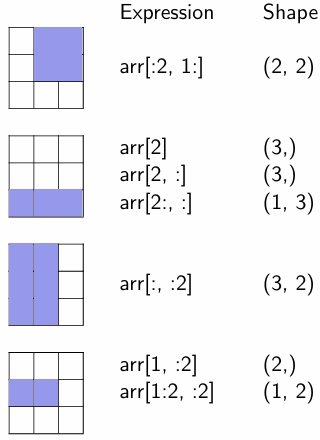
\includegraphics[width = 0.181\textwidth]{chapter 2/ch2_figure1.jpeg}
    \caption{Numpy Array Indexing}
\end{figure}
\newpage
\textcolor{teal}{\paragraph{Integer Array Indexing}}
\textcolor{cyan}{Integer array indexing} allows us to \hl{construct arbitrary arrays using the data from another array}.\\
\begin{egBox}{Example 2.2.4.4}{}
    \begin{lstlisting}[language=Python, basicstyle=\ttfamily\small, keywordstyle=\color{blue}, commentstyle=\color{forestgreen}, stringstyle=\color{red}, showstringspaces=false]
import numpy as np

a = np.array([[1, 2], [3, 4], [5, 6]])

# An example of integer array indexing.
# The returned array will have shape (3,)
print(a[[0, 1, 2], [0, 1, 0]])                  # Prints "[1 4 5]"

# The above example of integer array indexing is equivalent to this:
print(np.array([a[0, 0], a[1, 1], a[2, 0]]))    # Prints "[1 4 5]"

# When using integer array indexing, we can reuse the same element from the source array:
print(a[[0, 0], [1, 1]])                        # Prints "[2 2]"

# Equivalent to the previous integer array indexing example
print(np.array([a[0, 1], a[0, 1]]))             # Prints "[2 2]"
    \end{lstlisting}
\end{egBox}
One trick of integer array indexing is \hl{selecting or mutating one element from each row of a matrix}.
\begin{egBox}{Example 2.2.4.5}{}
    \begin{lstlisting}[language=Python, basicstyle=\ttfamily\small, keywordstyle=\color{blue}, commentstyle=\color{forestgreen}, stringstyle=\color{red}, showstringspaces=false]
import numpy as np

# Create a new array from which we will select elements
a = np.array([[1, 2, 3], [4, 5, 6], [7, 8, 9], [10, 11, 12]])
print(a)                                        # Prints "array([[ 1,  2,  3],
                                                #                [ 4,  5,  6],
                                                #                [ 7,  8,  9],
                                                #                [10, 11, 12]])"

# Create an array of indices
b = np.array([0, 2, 0, 1])

# Select one element from each row of a using the indices in b
print(a[np.arange(4), b])                       # Prints "[ 1  6  7 11]"

# Mutate one element from each row of a using the indices in b
a[np.arange(4), b] += 10
print(a)                                        # Prints "array([[11,  2,  3],
                                                #                [ 4,  5, 16],
                                                #                [17,  8,  9],
                                                #                [10, 21, 12]])"
    \end{lstlisting}
\end{egBox}
\newpage
\textcolor{teal}{\paragraph{Boolean Array Indexing}}
\textcolor{cyan}{Boolean array indexing} allows us to \textcolor{violet}{pick out arbitrary elements} of an array.\\
It is often used to \textcolor{violet}{select elements of an array that satisfy some condition}.
\begin{egBox}{Example 2.2.4.6}{}
    \begin{lstlisting}[language=Python, basicstyle=\ttfamily\small, keywordstyle=\color{blue}, commentstyle=\color{forestgreen}, stringstyle=\color{red}, showstringspaces=false]
import numpy as np

a = np.array([[1, 2], [3, 4], [5, 6]])

bool_idx = (a > 2)          # Find the elements of a that are bigger than 2;
                            # This returns a numpy array of Booleans of the same shape as a,
                            # where each slot of bool_idx tells whether a > 2.

print(bool_idx)             # Prints "[[False False]
                            #          [ True  True]
                            #          [ True  True]]"

# We use boolean array indexing to construct a rank 1 array
# consisting of the elements of a corresponding to the True values of bool_idx
print(a[bool_idx])          # Prints "[3 4 5 6]"

# We can do all of the above in a single concise statement:
print(a[a > 2])             # Prints "[3 4 5 6]"
    \end{lstlisting}
\end{egBox}
\textcolor{olive}{\subsubsection{Data Types}}
Every numpy array is a grid of elements of the \textcolor{violet}{same type}.\\
Numpy \textcolor{violet}{provides a large set of numeric data types} that we can use to construct arrays.\\
Numpy tries to guess a data type when we create an array, but \textcolor{violet}{functions that construct arrays} usually also include an \textcolor{violet}{optional argument to explicitly specify the data type}.
\begin{egBox}{Example 2.2.4.7}{}
    \begin{lstlisting}[language=Python, basicstyle=\ttfamily\small, keywordstyle=\color{blue}, commentstyle=\color{forestgreen}, stringstyle=\color{red}, showstringspaces=false]
            import numpy as np

            x = np.array([1, 2])                    # Let numpy choose the datatype
            print(x.dtype)                          # Prints "int64"

            x = np.array([1.0, 2.0])                # Let numpy choose the datatype
            print(x.dtype)                          # Prints "float64"

            x = np.array([1, 2], dtype=np.int64)    # Force a particular datatype
            print(x.dtype)                          # Prints "int64"
    \end{lstlisting}
\end{egBox}
\newpage
\textcolor{olive}{\subsubsection{Array Math}}
\textcolor{teal}{\paragraph{Elementwise Operations}}
\textcolor{cyan}{Basic mathematical functions}  \textcolor{violet}{operate elementwise on arrays}, and are available both as \textcolor{violet}{operator overloads} and as \textcolor{violet}{functions in the numpy module}.

\begin{egBox}{Example 2.2.4.8}{}
    \begin{lstlisting}[language=Python, basicstyle=\ttfamily\small, keywordstyle=\color{blue}, commentstyle=\color{forestgreen}, stringstyle=\color{red}, showstringspaces=false]
                    import numpy as np

                    x = np.array([[1, 2], [3, 4]], dtype=np.float64)
                    y = np.array([[5, 6], [7, 8]], dtype=np.float64)

                    # Elementwise sum; both produce the array
                    print(x + y)
                    print(np.add(x, y))         # [[ 6.0  8.0]
                                                #  [10.0 12.0]]

                    # Elementwise difference; both produce the array
                    print(x - y)
                    print(np.subtract(x, y))    # [[-4.0 -4.0]
                                                #  [-4.0 -4.0]]

                    # Elementwise product; both produce the array
                    print(x * y)
                    print(np.multiply(x, y))    # [[ 5.0 12.0]
                                                #  [21.0 32.0]]

                    # Elementwise division; both produce the array
                    print(x / y)
                    print(np.divide(x, y))      # [[0.2        0.33333333]
                                                #  [0.42857143 0.5       ]]

                    # Elementwise square root; produces the array
                    print(np.sqrt(x))           # [[1.         1.41421356]
                                                #  [1.73205081 2.        ]]
    \end{lstlisting}
\end{egBox}
\textcolor{teal}{\paragraph{Vector, Matrix and Tensor}}
\FloatBarrier
\begin{wrapfigure}[6]{r}{0.3\textwidth}
    \centering
    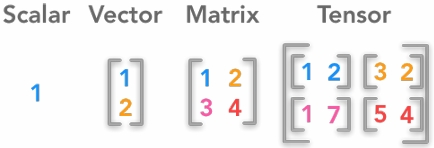
\includegraphics[width = 0.3\textwidth]{chapter 2/ch2_figure2.jpeg}
    \caption{Scalar, Vector, Matrix and Tensor}
\end{wrapfigure}
Here are the definitions of Scalars, Vectors, Matrices and Tensors:\\
\begin{description}    
    \item[$\bullet$] \textcolor{cyan}{Scalars}: Single numbers.
    \item[$\bullet$] \textcolor{cyan}{Vectors}: 1-Dimensional arrays of numbers.
    \item[$\bullet$] \textcolor{cyan}{Matrices}: 2-Dimensional arrays of numbers.
    \item[$\bullet$] \textcolor{cyan}{Tensors}: Multi-Dimensional arrays of numbers.
\end{description}
They are useful in \textcolor{violet}{expressing numerical information} and 
\textcolor{violet}{different mathematical operations}.
\textcolor{teal}{\paragraph{Dot Product}}
\textcolor{cyan}{Dot Product} is the \textcolor{violet}{sum of products of values} in \textcolor{cyan}{two same-sized vectors (arrays)}.\\
The output of the dot product is a \textcolor{violet}{scalar}.\\
\begin{figure}[h]
    \centering
    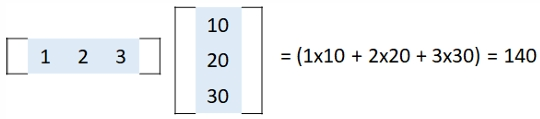
\includegraphics[scale=0.75]{chapter 2/ch2_figure3.jpeg}
    \caption{Dot Product}
\end{figure}
Dot product can be performed using the \textcolor{red}{\texttt{np.dot()}} function/method.\\
\textcolor{red}{\texttt{np.dot()}} is available both as a \textcolor{violet}{function in the numpy module} and as a \textcolor{violet}{method of array objects}.
\newpage
\begin{egBox}{Example 2.2.4.9}{}
    \begin{lstlisting}[language=Python, basicstyle=\ttfamily\small, keywordstyle=\color{blue}, commentstyle=\color{forestgreen}, stringstyle=\color{red}, showstringspaces=false]
            import numpy as np

            x = np.array([[1, 2], [3, 4]])
            y = np.array([[5, 6], [7, 8]])
            v = np.array([9, 10])
            w = np.array([11, 12])

            # Dot product of two vectors; both produce 219
            print(v.dot(w))
            print(np.dot(v, w))

            # Matrix / vector product; both produce the rank 1 array [29 67]
            print(x.dot(v))
            print(np.dot(x, v))

            # Matrix / matrix product; both produce the rank 2 array    [[19 22]
            #                                                            [43 50]]
            print(x.dot(y))
            print(np.dot(x, y))     
    \end{lstlisting}
\end{egBox}
\textcolor{teal}{\paragraph{Matrix Multiplication}}
\textcolor{cyan}{Matrix Multiplication} is one of the most important operations for artificial intelligence.\\
It is a \textcolor{violet}{matrix version of the dot product with two matrices}.\\
The output of the matrix multiplication is a \textcolor{violet}{matrix} whose \textcolor{violet}{rows are the first matrix} and \textcolor{violet}{columns are the second matrix}.\\
\begin{figure}[h]
    \centering
    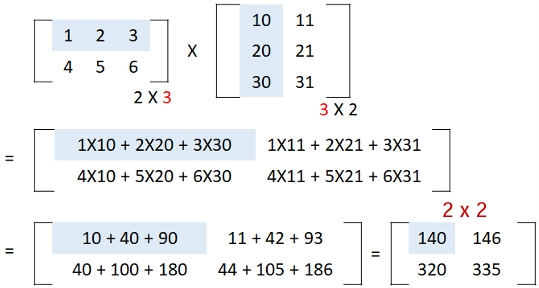
\includegraphics[scale=0.8]{chapter 2/ch2_figure4.jpeg}
    \caption{Matrix Multiplication}
\end{figure}
Matrix multiplication can be performed using the \textcolor{red}{\texttt{np.matmul()}} function/method or \textcolor{red}{\texttt{@}} operator.\\
\begin{description}
    \item[$\bullet$] Matrix multiplication can be performed by dot method, matmul method or @ operator (Python 3.5 or above).
    \item[$\bullet$] However, when we deal with N-dimensional arrays with \(N>2\), the result produced by dot and matmul may be different.
    \item[$\therefore$] It is recommended to use matmul method or @ operator for matrix multiplication.
\end{description}
\newpage
\textcolor{red}{\texttt{np.matmul()}} or \textcolor{red}{\texttt{@}} is \textcolor{violet}{only available as a function in the numpy module}.
\begin{egBox}{Example 2.2.4.10}{}
    \begin{lstlisting}[language=Python, basicstyle=\ttfamily\small, keywordstyle=\color{blue}, commentstyle=\color{forestgreen}, stringstyle=\color{red}, showstringspaces=false]
            import numpy as np

            x = np.array([[1, 2], [3, 4]])
            y = np.array([[5, 6], [7, 8]])
            v = np.array([9, 10])
            w = np.array([11, 12])

            # Inner product of vectors; both produce 219
            print(np.matmul(v, w))
            print(v @ w)

            # Matrix / vector product; both produce the rank 1 array [29 67]
            print(np.matmul(x, v))
            print(x @ v)

            # Matrix / matrix product; both produce the rank 2 array    [[19 22]
            #                                                             [43 50]]
            print(np.matmul(x, y))
            print(x @ y)            
    \end{lstlisting}
\end{egBox}
\textcolor{teal}{\paragraph{Numpy Functions}}
Numpy provides \textcolor{violet}{many useful functions for performing computations on arrays}, one of the most useful functions is \textcolor{red}{\texttt{np.sum()}}.
\begin{egBox}{Example 2.2.4.11}{}
    \begin{lstlisting}[language=Python, basicstyle=\ttfamily\small, keywordstyle=\color{blue}, commentstyle=\color{forestgreen}, stringstyle=\color{red}, showstringspaces=false]
            import numpy as np

            x = np.array([[1, 2], [3, 4]])

            print(np.sum(x))            # Compute sum of all elements; prints "10"
            print(np.sum(x, axis=0))    # Compute sum of each column; prints "[4 6]"
            print(np.sum(x, axis=1))    # Compute sum of each row; prints "[3 7]"
    \end{lstlisting}
\end{egBox}
\textcolor{olive}{\subsubsection{Transpose}}
The simplesr example of reshaping or otheriwse manipulate in arrays is the \textcolor{cyan}{transpose of a matrix}.
To transpose a matrix, simply use the \textcolor{blue}{T attribute of an array object} (\textcolor{red}{\texttt{x.T}}), \textcolor{blue}{transpose function} (\textcolor{red}{\texttt{np.transpose}(x)}) or \textcolor{blue}{transpose method of an array object} (\textcolor{red}{\texttt{x.transpose()}}).
\begin{egBox}{Example 2.2.4.12}{}
    \begin{lstlisting}[language=Python, basicstyle=\ttfamily\small, keywordstyle=\color{blue}, commentstyle=\color{forestgreen}, stringstyle=\color{red}, showstringspaces=false]
                            import numpy as np

                            x = np.array([[1, 2], [3, 4]])
                            print(x)                # Prints "[[1 2]
                                                    #          [3 4]]"
                            print(x.T)              # Prints "[[1 3]
                                                    #          [2 4]]"
                            print(np.transpose(x))  # Prints "[[1 3]
                                                    #          [2 4]]"
                            print(x.transpose())    # Prints "[[1 3]
                                                    #          [2 4]]"
    \end{lstlisting}
\end{egBox}
They are used to \textcolor{violet}{reverse the dimensions of the given array} (It changes the row to column and column to row).
\newpage
The transpose function comes with \textcolor{violet}{axes parameter} which, according to the values specified to the axes parameter, \textcolor{violet}{permutes the array}.
\begin{wrapfigure}[1]{r}{0.3\textwidth}
    \centering
    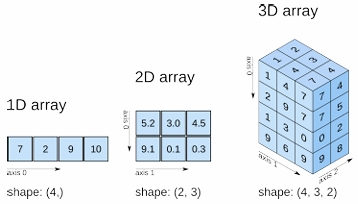
\includegraphics[width = 0.3\textwidth]{chapter 2/ch2_figure5.jpeg}
    \caption{Transpose}
\end{wrapfigure}
\begin{synBox}{Syntax 2.9}{Transpose}
    \begin{lstlisting}[language=Python, basicstyle=\ttfamily\small, keywordstyle=\color{blue}, commentstyle=\color{forestgreen}, stringstyle=\color{red}, showstringspaces=false]
                    np.transpose(arr, axis)
    \end{lstlisting}
    \raggedright
    where:\\
    \begin{description}
        \item[$\bullet$] \textcolor{brown}{\texttt{arr}}: Array we want to transpose.
        \item[$\bullet$] \textcolor{brown}{\texttt{axis}}: By default, the value is \texttt{None}. When \texttt{None} or no value is passed, it will reverse the dimensions of array arr.\\
        If specified. it must be the tuple or list, which contains the parameters of [0,1, ..., N-1] where N is the number of axes of arr.
    \end{description}
\end{synBox}

\begin{egBox}{Example 2.2.4.13}{}
    \begin{lstlisting}[language=Python, basicstyle=\ttfamily\small, keywordstyle=\color{blue}, commentstyle=\color{forestgreen}, stringstyle=\color{red}, showstringspaces=false]
import numpy as np

# Create a 3D array (2 layers, 3 rows, 4 columns) with numbers 0 to 23
arr = np.array([[[0, 1, 2, 3],
                 [4, 5, 6, 7],
                 [8, 9, 10, 11]],
                [[12, 13, 14, 15],
                 [16, 17, 18, 19],
                 [20, 21, 22, 23]]])

    \end{lstlisting}
\textcolor{orange}{Transpose can re-order the array axes.}\\
\textcolor{orange}{For example, if we want to take the current last axis (axis 2), make it the axis 0 (put 2 at the front), take the current first axis (axis 0), make it the axis 1 (put 0 in the middle), take the current second axis (axis 1) and make it the axis 2 (put 1 at the end).}
    \begin{lstlisting}[language=Python, basicstyle=\ttfamily\small, keywordstyle=\color{blue}, commentstyle=\color{forestgreen}, stringstyle=\color{red}, showstringspaces=false]
# Transpose the array arr with axes [2, 0, 1]
print(np.transpose(arr, [2, 0, 1]))
# Same output as np.transpose(arr, [2, 0, 1])
print(arr.transpose([2, 0, 1]))

# Output:

# [[[ 0  4  8]
#   [12 16 20]]

#  [[ 1  5  9]
#   [13 17 21]]

#  [[ 2  6 10]
#   [14 18 22]]

#  [[ 3  7 11]
#   [15 19 23]]]
    \end{lstlisting}
\end{egBox}
However, taking the transpose of a \textcolor{violet}{rank 1 array} will \textcolor{violet}{not change the array}.
\begin{egBox}{Example 2.2.4.14}{}
    \begin{lstlisting}[language=Python, basicstyle=\ttfamily\small, keywordstyle=\color{blue}, commentstyle=\color{forestgreen}, stringstyle=\color{red}, showstringspaces=false]
                            import numpy as np

                            x = np.array([1, 2, 3])
                            print(x)                # Prints "[1 2 3]"
                            print(x.T)              # Prints "[1 2 3]"
                            print(np.transpose(x))  # Prints "[1 2 3]"
                            print(x.transpose())    # Prints "[1 2 3]"
    \end{lstlisting}
\end{egBox}
\newpage
\textcolor{olive}{\subsubsection{Reshaping}}
\textcolor{cyan}{Reshaping} means \textcolor{violet}{changing the shape of an array} (number of elements in each dimension).\\
By reshaping, we can \textcolor{violet}{add or remove dimensions} or \textcolor{violet}{change the number of elements in each dimension}.\\
It can be done using the \textcolor{red}{\texttt{np.reshape()}} function/method.
\begin{synBox}{Syntax 2.10}{Reshape}
    \begin{lstlisting}[language=Python, basicstyle=\ttfamily\small, keywordstyle=\color{blue}, commentstyle=\color{forestgreen}, stringstyle=\color{red}, showstringspaces=false]
                                    np.reshape(arr, newshape)
    \end{lstlisting}
    \raggedright
    where:\\
    \begin{description}
        \item[$\bullet$] \textcolor{brown}{\texttt{arr}}: Array to be reshaped.
        \item[$\bullet$] \textcolor{brown}{\texttt{newshape}}: int or tuple of ints.\\
        The new shape should be compatible with the original shape.\\
        If it is an integer, then the result will be a 1-D array of that length.\\
        If the one shape dimension can be -1, the value is inferred from the length of the array and remaining dimensions.
    \end{description}
\end{synBox}
\begin{egBox}{Example 2.2.4.15}{}
    \begin{lstlisting}[language=Python, basicstyle=\ttfamily\small, keywordstyle=\color{blue}, commentstyle=\color{forestgreen}, stringstyle=\color{red}, showstringspaces=false]
                import numpy as np

                arr1 = np.array([1, 2, 3, 4, 5, 6, 7, 8, 9, 10, 11, 12])
                arr2 = arr1.reshape(4, 3)   # Convert arr1 into a 4x3 matrix
                arr2 = arr1.reshape(4, -1)  # Same output as arr1.reshape(4, 3)

                print(arr2) # Output: [[ 1  2  3]
                            #          [ 4  5  6]
                            #          [ 7  8  9]
                            #          [10 11 12]]

                print(arr2.shape) # Output: (4, 3)

                # Create a 3D array (2 layers, 3 rows, 4 columns) with numbers 0 to 23
                arr3 = np.arangge(24).reshape(2, 3, 4)

                print(arr3) # Output: [[[ 0  1  2  3]
                            #          [ 4  5  6  7]
                            #          [ 8  9 10 11]]
                            #         [[12 13 14 15]
                            #          [16 17 18 19]
                            #          [20 21 22 23]]]
    \end{lstlisting}
\end{egBox}
\textcolor{olive}{\subsubsection{Increasing the Dimensions of an Array}}
\textcolor{teal}{\paragraph{New Axis}}
\textcolor{cyan}{New Axis} is used to \textcolor{violet}{increase the dimensions of an array} by \textcolor{violet}{adding a new axis} at a specific position.\\
It can be done using the \textcolor{red}{\texttt{np.newaxis}} attribute, which is \textcolor{violet}{an alias} for \textcolor{blue}{\texttt{None}}.
\begin{synBox}{Syntax 2.11}{New Axis}
    \begin{lstlisting}[language=Python, basicstyle=\ttfamily\small, keywordstyle=\color{blue}, commentstyle=\color{forestgreen}, stringstyle=\color{red}, showstringspaces=false]
                                            np.newaxis
    \end{lstlisting}
    \raggedright
    \begin{description}
        \item[$\bullet$] Usage: Placing \textcolor{red}{\texttt{numpy.newaxis}} inside [ ] adds a new dimension of size 1 at that position.
    \end{description}
\end{synBox}
\newpage
\begin{egBox}{Example 2.2.4.16}{}
    \begin{lstlisting}[language=Python, basicstyle=\ttfamily\small, keywordstyle=\color{blue}, commentstyle=\color{forestgreen}, stringstyle=\color{red}, showstringspaces=false]
                    import numpy as np
                    
                    arr1 = np.array([1, 2, 3, 4, 5])        # [1 2 3 4 5]
                    
                    # Convert 1D array to a column matrix.
                    arr2 = arr1[np.newaxis, :]              # [[1 2 3 4 5]]

                    # Convert 1D array to a column matrix.
                    arr3 = arr1[None]                       # [[1 2 3 4 5]]

                    arr4 = np.array([1, 2, 3], [4, 5, 6])   # [[1 2 3]
                                                            #  [4 5 6]]

                    arr5 = arr4[np.newaxis]                 # [[[1 2 3]
                                                            #   [4 5 6]]]
    \end{lstlisting}
\end{egBox}
\begin{egBox}{Example 2.2.4.17}{}
    \begin{lstlisting}[language=Python, basicstyle=\ttfamily\small, keywordstyle=\color{blue}, commentstyle=\color{forestgreen}, stringstyle=\color{red}, showstringspaces=false]
    import numpy as np

    arr1 = np.array([[1, 2, 3], [4, 5, 6]])
    print(arr1)                 # [[1 2 3]
                                #  [4 5 6]]

    # np.newaxis means adding a new dimension of size 1 (1 column)
    arr2 = arr1[:, :, np.newaxis]  # Equivalent to arr2 = arr1[..., np.newaxis]

    print(arr2)                 # [[[1]
                                #   [2]
                                #   [3]]
                                #  [[4]
                                #   [5]
                                #   [6]]]

    print(arr2.shape)           # (2, 3, 1), meaning 2 layers, 3 rows, 1 column
    \end{lstlisting}
\end{egBox}
\begin{egBox}{Example 2.2.4.18}{}
    \begin{lstlisting}[language=Python, basicstyle=\ttfamily\small, keywordstyle=\color{blue}, commentstyle=\color{forestgreen}, stringstyle=\color{red}, showstringspaces=false]
    import numpy as np

    arr1 = np.array([[1, 2, 3], [4, 5, 6]])
    print(arr1)                 # [[1 2 3]
                                #  [4 5 6]]

    # np.newaxis means adding a new dimension of size 1 (1 row) and highest dimension (column)
    arr2 = arr1[:, np.newaxis, :]

    print(arr2)                 # [[[1 2 3]
                                #   [4 5 6]]]

    print(arr2.shape)           # (2, 1, 3), meaning 2 layers, 1 row, 3 columns
    \end{lstlisting}
\end{egBox}
\newpage
\textcolor{teal}{\paragraph{Expand Dimensions}}
\textcolor{cyan}{Expand Dimensions} is used to \textcolor{violet}{increase the dimensions of an array} by \textcolor{violet}{adding a new axis} at a specific position.\\
It can be done using the \textcolor{red}{\texttt{np.expand\_dims()}} function/method.
\begin{synBox}{Syntax 2.12}{Expand Dimensions}
    \begin{lstlisting}[language=Python, basicstyle=\ttfamily\small, keywordstyle=\color{blue}, commentstyle=\color{forestgreen}, stringstyle=\color{red}, showstringspaces=false]
                                        np.expand_dims(arr, axis)
    \end{lstlisting}
    \raggedright
    where:\\
    \begin{description}
        \item[$\bullet$] \textcolor{brown}{\texttt{arr}}: Input array.
        \item[$\bullet$] \textcolor{brown}{\texttt{axis}}: int or tuple of ints, in which the position in the expanded axes where the new axis is placed.
    \end{description}
\end{synBox}
\begin{egBox}{Example 2.2.4.19}{}
    \begin{lstlisting}[language=Python, basicstyle=\ttfamily\small, keywordstyle=\color{blue}, commentstyle=\color{forestgreen}, stringstyle=\color{red}, showstringspaces=false]
import numpy as np

arr1 = np.array([1, 2, 3], [4, 5, 6])
print(arr1)                 # [[1 2 3]
                            #  [4 5 6]]

arr2 = np.expand_dims(arr1, 2) # 2 means adding a new dimensioon of size 1 after 2nd dimension
print(arr2)                 # [[[1]
                            #   [2]
                            #   [3]]
                            #  [[4]
                            #   [5]
                            #   [6]]]

print(arr2.shape)           # (2, 3, 1), meaning 2 layers, 3 rows, 1 column
    \end{lstlisting}
\end{egBox}
\begin{egBox}{Example 2.2.4.20}{}
    \begin{lstlisting}[language=Python, basicstyle=\ttfamily\small, keywordstyle=\color{blue}, commentstyle=\color{forestgreen}, stringstyle=\color{red}, showstringspaces=false]
import numpy as np

arr1 = np.array([1, 2, 3], [4, 5, 6])
print(arr1)                 # [[1 2 3]
                            #  [4 5 6]]

arr2 = np.expand_dims(arr1, 1) # 1 means adding a new dimensioon of size 1 after 1st dimension
print(arr2)                 # [[[1 2 3]]
                            #  [[4 5 6]]]

print(arr2.shape)           # (2, 1, 3), meaning 2 layers, 1 row, 3 columns
    \end{lstlisting}
\end{egBox}
\textcolor{olive}{\subsubsection{Broadcasting}}

\textcolor{cyan}{Broadcasting} is a powerful mechanism that \textcolor{violet}{allows numpy to work with arrays of different shapes} when performing arithmetic operations.\\

Frequently we have a smaller array and a larger array, and we want to use the smaller array multiple times to perform some operation on the larger array.\\

Broadcasting solves the problems of \textcolor{violet}{arithmetic operations between arrays of different shapes} by \textcolor{violet}{replicating the smaller array along the last mismatched dimension}.\\

\begin{figure}[h]
    \centering
    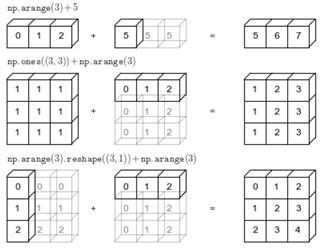
\includegraphics[scale=0.36]{chapter 2/ch2_figure6.jpeg}
    \caption{Broadcasting}
\end{figure}
\newpage
\textcolor{teal}{\paragraph{Difference between Explicit loop and Broadcasting}}
\textcolor{cyan}{Numpy broadcasting} allows us to perform this \textcolor{violet}{computation without actually creating multiple copies of the smaller array}.\\
However, if we use the \textcolor{cyan}{explicit loop}, we will have to \textcolor{violet}{create multiple copies of the smaller array} to perform the operation, which is \textcolor{violet}{inefficient}.
\begin{egBox}{Example 2.2.4.21}{}
    \begin{description}
        \item[$\bullet$] \textcolor{blue}{Explicit Loop}: Computation time is \textcolor{violet}{slow} when the matrix is very large.
        \begin{lstlisting}[language=Python, basicstyle=\ttfamily\small, keywordstyle=\color{blue}, commentstyle=\color{forestgreen}, stringstyle=\color{red}, showstringspaces=false]
import numpy as np

# Add the vector v to each row of the matrix x, storing the result in the matrix y
x = np.array([[1, 2, 3], [4, 5, 6], [7, 8, 9], [10, 11, 12]])
v = np.array([1, 0, 1])
y = np.empty_like(x)        # Create an empty matrix with the same shape as x

# Add the vector v to each row of the matrix x with an explicit loop
for i in range(4):
    y[i, :] = x[i, :] + v

print(y)                    # Prints "[[ 2  2  4]
                            #          [ 5  5  7]
                            #          [ 8  8 10]
                            #          [11 11 13]]"
            
        \end{lstlisting}
        \item[$\bullet$] \textcolor{blue}{Broadcasting}: Computation time is \textcolor{violet}{fast} when the matrix is very large.\\
        Adding the vector v to each row of the matrix x is equivalent to forming a matrix vv by stacking multiple copies of v vertically, then performing elementwise summation of x and vv.
        \begin{lstlisting}[language=Python, basicstyle=\ttfamily\small, keywordstyle=\color{blue}, commentstyle=\color{forestgreen}, stringstyle=\color{red}, showstringspaces=false]
import numpy as np

# Add the vector v to each row of the matrix x, storing the result in the matrix y
x = np.array([[1, 2, 3], [4, 5, 6], [7, 8, 9], [10, 11, 12]])
v = np.array([1, 0, 1])

vv = np.tile(v, (4, 1))     # Stack 4 copies of v on top of each other

print(vv)                   # Prints "[[1 0 1]
                            #          [1 0 1]
                            #          [1 0 1]
                            #          [1 0 1]]"

y = x + vv                  # Add x and vv elementwise

print(y)                    # Prints "[[ 2  2  4]
                            #          [ 5  5  7]
                            #          [ 8  8 10]
                            #          [11 11 13]]"
        \end{lstlisting}
    \end{description}
\end{egBox}
\begin{egBox}{Example 2.2.4.22}{}
    \begin{lstlisting}[language=Python, basicstyle=\ttfamily\small, keywordstyle=\color{blue}, commentstyle=\color{forestgreen}, stringstyle=\color{red}, showstringspaces=false]
import numpy as np

# Add the vector v to each row of the matrix x, storing the result in the matrix y
x = np.array([[1, 2, 3], [4, 5, 6], [7, 8, 9], [10, 11, 12]])
v = np.array([1, 0, 1])

y = x + v  # Add v to each row of x using broadcasting

print(y)  # Prints "[[ 2  2  4]
          #          [ 5  5  7]
          #          [ 8  8 10]
          #          [11 11 13]]"

    \end{lstlisting}
    $\therefore$ The line y = x + v works even though x has shape (4, 3) and v has shape (3,) due to broadcasting; this line works as if v actually had shape (4, 3), where each row was a copy of v, and the sum was performed elementwise.
\end{egBox}
\newpage
\textcolor{teal}{\paragraph{Broadcasting Rules}}
Broadcasting follows a set of rules to determine the interaction between two arrays:
\begin{description}
    \item[$\bullet$] \textcolor{blue}{Rule 1}: \\
    If the two arrays do not have the same rank, prepend the shape of the lower rank array with 1s until both shapes have the same length.
    \item[$\bullet$] \textcolor{blue}{Rule 2}: \\
    The two arrays are compatible in a dimension if they have the same size in the dimension, or if one of the arrays has size 1 in that dimension.
    \item[$\bullet$] \textcolor{blue}{Rule 3}: \\
    The arrays can be broadcast together if they are compatible in all dimensions.
    \item[$\bullet$] \textcolor{blue}{Rule 4}: \\
    After broadcasting, each array behaves as if it had shape equal to the elementwise maximum of shapes of the two input arrays.
    \item[$\bullet$] \textcolor{blue}{Rule 5}: \\
    In any dimension where one array had size 1 and the other array had size greater than 1, the first array behaves as if it were copied along that dimension.
\end{description}
\begin{egBox}{Example 2.2.4.23}{}
    \raggedright
    \textbf{Question:} Given two arrays \texttt{A = np.array([1, 2, 3])} and \texttt{B = np.array([2])}. Can we perform \texttt{A * B}? \\
    
    \textbf{Answer:} \\
    
    \begin{lstlisting}[language=Python, basicstyle=\ttfamily\small, keywordstyle=\color{blue}, commentstyle=\color{forestgreen}, stringstyle=\color{red}, showstringspaces=false]
                                    import numpy as np

                                    A = np.array([1, 2, 3])
                                    print(A.ndim)   # 1
                                    print(A.shape)  # (3,)

                                    B = np.array([2])
                                    print(B.ndim)   # 1
                                    print(B.shape)  # (1,)

                                    print(A*B)      # [2 4 6]
    \end{lstlisting}
    $\because$ Rank of A is 1 and Rank of B is 1. They have the same rank.\\
    $\therefore$ They are compatilbe in all dimensions since array B has size 1 in that dimension, and hence we can perform A*B.
\end{egBox}
\begin{egBox}{Example 2.2.4.24}{}
    \raggedright
    \textbf{Question:} Given two arrays \texttt{A = np.array([1, 2, 3])} and \texttt{B = np.array([[4, 4, 4], [3, 3, 3]])}. Can we perform \texttt{A * B}? \\
    \textbf{Answer:} \\
    \begin{lstlisting}[language=Python, basicstyle=\ttfamily\small, keywordstyle=\color{blue}, commentstyle=\color{forestgreen}, stringstyle=\color{red}, showstringspaces=false]
                                    import numpy as np

                                    A = np.array([1, 2, 3])
                                    print(A.ndim)   # 1
                                    print(A.shape)  # (3,)

                                    B = np.array([[4, 4, 4], [3, 3, 3]])
                                    print(B.ndim)   # 2
                                    print(B.shape)  # (2, 3)

                                    print(A*B)      # [[ 4  8 12]
                                                    #  [ 3  6  9]]
    \end{lstlisting}
    $\because$ Rank of A is 1 and Rank of B is 2. They do not have the same rank. But we can prepend the shape of the lower rank array (array A) with 1s until both shapes have the same length.\\
    $\therefore$ They are compatilbe in all dimensions since array A has size 1 in that dimension, and hence we can perform A*B.
\end{egBox}
\newpage
\begin{egBox}{Example 2.2.4.25}
    \raggedright
    \raggedright
    \textbf{Questions:} For each of the following pairs, state whether they are compatible for broadcasting. If they are, what is the size of the resulting array after performing \texttt{A * B}?\\

    \begin{enumerate}
        \item Pair 1: A: Shape 5 x 4, B: Shape 1 \\
            \underline{\textbf{Answer:}} \textcolor{red}{Compatible. Resulting array shape: 5 x 4}
        \item Pair 2: A: Shape 5 x 4, B: Shape 4 \\
            \underline{\textbf{Answer:}} \textcolor{red}{Compatible. Resulting array shape: 5 x 4}
        \item Pair 3: A: Shape 15 x 3 x 5, B: Shape 15 x 1 x 5 \\
            \underline{\textbf{Answer:}} \textcolor{red}{Compatible. Resulting array shape: 15 x 3 x 5}
        \item Pair 4: A: Shape 15 x 3 x 5, B: Shape 3 x 5 \\
            \underline{\textbf{Answer:}} \textcolor{red}{Compatible. Resulting array shape: 15 x 3 x 5}
        \item Pair 5: A: Shape 15 x 3 x 5, B: Shape 3 x 1 \\
            \underline{\textbf{Answer:}} \textcolor{red}{Compatible. Resulting array shape: 15 x 3 x 5}
        \item Pair 6: A: Shape 16 x 6 x 7, B: Shape 16 x 6 \\
            \underline{\textbf{Answer:}} \textcolor{red}{Not Compatible}
    \end{enumerate}
\end{egBox}
\textcolor{teal}{\paragraph{Broadcasting in Practice}}
\textcolor{cyan}{Broadcasting operations} are \textcolor{violet}{useful in simplifying the calculation of mathematical operations} on arrays. \\
There are two examples of showing its usefulness of broadcasting operations:\\
\vspace{2mm}
\textcolor{darkgray}{\underline{\textbf{Example 1: Centering an Array}}}\\
\vspace{1mm}
Suppose we have a grade book for 5 students, each of whom have taken 3 exams. We store the grades in a 5 x 3 array.\\
\begin{lstlisting}[language=Python, basicstyle=\ttfamily\small, keywordstyle=\color{blue}, commentstyle=\color{forestgreen}, stringstyle=\color{red}, showstringspaces=false]
            import numpy as np
            scores = np.array([[1, 2, 3], [4, 5, 6], [7, 8, 9], [10, 11, 12], [13, 14, 15]])
\end{lstlisting}
We can compute the mean of each exam using the \textcolor{red}{\texttt{np.mean()}} function/method across the first dimension.
\begin{lstlisting}[language=Python, basicstyle=\ttfamily\small, keywordstyle=\color{blue}, commentstyle=\color{forestgreen}, stringstyle=\color{red}, showstringspaces=false]
                    score_mean = scores.mean(0) # 0 means the first dimension
                    print(score_mean)           # [7. 8. 9.]
\end{lstlisting}
To center the scores arrays, we can subtract the mean from the scores (broadcasting operation).
\begin{lstlisting}[language=Python, basicstyle=\ttfamily\small, keywordstyle=\color{blue}, commentstyle=\color{forestgreen}, stringstyle=\color{red}, showstringspaces=false]
                        centered_scores = scores - score_mean
                        print(centered_scores)      # [[-6. -6. -6.]
                                                    #  [-3. -3. -3.]
                                                    #  [ 0.  0.  0.]
                                                    #  [ 3.  3.  3.]
                                                    #  [ 6.  6.  6.]]
\end{lstlisting}
We check the centered array has zero mean.
\begin{lstlisting}[language=Python, basicstyle=\ttfamily\small, keywordstyle=\color{blue}, commentstyle=\color{forestgreen}, stringstyle=\color{red}, showstringspaces=false]
                        print(centered_scores.mean(0))  # [0. 0. 0.]
\end{lstlisting}
\vspace{2mm}
\textcolor{darkgray}{\underline{\textbf{Example 2: Pairwise Distances}}}\\
\vspace{1mm}
Suppose we have two 2D arrays, \texttt{X} of shape (M, D) and \texttt{Y} of shape (N, D). They have different numbers of rows but the same number of columns.\\
We wish to compute the Euclidean distance between each row of \texttt{X} and each row of \texttt{Y}.\\
If a given row of x is represented by D numbers (\(x_0, x_1, ..., x_{D-1}\)) and a given row of y is represented by D numbers (\(y_0, y_1, ..., y_{D-1}\)), the Euclidean distance between the two rows is: \\
\[
    \sqrt{(x_0 - y_0)^2 + (x_1 - y_1)^2 + ... + (x_{D-1} - y_{D-1})^2}
\]
We can do this using the following code:
\begin{figure}[h]
    \centering
    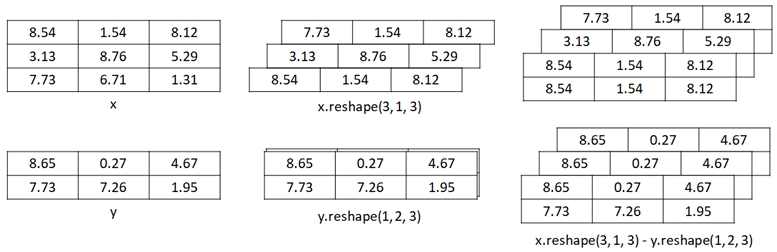
\includegraphics[scale=0.47]{chapter 2/ch2_figure7.jpeg}
    \caption{Pairwise Distances Code Illustration}
\end{figure}
\newpage
\begin{lstlisting}[language=Python, basicstyle=\ttfamily\small, keywordstyle=\color{blue}, commentstyle=\color{forestgreen}, stringstyle=\color{red}, showstringspaces=false]
        import numpy as np

        # Shape-(3, 3) array
        x = np.array([[8.54, 1.54, 8.12],
                      [3.13, 8.76, 5.29],
                      [7.73, 6.71, 1.31]])

        # Shape-(2, 3) array
        y = np.array([[8.65, 0.27, 4.67],
                      [7.73, 7.26, 1.95]])

        # We need to compute 6 Euclidean distances, one for each pair of rows from x and y
        # If x has shape (M, 3) and y has shape (N, 3), then the result should have shape (M, N)
        reshaped_x = x.reshape(3, 1, 3)
        reshaped_y = y.reshape(1, 2, 3)

        # Via broadcasting, diffs[i, j] = x[i] - y[j]
        diffs = reshaped_x - reshaped_y

        print(diffs.shape)                          # (3, 2, 3)

        print(diffs)                                # [[[-0.11  1.27  3.45]
                                                    #   [ 0.81 -5.72  6.17]]
                                                    #  [[-5.52  8.49  3.34]
                                                    #   [-4.6  -1.5   3.34]]
                                                    #  [[-0.92  6.44 -3.36]
                                                    #   [ 0.   -0.55 -0.64]]]

        # Compute the squared differences
        dists np.sqrt(np.sum(diffs ** 2, axis=2))   # axis=2 means the column axis

        print(dists)                                # [[ 3.67797499  8.45241977]
                                                    #  [10.14568381  5.87925165]
                                                    #  [ 7.32185769  0.84386018]]

        print(dists.shape)                          # (3, 2)
\end{lstlisting}
\subsection{Comparison between Numpy Arrays and Python Lists}
Numpy array contains a single pointer to one contiguous block of data.\\
Python list contains a pointer to a block of pointers, each of which points to a full Python object like the Python object for integers.\\
\begin{figure}[h]
    \centering
    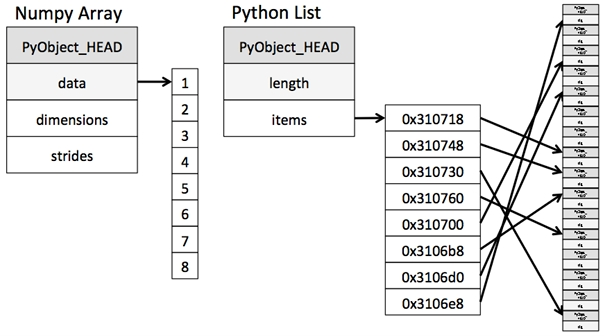
\includegraphics[scale=0.5]{chapter 2/ch2_figure8.jpeg}
    \caption{Comparison between Numpy Arrays and Python Lists}
\end{figure}
\newpage
Numpy arrays are better than Python lists in the following aspects:
\begin{enumerate}
    \item \hl{Less Memory}: Numpy arrays consume less memory than Python lists.
    \begin{egBox}{Example 2.2.5.1}{}
        \begin{lstlisting}[language=Python, basicstyle=\ttfamily\small, keywordstyle=\color{blue}, commentstyle=\color{forestgreen}, stringstyle=\color{red}, showstringspaces=false]
import numpy as np; import sys; import gc   # Import numpy package, sys and gc module

def actualsize(input_object):
    # memory_size: Actual memory size of "input_object" and initialize it to 0
    memory_size = 0 

    # ids: Empty set to store all the ids of the objects in "input_object"
    ids = set()

    # objects: List with "input_object" (Traverse from "input_object" to the end)
    objects = [input_object]

    while objects:                  # While "objects" is not empty
        new = []                    # new: Empty list to keep the items linked by "objects"
        for obj in objects:         # obj: Each object in "objects"
            if id(obj) not in ids:  # If the id of "obj" is not in "ids"
                ids.add(id(obj))    # Add the id of the "obj" to "ids"
                # Use sys.getsizeof() to get memory size of "obj" and add it to "memory_size"
                memory_size += sys.getsizeof(obj) 
                new.append(obj)     # Append "obj" to "new"
        
        # Update "objects" with the list of objecys directly referred to by *new        
        objects = gc.get_referents(*new)
    return memory_size              # Return "memory_size"

L = list(range(0, 1000))            # Create a Python list of 1000 elements
A = np.arange(1000)                 # Create a Numpy array of 1000 elements

# Print size of the whole Python list
print(actualsize(L))                # Output: 37116

# Print size of the whole Numpy array
print(actualsize(A))                # Output: 8104
        \end{lstlisting}
    \end{egBox}
    \item \hl{Fast}: Numpy arrays are faster than Python lists.
    \begin{egBox}{Example 2.2.5.2}{}
        \begin{lstlisting}[language=Python, basicstyle=\ttfamily\small, keywordstyle=\color{blue}, commentstyle=\color{forestgreen}, stringstyle=\color{red}, showstringspaces=false]
import numpy as np  # Import required packages
import time as T

size = 1000000  # Size of the arrays and lists

list1 = range(size) # Declare lists
list2 = range(size)
array1 = np.arange(size) # Declare Numpy arrays
array2 = np.arange(size)

# Capture time before the multiplication of Python lists
initial_time = T.time()
# Multiply elements of both the lists and stored in another list
result_list = [(a * b) for a, b in zip(list1, list2)]
# Calculate execution time, it prints "Time taken by Lists: 0.13024258613586426 s"
print("Time taken by Lists:", T.time() - initial_time, "s")

# Capture time before the multiplication of Numpy arrays
initial_time = T.time()
# Multiply elements of both the Numpy arrays and stored in another Numpy array
result_array = array1 * array2
# Calculate execution time, it prints "Time taken by Numpy Arrays: 0.006006956100463867 s"
print("Time taken by Numpy Arrays:", T.time() - initial_time, "s")
    \end{lstlisting}
\end{egBox}
\newpage
\item \hl{Convenient}: Numpy arrays are more convenient to use than Python lists.
    \begin{egBox}{Example 2.2.5.3}{}
        \begin{lstlisting}[language=Python, basicstyle=\ttfamily\small, keywordstyle=\color{blue}, commentstyle=\color{forestgreen}, stringstyle=\color{red},
        showstringspaces=false]
                import numpy as np      # Import Numpy package

                ls = [1, 2, 3]          # Python list
                arr = np.array(ls)      # Numpy array

                try:
                    ls += 4             # Try to add 4 to the Python list
                except(TypeError):
                    print("Lists do not support list + int operation")

                try:
                    arr += 4            # Try to add 4 to the Numpy array
                    print("Modified Numpy array:", arr)
                except(TypeError):
                    print("Numpy arrays do not support list + int operation")

                # Output:

                # Lists do not support list + int operation
                # Modified Numpy array: [5 6 7]
        \end{lstlisting}
    \end{egBox}
\end{enumerate}
\subsection{One-Hot Encoding}
\begin{defBox}{Definition 2.2.6}{One-Hot Encoding}
    \raggedright
    \textcolor{cyan}{One-Hot Encoding} is a process of \textcolor{red}{converting class vector (integers from 0 to number of classes) into a binary class matrix}.\\
\end{defBox}
In \textcolor{violet}{One-Hot Encoding}, each category is represented as a binary vector.\\
The vector has a length equal to the number of categories, and a 1 is placed in the position corresponding to the category.\\
\begin{synBox}{Syntax 2.13}{One-Hot Encoding}
    \begin{lstlisting}[language=Python, basicstyle=\ttfamily\small, keywordstyle=\color{blue}, commentstyle=\color{forestgreen}, stringstyle=\color{red},
    showstringspaces=false]
                                to_categorical(y, num_classes=None)
    \end{lstlisting}
    \raggedright
    where:\\
    \begin{itemize}
        \item \textcolor{brown}{\texttt{y}}: class vector to be converted into a matrix (integers from 0 to num\_classes).
        \item \textcolor{brown}{\texttt{num\_classes}}: total number of classes.
    \end{itemize}
\end{synBox}
\begin{egBox}{Example 2.2.6}{One-Hot Encoding}
    \begin{lstlisting}[language=Python, basicstyle=\ttfamily\small, keywordstyle=\color{blue}, commentstyle=\color{forestgreen}, stringstyle=\color{red},
    showstringspaces=false]
                        y_train = [1, 0, 3, 4, 5, 0, 2, 1]
                        to_categorical(y_train, num_classes=6)

                        # Output:

                        # array([[0., 1., 0., 0., 0., 0.],
                        #        [1., 0., 0., 0., 0., 0.],
                        #        [0., 0., 0., 1., 0., 0.],
                        #        [0., 0., 0., 0., 1., 0.],
                        #        [0., 0., 0., 0., 0., 1.],
                        #        [1., 0., 0., 0., 0., 0.],
                        #        [0., 0., 1., 0., 0., 0.],
                        #        [0., 1., 0., 0., 0., 0.]], dtype=float32)
    \end{lstlisting}
\end{egBox}
One-Hot Encoding is used in the scenario where \textcolor{red}{data has no relation to each other} because:\\
\begin{itemize}
    \item Order of integers is treated as a significant characteristic by the ML algorithm.\\
    $\Rightarrow$ A large number will be interpreted as more important than a smaller number.
    \item Certain input data lacks a natural order, causing problems with predictions and performance.
\end{itemize}
\fbox{
    \parbox{0.97\textwidth}{
        Benefits of One-Hot Encoding: \textcolor{red}{Usable, Expressive and Easily Re-scaled} for the Training Data.
    }
}\\

\newpage
\textbf{\textcolor{purple}{\Large{Practice Problems}}}\\
\textbf{Questions:} Print the results for the following problems.\\
\begin{enumerate}
    \item Create array A of size 15 with all zeros.\\
    \underline{\textbf{Answer:}} \textcolor{red}{\texttt{A = np.zeros(15); print(A)}}
    \vspace{1.5mm}
    \item Find memory size of array A.\\
    \underline{\textbf{Answer:}} \textcolor{red}{\texttt{print(A.size * A.itemsize)}}
    \vspace{1.5mm}
    \item Create array B with values ranging from 20 to 60.\\
    \underline{\textbf{Answer:}} \textcolor{red}{\texttt{B = np.arange(20, 61); print(B)}}
    \vspace{1.5mm}
    \item Create array C of reversed array of B.\\
    \underline{\textbf{Answer:}} \textcolor{red}{\texttt{C = B[::-1]; print(C)}}
    \vspace{1.5mm}
    \item Create a 4x4 array D with values from 0 to 15 (from top to bottom, left to right).\\
    \underline{\textbf{Answer:}} \textcolor{red}{\texttt{D = np.arange(16).reshape(4, 4); print(D)}}
    \vspace{1.5mm}
    \item Find the dimensions of array E \texttt{[[3, 4, 5], [6, 7, 8]]}.\\
    \underline{\textbf{Answer:}} \textcolor{red}{\texttt{E = np.array([[3, 4, 5], [6, 7, 8]]); print(E.shape)}}
    \vspace{1.5mm}
    \item Find indices of for non-zero elements from array F \texttt{[0, 3, 0, 0, 4, 0]}.\\
    \underline{\textbf{Answer:}} \textcolor{red}{\texttt{F = np.array([0, 3, 0, 0, 4, 0]); print(np.nonzero(F))}}
    \vspace{1.5mm}
    \item Create a 3x3x3 array G with random values.\\
    \underline{\textbf{Answer:}} \textcolor{red}{\texttt{G = np.random.random((3, 3, 3)); print(G)}}
    \vspace{1.5mm}
    \item Find maximum values in array H \texttt{[1, 13, 0 ,56, 71, 22]}.\\
    \underline{\textbf{Answer:}} \textcolor{red}{\texttt{H = np.array([1, 13, 0, 56, 71, 22]); print(np.max(H))}}
    \vspace{1.5mm}
    \item Find minimum values in array H \texttt{[1, 13, 0 ,56, 71, 22]}.\\
    \underline{\textbf{Answer:}} \textcolor{red}{\texttt{H = np.array([1, 13, 0, 56, 71, 22]); print(np.min(H))}}
    \vspace{1.5mm}
    \item Find mean values in array H \texttt{[1, 13, 0 ,56, 71, 22]}.\\
    \underline{\textbf{Answer:}} \textcolor{red}{\texttt{H = np.array([1, 13, 0, 56, 71, 22]); print(np.mean(H))}}
    \vspace{1.5mm}
    \item Find standard deviation values of array H \texttt{[1, 13, 0 ,56, 71, 22]}.\\
    \underline{\textbf{Answer:}} \textcolor{red}{\texttt{H = np.array([1, 13, 0, 56, 71, 22]); print(np.std(H))}}
    \vspace{1.5mm}
    \item Find median in array H \texttt{[1, 13, 0 ,56, 71, 22]}.\\
    \underline{\textbf{Answer:}} \textcolor{red}{\texttt{H = np.array([1, 13, 0, 56, 71, 22]); print(np.median(H))}}
    \vspace{1.5mm}
    \item Transpose array D \texttt{[[1, 2, 3], [4, 5, 6], [7, 8, 9]]}.\\
    \underline{\textbf{Answer:}} \textcolor{red}{\texttt{D = np.array([[1, 2, 3], [4, 5, 6], [7, 8, 9]]); print(np.transpose(D))}}
    \vspace{1.5mm}
    \item Append array \texttt{[4, 5, 6]} to array I \texttt{[1, 2, 3].}\\
    \underline{\textbf{Answer:}} \textcolor{red}{\texttt{I = np.array([1, 2, 3]); I = np.append(I, [4, 5, 6]); print(I)}}
    \vspace{1.5mm}
    \item Memberwise add, subtract, multiply and divide arrays J \texttt{[1, 2, 3]} and K \texttt{[4, 5, 6]}.\\
    \underline{\textbf{Answer:}} \textcolor{red}{\texttt{J = np.array([1, 2, 3]); K = np.array([4, 5, 6]); print(J + K); print(J - K); print(J * K); print(J / K)}}
    \vspace{1.5mm}
    \item Find the total sum of elements of array I \texttt{[1, 2, 3, 4, 5, 6]}.\\
    \underline{\textbf{Answer:}} \textcolor{red}{\texttt{I = np.array([1, 2, 3, 4, 5, 6]); print(np.sum(I))}}
    \vspace{1.5mm}
    \item Find the natural log of array I \texttt{[1, 2, 3, 4, 5, 6]}.\\
    \underline{\textbf{Answer:}} \textcolor{red}{\texttt{I = np.array([1, 2, 3, 4, 5, 6]); print(np.log(I))}}
    \vspace{1.5mm}
    \item Build an array L with \texttt{[8, 8, 8, 8, 8]} using full/repeat function.\\
    \underline{\textbf{Answer:}} \textcolor{red}{\texttt{L = np.full(5, 8); print(L)}} or \textcolor{red}{\texttt{L = np.repeat(8, 5); print(L)}}
    \vspace{1.5mm}
    \item Sort array M \texttt{[2, 5, 7, 3, 6]}.\\
    \underline{\textbf{Answer:}} \textcolor{red}{\texttt{M = np.array([2, 5, 7, 3, 6]); print(np.sort(M))}}
    \vspace{1.5mm}
    \item Find the indices of the maximum value in array M \texttt{[2, 5, 7, 3, 6]}.\\
    \underline{\textbf{Answer:}} \textcolor{red}{\texttt{M = np.array([2, 5, 7, 3, 6]); print(np.argmax(M))}}
    \vspace{1.5mm}
    \item Find the indices of the minimum value in array M \texttt{[2, 5, 7, 3, 6]}.\\
    \underline{\textbf{Answer:}} \textcolor{red}{\texttt{M = np.array([2, 5, 7, 3, 6]); print(np.argmin(M))}}
    \vspace{1.5mm}
    \item Find the indices of elements in array M \texttt{[2, 5, 7, 3, 6]} that will be sorted.\\
    \underline{\textbf{Answer:}} \textcolor{red}{\texttt{M = np.array([2, 5, 7, 3, 6]); print(np.argsort(M))}}
    \vspace{1.5mm}
    \item Find the inverse of array \texttt{N = [[6, 1, 1], [4, -2, 5], [2, 8, 7]]} in numpy.\\
    \underline{\textbf{Answer:}} \textcolor{red}{\texttt{N = np.array([[6, 1, 1], [4, -2, 5], [2, 8, 7]]); print(np.linalg.inv(N))}}
    \vspace{1.5mm}
    \item Find absoulte value of array \texttt{N = [[6, 1, 1], [4, -2, 5], [2, 8, 7]]} in numpy.\\
    \underline{\textbf{Answer:}} \textcolor{red}{\texttt{N = np.array([[6, 1, 1], [4, -2, 5], [2, 8, 7]]); print(np.abs(N))}}
    \vspace{1.5mm}
    \item Extract the third column (from all rows) of the array O \texttt{[[11, 22, 33], [44, 55, 66], [77, 88, 99]]}.\\
    \underline{\textbf{Answer:}} \textcolor{red}{\texttt{O = np.array([[11, 22, 33], [44, 55, 66], [77, 88, 99]]); print(O[:, 2])}}
    \vspace{1.5mm}
    \item Extract the sub-array consisting of the odd rows and even columns of the array P \texttt{[[3, 6, 9, 12], [15, 18, 21, 24], [27, 30, 33, 36], [39, 42, 45, 48], [51, 54, 57, 60]]}.\\
    \underline{\textbf{Answer:}} \textcolor{red}{\texttt{P = np.array([[3, 6, 9, 12], [15, 18, 21, 24], [27, 30, 33, 36], [39, 42, 45, 48], [51, 54, 57, 60]]); print(P[::2, 1::2])}}
\end{enumerate}

\chapter{Naïve Bayes Classifier}
\textcolor{magenta}{\section{\textbf{Fundamentals of Machine Learning}}}
\subsection{Introduction to Machine Learning}
\begin{defBox}{Definition 3.1}{Machine Learning}
    \raggedright
    \textcolor{cyan}{Machine Learning} is the science and engineering of \textcolor{red}{getting computers to act without being explicitly programmed}.\\
    \begin{itemize}
        \item Every machine learning model \hl{learns from the inputs and outputs of the data so that it can make predictions on new data}.
    \end{itemize}
\end{defBox}
There are three types of Machine Learning:
\begin{enumerate}
    \item \textcolor{cyan}{\textbf{Supervised Learning}}
    \item \textcolor{cyan}{\textbf{Unsupervised Learning}}
    \item \textcolor{cyan}{\textbf{Reinforcement Learning}} 
\end{enumerate}
\subsection{Supervised Learning}
We form a \textcolor{cyan}{labelled dataset}, which is a \textcolor{violet}{training dataset} consisting of \textcolor{violet}{labels (examples with inputs and correct outputs)}.\\
The labelled dataset is then used to train a computer/machine to yield the desired output, allowing the machine to \textcolor{violet}{learn the relationship/mapping between the input and output}.\\
There are two types of supervised learning:
\begin{enumerate}
    \item \textcolor{cyan}{\textbf{Classification}}: \hl{Classify the data into categories} (classes, represented using different labels). \\
    \underline{\textbf{e.g.}}: Yes/No, Male/Female, True/False, etc.
    \item \textcolor{cyan}{\textbf{Regression}}: \textcolor{violet}{Give a real/continuous value} as the output.\\
    \underline{\textbf{e.g.}}: Salary based on work experience, Weight based on height, etc.
\end{enumerate}
\begin{egBox}{Example 3.1.2}{}
    \begin{wrapfigure}[3]{r}{0.25\textwidth}
        \centering
        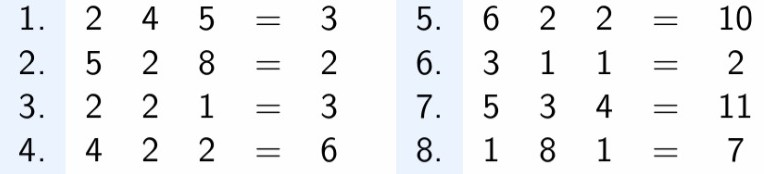
\includegraphics[scale=0.24]{chapter 3/ch3_figure1.jpeg}
    \end{wrapfigure}
    \raggedright
    Suppose we want to train our computer/machine to do maths.\\
    We pass a set of input data and the corresponding answers to the computer/machine and then ask it to learn/figure out the relationship between the data and the answers instead of explicitly programming it.\\
\end{egBox}
There are real-life applications of supervised learning:
\begin{enumerate}
    \item \textbf{Image Classification}: Classify images into different categories.\\
    \underline{\textbf{e.g.}}: Facebook recognizes our friend in a photo from an album of tagged photos.
    \vspace{1mm}
    \item \textbf{Visual Recognition}: Recognize objects in images.\\
    \underline{\textbf{e.g.}}: The ability of a machine to identify objects, places, people, actions and images.
    \vspace{1mm}
    \item \textbf{Signature Recognition}: Recognize signatures.\\
    \underline{\textbf{e.g.}}: Automatic signature recognition in banks.
    \vspace{1mm}
    \item \textbf{Spam Detection}: Detect spam emails.\\
    \underline{\textbf{e.g.}}: Gmail classifies emails as spam or not spam with 99.9\% accuracy.
    \vspace{1mm}
    \item \textbf{Weather Forecasting}: Predict weather conditions.\\
    \underline{\textbf{e.g.}}: HK Observatory incorporates machine learning in strengthening the techniques in monitoring and forecasting weather.
\end{enumerate}
\newpage
\subsection{Unsupervised Learning}
We use an \textcolor{cyan}{unlabelled dataset} without giving the correct outputs and train the machines to \textcolor{violet}{learn on their own}.\\
The computer/machine tries to \textcolor{violet}{find a pattern in the unlabelled data} and respond.\\
There are two types of unsupervised learning:
\begin{enumerate}
    \item \textcolor{cyan}{\textbf{Clustering}}: \textcolor{violet}{Group data into clusters} that are similar between them and are dissimilar to the objects belonging to another cluster.\\
    \underline{\textbf{e.g.}}: Find out which customers made similar product purchases.
    \item \textcolor{cyan}{\textbf{Association}}: A rule-based machine learning to \textcolor{violet}{discover the probability of the co-occurrence of items} in a collection.\\
    \underline{\textbf{e.g.}}: Finding our which products were purchased together.
\end{enumerate}
\begin{egBox}{Example 3.1.3}{}
    \begin{wrapfigure}[3]{r}{0.3\textwidth}
        \centering
        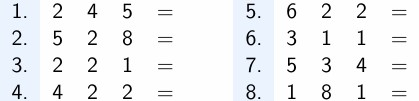
\includegraphics[scale=0.45]{chapter 3/ch3_figure2.jpeg}
    \end{wrapfigure}
    \raggedright
    Suppose we want to train our computer/machine to do maths.\\
    We pass a set of input data to the computer/machine without the corresponding answers to the computer/machine and then ask it to learn/figure out the pattern between the data and the answers instead of explicitly programming it.\\
\end{egBox}
There are real-life applications of unsupervised learning:
\begin{enumerate}
    \item \textbf{Semantic Clustering}\\
    \underline{\textbf{e.g.}}: Semantically similar words share a similar context, Grouping images/videos based on similarities \& Grouping audios based on acoustic similarity.
    \item \textbf{Identifying Accident Prone Areas}\\
    \underline{\textbf{e.g.}}: Used to identify accident-prone areas and introduce safety measures based on the itensity of accidents.
\end{enumerate}
\subsection{Comparison between Supervised and Unsupervised Learning}
\begin{center}
    \begin{tabular}{|m{2.9cm}|m{7.5cm}|m{6.5cm}|}
        \hline
        \rowcolor{lightblue}
        & \textbf{Supervised Learning} & \textbf{Unsupervised Learning} \\
        \hline
        \textbf{Training Data} & \textcolor{violet}{Labelled Data} & \textcolor{violet}{Unlabelled Data} \\
         & \textcolor{violet}{Need domain expert to label data} & \\
        \hline
        \textbf{Categories} & \textcolor{violet}{Classification \& Regression} & \textcolor{violet}{Clustering \& Association} \\
        \hline
        \textbf{Preference} & \textcolor{violet}{Calculate outcomes} & \textcolor{violet}{Discover underlying patterns} \\
        \hline
        \textbf{Training Time} & \textcolor{violet}{Shorter} & \textcolor{violet}{Longer} \\
        \hline
        \textbf{Accuracy} & \textcolor{violet}{Higher} & \textcolor{violet}{Lower} \\
        \hline
        \textbf{Optimal Strategy} & \textcolor{violet}{Depends on the data and learning algorithm} & \textcolor{violet}{Depends on the data} \\
        \hline
        & \textcolor{violet}{Naïve Bayes, K-Nearest Neighbours, Decision Tree, } & \textcolor{violet}{K-Means Clustering, Hierarchical Clustering, } \\
        \textbf{Algorithms} & \textcolor{violet}{Linear Regression, Logistics Regression, } & \textcolor{violet}{Apriori Algorithm, etc.} \\
        & \textcolor{violet}{Support Vector Machine, etc.} & \\
        \hline
    \end{tabular}
\end{center}
\textcolor{magenta}{\section{\textbf{Bayes' Rule}}}
\subsection{Conditional Probability}
\begin{thmBox}{Theorem 3.2.1}{Conditional Probability}
    \textcolor{purple}{Conditional probability} denoted by \(P(B|A)\) is the \textcolor{purple}{probability of event B occurring given that event A has already occurred}.
    \[
        P(B|A) = \frac{P(A \cap B)}{P(A)}
    \]
\end{thmBox}
\begin{egBox}{Example 3.2.1}{}
    \begin{center}
        \begin{tabular}{|m{2.5cm}|m{2.5cm}|m{2.5cm}|m{2.5cm}|}
             \hline
                        & \textbf{A} & \textbf{B} & \textbf{A $\cap$ B} \\
                        \hline
                        \textbf{Probability} & 0.3 & 0.4 & 0.2 \\
                        \hline
        \end{tabular}
    \end{center}
    Find the probability of B given A.
    \begin{align*}
        P(B|A) & = \frac{P(A \cap B)}{P(A)} = \frac{0.2}{0.3} = 0.67
    \end{align*}
\end{egBox}
\newpage
\subsection{Bayes' Rule}
\begin{thmBox}{Theorem 3.2.2}{Bayes' Rule}
    \textcolor{purple}{Bayes' Rule} is named after \textcolor{purple}{Thomas Bayes}, which is the most important rule in data science.\\
    $\Rightarrow$ A mathematical rule that \textcolor{purple}{describes how to update a belief given some evidence}.
        \[
            P(B|E) = \frac{P(B) \cdot P(E|B)}{P(E)} = \frac{P(B) \cdot P(E|B)}{P(B) \cdot P(E|B) + P(B') \cdot P(E|B')}
        \]
        \raggedright
        where:\\
        \textcolor{brown}{\(E\)}: Evidence/Feature\\
        \textcolor{brown}{\(B\)}: Belief/Class\\
        \textcolor{brown}{\(P(B|E)\)}: Posterior Probability (Probability of belief occurss given evidence has occurred)\\
        \textcolor{brown}{\(P(B)\)}: Prior Probability (Probability of belief happens)\\
        \textcolor{brown}{\(P(E|B)\)}: Likelihood (Probability of evidence occurs given belief has occurred)\\
        \textcolor{brown}{\(P(E)\)}: Marginal Probability (Probability of evidence occurs)\\
        \textcolor{brown}{\(P(B')\)}: Complement of B (Probability of belief does not happen)\\
        \textcolor{brown}{\(P(E|B')\)}: Likelihood of B' (Probability of evidence occurs given belief does not happen)
\end{thmBox}
In other words, Bayes' Rule gives us the \textcolor{violet}{conditional probability of a belief B given some evidence E has occured} as long as we know \(P(E|B)\), \(P(E|B')\), \(P(B)=1-P(B')\).\\
\begin{figure}[h]
    \centering
    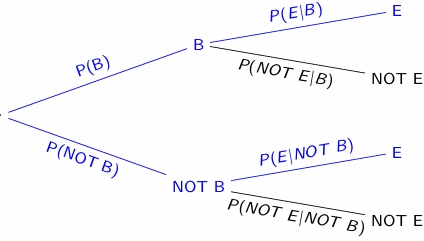
\includegraphics[scale=0.7]{chapter 3/ch3_figure3.jpeg}
    \caption{Tree Diagram of Bayes' Rule}
\end{figure}
\textbf{\large{\textit{Proof:}}}\\
By the definition of conditional probability, we have: 
\[
P(E|B) = \frac{P(E \cap B)}{P(B)} .\tag{1}
\]
\[
P(E \cap B) = P(E|B) \cdot P(B) .\tag{2}
\]
By the law of total probability, we have: 
\[
P(E) = P((E \cap B) \cup (E \cap B')) = P(E \cap B) + P(E \cap B') .\tag{3}
\]
By substituting equation (2) into equation (3), we have:
\[
P(E) = P(E|B) \cdot P(B) + P(E|B') \cdot P(B') .\tag{4}
\]
where on Equation (4), \(E \cap B\) and \(E \cap B'\) are mutually exclusive.\\
Since \(E \cap B = B \cap E\), by Equations (1) and (2), we have:
\[
P(B|E) = \frac{B \cap E}{P(E)} = \frac{P(E|B) \cdot P(B)}{P(E)}.\tag{5}
\]
By substituting Equation (4) into Equation (5), we have:
\[
P(B|E) = \frac{P(E|B) \cdot P(B)}{P(E|B) \cdot P(B) + P(E|B') \cdot P(B')} .\tag{6}
\]
\newpage
\begin{egBox}{Example 3.2.2}{Virus Detection}
    \raggedright
    \textbf{Question}: \\
    A doctor gives a patient a test for a particular virus. It is believed that 0.1\% of the population has the virus. Based on experience, the doctor knows that, in 99\% of the cases, the test will be positive if the patient has the virus and in 95\% of the cases, the test will be negative if the patient does not have the virus.\\
    If the test turns out to be positive, what is the probability that the patient has the virus?\\
    \vspace{2mm}
    \textbf{Answer}: \\
    Let \(V\) be the event that the patient has the virus and \(H\) be the event that the patient does not have the virus.\\
    Let \(P(V) = 0.001\), \(P(H) = 1-0.001 = 0.999\), \(P(+|V) = 0.99\), \(P(-|H) = 0.95\).\\
    According to Bayes' Rule, we have:
    \[
        P(V|+) = \frac{P(V) \cdot P(+|V)}{P(+)} = \frac{P(V) \cdot P(+|V)}{P(V) \cdot P(+|V) + P(H) \cdot P(+|H)}
    \]
    Then we find the probability of the test being positive:
    \[
        P(+) = P(V) \cdot P(+|V) + P(H) \cdot P(+|H) = 0.001 \cdot 0.99 + 0.999 \cdot 0.05 = 0.05095
    \]
    Finally, we find the probability of the patient having the virus given that the test is positive:
    \[
        P(V|+) = \frac{0.001 \cdot 0.99}{0.001 \cdot 0.99 + 0.999 \cdot 0.05} = \frac{0.00099}{0.00099 + 0.04995} = \frac{0.00099}{0.05094} = 0.0194
    \]
    $\therefore$ The probability that the patient has the virus given that the test is positive is 0.0194.
\end{egBox}
\subsection{General Forrm of Bayes' Rule}
\begin{thmBox}{Theorem 3.2.3}{General Form of Bayes' Rule}
    \textcolor{purple}{Bayes' Rule} can be written in a more general form as:
    \[
        P(B_i|E) = \frac{P(B_i) \cdot P(E|B_i)}{P(E|B_1) \cdot P(B_1) + P(E|B_2) \cdot P(B_2) + \ldots + P(E|B_n) \cdot P(B_n)}
        = \frac{P(B_i) \cdot P(E|B_i)}{\sum_{j=1}^{n} P(E|B_j) \cdot P(B_j)}
    \]
    \raggedright
    where:
    \begin{description}
        \item[\textcolor{brown}{\(B_i\)}]: Each Belief/Class
        \item[\textcolor{brown}{\(E\)}]: Evidence/Feature
    \end{description}
\end{thmBox}
In other words, \(B_1, B_2, \ldots, B_n\) are the different classes of the belief and \(P(B_i|E)\) is the probability of the belief \(B_i\) given the evidence \(E\).
\begin{figure}[h]
    \centering
    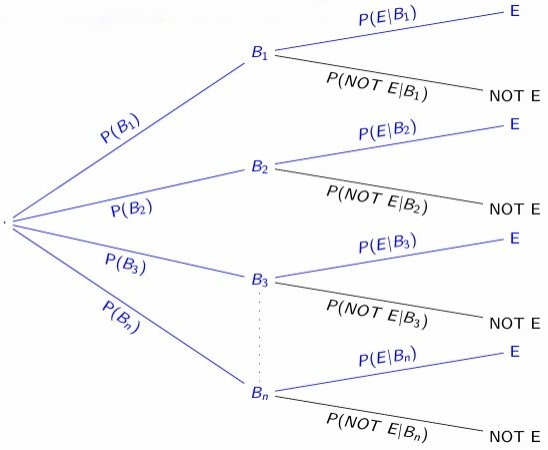
\includegraphics[scale=0.7]{chapter 3/ch3_figure4.jpeg}
    \caption{Tree Diagram of General Form of Bayes' Rule}
\end{figure}
\newpage
\textcolor{magenta}{\section{\textbf{Naïve Bayes Classifier}}}
\subsection{Introduction to Naïve Bayes Classifier}
\begin{defBox}{Definition 3.3.1}{Naïve Bayes Classifier}
    \textcolor{cyan}{Naïve Bayes Classifier} is a \textcolor{cyan}{probabilistic classifier} based on \textcolor{cyan}{Bayes' Rule} when we assume that \textcolor{cyan}{each piece of evidence is independent of the others and equally contributes} to the probability of a sample belonging to a particular belief/class. \\
    $\Rightarrow$ The presence of a particular evidence in a belief is unrelated to the presence of any other evidence.
\end{defBox}
Assumptions of Naïve Bayes Classifier:
\begin{enumerate}
    \item \textcolor{cyan}{\textbf{Independence}}: The features are assumed to be independent of each other, meaning the presence of one feature does not affect the presence of another feature.
    \item \textcolor{cyan}{\textbf{Equal Contribution}}: Each feature contributes equally to the probability of a outcome.
\end{enumerate}
However, the assumptions made by Naïve Bayes Classifier are \textcolor{violet}{NOT correct in real-life scenarios}. But, the independence assumption \textcolor{violet}{still works well in practice}.\\
\vspace{1mm}
With each evidence makes an independent and equal contribution given the belief, the probability of a belief given the evidence can be calculated as:
\[
    P(B_i|E) = \frac{P(B_i) \cdot P((e_1, e_2, \ldots, e_d|B_i)}{\sum_{j=1}^{n} P(B_j) \cdot P((e_1, e_2, \ldots, e_d|B_j)} = \frac{P(B_i) \cdot P(e_1|B_i) \cdot P(e_2|B_i) \cdot \ldots \cdot P(e_d|B_i)}{\sum_{j=1}^{n} P(B_j) \cdot P(e_1|B_j) \cdot P(e_2|B_j) \cdot \ldots \cdot P(e_d|B_j)}
\]
\begin{thmBox}{Theorem 3.3.1}{Naïve Bayes Classifier}
    Suppose we assume that we are interested in \textcolor{purple}{knowing which belief has the highest probability value rather than the actual probability value}.\\
    Then, the \textcolor{purple}{Naïve Bayes Classifier} can be written as:
    \[
        B_{NB} = argmax_{B_i} P(B_i) \cdot P(e_1|B_i) \cdot P(e_2|B_i) \cdot \ldots \cdot P(e_d|B_i)
    \]
    where:
    \begin{description}
        \item[\textcolor{brown}{\(B_{NB}\)}]: Naïve Bayes Classifier
        \item[\textcolor{brown}{\(B_i\)}]: Each Belief/Class
        \item[\textcolor{brown}{\(e_1, e_2, \ldots, e_d\)}]: Features/Evidence
    \end{description}
    \vspace{1mm}
    The denominator of the Naïve Bayes Classifier is removed since it is a constant value and does not affect the outcome.
\end{thmBox}
\subsection{Zero Frequency Problem and \(\alpha\)-Laplace Smoothing}
\textcolor{olive}{\subsubsection{Zero Frequency Problem}}
\begin{defBox}{Definition 3.3.2.1}{\textcolor{cyan}{Zero Frequency Problem}}
If the categorial variable has a category in the test data set, which was \textcolor{red}{not observed in training data set}, then \textcolor{blue}{the model will assign a zero probability} and will be unable to make a prediction.
\end{defBox}
\textcolor{olive}{\subsubsection{\(\alpha\)-Laplace Smoothing (Solution)}}
\begin{defBox}{Definition 3.3.2.2}{\textcolor{cyan}{\(\alpha\)-Laplace Smoothing}}
\raggedright
Pretend that we have seen every evidence given every belief \(\alpha\) more times than we actually have.\\
\[
    P(e_j = v_j|B_i = c_i) = \frac{Count(e_j = v_j \cap B_i = c_i) + \alpha}{Count(B_i = c_i) + \alpha \cdot |V_j|}
\]
where \(n\) is the number of possible values of the evidence \(e_j\).\\
\vspace{1.5mm}
$\therefore$ \textcolor{cyan}{\textbf{\(\alpha = 1\) or 1-Laplace Smoothing}: Pretend that we have seen 1 more time we actually did.}
\end{defBox}
\newpage
\subsection{Naïve Bayes Classifier in Practice}
We can use the Naïve Bayes Classifier to classify the data into different classes based on the features in discrete variables and continuous variables.\\
\vspace{2mm}
\underline{\textbf{Example 1: Discrete Variables Calculation}}\\
Suppose we have a dataset with the following features and classes:
\begin{center}
    \begin{tabular}{|m{1cm}|m{2.5cm}|m{1.5cm}|m{1.5cm}|m{1cm}|m{4cm}|}
        \hline
        \rowcolor{lightblue}
        \textbf{Data} & \textbf{Blood Pressure} & \textbf{Fever} & \textbf{Diabetes} & \textbf{Vomit} & \textbf{Suffering from disease Z} \\
        \hline
        1 & High & High & Yes & No & No \\
        \hline
        2 & High & High & Yes & Yes & No \\
        \hline
        3 & Low & High & Yes & No & Yes \\
        \hline
        4 & Normal & Mild & Yes & No & Yes \\
        \hline
        5 & Normal & No Fever & No & No & Yes \\
        \hline
        6 & Normal & No Fever & No & Yes & No \\
        \hline
        7 & Low & No Fever & No & Yes & Yes \\
        \hline
        8 & High & Mild & Yes & No & No \\
        \hline
        9 & High & No Fever & No & No & Yes \\
        \hline
        10 & Normal & Mild & No & No & Yes \\
        \hline
        11 & High & Mild & No & Yes & Yes \\
        \hline
        12 & Low & Mild & Yes & Yes & Yes \\
        \hline
        13 & Low & High & No & No & Yes \\
        \hline
        14 & Normal & Mild & Yes & Yes & No \\
        \hline
    \end{tabular}
\end{center}
Suppose we want to find the probability of a patient suffering from disease Z given the symptoms (High, No Fever, Yes, Yes).\\
\vspace{1mm}
Relative Frequency of the classes:
\resizebox{\textwidth}{!}{
    \begin{tabular}{|m{1.5cm}|m{0.5cm}|m{0.5cm}||m{1.5cm}|m{0.5cm}|m{0.5cm}||m{1.5cm}|m{0.5cm}|m{0.5cm}||m{1.5cm}|m{0.5cm}|m{0.5cm}||m{1.5cm}|m{0.5cm}|}
        \hline
        \rowcolor{lightblue}
        \multicolumn{3}{|c|}{\textbf{Blood Pressure}} & \multicolumn{3}{c|}{\textbf{Fever}} & \multicolumn{3}{c|}{\textbf{Diabetes}} & \multicolumn{3}{c|}{\textbf{Vomit}} & \multicolumn{2}{c|}{\textbf{Suffering from disease Z}} \\
        \hline
        & Yes & No & & Yes & No & & Yes & No & & Yes & No & Yes & No \\
        \hline
        \vspace{1mm}
        High & \(\frac{2}{9}\) & \(\frac{3}{5}\) & High & \(\frac{2}{9}\) & \(\frac{2}{5}\) & Yes & \(\frac{3}{9}\) & \(\frac{4}{5}\) & Yes & \(\frac{3}{9}\) & \(\frac{3}{5}\) & \(\frac{9}{14}\) & \(\frac{5}{14}\) \\
        \hline
        \vspace{1mm}
        Normal & \(\frac{3}{9}\) & \(\frac{2}{5}\) & Mild & \(\frac{4}{9}\) & \(\frac{2}{5}\) & No & \(\frac{6}{9}\) & \(\frac{1}{5}\) & No & \(\frac{6}{9}\) & \(\frac{2}{5}\) & & \\
        \hline
        \vspace{1mm}
        Low & \(\frac{4}{9}\) & \(\frac{0}{5}\) & No Fever & \(\frac{3}{9}\) & \(\frac{1}{5}\) & & & & & & & & \\
        \hline
    \end{tabular}
}
\vspace{1mm}
Given the Naïve Bayes' Classifier Formula \(P(B_{NB}) = argmax_{B_i} P(B_i) \cdot P(e_1|B_i) \cdot P(e_2|B_i) \cdot P(e_3|B_i) \ldots P(e_d|B_i)\), we have:

\begin{align*}
    & P(\text{Disease Z = Yes}) \cdot P(\text{BP = High}|\text{Z = Yes}) \cdot P(\text{Fever = No}|\text{Z = Yes}) \cdot P(\text{Diabetes = Yes}|\text{Z = Yes}) \cdot P(\text{Vomit = Yes}|\text{Z = Yes}) \\
    & = \frac{9}{14} \cdot \frac{2}{9} \cdot \frac{3}{9} \cdot \frac{3}{9} \cdot \frac{3}{9} = 0.0052910053\ldots = \underline{\underline{\frac{1}{189}}} 
\end{align*}
\begin{align*}
    & P(\text{Disease Z = No}) \cdot P(\text{BP = High}|\text{Z = No}) \cdot P(\text{Fever = No}|\text{Z = No}) \cdot P(\text{Diabetes = Yes}|\text{Z = No}) \cdot P(\text{Vomit = Yes}|\text{Z = No}) \\
    & = \frac{5}{14} \cdot \frac{3}{5} \cdot \frac{1}{5} \cdot \frac{4}{5} \cdot \frac{3}{5} = 0.0205714285\ldots = \underline{\underline{\frac{18}{875}}}
\end{align*}

$\therefore$ Since \(\frac{1}{189} < \frac{18}{875}\), the patient is \textcolor{red}{not suffering from disease Z}.\\
After normalization, we have:
\[
    P(\text{Disease Z = No}) = \frac{\frac{18}{875}}{\frac{1}{189} + \frac{18}{875}} = \underline{\underline{0.795414121\ldots}} \quad \text{and} \quad P(\text{Disease Z = Yes}) = \frac{\frac{1}{875}}{\frac{1}{189} + \frac{18}{875}} = \underline{\underline{0.204585878\ldots}}
\]\\
\newpage
\textit{\large{Naïve Bayes Classifier Python Code implementation using Scikit-Learn:}}
\begin{lstlisting}[language=Python, basicstyle=\ttfamily\small, keywordstyle=\color{blue}, commentstyle=\color{forestgreen}, stringstyle=\color{red}]
import numpy as np
# CategoricalNB is used for doing Naive Bayes Classifier for categorial features
from sklearn.naive_bayes import CategoricalNB

# Forming training data
# Features: Blood Pressure (0 = High, 1 = Normal, 2 = Low), Fever (0 = High, 1 = Mild, 2 = No Fever), 
#           Diabetes (0 = Yes, 1 = No), Vomit (0 = Yes, 1 = No)
training = np.array([[0, 0, 0, 1], [0, 0, 0, 0], [2, 0, 0, 1], [1, 1, 0, 1], [1, 2, 1, 1], 
                     [1, 2, 1, 0], [2, 2, 1, 0], [0, 1, 0, 1], [0, 2, 1, 1], [1, 1, 1, 1], 
                     [0, 1, 1, 0], [2, 1, 0, 0], [2, 0, 1, 1], [1, 1, 0, 0]])

# Forming the label set
# Labels: Suffering from disease Z (0 = Yes, 1 = No)
outcome = np.array([1, 1, 0, 0, 0, 1, 0, 1, 0, 0, 0, 0, 0, 1])

# New data to be evaluated using the trained AI module
new_sample = np.array([[0, 2, 0, 0]])

# Train Naive Bayes Classifier according to training, outcome
clf = CategoricalNB(alpha=1.0e-10).fit(training, outcome)

# Perform classification on new_sample and get the probability estimated
pred_class = clf.predict(new_sample)
pred_prob = clf.predict_proba(new_sample)
# Print the results
print(pred_class, pred_prob)

# Output: [1] [[0.20458265 0.79541735]]
\end{lstlisting}
\newpage
\underline{\textbf{Example 2: Continuous Variables Calculation}}\\
Assume the \textcolor{cyan}{probability of likelihood} follows the \textcolor{cyan}{Gaussian Distribution}:
\begin{wrapfigure}[6]{r}{0.35\textwidth}
    \centering
    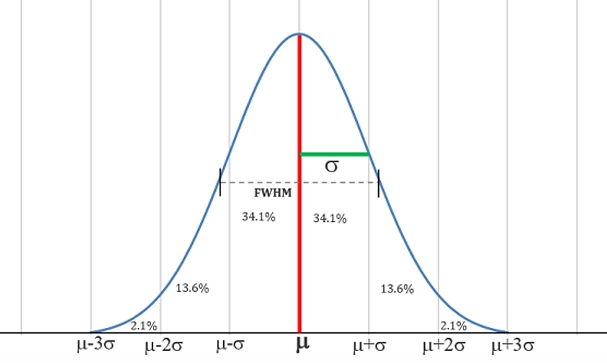
\includegraphics[scale=0.32]{chapter 3/ch3_figure5.jpeg}
\end{wrapfigure}
\[
    f(x) = \frac{1}{\sqrt{2\pi\sigma^2}} \cdot e^{-\frac{(x-\mu)^2}{2\sigma^2}}
\]
where:\\
\textcolor{brown}{\(f(x)\)}: Gaussian Distribution Function\\
\textcolor{brown}{\(\mu\)}: Mean of the distribution\\
\textcolor{brown}{\(\sigma\)}: Standard Deviation of the distribution\\
\textcolor{brown}{\(x\)}: Value of the variable\\
\vspace{1.5cm}
If the Blood Pressure and Fever are continuous, we need to calculate the mean and standard deviation of Blood Pressure and Fever for each belief.\\
Suppose for Blood Pressure:
\begin{description}
    \centering
    \item[$\bullet$] Suffering from Disease Z is Yes: \(\mu = 73\), \(\sigma = 6.2\)
    \item[$\bullet$] Suffering from Disease Z is No: \(\mu = 75\), \(\sigma = 7.9\)
\end{description}
Suppose for Fever:
\begin{description}
    \centering
    \item[$\bullet$] Suffering from Disease Z is Yes: \(\mu = 79\), \(\sigma = 10.2\)
    \item[$\bullet$] Suffering from Disease Z is No: \(\mu = 86\), \(\sigma = 9.7\)
\end{description}
\vspace{1mm}
When Blood Pressure = 66:\\
\[
    P(\text{Blood Pressure = 66}|\text{Z = Yes}) = \frac{1}{\sqrt{2\pi \cdot 6.2^2}} \cdot e^{-\frac{(66-73)^2}{2 \cdot 6.2^2}} = 0.0340187\ldots
\]
\[
    P(\text{Blood Pressure = 66}|\text{Z = No}) = \frac{1}{\sqrt{2\pi \cdot 7.9^2}} \cdot e^{-\frac{(66-75)^2}{2 \cdot 7.9^2}} = 0.0263909\ldots
\]
When Fever = 97:\\
\[
    P(\text{Fever = 97}|\text{Z = Yes}) = \frac{1}{\sqrt{2\pi \cdot 10.2^2}} \cdot e^{-\frac{(97-79)^2}{2 \cdot 10.2^2}} = 0.00824276\ldots
\]
\[
    P(\text{Fever = 97}|\text{Z = No}) = \frac{1}{\sqrt{2\pi \cdot 9.7^2}} \cdot e^{-\frac{(97-86)^2}{2 \cdot 9.7^2}} = 0.0216215\ldots
\]
Posterior Probability Calculation:\\
\begin{align*}
    & P(\text{Disease Z = Yes}) \cdot P(\text{Blood Pressure = 66}|\text{Z = Yes}) \cdot P(\text{Fever = 97}|\text{Z = Yes}) \cdot P(\text{Diabetes = Yes}|\text{Z = Yes}) \cdot P(\text{Vomit = Yes}|\text{Z = Yes}) \\
    & = \frac{9}{14} \cdot 0.0340187 \cdot 0.00824276 \cdot \frac{3}{9} \cdot \frac{3}{9} = \underline{\underline{0.00002}}
\end{align*}
\begin{align*}
    & P(\text{Disease Z = No}) \cdot P(\text{Blood Pressure = 66}|\text{Z = No}) \cdot P(\text{Fever = 97}|\text{Z = No}) \cdot P(\text{Diabetes = Yes}|\text{Z = No}) \cdot P(\text{Vomit = Yes}|\text{Z = No}) \\
    & = \frac{5}{14} \cdot 0.0263909 \cdot 0.0216215 \cdot \frac{4}{5} \cdot \frac{3}{5} = \underline{\underline{0.0000978}}
\end{align*}
$\therefore$ Since \(0.00002 < 0.0000978\), the patient is \textcolor{red}{not suffering from disease Z}.\\
After normalization, we have:
\[
    P(\text{Disease Z = No}) = \frac{0.0000978}{0.00002 + 0.0000978} = \underline{\underline{0.8302207\ldots}} \quad \text{and} \quad P(\text{Disease Z = Yes}) = \frac{0.00002}{0.00002 + 0.0000978} = \underline{\underline{0.1697793\ldots}}
\]
\newpage
\textbf{\large{\textit{Remark:}}}\\
In \textcolor{cyan}{continuous variables}, \textcolor{violet}{the probability of getting precisely any given outcome is 0}, and hence densities are used.\\
We deal with the \textcolor{cyan}{probability of X being close to x: \(P(X - x | < \triangle(x))\)}.\\
Applying the Bayes' Rule, we get:
\[
    P(X \approx x|W \approx w) = \frac{P(X \approx x) \cdot P(W \approx w|X \approx x)}{P(W \approx w)}
\]
Substituting the density function, we get:
\[
    pdf(x|w)\triangle(x) = \frac{pdf(w|x)\triangle(w)\cdot pdf(x)\triangle(x)}{pdf(w)\triangle(w)}
\]
Since \(Probability = Density \times NeighbourhoodSize\), we get the \textcolor{cyan}{Bayes Rule for Densities}:
\[
    pdf(x|w) = \frac{pdf(w|x) \cdot pdf(x)}{pdf(w)}
\]
For \textcolor{cyan}{integral approximations}, to get the probability of a specific variable value from the variable's continuous PDF (Probability Density Function), we \textcolor{violet}{integrate the PDF around the value in question over an interval of width epsilon} and \textcolor{violet}{take the limit of that integral as epsilon approaches 0}.\\
For \textcolor{cyan}{small epsilon}, the integral \textcolor{violet}{will be equivalent to the product of epsilon and the PDF at the variable value in question}.\\
In Naïve Bayes Classifier, we are interested in the ratio of conditional probabilities, so these factors of epsilon will cancel out from the numerator and denominator.\\
The limit of the ratio of the conditional probabilities will be the ratio of the PDF heights at the variable value in question.\\
\vspace{2mm}
\textcolor{red}{$\therefore$ Given the Bayes' Rule also holds for densities, we can use the same methods replacing probabilities with densities when dealing with continuous variables.}\\

\subsection{Underflow Prevention in Naïve Bayes Classifier}
\textcolor{cyan}{Floating-point underflow} occurs when we multiply lots of probability between 0 and 1, \textcolor{purple}{the result becomes too small to be represented by the computer}.\\
To prevent underflow, we can use the \textcolor{cyan}{logarithm} of the probabilities.\\
\(log(x \cdot y) = log(x) + log(y)\) can perform all computations by \hl{summing logs of probabilities instead of multiplying} probabilities.\\
Belief with the highest probability is the same as the belief with the highest log probability.\\
\begin{thmBox}{Theorem 3.3.4}{Logarithm of Probabilities in Naïve Bayes Classifier}
    \raggedright
    To prevent underflow in Naïve Bayes Classifier, we can use the logarithm of the probabilities.\\
    \[
        B_{NB} = argmax_{B_i} (log(P(B_i)) + \sum_(n=1)^d log(P(e_n|B_i)))
    \]
    where:
    \begin{description}
        \item[\textcolor{brown}{\(B_{NB}\)}]: Naïve Bayes Classifier
        \item[\textcolor{brown}{\(B_i\)}]: Each Belief/Class
        \item[\textcolor{brown}{\(e_n\)}]: Each Evidence/Feature
    \end{description}
\end{thmBox}
\fbox{
    \parbox{0.95\textwidth}{
        \textcolor{cyan}{\textbf{Note}}: The logarithm we use is \hl{Natural Logarithm} (base \(e\)).
    }
}\\


\newpage
\subsection{Applications of Naïve Bayes Classifier}
\begin{description}
    \item[$\bullet$] \textcolor{cyan}{\textbf{Real-time Prediction}}:\\
    Naïve Bayes Classifier is an extremely \textcolor{violet}{fast} and always ready to learn, which is suitable for real-time predictions.
    \item[$\bullet$] \textcolor{cyan}{\textbf{Multi-class Prediction}}:\\
    Naïve Bayes Classifier can predict the probability of multiple classes of any target variable.
    \item[$\bullet$] \textcolor{cyan}{\textbf{Text Classification/Spam Filtering/Sentiment Analysis}}:\\
    Naïve Bayes Classifier performs better or have a higher accuracy in text classification tasks due to its better performance with multi-class problems and independence assumption.
    \item[$\bullet$] \textcolor{cyan}{\textbf{Recommendation System}}:\\
    Naïve Bayes Classifier can be used to build a recommendation system that uses machine learning and data mining techniques to filter unseen information and predict whether a user would like a given resource or not with collaborative filtering.
\end{description}
\subsection{Advantages and Disadvantages of Naïve Bayes Classifier}
\textcolor{olive}{\subsubsection{Advantages}}
\begin{description}
    \item[$\bullet$] \textcolor{cyan}{\textbf{Easy to Implement}}:\\
    \textcolor{violet}{Very easy to implement} and obtain good results on large datasets.
    \item[$\bullet$] \textcolor{cyan}{\textbf{Computational Efficiency}}:\\
    The assumption that all features are independent of each other makes the computation very fast compared to complicated algorithms.
    \item[$\bullet$] \textcolor{cyan}{\textbf{Good performance on Large Datasets}}:\\
    \textcolor{violet}{Works} well on a \textcolor{violet}{large size dataset}.
    \item[$\bullet$] \textcolor{cyan}{\textbf{Multi-class Prediction}}.
    \item[$\bullet$] \textcolor{cyan}{\textbf{Natural Language Processing Text Classification}}.
\end{description}
\textcolor{olive}{\subsubsection{Disadvantages}}
\begin{description}
    \item[$\bullet$] \textcolor{red}{\textbf{Assumption of Independence}}:\\
    The strong assumption that all features are \textcolor{violet}{independent} of each other is \textcolor{red}{not correct in real-life scenarios}.\\
    $\implies$ \hl{Not suitable for regression problems} and \textcolor{violet}{not suitable for continuous variables}.
    \item[$\bullet$] \textcolor{red}{\textbf{Precision Problem}}:\\
    If the dataset is \textcolor{violet}{small}, it will \hl{decrease the precision value} of the model.
    \item[$\bullet$] \textcolor{red}{\textbf{Biased Outcome}}:\\
    If the goal is to predict the probability of a belief/class, then Naïve Bayes Classifier will be \textcolor{violet}{biased}.
    \item[$\bullet$] \textcolor{red}{\textbf{Zero Frequency Problem}}:\\
    If a categorial variable has a category in the test data set, which was not observed in the training data set, then the model will assign a zero probability and will be unable to make a prediction.
\end{description}
\newpage
\textbf{\textcolor{purple}{\Large{Practice Problems}}}\\
\vspace{1mm}
\underline{\textbf{Problem 1}}\\
\textbf{Question:}
\begin{center}
    \begin{tabular}{|m{1cm}|m{2cm}|m{1.5cm}|m{1.5cm}|m{4cm}|}
        \hline
        \rowcolor{lightblue}
        \textbf{Data} & \textbf{Animals} & \textbf{Size} & \textbf{Colour} & \textbf{Can we pet the animal?} \\
        \hline
        1 & Dog & Medium & Black & Yes \\
        \hline
        2 & Dog & Big & White & No \\
        \hline
        3 & Rat & Small & White & Yes \\
        \hline
        4 & Cow & Big & White & Yes \\
        \hline
        5 & Cow & Small & Brown & No \\
        \hline
        6 & Cow & Big & Black & Yes \\
        \hline
        7 & Rat & Big & Brown & No \\
        \hline
        8 & Dog & Small & Brown & Yes \\
        \hline
        9 & Dog & Medium & Brown & Yes \\
        \hline
        10 & Cow & Medium & White & No \\
        \hline
        11 & Dog & Small & Black & Yes \\
        \hline
        12 & Rat & Medium & Black & No \\
        \hline
        13 & Rat & Small & Brown & No \\
        \hline
        14 & Cow & Big & White & Yes \\
        \hline
    \end{tabular}
\end{center}
For the animal (Animals = Cow, Size = Medium, Colour = Black), can we pet the animal?\\
\vspace{2mm}
\textbf{Answer:}\\
Given the Naïve Bayes Classifier Formula \(P(B_{NB}) = argmax_{B_i} P(B_i) \cdot P(e_1|B_i) \cdot P(e_2|B_i) \cdot P(e_3|B_i) \ldots P(e_d|B_i)\), we have:
\begin{align*}
    & P({\text{Pet = Yes}}) \cdot P({\text{Animals = Cow}}|{\text{Pet = Yes}}) \cdot P({\text{Size = Medium}}|{\text{Pet = Yes}}) \cdot P({\text{Colour = Black}}|{\text{Pet = Yes}}) \\
    & = \frac{8}{14} \cdot \frac{3}{8} \cdot \frac{2}{8} \cdot \frac{3}{8} = 0.020089285\ldots = \underline{\underline{\frac{9}{448}}}
\end{align*}
\begin{align*}
    & P({\text{Pet = No}}) \cdot P({\text{Animals = Cow}}|{\text{Pet = No}}) \cdot P({\text{Size = Medium}}|{\text{Pet = No}}) \cdot P({\text{Colour = Black}}|{\text{Pet = No}}) \\
    & = \frac{6}{14} \cdot \frac{2}{6} \cdot \frac{2}{6} \cdot \frac{1}{6} = 0.0079365079\ldots = \underline{\underline{\frac{1}{126}}}
\end{align*}
$\therefore$ Since \(\frac{9}{448} > \frac{1}{126}\), we can \textcolor{red}{pet the animal}.\\
After normalization, we have:
\[
    P({\text{Pet = Yes}}) = \frac{\frac{9}{448}}{\frac{9}{448} + \frac{1}{126}} = \underline{\underline{0.7168459\ldots}} \quad \text{and} \quad P({\text{Pet = No}}) = \frac{\frac{1}{126}}{\frac{9}{448} + \frac{1}{126}} = \underline{\underline{0.2831541\ldots}}
\]\\
\textit{\large{Naïve Bayes Classifier Python Code implementation using Scikit-Learn:}}
\begin{lstlisting}[language=Python, basicstyle=\ttfamily\small, keywordstyle=\color{blue}, commentstyle=\color{forestgreen}, stringstyle=\color{red}]
import numpy as np
# CategoricalNB is used for doing Naive Bayes Classifier for categorial features
from sklearn.naive_bayes import CategoricalNB

# Forming training data
# Features: Animals (0 = Dog, 1 = Rat, 2 = Cow), Size (0 = Big, 1 = Medium, 2 = Small),
#           Colour (0 = Black, 1 = White, 2 = Brown)
training = np.array([[0, 1, 0], [0, 0, 1], [1, 2, 1], [2, 0, 1], [2, 2, 2],
                     [2, 0, 0], [1, 0, 2], [0, 2, 2], [0, 1, 2], [2, 1, 1],
                     [0, 2, 0], [1, 1, 0], [1, 2, 2], [2, 0, 1]])

# Forming the label set
# Labels: Can we pet the animal? (0 = Yes, 1 = No)
outcome = np.array([0, 1, 0, 0, 1, 0, 1, 0, 0, 1, 0, 1, 1, 0])

# New data to be evaluated using the trained AI module
new_sample = np.array([[2, 1, 0]])

# Train Naive Bayes Classifier according to training, outcome
clf = CategoricalNB(alpha=1.0e-10).fit(training, outcome)
# Perform classification on new_sample and get the probability estimated
pred_class = clf.predict(new_sample)
pred_prob = clf.predict_proba(new_sample)
# Print the results
print(pred_class, pred_prob)

# Output: [0] [[0.71681416 0.28318584]]
\end{lstlisting}
\newpage
\underline{\textbf{Problem 2}}\\
\begin{center}
    \begin{tabular}{|c|c|c|c|}
        \hline
        \rowcolor{lightblue}
        \textbf{Gender} & \textbf{Age Group} & \textbf{Martial Status} & \textbf{Purchased} \\
        \hline
        Male & Youth & Single & Yes \\
        \hline
        Female & Adult & Married & Yes \\
        \hline
        Male & Adult & Single & No \\
        \hline
        Female & Senior & Married & No \\
        \hline
        Male & Senior & Married & Yes \\
        \hline
        Female & Youth & Single & Yes \\
        \hline
        Male & Adult & Married & No \\
        \hline
        Female & Adult & Single & Yes \\
        \hline
    \end{tabular}
\end{center}
\textbf{Question 2.1:} Calculate the prior probabilities for each class (Purchased = Yes and Purchased = No).\\
\textbf{Answer:}\\
Count the total number of instances for each class: \textcolor{gray}{\(\text{Total Instances} = 8\)}.\\
Count the numbers of instances for each class: \textcolor{gray}{\(\text{(Purchased = Yes)} = 5\)} and \textcolor{gray}{\(\text{(Purchased =No)} = 3\)}.\\
Calculate the prior probabilities for each class:
\[
    P(\text{Purchased = Yes}) = \frac{5}{8} = \underline{\underline{0.625}} \quad \text{and} \quad P(\text{Purchased = No}) = \frac{3}{8} = \underline{\underline{0.375}}
\]
\textbf{Question 2.2:} Using Laplace Smoothing (\(\alpha = 1\)), compute the likelihood of the following instance: Gender = Female, Age Group = Senior,  Martial Status = Married.\\
\textbf{Answer:}\\
For Purchased = Yes:
\[
    P(\text{Female}|\text{Purchased = Yes}) = \frac{3 + 1}{5 + 2} = \frac{4}{7} = \underline{\underline{0.5714285}}
\]
\[
    P(\text{Senior}|\text{Purchased = Yes}) = \frac{1 + 1}{5 + 3} = \frac{2}{8} = \underline{\underline{0.25}}
\]
\[
    P(\text{Married}|\text{Purchased = Yes}) = \frac{2 + 1}{5 + 2} = \frac{3}{7} = \underline{\underline{0.4285714}}
\]
For Purchased = No:
\[
    P(\text{Female}|Purchased = No) = \frac{1 + 1}{3 + 2} = \frac{2}{5} = \underline{\underline{0.4}}
\]
\[
    P(\text{Senior}|Purchased = No) = \frac{1 + 1}{3 + 3} = \frac{2}{6} = \underline{\underline{0.3333333}}
\]
\[
    P(\text{Married}|Purchased = No) = \frac{2 + 1}{3 + 2} = \frac{3}{5} = \underline{\underline{0.6}}
\]
\textbf{Question 2.3:} What is the predicted class for this instance using the Naïve Bayes Classifier?\\
\textbf{Answer:}\\
Given the Naïve Bayes Classifier Formula \(P(B_{NB}) = argmax_{B_i} P(B_i) \cdot P(e_1|B_i) \cdot P(e_2|B_i) \cdot P(e_3|B_i) \ldots P(e_d|B_i)\), we have:
\begin{align*}
    & P(\text{Purchased = Yes}) \cdot P(\text{Female}|\text{Purchased = Yes}) \cdot P(\text{Senior}|\text{Purchased = Yes}) \cdot P(\text{Married}|\text{Purchased = Yes}) \\
    & = 0.625 \cdot 0.5714285 \cdot 0.25 \cdot 0.4285714 = 0.0826530612\ldots = \underline{\underline{\frac{15}{392}}}
\end{align*}
\begin{align*}
    & P(\text{Purchased = No}) \cdot P(\text{Female}|\text{Purchased = No}) \cdot P(\text{Senior}|\text{Purchased = No}) \cdot P(\text{Married}|\text{Purchased = No}) \\
    & = 0.375 \cdot 0.4 \cdot 0.3333333 \cdot 0.6 = 0.03 = \underline{\underline{\frac{3}{100}}}
\end{align*}
$\therefore$ Since \(\frac{15}{392} > \frac{3}{100}\), the predicted class for this instance (Gender = Female, Age Group = Senior, Martial Status = Married) using the Naïve Bayes Classifier is \textcolor{red}{Purchased = Yes}.\\
\chapter{K-Nearest Neighbours (KNN) Classifier}
\textcolor{magenta}{\section{\textbf{Introduction to K-Nearest Neighbours (KNN) Classifier}}}
\begin{defBox}{Definition 4.1}{K-Nearest Neighbours (KNN) Classifier}
    \raggedright
    \textcolor{cyan}{K-Nearest Neighbours (KNN) Classifier} is one of the \textcolor{cyan}{most used machine learning algorithms} due to its \textcolor{cyan}{simplicity} and \textcolor{cyan}{versatility}.\\
    $\implies$ \textcolor{cyan}{Lazy learning} \& \textcolor{cyan}{non-parametric algorithm} since there are \hl{no assumptions/pre-computations} on the underlying data distribution.\\
    $\implies$ \textcolor{red}{Uses data with several classes to predict the classification of a new sample point by capturing information of all training data and classifying the new data based on similarity measures}.
\end{defBox}
\textcolor{magenta}{\section{\textbf{KNN Classifier Algorithm}}}
\begin{wrapfigure}[1]{r}{0.35\textwidth}
    \centering
    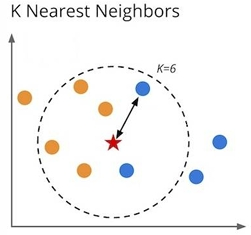
\includegraphics[scale=0.45]{chapter 4/ch4_figure1.jpeg}
\end{wrapfigure}
Here are the steps to implement the K-Nearest Neighbours (KNN) Classifier:\\
\vspace{2mm}
\begin{enumerate}
    \item Prepare Training Data and Test Data.
    \item Select the value of \(K\) (\hl{Number of Neighbours}).
    \item Determine which distance function to use (Euclidean, Manhattan, Cosine, Hamming, etc.).
    \item Compute the distance between the new data point and all the training data points \(n\).
    \item Sort the distances and take the \(K\)-nearest data points.
    \item Assign the new data point to the majority class of the \(K\)-Nearest Neighbours.
\end{enumerate}
\vspace{2mm}
\underline{\textbf{Example of KNN}}\\
Suppose we have the height, weight and T-shirt size of some customers as follows:
\begin{center}
    \begin{tabular}{|m{2.5cm}|m{0.5cm}|m{0.5cm}|m{0.5cm}|m{0.5cm}|m{0.5cm}|m{0.5cm}|m{0.5cm}|m{0.5cm}|m{0.5cm}|m{0.5cm}|m{0.5cm}|m{0.5cm}|m{0.5cm}|m{0.5cm}|m{0.5cm}|m{0.5cm}|m{0.5cm}|m{0.5cm}|}
        \hline
        \cellcolor{lightblue}{\textbf{Height (in cm)}} & 158 & 158 & 158 & 160 & 160 & 163 & 163 & 160 & 163 & 165 & 165 & 165 & 168 & 168 & 168 & 170 & 170 & 170 \\
        \hline
        \cellcolor{lightblue}{\textbf{Weight (in kg)}} & 58 & 59 & 63 & 59 & 60 & 60 & 61 & 64 & 64 & 61 & 62 & 65 & 62 & 63 & 66 & 63 & 64 & 68 \\
        \hline
        \cellcolor{lightblue}{\textbf{T-shirt Size}} & M & M & M & M & M & M & M & L & L & L & L & L & L & L & L & L & L & L \\
        \hline
        \end{tabular}
\end{center}
To predict the T-shirt size of a new customer given only the height and weight, we can use the KNN Classifier.\\
\vspace{3mm}
\uwave{Step 1: Prepare Training Data and Test Data.}\\
Training Data:\\
\begin{center}
    \begin{tabular}{|m{2.5cm}|m{0.5cm}|m{0.5cm}|m{0.5cm}|m{0.5cm}|m{0.5cm}|m{0.5cm}|m{0.5cm}|m{0.5cm}|m{0.5cm}|m{0.5cm}|m{0.5cm}|m{0.5cm}|m{0.5cm}|m{0.5cm}|m{0.5cm}|m{0.5cm}|m{0.5cm}|m{0.5cm}|}
        \hline
        \cellcolor{lightblue}{\textbf{Height (in cm)}} & 158 & 158 & 158 & 160 & 160 & 163 & 163 & 160 & 163 & 165 & 165 & 165 & 168 & 168 & 168 & 170 & 170 & 170 \\
        \hline
        \cellcolor{lightblue}{\textbf{Weight (in kg)}} & 58 & 59 & 63 & 59 & 60 & 60 & 61 & 64 & 64 & 61 & 62 & 65 & 62 & 63 & 66 & 63 & 64 & 68 \\
        \hline
        \cellcolor{lightblue}{\textbf{T-shirt Size}} & M & M & M & M & M & M & M & L & L & L & L & L & L & L & L & L & L & L \\
        \hline
        \end{tabular}
\end{center}
Testing Data: Height = 161 cm, Weight = 61 kg.\\
\vspace{2mm}
\uwave{Step 2: Select the Value of \(K\) (Number of Neighbours).}\\
Let's assume \(K = 5\).\\
\vspace{2mm}
\uwave{Step 3: Determine Which Distance Function to Use.}\\
Let training data with \(n\) attributes be:
\[
    x^{Train} = (x_1^{Train}, x_2^{Train}, \ldots, x_n^{Train})
\]
and testing data with \(n\) attributes be:
\[
    x^{Test} = (x_1^{Test}, x_2^{Test}, \ldots, x_n^{Test})
\]
Assume the Euclidean Distance Formula is used:
\[
    distance(x^{Train}, x^{Test}) = \sqrt{\sum_{i=1}^{n} (x_i^{Train} - x_i^{Test})^2}
\]
\newpage
\uwave{Step 4: Compute the Distance Between the New Data Point to Its \(n\) Training Data Points.}\\
Compute the distance of the new Data with height = 161 cm and weight = 61 kg to all the training data points.\\
\begin{center}
    \begin{tabular}{|m{3cm}|m{0.5cm}|m{0.5cm}|m{0.5cm}|m{0.5cm}|m{0.5cm}|m{0.5cm}|m{0.5cm}|m{0.5cm}|m{0.5cm}|m{0.5cm}|m{0.5cm}|m{0.5cm}|m{0.5cm}|m{0.5cm}|m{0.5cm}|m{0.5cm}|m{0.5cm}|m{0.7cm}|}
        \hline
        \textbf{Height (in cm)} & 158 & 158 & 158 & 160 & 160 & 163 & 163 & 160 & 163 & 165 & 165 & 165 & 168 & 168 & 168 & 170 & 170 & 170 \\
        \hline
        \textbf{Weight (in kg)} & 58 & 59 & 63 & 59 & 60 & 60 & 61 & 64 & 64 & 61 & 62 & 65 & 62 & 63 & 66 & 63 & 64 & 68 \\
        \hline
        \textbf{T-shirt Size} & M & M & M & M & M & M & M & L & L & L & L & L & L & L & L & L & L & L \\
        \hline
        \textbf{Distance between} & & & & & & & & & & & & & & & & & & \\
        \textbf{the training data} & \scriptsize{4.24} & \scriptsize{3.61} & \scriptsize{3.61} & \scriptsize{2.24} & \scriptsize{1.41} & \scriptsize{2.24} & \scriptsize{2.00} & \scriptsize{3.16} & \scriptsize{3.61} & \scriptsize{4.00} & \scriptsize{4.12} & \scriptsize{5.66} & \scriptsize{7.07} & \scriptsize{7.28} & \scriptsize{8.60} & \scriptsize{9.22} & \scriptsize{9.49} & \scriptsize{11.40} \\
        \textbf{and testing data} & & & & & & & & & & & & & & & & & & \\
        \hline
        \end{tabular}
\end{center}
\uwave{Step 5: Sort the Distances Obtained and Take the \(K\)-Nearest Data Points.}\\
Sort the distances in ascending order and take the \(K = 5\)-nearest data points.\\
\begin{center}
    \begin{tabular}{|m{3cm}|m{0.5cm}|m{0.5cm}|m{0.5cm}|m{0.5cm}|m{0.5cm}|m{0.5cm}|m{0.5cm}|m{0.5cm}|m{0.5cm}|m{0.5cm}|m{0.5cm}|m{0.5cm}|m{0.5cm}|m{0.5cm}|m{0.5cm}|m{0.5cm}|m{0.5cm}|m{0.7cm}|}
        \hline
        \textbf{Height (in cm)} & \textcolor{red}{160} & \textcolor{red}{163} & \textcolor{red}{160} & \textcolor{red}{163} & \textcolor{red}{160} & 158 & 158 & 163 & 165 & 165 & 158 & 165 & 168 & 168 & 168 & 170 & 170 & 170 \\
        \hline
        \textbf{Weight (in kg)} & \textcolor{red}{60} & \textcolor{red}{61} & \textcolor{red}{59} & \textcolor{red}{60} & \textcolor{red}{64} & 59 & 63 & 64 & 61 & 62 & 58 & 65 & 62 & 63 & 66 & 63 & 64 & 68 \\
        \hline
        \textbf{T-shirt Size} & \textcolor{red}{M} & \textcolor{red}{M} & \textcolor{red}{M} & \textcolor{red}{M} & \textcolor{red}{L} & M & M & L & L & L & M & L & L & L & L & L & L & L \\
        \hline
        \textbf{Distance between} & & & & & & & & & & & & & & & & & & \\
        \textbf{the training data} & \textcolor{red}{\scriptsize{1.41}} & \textcolor{red}{\scriptsize{2.00}} & \textcolor{red}{\scriptsize{2.24}} & \textcolor{red}{\scriptsize{2.24}} & \textcolor{red}{\scriptsize{3.16}} & \scriptsize{3.61} & \scriptsize{3.61} & \scriptsize{3.61} & \scriptsize{4.00} & \scriptsize{4.12} & \scriptsize{4.24} & \scriptsize{5.66} & \scriptsize{7.07} & \scriptsize{7.28} & \scriptsize{8.60} & \scriptsize{9.22} & \scriptsize{9.49} & \scriptsize{11.40} \\
        \textbf{and testing data} & & & & & & & & & & & & & & & & & & \\
        \hline
        \end{tabular}
\end{center}
\uwave{Step 6: Assign the New Data Point Based on the Majority Class of the \(K\)-Nearest Neighbours.}\\
\begin{center}
    \begin{tabular}{|m{3cm}|m{0.6cm}|m{0.6cm}|m{0.6cm}|m{0.6cm}|m{0.6cm}|}
        \hline
        \textbf{Height (in cm)} & 160 & 163 & 160 & 163 & 160 \\
        \hline
        \textbf{Weight (in kg)} & 60 & 61 & 59 & 60 & 64 \\
        \hline
        \textbf{T-shirt Size} & M & M & M & M & L \\
        \hline
        \textbf{Distance between} & & & & & \\
        \textbf{the training data} & 1.41 & 2.00 & 2.24 & 2.24 & 3.16 \\
        \textbf{and testing data} & & & & & \\
        \hline
        \end{tabular}
\end{center}
Among the 5-nearest customers, 4 of them had "Medium T-shirt Sizes" and 1 had a "Large T-shirt Size", which classifies the test data to "Medium T-shirt Size".\\
\textcolor{red}{$\therefore$ The best guess for the customer with height = 161 cm and weight = 61 kg is a \uuline{"Medium T-shirt Size"}}.\\
\vspace{4mm}
\textit{\large{KNN Classifier Python Code Implementation using Scikit-Learn:}}
\begin{lstlisting}[language=Python, basicstyle=\ttfamily\small, keywordstyle=\color{blue}, commentstyle=\color{forestgreen}, stringstyle=\color{red}]
from sklearn.preprocessing import LabelEncoder      # Import LabelEncoder functions
from sklearn.Neighbors import KNeighborsClassifier  # Import KNN Classifier functions
import numpy as np                                  # Import numpy functions

# Assign features and label variables
# Features: Height, Weight
height = np.array([158, 158, 158, 160, 160, 163, 163, 160, 163, 165,
                   165, 165, 168, 168, 168, 170, 170, 170])
weight = np.array([58, 59, 63, 59, 60, 60, 61, 64, 64, 61, 62, 65, 62, 63, 66, 63, 64, 68])
size = np.array(['M', 'M', 'M', 'M', 'M', 'M', 'M', 'L', 'L', 'L', 
                 'L', 'L', 'L', 'L', 'L', 'L', 'L', 'L'])

# Create LabelEncoder that used to convert string labels into numbers
encoder = LabelEncoder()
# Convert the string labels into numbers
label = encoder.fit_transform(size)
# Combine height and weight into a single list of tuples
features = list(zip(height, weight))

# Create KNN Classifier and set K = 5
model = KNeighborsClassifier(n_neighbors=5)
# Train the model using the training sets
model.fit(features, label)

# Predict the class for the new data point
predicted = model.predict([[161, 61]])              # Height = 161 cm, Weight = 61 kg

# Convert the predicted class into string
result = encoder.inverse_transform(predicted)
# Print the result
print(result)

# Output: ['M']
\end{lstlisting}
\newpage
\textcolor{magenta}{\section{\textbf{Standardization in KNN Classifier}}}
\subsection{Defintion and Practice of Standardization in KNN Classifier}
When the training data are \textcolor{violet}{measured in different units}, it is important to \textcolor{violet}{standardize the data} before applying the KNN Classifier.\\
\begin{thmBox}{Theorem 4.3}{Standardization in KNN Classifier}
    \textcolor{cyan}{Standardization} is the process of \textcolor{cyan}{rescaling the features} to make the attributes \textcolor{cyan}{comparable} to each other.\\
    The formula for standardization is:
    \[
        X_{new} = \frac{X - \mu}{\sigma}
    \]
    where:
    \begin{description}
        \item[\textcolor{brown}{\(X\)}]: Attribute Value
        \item[\textcolor{brown}{\(X_{new}\)}]: Standardized Attribute Value
        \item[\textcolor{brown}{\(\mu\)}]: Mean of the Attribute Value of all training data
        \item[\textcolor{brown}{\(\sigma\)}]: Standard Deviation of the Attribute Value of all training data
    \end{description}
\end{thmBox}
\vspace{2mm}
\underline{\textbf{Example of Standardization in KNN Classifier}}\\
\vspace{1mm}
\begin{center}
    \begin{tabular}{|m{3cm}|m{0.5cm}|m{0.5cm}|m{0.5cm}|m{0.5cm}|m{0.5cm}|m{0.5cm}|m{0.5cm}|m{0.5cm}|m{0.5cm}|m{0.5cm}|m{0.5cm}|m{0.5cm}|m{0.5cm}|m{0.5cm}|m{0.5cm}|m{0.5cm}|m{0.5cm}|m{0.7cm}|}
        \hline
        \textbf{Height (in cm)} & \textcolor{red}{160} & \textcolor{red}{163} & \textcolor{red}{160} & \textcolor{red}{163} & 160 & 158 & 158 & 163 & \textcolor{red}{165} & 165 & 158 & 165 & 168 & 168 & 168 & 170 & 170 & 170 \\
        \hline
        \textbf{Weight (in kg)} & \textcolor{red}{60} & \textcolor{red}{61} & \textcolor{red}{59} & \textcolor{red}{60} & 64 & 59 & 63 & 64 & \textcolor{red}{61} & 62 & 58 & 65 & 62 & 63 & 66 & 63 & 64 & 68 \\
        \hline
        \textbf{T-shirt Size} & \textcolor{red}{M} & \textcolor{red}{M} & \textcolor{red}{M} & \textcolor{red}{M} & L & M & M & L & \textcolor{red}{L} & L & M & L & L & L & L & L & L & L \\
        \hline
        \textbf{Distance between} & & & & & & & & & & & & & & & & & & \\
        \textbf{the training data} & \textcolor{red}{\scriptsize{1.41}} & \textcolor{red}{\scriptsize{2.00}} & \textcolor{red}{\scriptsize{2.24}} & \textcolor{red}{\scriptsize{2.24}} & \scriptsize{3.16} & \scriptsize{3.61} & \scriptsize{3.61} & \scriptsize{3.61} & \textcolor{red}{\scriptsize{4.00}} & \scriptsize{4.12} & \scriptsize{4.24} & \scriptsize{5.66} & \scriptsize{7.07} & \scriptsize{7.28} & \scriptsize{8.60} & \scriptsize{9.22} & \scriptsize{9.49} & \scriptsize{11.40} \\
        \textbf{and testing data} & & & & & & & & & & & & & & & & & & \\
        \hline
        \textbf{Distance between} & & & & & & & & & & & & & & & & & & \\
        \textbf{the training data} & & & & & & & & & & & & & & & & & & \\
        \textbf{and testing data} & \textcolor{orange}{\scriptsize{0.44}} & \textcolor{orange}{\scriptsize{0.46}} & \textcolor{orange}{\scriptsize{0.60}} & \textcolor{orange}{\scriptsize{0.79}} & \scriptsize{1.16} & \scriptsize{1.03} & \scriptsize{1.03} & \scriptsize{1.23} & \textcolor{orange}{\scriptsize{0.92}} & \scriptsize{1.00} & \scriptsize{1.33} & \scriptsize{1.78} & \scriptsize{1.66} & \scriptsize{1.79} & \scriptsize{2.49} & \scriptsize{2.22} & \scriptsize{2.37} & \scriptsize{3.37} \\
        \textbf{(Standardization)} & & & & & & & & & & & & & & & & & & \\
        \hline
        \end{tabular}
\end{center}
Mean of Height = \uuline{164 cm}, Standard Deviation of Height = \uuline{4.33 cm}\\
Mean of Weight = \uuline{62.33 kg}, Standard Deviation of Weight = \uuline{2.63 kg}\\
\vspace{1mm}
After standardization using the formula \(X_{new} = \frac{X - \mu}{\sigma}\) with the testing data point (Height = 161 cm, Weight = 61 kg), we have:\\
\[
    \textcolor{orange}{\text{Standardized Height}} = \frac{161 - 164}{4.33} = \underline{\underline{-0.69}}
\]
\[
\textcolor{orange}{\text{Standardized Weight}} = \frac{61 - 62.33}{2.63} = \underline{\underline{-0.51}}
\]\\
\vspace{1mm}
The 5th closest value got changed as height was dominating earlier, but after standardization, weight is also considered.\\
\vspace{2mm}
\newpage
\textit{\large{Standardization in KNN Classifier Python Code Implementation using Scikit-Learn:}}

\begin{lstlisting}[language=Python, basicstyle=\ttfamily\small, keywordstyle=\color{blue}, commentstyle=\color{forestgreen}, stringstyle=\color{red}]
from sklearn.preprocessing import StandardScaler    # Import StandardScaler functions
from sklearn.neighbors import KNeighborsClassifier  # Import KNN Classifier functions
import numpy as np                                  # Import numpy functions

# Assign features and label variables
# Feature: Height
height = np.array([158, 158, 158, 160, 160, 163, 163, 160, 163, 165,
                   165, 165, 168, 168, 168, 170, 170, 170])
h_means = np.mean(height)           # Mean of Height
h_std = np.std(height, ddof=1)      # Standard Deviation of Height, ddof=1 is to make the divisor N-1
height = (height - h_means) / h_std # Standardize Height

# Feature: Weight
weight = np.array([58, 59, 63, 59, 60, 60, 61, 64, 64, 61, 62, 65, 62, 63, 66, 63, 64, 68])
w_means = np.mean(weight)           # Mean of Weight
w_std = np.std(weight, ddof=1)      # Standard Deviation of Weight, ddof=1 is to make the divisor N-1
weight = (weight - w_means) / w_std # Standardize Weight

size = np.array(['M', 'M', 'M', 'M', 'M', 'M', 'M', 'L', 'L', 'L', 
                 'L', 'L', 'L', 'L', 'L', 'L', 'L', 'L'])

# Create LabelEncoder that used to convert string labels into numbers
encoder = LabelEncoder()
# Convert the string labels into numbers
label = encoder.fit_transform(size)
# Combine height and weight into a single list of tuples
features = list(zip(height, weight))

# Create KNN Classifier and set K = 5
model = KNeighborsClassifier(n_neighbors=5)
# Train the model using the training sets
model.fit(features, label)

# Standardize the new data point
new_height = (161 - h_means) / h_std
new_weight = (61 - w_means) / w_std
# Predict the Output for the new data point
predicted = model.predict([[new_height, new_weight]])
# Convert the predicted class into string
result = encoder.inverse_transform(predicted)
# Print the result
print(result)

# Output: ['M']
\end{lstlisting}
\newpage
\subsection{Standard Deviation}
\textcolor{cyan}{Standard Deviation} is one of the \textcolor{violet}{most common ways to measure the spread of values in a dataset}.\\
There are \textcolor{violet}{two types of Standard Deviation}:
\begin{description}
    \item[$\bullet$] \textcolor{cyan}{\textbf{Population Standard Deviation}}
    \item[$\bullet$] \textcolor{cyan}{\textbf{Sample Standard Deviation}}
\end{description}
\textcolor{olive}{\subsubsection{Population Standard Deviation}}
We calculate the \textcolor{violet}{Population Standard Deviation} when the dataset we are working with \textcolor{violet}{represents the entire population (Every value that we are interested in)}.\\
\begin{thmBox}{Theorem 4.3.2.1}{Population Standard Deviation}
    The formula for calculating the \textcolor{cyan}{Population Standard Deviation} is:
    \[
        \sigma = \sqrt{\frac{\sum_{i=1}^{N} (X_i - \mu)^2}{N}}
    \]
    where:
    \begin{description}
        \item[\textcolor{brown}{\(X_i\)}]: i-th Value in the Dataset
        \item[\textcolor{brown}{\(\mu\)}]: Mean of the Population
        \item[\textcolor{brown}{\(N\)}]: Size of the Population
    \end{description}
\end{thmBox}
\textcolor{olive}{\subsubsection{Sample Standard Deviation}}
We calculate the \textcolor{violet}{Sample Standard Deviation} when the dataset we are working with \textcolor{violet}{represents a sample taken from a large population of interest}.\\
\begin{thmBox}{Theorem 4.3.2.2}{Sample Standard Deviation}
    The formula for calculating the \textcolor{cyan}{Sample Standard Deviation} is:
    \[
        s = \sqrt{\frac{\sum_{i=1}^{N} (X_i - \bar{X})^2}{N-1}}
    \]
    where:
    \begin{description}
        \item[\textcolor{brown}{\(X_i\)}]: i-th Value in the Dataset
        \item[\textcolor{brown}{\(\bar{X}\)}]: Mean of the Sample
        \item[\textcolor{brown}{\(N\)}]: Size of the Sample
    \end{description}
\end{thmBox}
\textcolor{olive}{\subsubsection{Difference between Population and Sample Standard Deviation}}
Difference: When calculating the \textcolor{violet}{Population Standard Deviation}, we divide by the \textcolor{violet}{size of the population}, while for the \textcolor{violet}{Sample Standard Deviation}, we divide by the \textcolor{violet}{size of the sample minus 1}.\\
When we caclculate the \textcolor{violet}{Sample Standard Deviation}, we tend to \textcolor{violet}{underestimate the true variability of the population }(Our estimate of true population standard is biased).\\
To \textcolor{violet}{correct this bias}, we divide by \(N-1\) instead of \(N\) in the denominator to make the sample standard deviation an \textcolor{violet}{unbiased estimator of the population standard deviation}.\\
\newpage
\textcolor{magenta}{\section{\textbf{Distance Functions/Metrics in KNN Classifier}}}

\subsection{Introduction to Distance Functions in KNN Classifier}
\begin{wrapfigure}[1]{r}{0.4\textwidth}
    \centering
    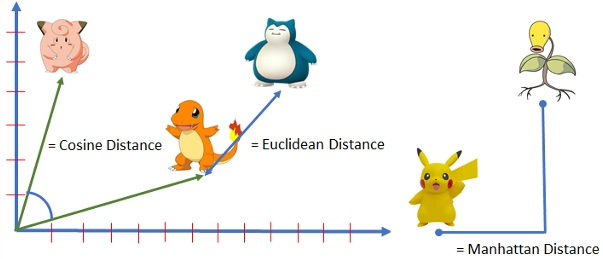
\includegraphics[scale=0.35]{chapter 4/ch4_figure2.jpeg}
    \caption{Distance Functions in KNN}
\end{wrapfigure}

\textcolor{cyan}{Distance Functions} are used to \textcolor{cyan}{measure the similarity between two data points} in the KNN Classifier.\\
There are \textcolor{violet}{several distance functions} that are available in the KNN Classifier, such as:
\begin{description}
    \item[$\bullet$] \textcolor{cyan}{\textbf{Euclidean Distance}}
    \item[$\bullet$] \textcolor{cyan}{\textbf{Manhattan Distance (City Block Distance)}}
    \item[$\bullet$] \textcolor{cyan}{\textbf{Cosine Distance}}
    \item[$\bullet$] \textcolor{cyan}{\textbf{Hamming Distance}}
\end{description}
\vspace{4mm}
\subsection{Euclidean Distance}
\begin{thmBox}{Theorem 4.4.1}{Euclidean Distance}
    \textcolor{cyan}{Euclidean Distance} is the \textcolor{cyan}{straight-line distance} between two points in Euclidean space.\\
    The formula for calculating the \textcolor{cyan}{Euclidean Distance} between \(n\) data points is:
    \[
        \text{Euclidean Distance} = \sqrt{\sum_{i=1}^{n} (x_i^{Train} - x_i^{Test})^2}
    \]
\end{thmBox}
\begin{egBox}{Example 4.4.1}{Euclidean Distance}
    Suppose we have Training Data: (Height, Weight) = (160 cm, 60 kg) and Testing Data: (Height, Weight) = (163 cm, 61 kg).\\
    The Euclidean Distance between the two points is:
    \[
        \sqrt{(160 - 163)^2 + (60 - 61)^2} = \sqrt{(-3)^2 + (-1)^2} = \sqrt{9 + 1} = \sqrt{10} \approx 3.16
    \]
\end{egBox}
\vspace{4mm}
\subsection{Manhattan Distance}
\begin{thmBox}{Theorem 4.4.2}{Manhattan Distance}
    \textcolor{cyan}{Manhattan Distance} is the \textcolor{cyan}{sum of the absolute differences} between the \(x\) and \(y\) coordinates of two points.\\
    The formula for calculating the \textcolor{cyan}{Manhattan Distance} between \(n\) data points is:
    \[
        \text{Manhattan Distance} = \sum_{i=1}^{n} |x_i^{Train} - x_i^{Test}|
    \]
\end{thmBox}
\begin{egBox}{Example 4.4.2}{Manhattan Distance}
    Suppose we have Training Data: (Height, Weight) = (160 cm, 60 kg) and Testing Data: (Height, Weight) = (163 cm, 61 kg).\\
    The Manhattan Distance between the two points is:
    \[
        |160 - 163| + |60 - 61| = |-3| + |-1| = 3 + 1 = 4
    \]
\end{egBox}
Manhatten Distance is preferred over Euclidean Distance if \hl{the data set is large} and \hl{less computational power is available}.\\
\newpage
\subsection{Cosine Distance}
\begin{thmBox}{Theorem 4.4.3}{Cosine Distance}
    \textcolor{cyan}{Cosine Distance} is the \textcolor{cyan}{cosine of the angle between two vectors} in an \(n\)-dimensional space.\\
    The formula for calculating the \textcolor{cyan}{Cosine Distance} between \(n\) data points is:
    \[
        \text{Cosine Distance} = 1 - cos(\theta) = 1 - \frac{\sum_{i=1}^{n} (x_i^{Train} \cdot x_i^{Test})}{\sqrt{\sum_{i=1}^{n} (x_i^{Train})^2} \cdot \sqrt{\sum_{i=1}^{n} (x_i^{Test})^2}}
    \]
\end{thmBox}
\begin{egBox}{Example 4.4.3}{Cosine Distance}
    Suppose we have Training Data: (Height, Weight) = (160 cm, 60 kg) and Testing Data: (Height, Weight) = (163 cm, 61 kg).\\
    The Cosine Distance between the two points is:
    \[
        1 - \frac{(160 \cdot 163) + (60 \cdot 61)}{\sqrt{160^2 + 60^2} \cdot \sqrt{163^2 + 61^2}} = 1 - 0.99999977 = 2.26 \times 10^{-7}
    \]
\end{egBox}
Using Cosine Distance, we get \textcolor{violet}{values between 0 and 2}, where:\\
\begin{description}
    \item[$\bullet$] \textcolor{cyan}{0 (Perfect Similarity)}: The training data and test data are \textcolor{violet}{100\% similar to each other}.
    \item[$\bullet$] \textcolor{cyan}{2 (Perfect Dissimilarity)}: The training data and test data are \textcolor{violet}{absolutely different to each other}.
    \item[$\bullet$] \textcolor{cyan}{Values between 0 and 2}: \textcolor{violet}{Varying degrees of similarity}.
\end{description}
\subsection{Hamming Distance}
\begin{thmBox}{Theorem 4.4.4}{Hamming Distance}
    \textcolor{cyan}{Hamming Distance} is the \textcolor{cyan}{number of bit positions in which two bits are different} while comparing two binary strings of equal length.\\
    $\Rightarrow$ A way for comparing two binary data strings, mainly for \hl{categorical data}.\\
    The formula for calculating the \textcolor{cyan}{Hamming Distance} between \(n\) data points is:
    \[
        \text{Hamming Distance} = \sum_{i=1}^{n} (x_i^{Train} \neq x_i^{Test})
    \]
\end{thmBox}
\begin{egBox}{Example 4.4.4}{Hamming Distance}
    Suppose there are two strings 1101 1001 and 1001 1101.\\
    The Hamming Distance between the two strings is:
    \begin{center}
        \begin{tabular}{|c|c|c|c|c|c|c|c|}
            \hline
            1 & 1 & 0 & 1 & 1 & 0 & 0 & 1 \\
            \hline
            1 & 0 & 0 & 1 & 1 & 1 & 0 & 1 \\
            \hline
            \textcolor{forestgreen}{0} & \textcolor{red}{+1} & \textcolor{forestgreen}{0} & \textcolor{forestgreen}{0} & \textcolor{forestgreen}{0} & \textcolor{red}{+1} & \textcolor{forestgreen}{0} & \textcolor{forestgreen}{0} \\
        \end{tabular}
    \end{center}
    The Hamming Distance between the two strings is \textcolor{red}{2}.
\end{egBox}
\textcolor{magenta}{\section{\textbf{K Estimation in KNN Classifier}}}
\subsection{Good Value of K in KNN Classifier}
A \textcolor{cyan}{Low K-value} is \textcolor{violet}{sensitive to outliers} and a \textcolor{cyan}{High K-value} is \textcolor{violet}{more resilient to outliers} as it considers more data points to decide prediction.\\
\textcolor{cyan}{Break the tie} of finding the best value of \(K\) by \hl{Decreasing K by 1} until the tie is broken and \textcolor{violet}{Putting more weight on the closest data points} than the farther ones.\\
The value of \(K\) should \textcolor{violet}{not be too small or too large}, but should be \textcolor{violet}{odd} to avoid ties.\\
There are two methods to find the best value of \(K\): \textcolor{cyan}{\textbf{Rule of Thumb}} and \textcolor{cyan}{\textbf{Cross-Validation}}.
\subsection{Rule of Thumb}
\begin{thmBox}{Theorem 4.5.1}{Rule of Thumb}
    \raggedright
    The \textcolor{cyan}{Rule of Thumb} to find the best value of \(K\) is: \\
    \begin{center}
        Set Heuristic \(K = \sqrt{N}\) \\
    \end{center}
    where \(N\) is the number of training examples in the dataset.
\end{thmBox}
\newpage
\textbf{\large{\textit{Proof:}}}\\
Adapting from Devroye, Gyorfi and Lugosi (1996), the theoretical performance of the KNN Classifier can be organized, albeit not exclusively, in the following way:
\begin{itemize}
    \item \(K\) is determined to be a finite and fixed constantt whilst the sample size \(N \rightarrow \infty\). The determination of \(N\) is a priori after exploratory data analysis or using a heuristic.
    \item \(K \rightarrow \infty\) whilst \(\frac{K}{N} \rightarrow 0\), but now \(K\) is not fixed relative to \(N\).
    \item Data dependent methods for determining \(K\) are used, such as using a training set and selecting the value of \(K\) that minimizes the estimated classification error rate / using cross-validation.
\end{itemize}
The heuristic \(K = \floor{\sqrt{N}}\) where \(\floor{\sqrt{N}}\) is the floor of the square root of \(N\), would fall under the second category.\\
The following is a quantitative, fintie-sample probabilistic bound on the excess risk \(L_n - L^*\) of the KNN Classifier, whihc in turn implies an asymptotic result: \\
\fbox{
    \parbox{0.97\textwidth}{
        Assume that each \(\mu\) has a density. If \(K \rightarrow \infty\) and \(\frac{K}{N} \rightarrow 0\), then for every \(\epsilon > 0\), there is an \(N_0\) such that for all \(N > N_0\):
        \[
            P\left(L_n - L^* > \epsilon\right) \leq 2e^{\frac{-N\epsilon^2}{72\gamma_d^{2}}}
        \]
        where the constant \(\gamma_d\) is defined as the minimal number of cones centered at the origin of angle \(\frac{\pi}{6}\) that covers \(\mathbb{R}^d\).\\
        $\therefore$ The KNN Rule is strongly consistent.
    }
}

\vspace{1mm}
Supplying the context on the terms not defined in the extract: \(L_N = L_N(g_N) = P(g_N(X) \neq Y)\) is the risk of the KNN Classifier \(g_N\) where \(g_N\) is estimated from the sample size \(N\).\\
The Bayes-optimal risk/Bayes error rate \(L^* = L(g^x) = inf_{g\in G} P(g(X) \neq Y)\) is the risk of the Bayes-optimal classifier \(g^*\). Glossing over the measure theoretic technicalities measuring \(\mu\) has a density means that X has a density.\\
Parsing the theorem, the main condition requires that \(K \rightarrow \infty\) as the sample size \(N \rightarrow \infty\) so that \(\frac{K}{N} \rightarrow 0\). Our heuristic satisfies this condition since \(K = \floor{\sqrt{N}} \rightarrow \infty \) and \(\frac{K}{N} = \frac{\floor{\sqrt{N}}}{N} = \frac{\sqrt{N}}{N} = \frac{1}{\sqrt{N}} \rightarrow 0\) as \(N \rightarrow \infty\).\\
\vspace{1mm}
Taking the theorem as an asymptotic result, the KNN classifier is strongly consistent:
\[
    L_N \xrightarrow{a.s.} L^* \Longleftrightarrow P\left(\lim_{N \rightarrow \infty} L_N = L^*\right) = 1
\]
As we collect more observations \(N \rightarrow \infty\), the classification error rate \(L_N\) of the KNN classifier \(g_N\) will coverge surely to the minimal classification error rate \(L^*\) we can possibly hope to achieve, which converges exponentially quickly to 0.\\
The result is non-asymptotic in that for finite \(N\). It bounds the probability that \(L_N\) deviates from \(L^*\) by more than \(\epsilon\) for any \(\epsilon > 0\).\\
\textbf{On the Use of Data-Dependent Methods for Selecting K}:\\
The utility of the above theoretical result then is that it supplies insight on heuristics like the one we have outlined.\\
Its limitations are that the constant \(\gamma_d\) may be difficult to compute, which renders the bound too loose to give any practical prescriptions.\\
Echoing the sentiment expressed:
\fbox{
    \parbox{0.97\textwidth}{
        KNN density linkage is strongly set consistent for high-density/density-contour clusters if K is chosen that \(\frac{K}{N} \rightarrow 0\) and \(\frac{K}{ln(N)} \rightarrow \infty\) as \(N \rightarrow \infty\).
    }
}

\vspace{1mm}
Data-dependent means of selecting K in practice is used:
\fbox{
    \parbox{0.97\textwidth}{
        Consistency by itself may be obtained by choosing \(K = \floor{\sqrt{N}}\), but few if any users will want to blindly use such recipes.\\
        Instead, a healthy dose of feedback from the data is preferable.
    }
}

\vspace{1mm}
Similar consistency results for the use of a test set to select K based on minimising a holdout estimate of the classification error rate are supplied therein.\\

\subsection{Cross-Validation}
\begin{wrapfigure}[2]{r}{0.35\textwidth}
    \centering
    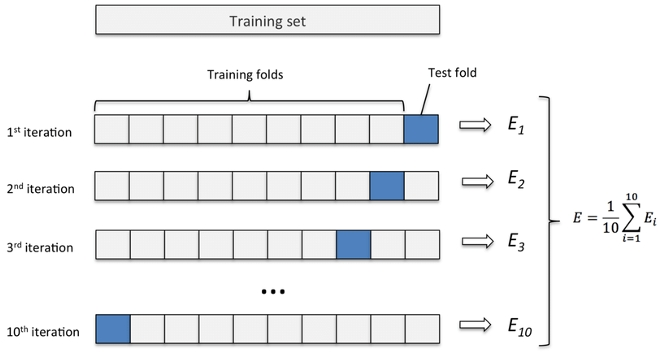
\includegraphics[scale=0.3]{chapter 4/ch4_figure3.jpeg}
    \caption{Cross-Validation in KNN}
\end{wrapfigure}
Suppose we select K using \textcolor{cyan}{d-fold Cross-Validation}.\\
Steps to perform Cross-Validation:
\begin{enumerate}
    \item Split the training data into \textcolor{violet}{\(d\) groups/folds of approximately equal size}. 
    \item \textcolor{cyan}{Validation Set}: Hold the \textcolor{violet}{first group}.
    \item \textcolor{cyan}{Train} our KNN classifier on the \textcolor{violet}{remaining \(d-1\) groups of data}.
    \item For each value of \(K\):
        \begin{itemize}
            \item \textcolor{cyan}{Classify each data in the validation set} using the KNN classifier in the training set.
            \item \textcolor{cyan}{Record the error}.
        \end{itemize}
    \item \textcolor{cyan}{Repeat the above steps 1-4 for all \(d\) groups} of the validation.
    \item For \textcolor{violet}{each choice of \(K\)}, \textcolor{cyan}{Average the error across validation sets}. \\
    \textcolor{cyan}{Choose the value of K with the lowest error}
\end{enumerate}
\newpage
\textcolor{magenta}{\section{\textbf{Error Measurements in KNN Classifier}}}
\subsection{Error Measurement for Regression Problems}
There are many ways to \textcolor{violet}{measure errors}. For example:
\begin{itemize}
    \item \textcolor{cyan}{Mean Absolute Error (MAE)}
    \[
        \text{MAE} = \frac{\sum_{i=1}^{m} |a_i - p_i|}{m}
    \]
    \item \textcolor{cyan}{Mean Squared Error (MSE)}
    \[
        \text{MSE} = \frac{\sum_{i=1}^{m} (a_i - p_i)^2}{m}
    \]
    \item \textcolor{cyan}{Mean Absolute Percentage Error (MAPE)}
    \[
        \text{MAPE} = \frac{\sum_{i=1}^{m} \left|\frac{a_i - p_i}{a_i}\right|}{m} \times 100\%
    \]
\end{itemize}
where \(a_i\) is the actual labels and \(p_i\) is the predicted labels.
\subsection{Error Measurement for Classification Problems}
When dealing with \textcolor{violet}{Classification Problems}, the error can be calculated using \(1 - \text{F1-Score}\), where F1-score is determined by \textcolor{cyan}{True Positive (TP)}, \textcolor{cyan}{False Positive (FP)}, \textcolor{cyan}{True Negative (TN)} and \textcolor{cyan}{False Negative (FN)} for each class. \\
These values are obtained from the \textcolor{cyan}{Confusion Matrix}, which is one of the Model Evaluation Techniques.\\
\vspace{1mm}
Lists of Model Evaluation Techniques:
\begin{itemize}
    \item Confusion Matrix
    \item Precision, Recall and F1-Score
    \item Matthews Correlation Coefficient (MCC)
\end{itemize}
\textcolor{olive}{\subsubsection{2x2 Confusion Matrix}}

\begin{wrapfigure}[1]{r}{0.17\textwidth}
    \centering
    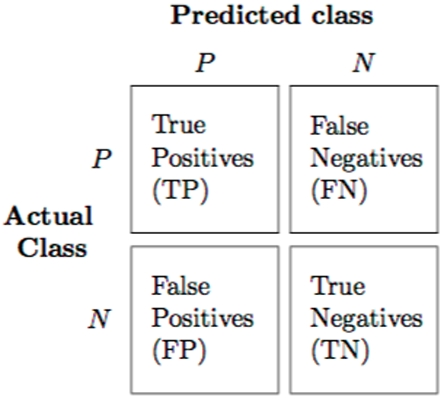
\includegraphics[scale=0.2]{chapter 4/ch4_figure4.jpeg}
\end{wrapfigure}
There are 4 important values in the 2x2 Confusion Matrix:\\
\begin{itemize}
    \item \textcolor{cyan}{True Positive (TP)}: Number of predictions where the classifier \textcolor{violet}{correctly predicts the positive class as positive}.
    \item \textcolor{cyan}{True Negative (TN)}: Number of predictions where the classifier \textcolor{violet}{correctly predicts the negative class as negative}.
    \item \textcolor{cyan}{False Positive (FP)}: Number of predictions where the classifier \textcolor{violet}{incorrectly predicts the negative class as positive}.
    \item \textcolor{cyan}{False Negative (FN)}: Number of predictions where the classifier \textcolor{violet}{incorrectly predicts the positive class as negative}.
\end{itemize}
\(Error = \frac{FP + FN}{TP + TN + FP + FN}\)\\
\vspace{1mm}
\(Accuracy = \frac{TP + TN}{TP + TN + FP + FN}\)\\
\textcolor{olive}{\subsubsection{Precision, Recall and F1-Score}}
\textcolor{cyan}{\textbf{Precision}}: What fraction of predicts as a \textcolor{violet}{positive class is actually positive}?
\[
    \text{Precision} = \frac{TP}{TP + FP}
\]
\textcolor{cyan}{\textbf{Recall}}: What fraction of the \textcolor{violet}{positive samples are correctly predicted as positive} by the classifier?
\[
    \text{Recall} = \frac{TP}{TP + FN}
\]
\textcolor{cyan}{\textbf{F1-Score}}: The \textcolor{violet}{harmonic mean of Precision and Recall}.
\[
    \text{F1-Score} = 2 \times \frac{\text{Precision} \times \text{Recall}}{\text{Precision} + \text{Recall}} = \frac{2TP}{2TP + FP + FN}
\]
In perfect world, the precision and recall are 1, meaning F1-Score is 1. However, a 100\% accuracy is not the case for machine learning models.\\
\newpage
\textcolor{olive}{\subsubsection{Matthews Correlation Coefficient (MCC)}}
\textcolor{cyan}{Matthew's Correlation Coefficient Formula (MCC)} is the \textcolor{violet}{best single-value classification metric} which helps to \textcolor{violet}{summarize the confusion matrix/error matrix}.\\
\[
    \text{MCC} = \frac{TN \times TP - FN \times FP}{\sqrt{(TP + FP)(TP + FN)(TN + FP)(TN + FN)}}
\]
If the prediction returns good rates for all 4 of these values (TP, TN, FP, FN), then the MCC value will have a reliable measure producing high scores.\\
To suit the most correlation, MCC ranges \textcolor{red}{from -1 to +1}.\\
\begin{itemize}
    \item \textcolor{cyan}{+1}: Best agreement between prediction and actual data.
    \item \textcolor{cyan}{0}: No agreement between prediction and actual data, meaning random prediction.
    \item \textcolor{cyan}{-1}: Worst agreement between prediction and actual data.
\end{itemize}
\begin{egBox}{Example 4.6.2.3}{}
    Suppose we have a 2x2 Conufusion Matrix with entries: \(TP = 90\), \(FP = 4\), \(TN = 1\), \(FN = 5\).\\
    When we substitute these values into the MCC formula, we get:
    \[
        \text{MCC} = \frac{1 \times 90 - 5 \times 4}{\sqrt{(90 + 4)(90 + 5)(1 + 4)(1 + 5)}} = \frac{90 - 20}{\sqrt{94 \times 95 \times 5 \times 6}} = \frac{70}{\sqrt{267900}} \approx 0.13524203\ldots
    \]
    \(0.13524203\ldots\) of the MCC means the classifier is very close to a random guess classifier.\\
    $\therefore$ The MCC helps us to identify the ineffectiveness of the classifier in classifying especially the negative class samples.
\end{egBox}
\textcolor{olive}{\subsubsection{Confusion Matrix for Multi-Class}}

\begin{wrapfigure}[2]{r}{0.35\textwidth}
    \centering
    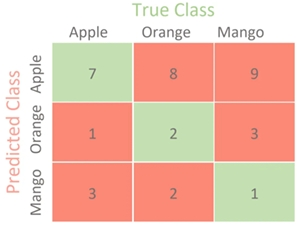
\includegraphics[scale=0.55]{chapter 4/ch4_figure5.jpeg}
\end{wrapfigure}

Unlike binary classification, there are no positive or negative class.\\
Take Apple as example to find TP, TN, FP and FN:\\
\begin{itemize}
    \item TP: Both actual and predicted values are apples, \(TP = 7\).
    \item TN: Both actual and predicted values are non-apples, \(TN = 1+2+2+3=8\).
    \item FP: Predicted value is apple, but actual value is non-apple, \(FP = 8+9=17\).
    \item FN: Predicted value is non-apple, but actual value is apple, \(FN = 1+3=4\).
\end{itemize}
\(\text{Precision} = \frac{TP}{TP + FP} = \frac{7}{7+17} = \frac{7}{24} = 0.2917\)\\
\vspace{1mm}
\(\text{Recall} = \frac{TP}{TP + FN} = \frac{7}{7+4} = \frac{7}{11} = 0.6364\)\\
\vspace{1mm}
\(\text{F1-Score} = \frac{2 \times TP}{2 \times TP + FP + FN} = \frac{2 \times 7}{2 \times 7 + 17 + 4} = \frac{14}{35} = 0.4\)\\
\vspace{1mm}
\(\text{Error} = 1 - \text{F1-Score} = 1 - 0.4 = 0.6\)\\
We can calculate the measures for the other classes (Orange, Manago).
\begin{center}
    \begin{tabular}{|c|c|c|c|}
        \hline
        \rowcolor{lightblue}
        \textbf{Class} & \textbf{Precision} & \textbf{Recall} & \textbf{F1-Score} \\
        \hline
        Apple & 0.29 & 0.64 & 0.40 \\
        \hline
        Orange & 0.33 & 0.17 & 0.22 \\
        \hline
        Manago & 0.17 & 0.08 & 0.11 \\
        \hline
    \end{tabular}
\end{center}
To combine the F1-score of each class to have a single measure for the whole Confusion Matrix Model, we can use the \textcolor{cyan}{\textbf{Macro F1}}, \textcolor{cyan}{\textbf{Micro F1}} or \textcolor{cyan}{\textbf{Weighted F1}}.
\textcolor{teal}{\paragraph{Micro F1}}
\textcolor{cyan}{Micro-Averaged F1-Score (Micro F1)} is calculated by \textcolor{violet}{total TP, total FP and total FN} of all classes.\\
It \textcolor{violet}{calculates the metrics globally} instead of class-wise.\\
When we calculate the Micro F1, we get the same value for Precision, Recall and F1-Score.\\
\[
    \text{Micro F1} = \frac{2 \times \text{Total TP}}{2 \times \text{Total TP} + \text{Total FP} + \text{Total FN}}
\]
\vspace{1mm}
\underline{Example:}\\
\[
    \text{Total TP} = 7 + 2 + 1 = 10, \text{Total FP} = (8+9) + (1+3) + (3+2) = 26, \text{Total FN} = (1+3) + (8+2) + (9+3) = 26
\]
\[
    \text{Micro F1} = \frac{2 \times 10}{2 \times 10 + 26 + 26} = \frac{20}{72} = 0.2778, \text{Precision} = \frac{10}{10+26} = \frac{10}{36} = 0.2778, \text{Recall} = \frac{10}{10+26} = \frac{10}{36} = 0.2778
\]
\newpage
\textcolor{teal}{\paragraph{Macro F1}}
\textcolor{cyan}{Macro-Averaged F1-Score (Macro F1)} calculates metrics for \textcolor{violet}{each class individually} and then \textcolor{violet}{take the unweighted average of the measures}.\\
\[
    \text{Macro F1} = \sum_{i=1}^{n} \frac{F1_i}{n}
\]
where \(n\) is the number of classes.\\
\vspace{1mm}
\underline{Example:}\\
\begin{align*}
    & \text{Apple F1-Score} = 0.40, \text{Orange F1-Score} = 0.22, \text{Manago F1-Score} = 0.11 \\
    & \text{Macro F1} = \frac{0.40 + 0.22 + 0.11}{3} = \frac{0.73}{3} = 0.2433
\end{align*}
\textcolor{teal}{\paragraph{Weighted F1}}
\textcolor{cyan}{Weighted F1-Score (Weighted F1)} calculates the \textcolor{violet}{weighted mean of the measures} where the \textcolor{violet}{weights for each class are the total numbers of samples in each class}.\\
\[
    \text{Weighted F1} = \sum_{i=1}^{n} \frac{F1_i \times \text{Total Samples in Class i}}{\text{Total Samples in All Classes}}
\]
\underline{Example:}\\
\begin{align*}
    & \text{Apple F1-Score} = 0.40, \text{Orange F1-Score} = 0.22, \text{Manago F1-Score} = 0.11 \\
    & \text{Total Samples in Apple} = 7 + 1 + 3 = 11, \text{Total Samples in Orange} = 8 + 2 + 2 = 12, \text{Total Samples in Manago} = 9 + 3 + 1 = 13 \\
    & \text{Weighted F1} = \frac{0.40 \times 11 + 0.22 \times 12 + 0.11 \times 13}{11 + 12 + 13} = \frac{4.4 + 2.64 + 1.43}{36} = \frac{8.47}{36} = 0.2353
\end{align*}
\textcolor{magenta}{\section{\textbf{Pros and Cons of KNN Classifier}}}
\subsection{Pros of KNN Classifier}
\begin{itemize}
    \item \textcolor{cyan}{Simple Algorithm}: KNN is a simple algorithm that is \textcolor{red}{easy to understand and implement}.
    \item \textcolor{cyan}{Non-Parametric Algorithm}: KNN is a \textcolor{violet}{non-parametric algorithm} that makes \textcolor{red}{no assumptions about the data distribution}.
    \item \textcolor{cyan}{Versatile}: Can be used for both \hl{classification and regression problems}.\\
    (For KNN regression, the resulting value is the \textcolor{violet}{average of the output values for the top K nearest neighbors}).
    \item \textcolor{cyan}{Multi-Class Capability}: KNN works easily on \textcolor{red}{multi-class problems}.
\end{itemize}
\subsection{Cons of KNN Classifier}
\begin{itemize}
    \item \textcolor{cyan}{Computationally Expensive}: KNN is \textcolor{red}{computationally expensive} as it \textcolor{violet}{stores all the training data} to find the distance between data points.
    \item \textcolor{cyan}{Memory Intensive}: KNN is \textcolor{red}{memory-intensive} as it \textcolor{violet}{needs to store all the training data}.
    \item \textcolor{cyan}{Sensitive to Scale of Data}: KNN is \textcolor{red}{sensitive to the scale of the data} as it has \textcolor{violet}{no normalization or standardization}.
    \item \textcolor{cyan}{High Dimensionality}: KNN struggles when there are \textcolor{red}{high number of attributes/features}.
    \item \textcolor{cyan}{Only Numerical Features}: KNN does not work well with categorical features since it is \textcolor{red}{difficult to find the distance between dimensions with categorical features} (\hl{Unless Categorical Features can be converted to Numerical Features}).
\end{itemize}
\textcolor{magenta}{\section{\textbf{Speed Up Factors of KNN Classifier}}}
\begin{itemize}
    \item \textcolor{cyan}{Reduce the dimension of training data} like using Principle-Component Analysis.
    \item Use \textcolor{cyan}{good data structures to store the data} like K-Dimensional Tree (KD-Tree).
    \item \textcolor{cyan}{Parallelize the distance computations}.
\end{itemize}
\textcolor{magenta}{\section{\textbf{Applications of KNN Classifier}}}
\begin{itemize}
    \item \textcolor{cyan}{Handwritten Character Classification}.
    \item \textcolor{cyan}{Fast content-based image retrieval}.
    \item \textcolor{cyan}{Instruction Detection}.
    \item \textcolor{cyan}{Fault Detection for Semiconductor Manufacturing}.
\end{itemize}
\newpage
\textbf{\textcolor{purple}{\Large{Practice Problem}}}\\
\textbf{Question}:\\
Suppose we have age and salary of some customers, as well as whethe they purchased a certain item or not.
\begin{center}
    \resizebox{\textwidth}{!}{
        \begin{tabular}{|c|c|c|c|c|c|c|c|c|c|c|c|c|c|c|c|c|c|c|c|c|c|c|}
            \hline
            \textbf{Age} & 19 & 35 & 26 & 27 & 19 & 27 & 27 & 32 & 25 & 35 & 26 & 26 & 20 & 32 & 18 & 29 & 47 & 45 & 46 & 48 & 45 & 47 \\
            \hline
            \textbf{Salary (K)} & 19 & 20 & 43 & 57 & 76 & 58 & 84 & 150 & 33 & 65 & 80 & 52 & 86 & 18 & 82 & 80 & 25 & 26 & 28 & 29 & 22 & 49 \\
            \hline
            \textbf{Purchased} & No & No & No & No & No & No & No & Yes & No & No & No & No & No & No & No & No & Yes & Yes & Yes & Yes & Yes & Yes \\
            \hline
        \end{tabular}
    }
\end{center}
Can we predict whether a new customer will purchase the item given only the age and salary of the customer?\\
\vspace{2mm}
\textbf{Answer:}\\
\vspace{1mm}
\uwave{Step 1: Prepare Training Data and Test Data.}\\
Training Data:\\
\begin{center}
    \resizebox{\textwidth}{!}{
        \begin{tabular}{|c|c|c|c|c|c|c|c|c|c|c|c|c|c|c|c|c|c|c|c|c|c|c|}
            \hline
            \textbf{Age} & 19 & 35 & 26 & 27 & 19 & 27 & 27 & 32 & 25 & 35 & 26 & 26 & 20 & 32 & 18 & 29 & 47 & 45 & 46 & 48 & 45 & 47 \\
            \hline
            \textbf{Salary (K)} & 19 & 20 & 43 & 57 & 76 & 58 & 84 & 150 & 33 & 65 & 80 & 52 & 86 & 18 & 82 & 80 & 25 & 26 & 28 & 29 & 22 & 49 \\
            \hline
            \textbf{Purchased} & No & No & No & No & No & No & No & Yes & No & No & No & No & No & No & No & No & Yes & Yes & Yes & Yes & Yes & Yes \\
            \hline
        \end{tabular}
    }
\end{center}
Testing Data: Age = 20, Salary (K) = 38.\\
\vspace{2mm}
\uwave{Step 2: Select the Value of \(K\) (Number of Neighbours).}\\
Let's assume \(K = 5\).\\
\vspace{2mm}
\uwave{Step 3: Determine Which Distance Function to Use.}\\
Let training data with \(n\) attributes be:
\[
    x^{Train} = (x_1^{Train}, x_2^{Train}, \ldots, x_n^{Train})
\]
and testing data with \(n\) attributes be:
\[
    x^{Test} = (x_1^{Test}, x_2^{Test}, \ldots, x_n^{Test})
\]
Assume the Euclidean Distance Formula is used:
\[
    distance(x^{Train}, x^{Test}) = \sqrt{\sum_{i=1}^{n} (x_i^{Train} - x_i^{Test})^2}
\]\\
\uwave{Step 4: Compute the Distance Between the New Data Point to Its \(n\) Training Data Points.}\\
Compute the distance of the new Data with Age = 20 and Salary (K) = 38 to all the training data.
\begin{center}
    \resizebox{\textwidth}{!}{
        \begin{tabular}{|c|c|c|c|c|c|c|c|c|c|c|c|c|c|c|c|c|c|c|c|c|c|c|}
            \hline
            \textbf{Age} & 19 & 35 & 26 & 27 & 19 & 27 & 27 & 32 & 25 & 35 & 26 & 26 & 20 & 32 & 18 & 29 & 47 & 45 & 46 & 48 & 45 & 47 \\
            \hline
            \textbf{Salary (K)} & 19 & 20 & 43 & 57 & 76 & 58 & 84 & 150 & 33 & 65 & 80 & 52 & 86 & 18 & 82 & 80 & 25 & 26 & 28 & 29 & 22 & 49 \\
            \hline
            \textbf{Purchased} & No & No & No & No & No & No & No & Yes & No & No & No & No & No & No & No & No & Yes & Yes & Yes & Yes & Yes & Yes \\
            \hline
            \textbf{Distance between} & & & & & & & & & & & & & & & & & & & & & & \\
            \textbf{the training data} & 19.03 & 23.43 & 7.81 & 20.25 & 38.01 & 21.19 & 46.53 & 112.64 & 7.07 & 30.89 & 42.44 & 15.23 & 48.00 & 23.32 & 44.05 & 42.95 & 29.97 & 27.73 & 27.86 & 29.41 & 29.68 & 29.15 \\
            \textbf{and testing data} & & & & & & & & & & & & & & & & & & & & & & \\
            \hline
        \end{tabular}
    }
\end{center}
\uwave{Step 5: Sort the Distances Obtained and Take the \(K\)-Nearest Data Points.}\\
Sort the distances in ascending order and take the \(K = 5\)-nearest data points.
\begin{center}
    \resizebox{\textwidth}{!}{
        \begin{tabular}{|c|c|c|c|c|c|c|c|c|c|c|c|c|c|c|c|c|c|c|c|c|c|c|}
            \hline
            \textbf{Age} & \textcolor{red}{25} & \textcolor{red}{26} & \textcolor{red}{26} & \textcolor{red}{19} & \textcolor{red}{27} & 27 & 32 & 35 & 45 & 46 & 47 & 48 & 45 & 47 & 35 & 19 & 26 & 29 & 18 & 27 & 20 & 32 \\
            \hline
            \textbf{Salary (K)} & \textcolor{red}{33} & \textcolor{red}{43} & \textcolor{red}{52} & \textcolor{red}{19} & \textcolor{red}{57} & 58 & 18 & 20 & 26 & 28 & 49 & 29 & 22 & 25 & 65 & 76 & 80 & 80 & 82 & 84 & 86 & 150 \\
            \hline
            \textbf{Purchased} & \textcolor{red}{No} & \textcolor{red}{No} & \textcolor{red}{No} & \textcolor{red}{No} & \textcolor{red}{No} & No & No & No & Yes & Yes & Yes & Yes & Yes & No & No & No & No & No & No & No & No & Yes \\
            \hline
            \textbf{Distance between} & & & & & & & & & & & & & & & & & & & & & & \\
            \textbf{the training data} & \textcolor{red}{7.07} & \textcolor{red}{7.81} & \textcolor{red}{15.23} & \textcolor{red}{19.03} & \textcolor{red}{20.25} & 21.19 & 23.32 & 23.43 & 27.73 & 27.86 & 29.15 & 29.41 & 29.68 & 29.97 & 30.89 & 38.01 & 42.44 & 42.95 & 44.05 & 46.53 & 48.00 & 112.64 \\
            \textbf{and testing data} & & & & & & & & & & & & & & & & & & & & & & \\
            \hline
        \end{tabular}
    }
\end{center}
\uwave{Step 6: Assign the New Data Point Based on the Majority Class of the \(K\)-Nearest Neighbours.}\\
\begin{center}
    \begin{tabular}{|m{3cm}|m{0.6cm}|m{0.6cm}|m{0.75cm}|m{0.75cm}|m{0.75cm}|}
        \hline
        \textbf{Age} & 25 & 26 & 26 & 19 & 27 \\
        \hline
        \textbf{Salary (K)} & 33 & 43 & 52 & 19 & 57 \\
        \hline
        \textbf{Purchased} & No & No & No & No & No \\
        \hline
        \textbf{Distance between} & & & & & \\
        \textbf{the training data} & 7.07 & 7.81 & 15.23 & 19.03 & 20.25 \\
        \textbf{and testing data} & & & & & \\
        \hline
    \end{tabular}
\end{center}
Among the 5-nearest neighbours, 5 of them did not purchase the item.\\
\textcolor{red}{$\therefore$ The best guess for the customer with Age = 20 and Salary (K) = 38 is "No", meaning he/she will not purchase the item.}
\newpage
\textit{\large{KNN Classifier Python Code Implementation using Scikit-Learn:}}
\begin{lstlisting}[language=Python, basicstyle=\ttfamily\small, keywordstyle=\color{blue}, commentstyle=\color{forestgreen}, stringstyle=\color{red}]
from sklearn.preprocessing import LabelEncoder      # Import LabelEncoder functions
from sklearn.Neighbors import KNeighborsClassifier  # Import KNN Classifier functions
import numpy as np                                  # Import numpy functions

# Assign the features and label variables.
age = np.array([19, 35, 26, 27, 19, 27, 27, 32, 25, 35, 26,
                26, 20, 32, 18, 29, 47, 45, 46, 48, 45, 47])
salary = np.array([19, 20, 43, 57, 76, 58, 84, 150, 33, 65, 80,
                   52, 86, 18, 82, 80, 25, 26, 28, 29, 22, 49])
purchased = np.array(['No', 'No', 'No', 'No', 'No', 'No', 'No', 'Yes', 'No', 'No', 'No',
                      'No', 'No', 'No', 'No', 'No', 'Yes', 'Yes', 'Yes', 'Yes', 'Yes', 'Yes'])

# Create LabelEncoder that used to convert string labels into numbers
encoder = LabelEncoder()
# Convert the string labels into numbers
label = encoder.fit_transform(purchased)

# Combine the features into a single list of tuples
features = list(zip(age, salary))

# Create a KNN Classifier with K = 5
model = KNeighborsClassifier(n_neighbors=5)
# Train the model using the training sets
model.fit(features, label)

# Predict the output for the new data point with Age = 20 and Salary = 38
predicted = model.predict([[20, 38]])

# Convert the predicted label back to the original string label
result = encoder.inverse_transform(predicted)
# Print the result
print(result)

# Output: ['No']
\end{lstlisting}
\vspace{5mm}
For Standardization, 
\begin{center}
    \resizebox{\textwidth}{!}{
        \begin{tabular}{|c|c|c|c|c|c|c|c|c|c|c|c|c|c|c|c|c|c|c|c|c|c|c|}
            \hline
            \textbf{Age} & \textcolor{red}{25} & \textcolor{red}{26} & \textcolor{red}{26} & \textcolor{red}{19} & \textcolor{red}{27} & 27 & 32 & 35 & 45 & 46 & 47 & 48 & 45 & 47 & 35 & 19 & 26 & 29 & 18 & 27 & 20 & 32 \\
            \hline
            \textbf{Salary (K)} & \textcolor{red}{33} & \textcolor{red}{43} & \textcolor{red}{52} & \textcolor{red}{19} & \textcolor{red}{57} & 58 & 18 & 20 & 26 & 28 & 49 & 29 & 22 & 25 & 65 & 76 & 80 & 80 & 82 & 84 & 86 & 150 \\
            \hline
            \textbf{Purchased} & \textcolor{red}{No} & \textcolor{red}{No} & \textcolor{red}{No} & \textcolor{red}{No} & \textcolor{red}{No} & No & No & No & Yes & Yes & Yes & Yes & Yes & No & No & No & No & No & No & No & No & Yes \\
            \hline
            \textbf{Distance between} & & & & & & & & & & & & & & & & & & & & & & \\
            \textbf{the training data} & \textcolor{red}{7.07} & \textcolor{red}{7.81} & \textcolor{red}{15.23} & \textcolor{red}{19.03} & \textcolor{red}{20.25} & 21.19 & 23.32 & 23.43 & 27.73 & 27.86 & 29.15 & 29.41 & 29.68 & 29.97 & 30.89 & 38.01 & 42.44 & 42.95 & 44.05 & 46.53 & 48.00 & 112.64 \\
            \textbf{and testing data} & & & & & & & & & & & & & & & & & & & & & & \\
            \hline
            \textbf{Distance between} & & & & & & & & & & & & & & & & & & & & & & \\
            \textbf{the training data} & & & & & & & & & & & & & & & & & & & & & & \\
            \textbf{and testing data} & \textcolor{orange}{0.51} & \textcolor{orange}{0.61} & \textcolor{orange}{0.73} & \textcolor{orange}{0.59} & \textcolor{orange}{0.90} & 0.92 & 1.33 & 1.57 & 2.48 & 2.57 & 2.67 & 2.76 & 2.50 & 2.68 & 1.69 & 1.17 & 1.42 & 1.57 & 1.37 & 1.58 & 1.48 & 3.65 \\
            \textbf{(Standardization)} & & & & & & & & & & & & & & & & & & & & & & \\
            \hline
        \end{tabular}
    }
\end{center}
Mean of Age = \uuline{31.86}, Standard Deviation of Age = \uuline{10.18}.\\
Mean of Salary = \uuline{53.73}, Standard Deviation of Salary = \uuline{32.46}.\\
\vspace{1mm}
After standardization using the formula \(X_{new} = \frac{X - \mu}{\sigma}\) with the testing data point (Age = 20, Salary = 38), we get:
\[
    \textcolor{orange}{\text{Standardized Age}} = \frac{20 - 31.86}{10.18} = \underline{\underline{-1.16}} 
\]
\[
    \textcolor{orange}{\text{Standardized Salary}} = \frac{38 - 53.73}{32.46} = \underline{\underline{-0.48}}
\]\\
\vspace{1mm}
There is no change in the prediction result after standardization.\\
\newpage
\textit{\large{Standardization in KNN Classifier Python Code Implementation using Scikit-Learn:}}
\begin{lstlisting}[language=Python, basicstyle=\ttfamily\small, keywordstyle=\color{blue}, commentstyle=\color{forestgreen}, stringstyle=\color{red}]
from sklearn.preprocessing import StandardScaler    # Import StandardScaler functions
from sklearn.neighbors import KNeighborsClassifier  # Import KNN Classifier functions
import numpy as np                                  # Import numpy functions

# Assign features and label variables
# Feature: Age
age = np.array([19, 35, 26, 27, 19, 27, 27, 32, 25, 35, 26,
                26, 20, 32, 18, 29, 47, 45, 46, 48, 45, 47])
a_mean = np.mean(age)               # Mean of Age
a_std = np.std(age)                 # Standard Deviation of Age, ddof = 1 to make the divisor N-1
age = (age - a_mean) / a_std        # Standardized Age

# Feature: Salary
salary = np.array([19, 20, 43, 57, 76, 58, 84, 150, 33, 65, 80,
                   52, 86, 18, 82, 80, 25, 26, 28, 29, 22, 49])
s_mean = np.mean(salary)            # Mean of Salary
s_std = np.std(salary)              # Standard Deviation of Salary, ddof = 1 to make the divisor N-1
salary = (salary - s_mean) / s_std  # Standardized Salary

purchased = np.array(['No', 'No', 'No', 'No', 'No', 'No', 'No', 'Yes', 'No', 'No', 'No',
                      'No', 'No', 'No', 'No', 'No', 'Yes', 'Yes', 'Yes', 'Yes', 'Yes', 'Yes'])

# Create LabelEncoder that used to convert string labels into numbers
encoder = LabelEncoder()
# Convert the string labels into numbers
label = encoder.fit_transform(purchased)

# Combine the features into a single list of tuples
features = list(zip(age, salary))

# Create a KNN Classifier with K = 5
model = KNeighborsClassifier(n_neighbors=5)
# Train the model using the training sets
model.fit(features, label)

# Standardize the new data point with Age = 20 and Salary = 38
new_age = (20 - a_mean) / a_std
new_salary = (38 - s_mean) / s_std

# Predict the output for the new standardized data point
predicted = model.predict([[new_age, new_salary]])

# Convert the predicted label back to the original string label
result = encoder.inverse_transform(predicted)
# Print the result
print(result)

# Output: ['No']
\end{lstlisting}

\chapter{K-Means Clustering}
\textcolor{magenta}{\section{\textbf{Clustering}}}
\subsection{Definition of Clustering}
\begin{defBox}{Definition 5.1.1}{Clustering}
    \raggedright
    \textcolor{cyan}{Clustering} is \textcolor{cyan}{grouping a set of objects into "natural" categories} when \textcolor{cyan}{no class labels are given}.\\
    $\implies$ \hl{One data point can belong to only one cluster.}\\
    \begin{center}
        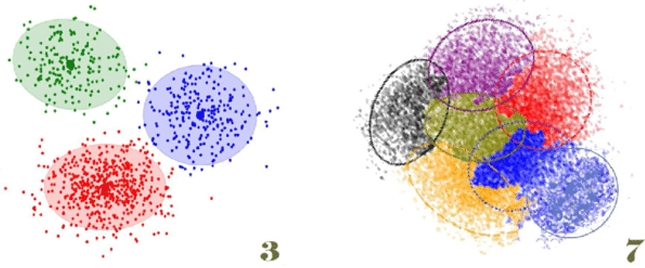
\includegraphics[scale=0.5]{chapter 5/ch5_figure1.jpeg}
    \end{center}
\end{defBox}
\subsection{Aims for Clustering}
\textcolor{cyan}{Labeling} a large set of data samples can be \textcolor{violet}{time-consuming and costly}.\\
Instead, \textcolor{cyan}{clustering} can be used to \textcolor{violet}{find features} that can be used to \textcolor{violet}{label the data for categorization}.\\
\subsection{Applications of Clustering}
\begin{itemize}
    \item \textcolor{cyan}{Similar Size Grouping}: \\
    \underline{e.g.}: Grouping customers of similar sizes together to make "small", "medium" and "large" T-shirts.
    \begin{itemize}
        \item Tailor-made for each person: Too expensive.
        \item One-size-fits-all: Not suitable for everyone.
    \end{itemize}
    \item \textcolor{cyan}{Document Clustering}: \textcolor{violet}{Organizing documents} according to their \textcolor{violet}{content similarities} given a large number of documents to produce a topic hierarchy.
    \item \textcolor{cyan}{Customer Segmentation}: Segmenting customers according to their similarities in marketing to do targeted marketing.
    \item \textcolor{cyan}{Image Segmentation}: \textcolor{violet}{Partitioning a digital image into multiple image segments (image regions)}.
\end{itemize}
\newpage
\textcolor{magenta}{\section{\textbf{K-Means Clustering}}}
\begin{defBox}{Definition 5.2}{K-Means Clustering}
    \raggedright
    \textcolor{cyan}{K-Means Clustering} is an \textcolor{cyan}{unsupervised learning algorithm} that performs the \textcolor{red}{division of data into non-overlapping clusters} sharing similarities and dissimilar to the data belonging to other clusters.\\
    \begin{itemize}
        \item \textcolor{cyan}{No labeled data} in K-Means Clustering unlike in the case of supervised learning.
        \item \textcolor{cyan}{Term 'K' in K-Means} refers to the \textcolor{red}{number of clusters} we need to create for the system (e.g. K = 3 means 3 clusters).
        \item Set of data points is let to be \(D = \{x_1, x_2, \ldots, x_n\}\) where \(x_i = (x_{i1}, x_{i2}, \ldots, x_{id})\) is \(i^{th}\) data point in \(d\)-dimensional space.
        \item Need to \textcolor{red}{specify the desired number of clusters K} to perform the K-Means Clustering.\\
    \end{itemize}
    The K-Means Algorithm \textcolor{cyan}{partitions the given data points into K non-overlapping clusters} where each cluster has a \textcolor{red}{centroid} (\textcolor{cyan}{cluster center}).
    \begin{center}
        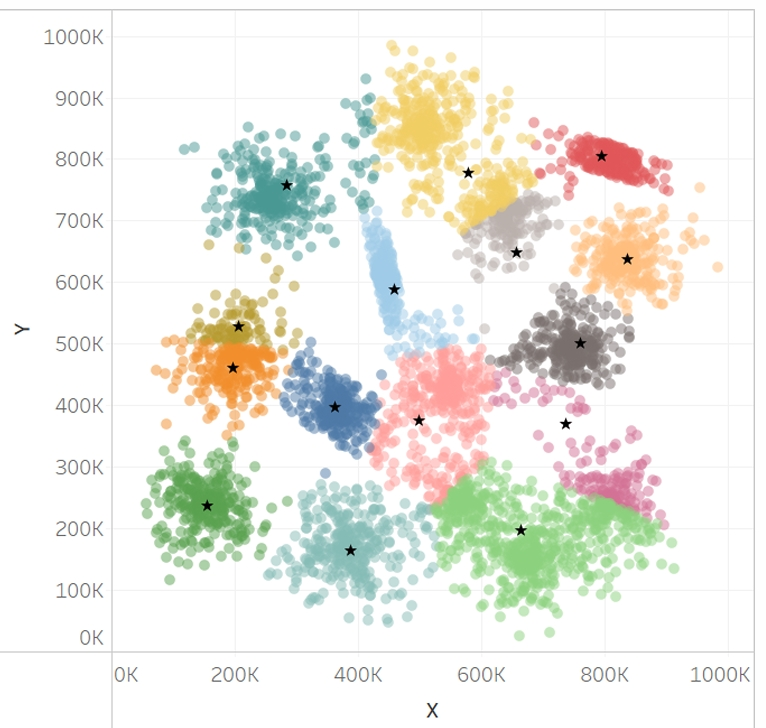
\includegraphics[scale=0.3]{chapter 5/ch5_figure2.jpeg}
    \end{center}
\end{defBox}
\vspace{5mm}
\textbf{\large{\textit{Proof:}}}\\
\vspace{2mm}
\underline{Clustering Algorithm:}\\
\vspace{1mm}
A clustering algorithm must return both a clustering and a center for each cluster.\\
We need to prove the \textcolor{blue}{Sum of Square Error (SSE)} \textcolor{violet}{is minimized} when the center associated with each cluster is the mean/centroid of the set of points assigned to that cluster.\\
Consider the points \(x_1, x_2, \ldots, x_n\) where \(m \geq 1\) and for \( i \in \{1, 2, \ldots, m\}\) where \(x_i\) is an d-dimensional point.\\
\vspace{1mm}
Let \( \bar{x} = \frac{1}{m} \sum_{i=1}^{m} x_i\) be the mean of the points.\\
Let \(x\) be in d-dimensional space an arbitrary point in the same d-dimensional space.\\
\vspace{1mm}
Given \(m\bar{x} = x_1 + x_2 + \ldots + x_m\), we have:
\begin{align*}
    \sum_{i=1}^{m} ||x_i - x|| & = \sum_{i=1}^{m} ||(x_i - \bar{x}) + (\bar{x} - x)||^2 \\
    & = \sum_{i=1}^{m} (||x_i - \bar{x}||^2 + ||\bar{x} - x||^2 + 2(x_i - \bar{x}) \cdot (\bar{x} - x)) \\
    & = \sum_{i=1}^{m} ||x_i - \bar{x}||^2 + \sum_{i=1}^{m} ||\bar{x} - x||^2 + 2\sum_{i=1}^{m} (x_i \cdot \bar{x} - x_i \cdot x - \bar{x} \cdot \bar{x} + \bar{x} \cdot x) \\
    & = \sum_{i=1}^{m} ||x_i - \bar{x}||^2 + m||\bar{x} - x||^2 + 2(m\bar{x} \cdot \bar{x} - m\bar{x} \cdot x - m\bar{x} \cdot \bar{x} + m\bar{x} \cdot x) \\
    & = \sum_{i=1}^{m} ||x_i - \bar{x}||^2 + m||\bar{x} - x||^2 \\
    & \geq \sum_{i=1}^{m} ||x_i - \bar{x}||^2
\end{align*}
\newpage
\underline{Convergence:}\\
\vspace{1mm}
\textcolor{blue}{K-Means Clustering Algorithm} \textcolor{violet}{converges to a local optimum}.\\
To prove convergence of the K-Means Algorithm, we need to show that the loss function is guaranteed to decrease monotonically in each iteration until convergence for the assignment step and for the refitting step.\\
Since the loss function is non-negative, the algorithm will eventually converge when the loss function reaches its local minimum.\\
\vspace{1mm}
Let \(z = (z_1, z_2, \ldots, z_n)\) denote the cluster assignments for the n data points.\\
\vspace{1mm}
\uwave{Assignment Step}\\
We can write down the original loss function as follows:
\[
    L(\mu, z) = \sum_{i=1}^{n} ||x_i - \mu_{z_i}||_2^2 \text{ where } ||\cdot||_2^2 \text{ is square of L2-norm }
\]
Consider a data point \(x_i\) and let \(z_i\) be the cluster assignment from the previous iteration and let \(z_i*\) be the new cluster assignment as:
\[
    z_i^* \in \argmin_{j \in {1, \ldots, K}} ||x_i - \mu_j||_2^2
\]
Let \(z*\) be the new cluster assignments for all the n points. The change in the loss function after this assignment step is:
\[
    L(\mu, z^*) - L(\mu, z) = \sum_{i=1}^{n}(||x_i - \mu_{z_i^*}||_2^2 - ||x_i - \mu_{z_i}||_2^2) \leq 0
\]
The inequality holds by the rule \(z_i*\) is determined to assign \(x_i\) to the nearest cluster center.\\
\vspace{1mm}
\uwave{Refitting Step}\\
We can write down the original loss function \(L(\mu, z)\) as follows:
\[
    L(\mu, z) = \sum_{j=1}^{K} (\sum_{i: z_i = j} ||x_i - \mu_j||_2^2)
\]
Consider the \(j^{th}\) cluster and let \(\mu_j*\) be the new cluster center from the previous iteration and let \(\mu_j\) be the new cluster center as:
\[
    \mu_j^* = \frac{|{i: z_i = j}|}{1} \sum_{i: z_i = j} x_i
\]
Let \(\mu*\) be the new cluster centers for all the K clusters. The change in the loss function after this refitting step is:
\[
    L(\mu^*, z) - L(\mu, z) = \sum_{j=1}^{K} (\sum_{i: z_i = j} ||x_i - \mu_j^*||_2^2 - \sum_{i: z_i = j} ||x_i - \mu_j||_2^2) \leq 0
\]
The inequslity holds because the updated rule of \(\mu_j*\) is determined to minimize the loss function quantity.\\
\textcolor{magenta}{\section{\textbf{K-Means Clustering Algorithm}}}
\begin{wrapfigure}[1]{r}{0.375\textwidth}
    \centering
    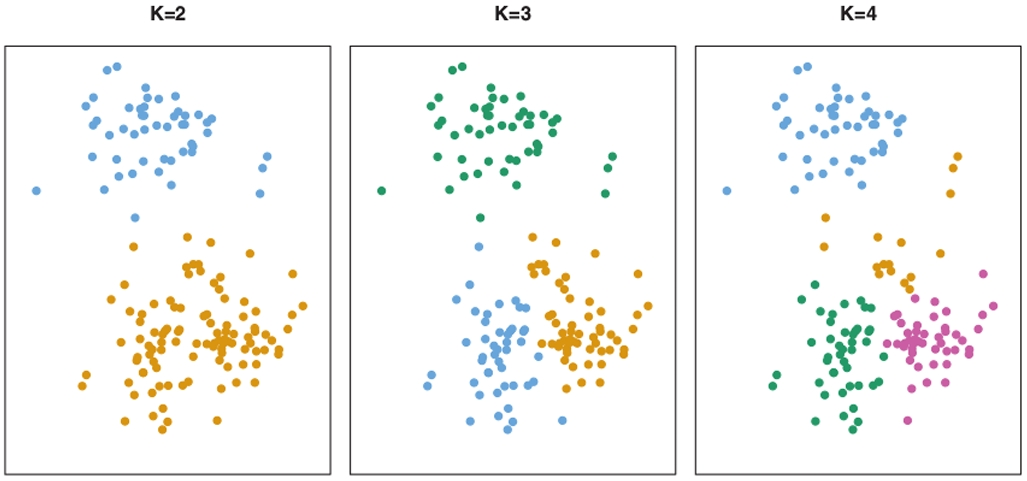
\includegraphics[scale=0.2]{chapter 5/ch5_figure3.jpeg}
\end{wrapfigure}
Here are the steps to implement the K-Means Clustering Algorithm given K:\\
\vspace{2mm}
\begin{enumerate}
    \item \textcolor{violet}{Choose K random data points} (seeds) to be the \textcolor{cyan}{intital centroids} (cluster centers).
    \item Find the \textcolor{cyan}{distances} \textcolor{violet}{between each data point} in our training set \textcolor{violet}{with the K centroids}.
    \item \textcolor{violet}{Assign each data point} to the \textcolor{cyan}{closest centroid} according to the distance found.
    \item \textcolor{cyan}{Re-compute the centroids} using the current cluster assignments.
    \item If a \textcolor{cyan}{convergence criterion} is \textcolor{violet}{NOT met}, repeat steps 2-4.
\end{enumerate}
\vspace{2mm}
\underline{\textbf{Example of K-Means Clustering}}\\
Given the following simplified Mall customers dataset with attributes, age, income (K) and expense score (1-100), where 1 is low spends and 100 is high spends.\\
\begin{center}
    \resizebox{\textwidth}{!}{
        \begin{tabular}{|c|c|c|c|c|c|c|c|c|c|c|c|c|c|c|c|c|c|c|c|c|}
            \hline
            \rowcolor{lightblue}
            \textbf{Person} & 1 & 2 & 3 & 4 & 5 & 6 & 7 & 8 & 9 & 10 & 11 & 12 & 13 & 14 & 15 & 16 & 17 & 18 & 19 & 20 \\  
            \hline
            \textbf{Age} & 19 & 67 & 35 & 60 & 65 & 49 & 70 & 70 & 57 & 68 & 23 & 65 & 27 & 47 & 57 & 43 & 56 & 40 & 37 & 34 \\
            \hline
            \textbf{Income (K)} & 15 & 19 & 24 & 30 & 38 & 42 & 46 & 49 & 54 & 59 & 62 & 63 & 67 & 71 & 75 & 78 & 79 & 87 & 97 & 103 \\
            \hline
            \textbf{Expense Score} & 39 & 14 & 35 & 4 & 35 & 52 & 56 & 55 & 51 & 55 & 41 & 52 & 56 & 9 & 5 & 17 & 35 & 13 & 32 & 23 \\
            \hline
        \end{tabular}
    }
\end{center}
To determine the targeted advertisement and make the marketing budget more efficient, we could K-Means cluster the customers based on their characterisitics (age, income and expense score).\\
\newpage
\begin{wrapfigure}[1]{r}{0.25\textwidth}
    \centering
    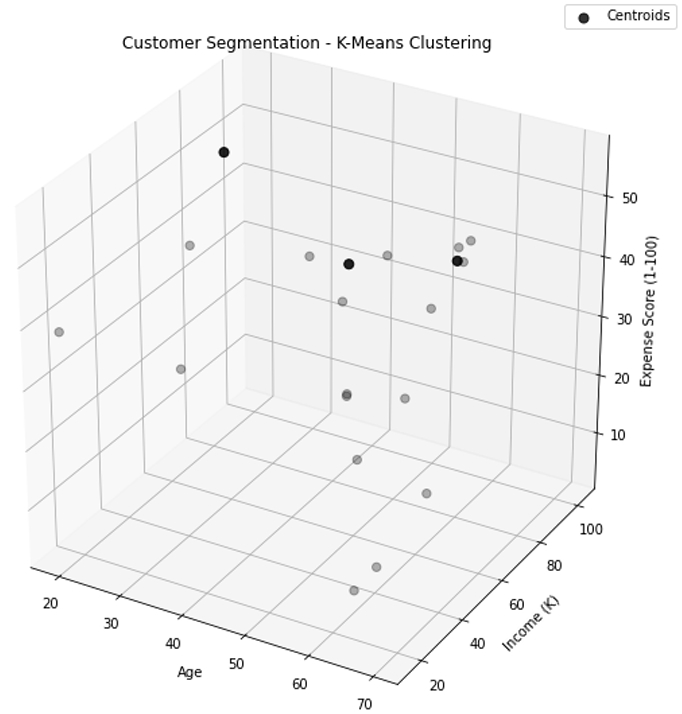
\includegraphics[scale=0.2]{chapter 5/ch5_figure4.jpeg}
\end{wrapfigure}
\uwave{Step 1: Randomly Pick 3 Data Points as Initial Centroids}\\
\begin{itemize}
    \item Centroid 1: (Age = 70, Income (K) = 46, Expense Score = 56)
    \item Centroid 2: (Age = 27, Income (K) = 67, Expense Score = 56)
    \item Centroid 3: (Age = 37, Income (K) = 97, Expense Score = 32)
\end{itemize}
\vspace{2cm}
\uwave{Step 2: Find the Distances Between Each Data Point with the 3 Centroids}\\
Assume the Euclidean Distance Formula is used.
\begin{center}
    \resizebox{\textwidth}{!}{
        \begin{tabular}{|c|c|c|c|c|c|c|c|c|c|c|c|c|c|c|c|c|c|c|c|c|}
            \hline
            \rowcolor{lightblue}
            \textbf{Person} & 1 & 2 & 3 & 4 & 5 & 6 & 7 & 8 & 9 & 10 & 11 & 12 & 13 & 14 & 15 & 16 & 17 & 18 & 19 & 20 \\  
            \hline
            \textbf{Age} & 19 & 67 & 35 & 60 & 65 & 49 & 70 & 70 & 57 & 68 & 23 & 65 & 27 & 47 & 57 & 43 & 56 & 40 & 37 & 34 \\
            \hline
            \textbf{Income (K)} & 15 & 19 & 24 & 30 & 38 & 42 & 46 & 49 & 54 & 59 & 62 & 63 & 67 & 71 & 75 & 78 & 79 & 87 & 97 & 103 \\
            \hline
            \textbf{Expense Score} & 39 & 14 & 35 & 4 & 35 & 52 & 56 & 55 & 51 & 55 & 41 & 52 & 56 & 9 & 5 & 17 & 35 & 13 & 32 & 23 \\
            \hline
            \textbf{DC 1} & 62 & 50 & 46 & 55 & 23 & 22 & 0 & 3 & 16 & 13 & 52 & 18 & 48 & 58 & 60 & 57 & 42 & 67 & 65 & 75 \\
            \hline
            \textbf{DC 2} & 55 & 75 & 49 & 72 & 52 & 34 & 48 & 47 & 33 & 42 & 16 & 38 & 0 & 51 & 60 & 44 & 38 & 49 & 40 & 49 \\
            \hline
            \textbf{DC 3} & 84 & 86 & 73 & 76 & 65 & 60 & 65 & 63 & 51 & 54 & 39 & 48 & 40 & 36 & 40 & 25 & 26 & 22 & 0 & 11 \\
            \hline
        \end{tabular}
    }
\end{center}
where DC1, DC2 and DC3 are the distances between the data points and Centroids 1, 2 and 3 respectively.\\
\vspace{2mm}
\uwave{Step 3: Assign Each Data Point to the Closest Centroid}\\
\begin{center}
    \resizebox{\textwidth}{!}{
        \begin{tabular}{|c|c|c|c|c|c|c|c|c|c|c|c|c|c|c|c|c|c|c|c|c|}
            \hline
            \rowcolor{lightblue}
            \textbf{Person} & 1 & 2 & 3 & 4 & 5 & 6 & 7 & 8 & 9 & 10 & 11 & 12 & 13 & 14 & 15 & 16 & 17 & 18 & 19 & 20 \\  
            \hline
            \textbf{Age} & \cellcolor{lightyellow}{19} & \cellcolor{lightred}{67} & \cellcolor{lightred}{35} & \cellcolor{lightred}{60} & \cellcolor{lightred}{65} & \cellcolor{lightred}{49} & \cellcolor{lightred}{70} & \cellcolor{lightred}{70} & \cellcolor{lightred}{57} & \cellcolor{lightred}{68} & \cellcolor{lightyellow}{23} & \cellcolor{lightred}{65} & \cellcolor{lightyellow}{27} & \cellcolor{lightgreen}{47} & \cellcolor{lightgreen}{57} & \cellcolor{lightgreen}{43} & \cellcolor{lightgreen}{56} & \cellcolor{lightgreen}{40} & \cellcolor{lightgreen}{37} & \cellcolor{lightgreen}{34} \\
            \hline
            \textbf{Income (K)} & \cellcolor{lightyellow}{15} & \cellcolor{lightred}{19} & \cellcolor{lightred}{24} & \cellcolor{lightred}{30} & \cellcolor{lightred}{38} & \cellcolor{lightred}{42} & \cellcolor{lightred}{46} & \cellcolor{lightred}{49} & \cellcolor{lightred}{54} & \cellcolor{lightred}{59} & \cellcolor{lightyellow}{62} & \cellcolor{lightred}{63} & \cellcolor{lightyellow}{67} & \cellcolor{lightgreen}{71} & \cellcolor{lightgreen}{75} & \cellcolor{lightgreen}{78} & \cellcolor{lightgreen}{79} & \cellcolor{lightgreen}{87} & \cellcolor{lightgreen}{97} & \cellcolor{lightgreen}{103} \\
            \hline
            \textbf{Expense Score} & \cellcolor{lightyellow}{39} & \cellcolor{lightred}{14} & \cellcolor{lightred}{35} & \cellcolor{lightred}{4} & \cellcolor{lightred}{35} & \cellcolor{lightred}{52} & \cellcolor{lightred}{56} & \cellcolor{lightred}{55} & \cellcolor{lightred}{51} & \cellcolor{lightred}{55} & \cellcolor{lightyellow}{41} & \cellcolor{lightred}{52} & \cellcolor{lightyellow}{56} & \cellcolor{lightgreen}{9} & \cellcolor{lightgreen}{5} & \cellcolor{lightgreen}{17} & \cellcolor{lightgreen}{35} & \cellcolor{lightgreen}{13} & \cellcolor{lightgreen}{32} & \cellcolor{lightgreen}{23} \\
            \hline
            \textbf{DC 1} & \cellcolor{lightyellow}{62} & \cellcolor{lightred}{50} & \cellcolor{lightred}{46} & \cellcolor{lightred}{55} & \cellcolor{lightred}{23} & \cellcolor{lightred}{22} & \cellcolor{lightred}{0} & \cellcolor{lightred}{3} & \cellcolor{lightred}{16} & \cellcolor{lightred}{13} & \cellcolor{lightyellow}{52} & \cellcolor{lightred}{18} & \cellcolor{lightyellow}{48} & \cellcolor{lightgreen}{58} & \cellcolor{lightgreen}{60} & \cellcolor{lightgreen}{57} & \cellcolor{lightgreen}{42} & \cellcolor{lightgreen}{67} & \cellcolor{lightgreen}{65} & \cellcolor{lightgreen}{75} \\
            \hline
            \textbf{DC 2} & \cellcolor{lightyellow}{55} & \cellcolor{lightred}{75} & \cellcolor{lightred}{49} & \cellcolor{lightred}{72} & \cellcolor{lightred}{52} & \cellcolor{lightred}{34} & \cellcolor{lightred}{48} & \cellcolor{lightred}{47} & \cellcolor{lightred}{33} & \cellcolor{lightred}{42} & \cellcolor{lightyellow}{16} & \cellcolor{lightred}{38} & \cellcolor{lightyellow}{0} & \cellcolor{lightgreen}{51} & \cellcolor{lightgreen}{60} & \cellcolor{lightgreen}{44} & \cellcolor{lightgreen}{38} & \cellcolor{lightgreen}{49} & \cellcolor{lightgreen}{40} & \cellcolor{lightgreen}{49} \\
            \hline
            \textbf{DC 3} & \cellcolor{lightyellow}{84} & \cellcolor{lightred}{86} & \cellcolor{lightred}{73} & \cellcolor{lightred}{76} & \cellcolor{lightred}{65} & \cellcolor{lightred}{60} & \cellcolor{lightred}{65} & \cellcolor{lightred}{63} & \cellcolor{lightred}{51} & \cellcolor{lightred}{54} & \cellcolor{lightyellow}{39} & \cellcolor{lightred}{48} & \cellcolor{lightyellow}{40} & \cellcolor{lightgreen}{36} & \cellcolor{lightgreen}{40} & \cellcolor{lightgreen}{25} & \cellcolor{lightgreen}{26} & \cellcolor{lightgreen}{22} & \cellcolor{lightgreen}{0} & \cellcolor{lightgreen}{11} \\
            \hline
            \textbf{Cluster} & \cellcolor{lightyellow}{2} & \cellcolor{lightred}{1} & \cellcolor{lightred}{1} & \cellcolor{lightred}{1} & \cellcolor{lightred}{1} & \cellcolor{lightred}{1} & \cellcolor{lightred}{1} & \cellcolor{lightred}{1} & \cellcolor{lightred}{1} & \cellcolor{lightred}{1} & \cellcolor{lightyellow}{2} & \cellcolor{lightred}{1} & \cellcolor{lightyellow}{2} & \cellcolor{lightgreen}{3} & \cellcolor{lightgreen}{3} & \cellcolor{lightgreen}{3} & \cellcolor{lightgreen}{3} & \cellcolor{lightgreen}{3} & \cellcolor{lightgreen}{3} & \cellcolor{lightgreen}{3} \\      
            \hline
        \end{tabular}
    }
\end{center}
where DC1, DC2 and DC3 are the distances between the data points and Centroids 1, 2 and 3 respectively.\\
\vspace{2mm}
\uwave{Step 4: Re-Compute the Centroids Using the Current Cluster Assignments}\\
New Centroid 1: 
\[
    x_1 = \frac{67 + 35 + 60 + 65 + 49 + 70 + 70 + 57 + 68 + 65}{10} = 60.6
\]
\[
    x_2 = \frac{19 + 24 + 30 + 38 + 42 + 46 + 49 + 54 + 59 + 63}{10} = 42.4
\]
\[
    x_3 = \frac{14 + 35 + 4 + 35 + 52 + 56 + 55 + 51 + 55 + 52}{10} = 40.9
\]
\vspace{2mm}
New Centroid 2:
\[
    x_1 = \frac{19 + 23 + 27}{3} = 23
\]
\[
    x_2 = \frac{15 + 62 + 67}{3} = 48
\]
\[
    x_3 = \frac{39 + 41 + 56}{3} = 45.3
\]
\vspace{2mm}
New Centroid 3:
\[
    x_1 = \frac{47 + 57 + 43 + 56 + 40 + 37 + 34}{7} = 44.86
\]
\[
    x_2 = \frac{71 + 75 + 78 + 79 + 87 + 97 + 103}{7} = 84.29
\]
\[
    x_3 = \frac{9 + 5 + 17 + 35 + 13 + 32 + 23}{7} = 19.14
\]
\newpage
\begin{figure}[ht]
    \centering
    \begin{tikzpicture}[node distance=5cm]
        \node (ch5_fig5) [rectangle, draw] {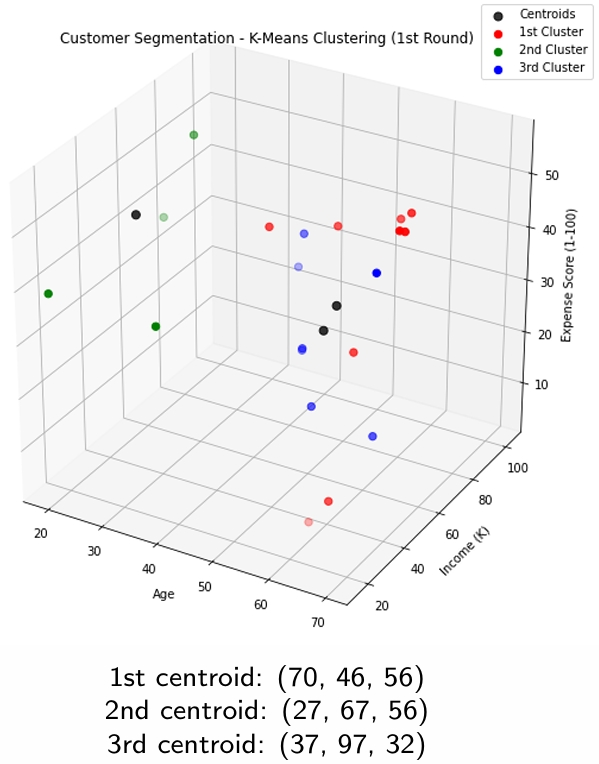
\includegraphics[scale=0.2]{chapter 5/ch5_figure5.jpeg}};
        \node (ch5_fig6) [rectangle, draw, right of=ch5_fig5] {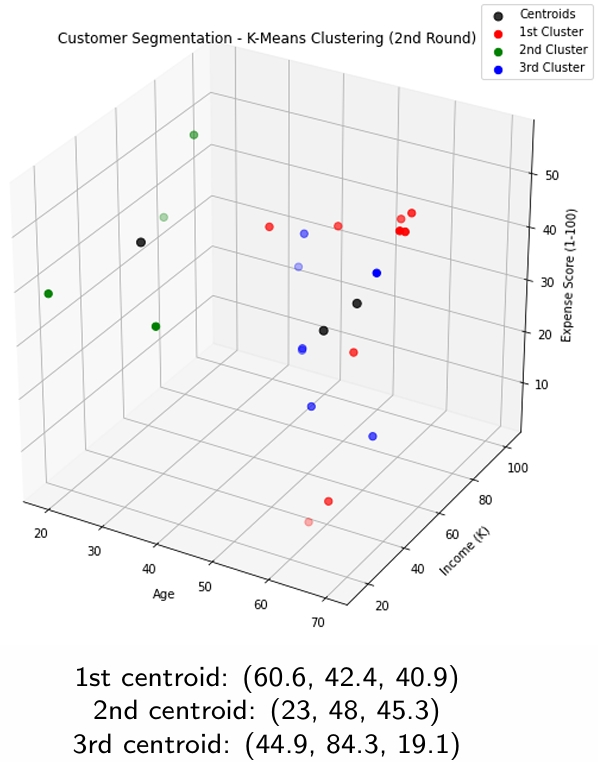
\includegraphics[scale=0.2]{chapter 5/ch5_figure6.jpeg}};
        \node (ch5_fig7) [rectangle, draw, right of=ch5_fig6] {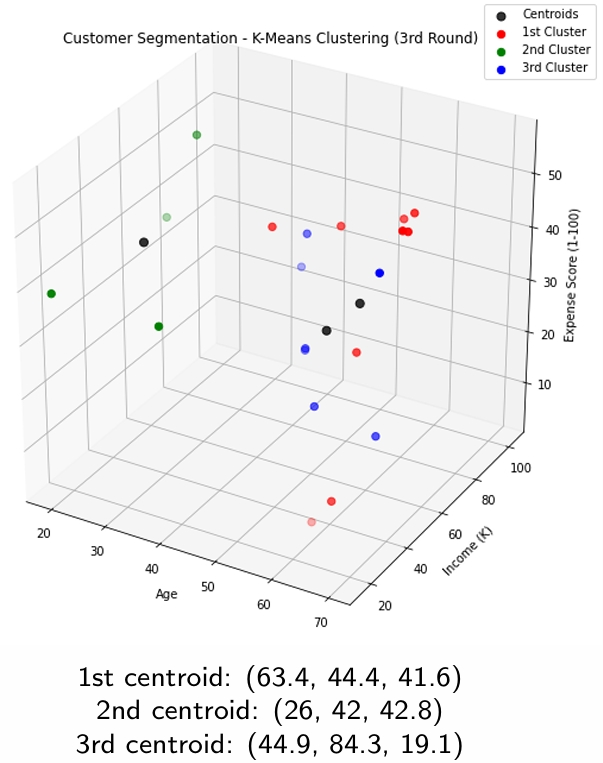
\includegraphics[scale=0.2]{chapter 5/ch5_figure7.jpeg}};
        \node (ch5_fig8) [rectangle, draw, right of=ch5_fig7] {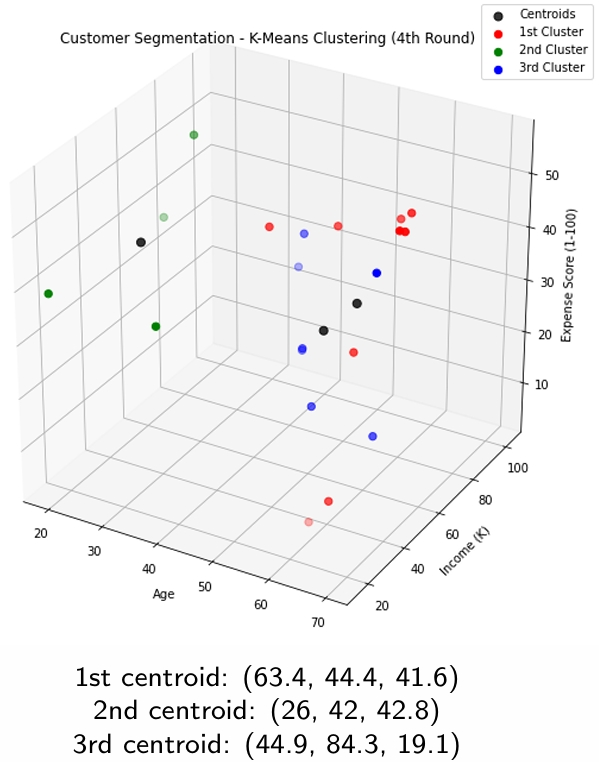
\includegraphics[scale=0.2]{chapter 5/ch5_figure8.jpeg}};

        \node[below of=ch5_fig5, node distance=3.1cm] {Initial Centroids (1st Round)};
        \node[below of=ch5_fig6, node distance=3.1cm] {First Iteration (2nd Round)};
        \node[below of=ch5_fig7, node distance=3.1cm] {Second Iteration (3rd Round)};
        \node[below of=ch5_fig8, node distance=3.1cm] {Final Clusters (4th Round)};

        \draw[->] (ch5_fig5) -- (ch5_fig6);
        \draw[->] (ch5_fig6) -- (ch5_fig7);
        \draw[->] (ch5_fig7) -- (ch5_fig8);
    \end{tikzpicture}
    \caption{Flow Diagram of K-Means Clustering Algorithm}
    \label{ch5_fig1:flow_diagram_k_means}
\end{figure}
\uwave{Step 5: Conclusion}\\
The K-Means Clustering Algorithm has converged to the final clusters.\\
The final clusters are:
\begin{itemize}
    \item Cluster 1: Average Age = \uuline{63.4 years old}, Average Income (K) = \uuline{\textdollar44.4K}, Average Expense Score = \uuline{41.6 out of 100}
    \item Cluster 2: Average Age = \uuline{26 years old}, Average Income (K) = \uuline{\textdollar42K}, Average Expense Score = \uuline{42.8 out of 100}
    \item Cluster 3: Average Age = \uuline{44.9 years old}, Average Income (K) = \uuline{\textdollar84.3K}, Average Expense Score = \uuline{19.1 out of 100}
\end{itemize}
\newpage
\textit{\large{K-Means Clustering Python Code Implementation using Scikit-Learn:}}\\
\begin{lstlisting}[language=Python, basicstyle=\ttfamily\small, keywordstyle=\color{blue}, commentstyle=\color{forestgreen}, stringstyle=\color{red}, showstringspaces=false]
# Import the required libraries
import numpy as np
from sklearn.cluster import KMeans
import matplotlib.pyplot as plt

# Create the training data
data = np.array([[19, 15, 39], [67, 19, 14], [35, 24, 35], [60, 30, 4], [65, 38, 35]
              [49, 42, 52], [70, 46, 56], [70, 49, 55], [57, 54, 51], [68, 59, 55]
              [23, 62, 41], [65, 63, 52], [27, 67, 56], [47, 71, 9], [57, 75, 5]
              [43, 78, 17], [56, 79, 35], [40, 87, 13], [37, 97, 32], [34, 103, 23]])

# Initial Centroids
init_centroids = np.array([[70, 46, 56], [27, 67, 56], [37, 97, 32]])

# Create a KMeans object by specifying:
# - Number of cluster (n_clusters) = 3, Initial Centroids (init) = init_centroids
# - Number of time the k-means algorithm will be run with different centroid seeds (n_init) = 1
# - Maximum number of iterations for the k-means algorithm for a single run (max_iter) = 4
kmeans = KMeans(n_clusters=3, init=init_centroids, n_init=1, max_iter=4)
kmeans.fit(data)                        # Compute k-means clustering
labels = kmeans.predict(data)           # Predict the closest cluster each sample in data belongs to
centroids = kmeans.cluster_centers_     # Resulting centroids
fig = plt.figure(figsize=(10, 10))      # Figure width = 10 inches, height = 10 inches
ax = fig.add_subplot(projection='3d')   # Define 3D axes to plot 3D data into it

# Get boolean arrrays representing entries with labels 0, 1 and 2
a = np.array(labels == 0)
b = np.array(labels == 1)
c = np.array(labels == 2)

# Plot centroids with color = black, size = 50 units, transparency = 0.2 and put a label "Centroids"
ax.scatter(centroids[:, 0], centroids[:, 1], centroids[:, 2],
           c="black", s=50, alpha=0.8, label="Centroids")
# Plot data in the different clusters (1st cluster = red, 2nd cluster = green, 3rd cluster = blue)
ax.scatter(data[a, 0], data[a, 1], data[a, 2], c="red", s=40, label = "1st Cluster")
ax.scatter(data[b, 0], data[b, 1], data[b, 2], c="green", s=40, label = "2nd Cluster")
ax.scatter(data[c, 0], data[c, 1], data[c, 2], c="blue", s=40, label = "3rd Cluster")
ax.legend()                             # Display the legend

# Set the labels for the x, y and z axes
ax.set_xlabel("Age")                    # Put x-axis label as "Age"
ax.set_ylabel("Income (K)")             # Put y-axis label as "Income (K)"
ax.set_zlabel("Expense Score (1-100)")  # Put z-axis label as "Expense Score"
ax.set_title("Customer Segmentation using K-Means Clustering")  # Put figure title

# Output: Text(0.5, 0.92, 'Customer Segmentation - K-Means Clustering')
\end{lstlisting}
\begin{figure}[h]
    \centering
    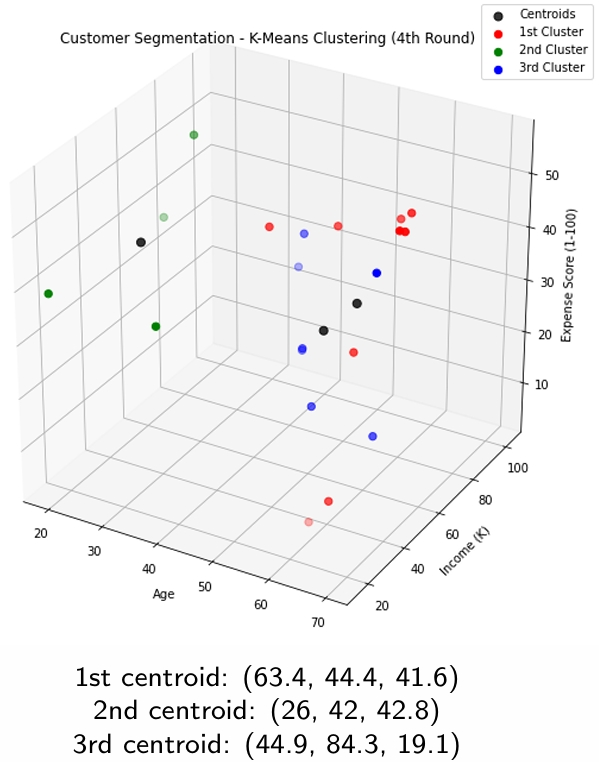
\includegraphics[scale=0.24]{chapter 5/ch5_figure8.jpeg}
    \caption{3D Plot of Customer Segmentation using K-Means Clustering}
\end{figure}
\newpage
\textcolor{magenta}{\section{\textbf{Properties of K-Means Clustering}}}
\subsection{K-Means Stopping Criteria}
\begin{enumerate}
    \item \textcolor{violet}{No/Minimum re-assignments} of data points to different clusters.
    \item \textcolor{violet}{No/Minimum change of centroids} of the clusters.
    \item \textcolor{violet}{Minimum decrease} in the \textcolor{cyan}{Sum of Square Error (SSE)} between successive iterations.
    \[
        SSE = \sum_{j=1}^{K} \sum_{x \in C_j} dist(x, m_j)^2
    \]
    where:\\
    \begin{description}
        \item[\textcolor{brown}{\(C_j\)}]: The \(j^{th}\) cluster.
        \item[\textcolor{brown}{\(m_j\)}]: Centroid of the cluster \(C_j\).
        \item[\textcolor{brown}{\(dist(x, m_j)\)}]: Distance between the data point \(x\) and the centroid \(m_j\).
    \end{description}
\end{enumerate}

\subsection{Clustering Quality}

\fbox{%
    \parbox{\dimexpr\linewidth-2\fboxsep-2\fboxrule}{%
        The quality of the clustering result depends on the algorithm, the distance function, and the application.
    }%
}\\
\vspace{2mm}
For \textcolor{cyan}{high quality clustering}:\\
\begin{itemize}
    \item \textcolor{cyan}{Isolation}: \textcolor{violet}{Maximizes the inter-clusters distances}(distances between the clusters). $\implies$ \hl{Larger isolation = Better clustering}
    \item \textcolor{cyan}{Compactness}: \textcolor{violet}{Minimizes the intra-cluster distances}(distances between the data points in the same cluster).\\
    $\implies$ \hl{Smaller compactness = Better clustering}
\end{itemize}
\begin{figure}[h]
    \centering
    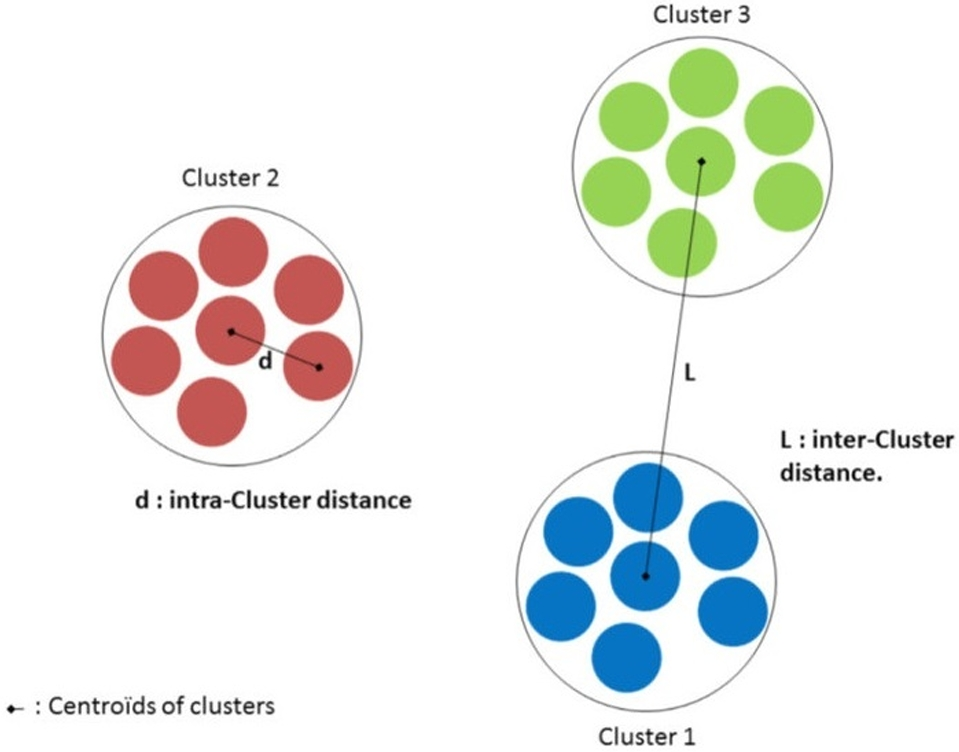
\includegraphics[scale=0.2]{chapter 5/ch5_figure9.jpeg}
\end{figure}
\subsection{K-Estimation for K-Means Clustering}
Elbow Method and Silhouette Score are the two popular methods to estimate the optimal number of clusters K for K-Means Clustering.\\
\begin{itemize}
    \item \textcolor{cyan}{Elbow Method}: \textcolor{violet}{Plot the SSE} for different values of K and \textcolor{violet}{choose the K value} where the \textcolor{cyan}{SSE starts to flatten out}.
    \item \textcolor{cyan}{Silhouette Score}: \textcolor{violet}{Compute the Silhouette Score} for different values of K and \textcolor{violet}{choose the K value} with the \textcolor{cyan}{highest Silhouette Score}.
\end{itemize}
\subsection{Distance Metrics for K-Means Clustering}
The choice of distance metric is crucial for the K-Means Clustering Algorithm, mainly depends on the data type and the domain knowledge.\\
Normally, K-Means Clustering uses the \textcolor{cyan}{Euclidean Distance} as the default distance metric.\\
\begin{itemize}
    \item \textcolor{cyan}{Euclidean Distance}: \textcolor{violet}{Works well for continuous data}.
    \item \textcolor{cyan}{Manhattan Distance}: \textcolor{violet}{Works well for high-dimensional data}.
    \item \textcolor{cyan}{Cosine Similarity}: \textcolor{violet}{Works well for text data}.
    \item \textcolor{cyan}{Hamming Distance}: \textcolor{violet}{Works well for binary data}.
\end{itemize}
\subsection{Standardization for K-Means Clustering}
It is recommended that the data should be standardized with a \textcolor{cyan}{mean of 0} and a \textcolor{cyan}{standard deviation of 1} because every dataset has features with different measurement units like age or income.\\
Clustering algorithms including K-Means use \textcolor{cyan}{distance-based measurements} to determine the similarity between data points.\\
\newpage
\textcolor{magenta}{\section{\textbf{Pros and Cons of K-Means Clustering}}}
\subsection{Pros of K-Means Clustering}
\begin{itemize}
    \item \textcolor{cyan}{Simple and Easy to Implement}: K-Means Clustering is \textcolor{violet}{easy to understand and implement}.
    \item \textcolor{cyan}{Fast and Efficient}: K-Means Clustering is \textcolor{violet}{computationally faster and efficient} given K and the number of iterations is small.
    \item \textcolor{cyan}{Scalable}: K-Means Clustering can \textcolor{violet}{handle large datasets} with ease.
    \item \textcolor{cyan}{Interpretability}: K-Means Clustering produces clusters that are \textcolor{violet}{easy to interpret}.
    \item \textcolor{cyan}{Versatile}: K-Means Clustering can be used for various types of data.
\end{itemize}
\subsection{Cons of K-Means Clustering}
\begin{itemize}
    \item \textcolor{cyan}{Mean Requirement}: K-Means Clustering is \textcolor{violet}{applicable if the mean is defined}.
    \item \textcolor{cyan}{Requires Predefined K}: K-Means Clustering \textcolor{violet}{requires the user to specify K}.
    \item \textcolor{cyan}{Sensitive to Outliers}: K-Means Clustering is \textcolor{violet}{sensitive to outliers} and may result in poor clustering.
    \item \textcolor{cyan}{Sensitive to Initial Centroids}: K-Means Clustering is \textcolor{violet}{sensitive to the initial centroids} and may result in different clusters.
    \item \textcolor{cyan}{Non-Convex Clusters}: K-Means Clustering \textcolor{violet}{cannot handle non-convex clusters}.
\end{itemize}
\textcolor{magenta}{\section{\textbf{Weaknesses of K-Means Clustering}}}
\begin{enumerate}
    \item \textcolor{cyan}{Sensitive to Outliers}
    \begin{itemize}
        \item Outliers (Data points that are very far away from the other data points) could cause errors in the  data recording/some special data points with very different values.
        \item We want desirable clustering instead of undesirable clustering with outliers. \\
        \begin{figure}[h]
            \centering
            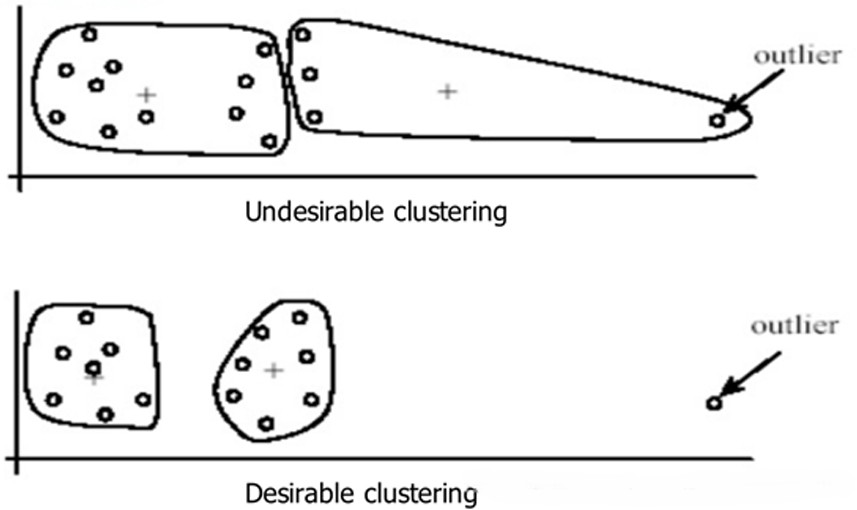
\includegraphics[scale=0.25]{chapter 5/ch5_figure10.jpeg}
        \end{figure}
        There are two ways to handle outliers:
        \begin{enumerate}
            \item \textcolor{cyan}{Remove some Data Points} in the clustering process much \textcolor{violet}{further away from the centroids than other data points}.\\
            (We want to monitor these possible outliers over a few iterations and then decide to remove them).
            \item Perform \textcolor{cyan}{Random Sampling}: We only \textcolor{violet}{choose a small subset of the data points} in sampling, the chance of \textcolor{violet}{selecting an outlier is very small}.\\
            (Assign the rest of the data points to the clusters by distance/similarity comparison/classification).
        \end{enumerate}
    \end{itemize}
    \item \textcolor{cyan}{Sensitive to Initial Seeds}
    \begin{itemize}
        \item If we use seeds that are not-so-good, the algorithm produces a bad clustering result.
        \begin{figure}[h]
            \centering
            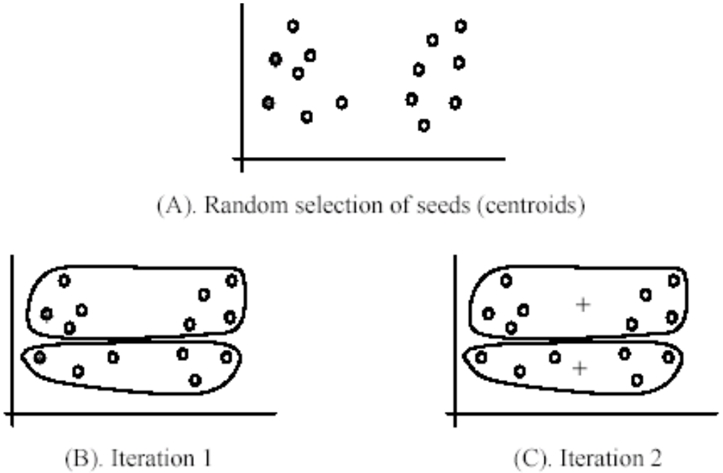
\includegraphics[scale=0.25]{chapter 5/ch5_figure11.jpeg}
        \end{figure}
        \newpage
        \item If we use different seeds, the algorithm produces good clustering results.
        \begin{figure}[h]
            \centering
            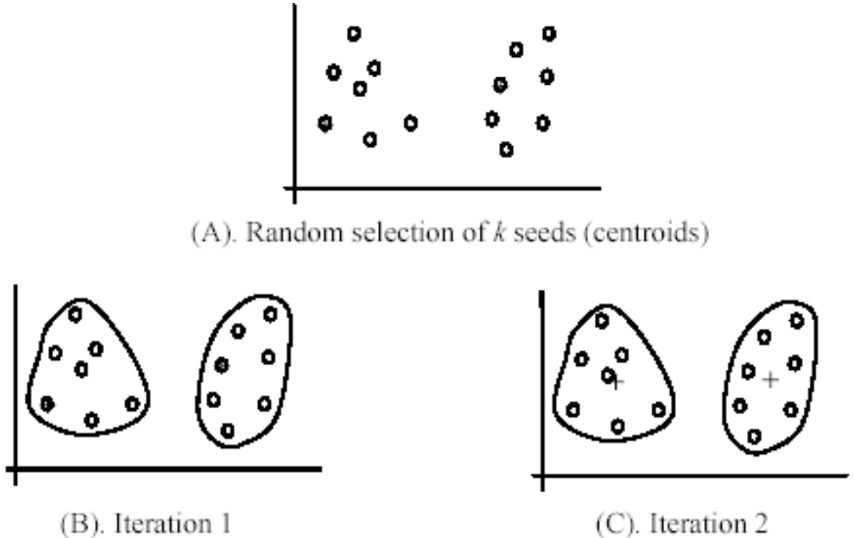
\includegraphics[scale=0.25]{chapter 5/ch5_figure12.jpeg}
        \end{figure}
    \end{itemize}
    
    \item \textcolor{cyan}{Not suitable for discovering clusters} that are \hl{not hyper-ellipsoids/hyper-spheres}.
    \begin{figure}[h]
        \centering
        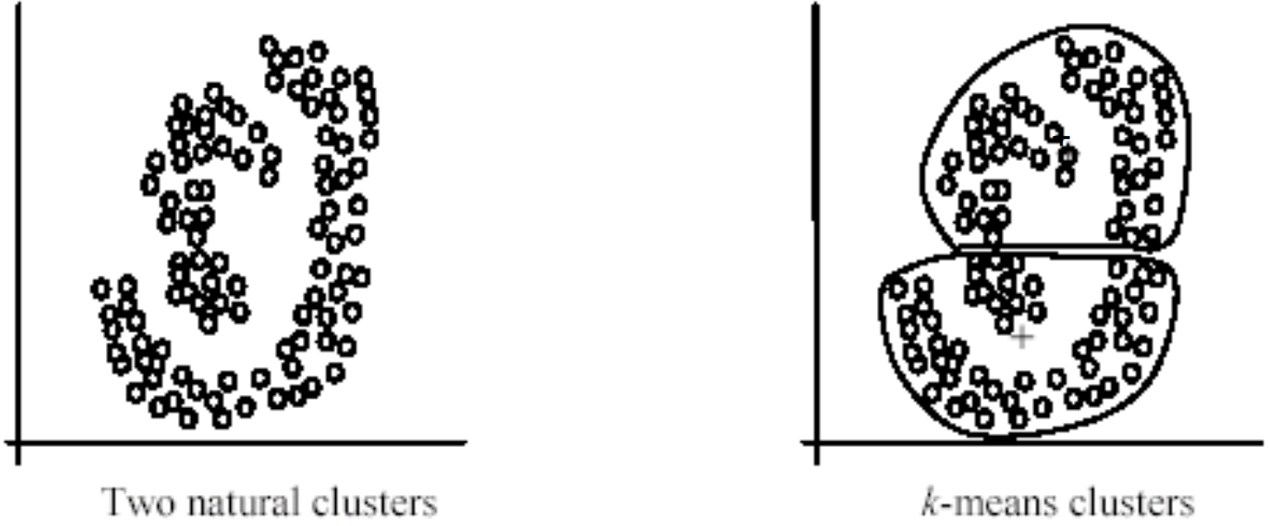
\includegraphics[scale=0.25]{chapter 5/ch5_figure13.jpeg}
    \end{figure}
\end{enumerate}
\textcolor{magenta}{\section{\textbf{Dimension Reduction using PCA}}}
\subsection{Introduction to Principal Component Analysis (PCA)}
\begin{defBox}{Definition 5.7}{Principal Component Analysis (PCA)}
    \raggedright
    \textcolor{cyan}{Principal Component Analysis (PCA)} is a \textcolor{cyan}{dimension-reduction method} that can be used to \textcolor{red}{reduce a large set of variables (normally correlated) into a smaller set of principal components (uncorrelated)} containing most of the information in the original dataset.\\
    \begin{itemize}
        \item Basically a \textcolor{red}{projection of some higher dimensional data into a lower dimensional space}.
        \item One of the easiest, most intuitive and most frequently used methods for dimensionality reduction, projecting data onto its orthogonal feature subspace.
        \item \textcolor{red}{Common in practice to apply PCA before applying K-Means Clustering} to reduce the dimensionality of the data.
        \item Improves the clustering results in practice.
    \end{itemize}
\end{defBox}
To \textcolor{violet}{retain as much information as possible}, we need to find the longest axis of the object and after that turn the object around this axis so that we can find the second longest axis in PCA.\\
PCA can be done by calculating the \textcolor{cyan}{eigenvectors of the covariance matrix} and then use the \(n\) eigenvectors with the \textcolor{violet}{biggest eigenvalues} to project the object into \(n\)-dimensional space.\\
\begin{figure}[h]
    \centering
    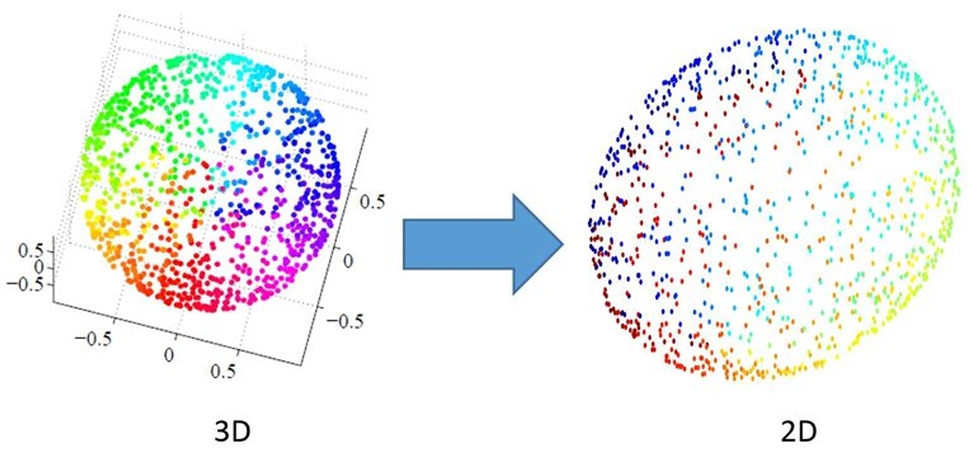
\includegraphics[scale=0.3]{chapter 5/ch5_figure14.jpeg}
\end{figure}
\newpage
\subsection{Steps to Perform PCA}
Here are the steps to perform PCA:
\begin{enumerate}
    \item Take the whole dataset consisting of \textcolor{violet}{\(d+1\) dimensions} and ignore the labels such that our new dataset becomes \textcolor{violet}{\(d\) dimensions}.
    \item Compute the \textcolor{cyan}{means for every dimension} of the whole dataset.
    \item Compute the \textcolor{cyan}{covariance matrix} of the whole dataset.
    \item Compute the \textcolor{cyan}{eigenvectors and the corresponding eigenvalues} of the covariance matrix.
    \item \textcolor{cyan}{Sort the eigenvectors by decreasing eigenvalues} and choose \(k\) eigenvectors with the largest eigenvalues to form a \(d \times k\) dimensional matrix \(\mathbf{W}\).
    \item Use the \(d \times k\) matrix \(\mathbf{W}\) to transform the samples onto the new subspace.
\end{enumerate}
\vspace{2mm}
\underline{\textbf{Example of PCA}}\\
Let our data be the scores of 5 students:
\begin{center}
    \begin{tabular}{|c|c|c|c|c|}
        \hline
        \rowcolor{lightblue}
        \textbf{Student} & \textbf{COMP2011} & \textbf{COMP2012} & \textbf{COMP2211} & \textbf{Label}\\
        \hline
        \textbf{1} & 90 & 60 & 90 & ? \\
        \hline
        \textbf{2} & 90 & 90 & 30 & ? \\
        \hline
        \textbf{3} & 60 & 60 & 60 & ? \\
        \hline
        \textbf{4} & 60 & 60 & 90 & ? \\
        \hline
        \textbf{5} & 30 & 30 & 30 & ? \\
        \hline
    \end{tabular}
\end{center}
\uwave{Step 1: Take the Whole Dataset Consisting of \(d+1\) Dimensions \& Ignore the Labels such that the New Dataset Becomes \(d\) Dimensions}\\
The dataset forms a 2D matrix:
\[
    M = \begin{bmatrix}
        90 & 60 & 90\\
        90 & 90 & 30\\
        60 & 60 & 60\\
        60 & 60 & 90\\
        30 & 30 & 30
    \end{bmatrix}
\]
\uwave{Step 2: Compute the Means for Every Dimension of the Whole Dataset}\\
1st Dimension Mean: \(\mu_1 = \frac{90 + 90 + 60 + 60 + 30}{5} = 66\)\\
\vspace{1mm}
2nd Dimension Mean: \(\mu_2 = \frac{60 + 90 + 60 + 60 + 30}{5} = 60\)\\
\vspace{1mm}
3rd Dimension Mean: \(\mu_3 = \frac{90 + 30 + 60 + 90 + 30}{5} = 60\)\\
\vspace{2mm}
Mean of the whole dataset:
\[
    \bar{M} = \begin{bmatrix}
        66 & 60 & 60
    \end{bmatrix}
\]
\uwave{Step 3: Compute the Covariance Matrix of the Whole Dataset}\\
The covariance of the two variables \(X\) and \(Y\) is given by:
\[
    Cov(X, Y) = \frac{\sum_{i=1}^{n} (X_i - \bar{x})(Y_i - \bar{y})}{n-1}
\]
Using the formula, we can compute the covariance matrix of the dataset whcih is a \(3 \times 3\) matrix:\\
\vspace{2mm}
\( cov(\text{COMP2011, COMP2011}) = \frac{(90-66)(90-66) + (90-66)(90-66) + (60-66)(60-66) + (60-66)(60-66) + (30-66)(30-66)}{5-1} = 630 \)\\
\( cov(\text{COMP2011, COMP2012}) = \frac{(90-66)(60-60) + (90-66)(90-60) + (60-66)(60-60) + (60-66)(60-60) + (30-66)(30-60)}{5-1} = 450 \)\\
\( cov(\text{COMP2011, COMP2211}) = \frac{(90-66)(90-60) + (90-66)(30-60) + (60-66)(60-60) + (60-66)(90-60) + (30-66)(30-60)}{5-1} = 225 \)\\
\( cov(\text{COMP2012, COMP2011}) = \frac{(60-60)(90-66) + (90-60)(90-66) + (60-60)(60-66) + (60-60)(60-66) + (30-60)(30-66)}{5-1} = 450 \)\\
\( cov(\text{COMP2012, COMP2012}) = \frac{(60-60)(60-60) + (90-60)(90-60) + (60-60)(60-60) + (60-60)(60-60) + (30-60)(30-60)}{5-1} = 450 \)\\
\( cov(\text{COMP2012, COMP2211}) = \frac{(60-60)(90-60) + (90-60)(30-60) + (60-60)(60-60) + (60-60)(90-60) + (30-60)(30-60)}{5-1} = 0 \)\\
\( cov(\text{COMP2211, COMP2011}) = \frac{(90-60)(90-66) + (30-60)(90-66) + (60-60)(60-66) + (90-60)(60-66) + (30-60)(30-66)}{5-1} = 225 \)\\
\( cov(\text{COMP2211, COMP2012}) = \frac{(90-60)(60-60) + (30-60)(90-60) + (60-60)(60-60) + (90-60)(60-60) + (30-60)(30-60)}{5-1} = 0 \)\\
\( cov(\text{COMP2211, COMP2211}) = \frac{(90-60)(90-60) + (30-60)(30-60) + (60-60)(60-60) + (90-60)(90-60) + (30-60)(30-60)}{5-1} = 900 \)\\
\vspace{2mm}
$\therefore$ The covariance matrix of the dataset is:
\[
    C = \begin{bmatrix}
        630 & 450 & 225\\
        450 & 450 & 0\\
        225 & 0 & 900
    \end{bmatrix}
\]
Observations Based on the Covariance Matrix:
\begin{itemize}
    \item The covariance between COMP2011 and COMP2012 is +450 \& the covariance between COMP2011 and COMP2211 is +225:\\
    \textcolor{red}{The scores tend to co-vary in a positive way} (The scores on COMP2011 go up, scores on COMP2012 and COMP2211 also tend to go up and vice versa).
    \item The covariance between COMP2012 and COMP2211 is 0:\\
    \textcolor{red}{The scores tend to be no predictable relationship} between the movement of the scores on COMP2012 and COMP2211.
\end{itemize}
\newpage
\uwave{Step 4: Compute the Eigenvectors and the Corresponding Eigenvalues of the Covariance Matrix}\\
Let \(\mathbf{A}\) be a square matrix, \(\mathbf{v}\) be a vector and \(\lambda\) be a scalar satisfies \(\mathbf{Av}= \lambda \mathbf{v}\).\\
\(\Rightarrow\) Eigenvalue \(\lambda\) is associated with the eigenvector \(\mathbf{v}\) of the matrix \(\mathbf{A}\).\\
The eigenvalues of \(\mathbf{A}\) are the roots of the characteristic equation: \(\text{det}(\mathbf{A} - \lambda \mathbf{I}) = 0\).\\
\vspace{2mm}
Calculating \(\text{det}(\mathbf{A} - \lambda \mathbf{I})\) first where \(\mathbf{I}\) is the identity matrix:
\[
    \text{det}(\mathbf{A} - \lambda \mathbf{I}) = \text{det}(\begin{bmatrix}
        630 & 450 & 225\\
        450 & 450 & 0\\
        225 & 0 & 900
    \end{bmatrix}
    - \lambda \begin{bmatrix}
        1 & 0 & 0\\
        0 & 1 & 0\\
        0 & 0 & 1
    \end{bmatrix})
    = \text{det}(\begin{bmatrix}
        630-\lambda & 450 & 225\\
        450 & 450-\lambda & 0\\
        225 & 0 & 900-\lambda
    \end{bmatrix})
\]
Now equating the determinant to 0: \(-\lambda^3 + 1980\lambda^2 - 1002375\lambda + 50118750 = 0\).\\
Solving the equation for the value of \(\lambda\), we get the eigenvalues of the covariance matrix: \( \lambda_1 = 56.025\), \( \lambda_2 = 786.388\), \( \lambda_3 = 1137.587\).\\
\vspace{2mm}
After solving for the eigenvalues, we can find the eigenvectors by solving the equation \(\mathbf{Av} = \lambda \mathbf{v}\).\\
The eigenvectors of the covariance matrix are:
\[
    \mathbf{v_1} = \begin{bmatrix}
        0.6487899\\
        -0.74104991\\
        -0.17296443
    \end{bmatrix}, \mathbf{v_2} = \begin{bmatrix}
        -0.3859988\\
        -0.51636642\\
        0.7644414
    \end{bmatrix}, \mathbf{v_3} = \begin{bmatrix}
        -0.65580225\\
        -0.4291978\\
        -0.62105769
    \end{bmatrix}
\]
\uwave{Step 5: Sort Eigenvectors by Decreasing Eigenvalues \& Choose \(k\) Eigenvectors with Largest Eigenvalues to Form a \(d \times k\) Dimensional Matrix \(\mathbf{W}\)}\\
After sorting the eigenvectors by decreasing eigenvalues, we get: \(\lambda_3 > \lambda_2 > \lambda_1\).\\
We want to reduce the 3D dataset to 2D, so we choose the first 2 eigenvectors with the largest eigenvalues to construct the \(d \times k\) matrix \(\mathbf{W}\):
\[
    \mathbf{W} = \begin{bmatrix}
        -0.65580225 & -0.3859988\\
        -0.4291978 & -0.51636642\\
        -0.62105769 & 0.7644414
    \end{bmatrix}
\]
\uwave{Step 6: Use the \(d \times k\) Matrix \(\mathbf{W}\) to Transform the Samples onto the New Subspace}\\
We use the matrix \(\mathbf{W}\) to transform the samples onto the new subspace via the equation: \(\mathbf{y} = \mathbf{xW}\).\\
\[
    \therefore \mathbf{y} = \begin{bmatrix}
        90 & 60 & 90\\
        90 & 90 & 30\\
        60 & 60 & 60\\
        60 & 60 & 90\\
        30 & 30 & 30
    \end{bmatrix} \begin{bmatrix}
        -0.65580225 & -0.3859988\\
        -0.4291978 & -0.51636642\\
        -0.62105769 & 0.7644414
    \end{bmatrix} = \underline{\underline{\begin{bmatrix}
        -140.67 & 3.08\\
        -116.28 & -58.28\\
        -102.36 & -8.28\\
        -121.00 & 14.66\\
        -51.18 & -4.14
    \end{bmatrix}}}
\]
The transformed dataset is a 5x2 matrix.\\
The transformed dataset can be used for clustering using K-Means Clustering Algorithm.\\
\newpage
\textit{\large{PCA Python Code Implementation using NumPy:}}\\
\begin{lstlisting}[language=Python, basicstyle=\ttfamily\small, keywordstyle=\color{blue}, commentstyle=\color{forestgreen}, stringstyle=\color{red}, showstringspaces=false]
import numpy as np # Import NumPy library

# Create the original dataset
x = np.array([[90, 60, 90], [90, 90, 30], [60, 60, 60], [60, 60, 90], [30, 30, 30]])

# Compute the covariance matrix of the dataset
covariance_matrix = np.cov(x, rowvar = False, bias = False) 
print("Covariance Matrix:\n", covariance_matrix)

# Compute the eigenvalues and eigenvectors of the covariance matrix
eigenvalues, eigenvectors = np.linalg.eig(covariance_matrix) 

# Sort the eigenvectors by decreasing eigenvalues
sorted_index = np.argsort(eigenvalues)[::-1]
sorted_eigenvalue = eigenvalues[sorted_index]
sorted_eigenvectors = eigenvectors[:, sorted_index]
print("Eigenvalues:\n", sorted_eigenvalue)
print("Eigenvectors:\n", sorted_eigenvectors)

# Choose the first 2 eigenvectors with the largest eigenvalues to form a 3x2 transformation matrix
W = np.array([sorted_eigenvectors[:, 0], sorted_eigenvectors[:, 1]]).T
print("Transformation Matrix:\n", W)

# Transform the original dataset into the new subspace
y = x.dot(W)
print("Transformed Dataset:\n", y)



# Output:

# Covariance Matrix:
#  [[630. 450. 225.]
#  [450. 450.   0.]
#  [225.   0. 900.]]
# Eigenvalues:
#  [1137.5874413   786.38798335   56.02457535]
# Eigenvectors:
#  [[-0.65580225 -0.3859988   0.6487899 ]
#  [-0.4291978  -0.51636642 -0.74104991]
#  [-0.62105769  0.7644414  -0.17296443]]
# Transformation Matrix:
#  [[-0.65580225 -0.3859988 ]
#  [-0.4291978  -0.51636642]
#  [-0.62105769  0.7644414 ]]
# Transformed Dataset:
#  [[-140.6692628     3.07784927]
#  [-116.28173533  -58.27962721]
#  [-102.36346447   -8.27542884]
#  [-120.99519515   14.65781313]
#  [ -51.18173223   -4.13771442]]
\end{lstlisting}
\newpage
\textbf{\textcolor{purple}{\Large{Practice Problem}}}\\
\textbf{Question}:\\
Given 4 types of medicines and each has two attributes (weight and PH index) as shown in the table below.\\
\begin{center}
    \begin{tabular}{|c|c|c|c|c|}
        \hline
        \rowcolor{lightblue}
        \textbf{Medicine} & \textbf{A} & \textbf{B} & \textbf{C} & \textbf{D}\\
        \hline
        \textbf{Weight Index} & 1 & 2 & 4 & 5 \\
        \hline
        \textbf{pH Index} & 1 & 1 & 3 & 4 \\
        \hline
    \end{tabular}
\end{center} 
Group these medicines into \(K=2\) group using K-Means Clustering Algorithm.\\
Use \(1,1\) and \(2,1\) as the initial centroids and performing K-Means Clustering until there is no re-assignment of data points to different clusters.\\
\vspace{2mm}
\textbf{Answer}:\\
\uwave{Step 1: Use the 2 Given Data Points as the Initial Centroids}\\
\begin{itemize}
    \item 1st Centroid: (1, 1)
    \item 2nd Centroid: (2, 1)
\end{itemize}
\uwave{Step 2: Find the Distances Between the Data Points and the Centroids}\\
Assume the Euclidean Distance as the distance metric.\\
\begin{center}
    \begin{tabular}{|c|c|c|c|c|}
        \hline
        \rowcolor{lightblue}
        \textbf{Medicine} & \textbf{A} & \textbf{B} & \textbf{C} & \textbf{D}\\
        \hline
        \textbf{Weight Index} & 1 & 2 & 4 & 5 \\
        \hline
        \textbf{pH Index} & 1 & 1 & 3 & 4 \\
        \hline
        \textbf{Distance from (1, 1)} & 0 & 1 & 3.6 & 5 \\
        \hline
        \textbf{Distance from (2, 1)} & 1 & 0 & 2.8 & 4.2 \\
        \hline
    \end{tabular}
\end{center}
\uwave{Step 3: Assign the Data Points to the Nearest Centroids}\\
\begin{center}
    \begin{tabular}{|c|c|c|c|c|}
        \hline
        \rowcolor{lightblue}
        \textbf{Medicine} & \textbf{A} & \textbf{B} & \textbf{C} & \textbf{D}\\
        \hline
        \textbf{Weight Index} & \cellcolor{lightyellow}{1} & \cellcolor{lightred}{2} & \cellcolor{lightred}{4} & \cellcolor{lightred}{5} \\
        \hline
        \textbf{pH Index} & \cellcolor{lightyellow}{1} & \cellcolor{lightred}{1} & \cellcolor{lightred}{3} & \cellcolor{lightred}{4} \\
        \hline
        \textbf{Distance from (1, 1)} & \cellcolor{lightyellow}{0} & \cellcolor{lightred}{1} & \cellcolor{lightred}{3.6} & \cellcolor{lightred}{5} \\
        \hline
        \textbf{Distance from (2, 1)} & \cellcolor{lightyellow}{1} & \cellcolor{lightred}{0} & \cellcolor{lightred}{2.8} & \cellcolor{lightred}{4.2} \\
        \hline
        \textbf{Cluster} & \cellcolor{lightyellow}{1} & \cellcolor{lightred}{2} & \cellcolor{lightred}{2} & \cellcolor{lightred}{2} \\
        \hline
    \end{tabular}
\end{center}
\uwave{Step 4: Re-compute the Centroids of the Clusters}\\
\begin{itemize}
    \item New 1st Centroid: (1, 1)
    \item New 2nd Centroid: \((\frac{2+4+5}{3}, \frac{1+3+4}{3}) = (3.67, 2.67)\)
\end{itemize}
\uwave{Step 5: Find the Distances Between the Data Points and the New Centroids}\\
Assume the Euclidean Distance as the distance metric.\\
\begin{center}
    \begin{tabular}{|c|c|c|c|c|}
        \hline
        \rowcolor{lightblue}
        \textbf{Medicine} & \textbf{A} & \textbf{B} & \textbf{C} & \textbf{D}\\
        \hline
        \textbf{Weight Index} & 1 & 2 & 4 & 5 \\
        \hline
        \textbf{pH Index} & 1 & 1 & 3 & 4 \\
        \hline
        \textbf{Distance from (1, 1)} & 0 & 1 & 3.6 & 5 \\
        \hline
        \textbf{Distance from (3.67, 2.67)} & 3.1 & 2.4 & 0.5 & 1.9 \\
        \hline
    \end{tabular}
\end{center}
\uwave{Step 6: Assign the Data Points to the Nearest Centroids}\\
\begin{center}
    \begin{tabular}{|c|c|c|c|c|}
        \hline
        \rowcolor{lightblue}
        \textbf{Medicine} & \textbf{A} & \textbf{B} & \textbf{C} & \textbf{D}\\
        \hline
        \textbf{Weight Index} & \cellcolor{lightyellow}{1} & \cellcolor{lightyellow}{2} & \cellcolor{lightred}{4} & \cellcolor{lightred}{5} \\
        \hline
        \textbf{pH Index} & \cellcolor{lightyellow}{1} & \cellcolor{lightyellow}{1} & \cellcolor{lightred}{3} & \cellcolor{lightred}{4} \\
        \hline
        \textbf{Distance from (1, 1)} & \cellcolor{lightyellow}{0} & \cellcolor{lightyellow}{1} & \cellcolor{lightred}{3.6} & \cellcolor{lightred}{5} \\
        \hline
        \textbf{Distance from (3.67, 2.67)} & \cellcolor{lightyellow}{3.1} & \cellcolor{lightyellow}{2.4} & \cellcolor{lightred}{0.5} & \cellcolor{lightred}{1.9} \\
        \hline
        \textbf{Cluster} & \cellcolor{lightyellow}{1} & \cellcolor{lightyellow}{1} & \cellcolor{lightred}{2} & \cellcolor{lightred}{2} \\
        \hline
    \end{tabular}
\end{center}
\uwave{Step 7: Re-compute the Centroids of the Clusters}\\
\begin{itemize}
    \item New 1st Centroid: \((\frac{1+2}{2}, \frac{1+1}{2}) = (1.5, 1)\)
    \item New 2nd Centroid: \((\frac{4+5}{2}, \frac{3+4}{2}) = (4.5, 3.5)\)
\end{itemize}
\uwave{Step 8: Find the Distances Between the Data Points and the New Centroids}\\
Assume the Euclidean Distance as the distance metric.\\
\begin{center}
    \begin{tabular}{|c|c|c|c|c|}
        \hline
        \rowcolor{lightblue}
        \textbf{Medicine} & \textbf{A} & \textbf{B} & \textbf{C} & \textbf{D}\\
        \hline
        \textbf{Weight Index} & 1 & 2 & 4 & 5 \\
        \hline
        \textbf{pH Index} & 1 & 1 & 3 & 4 \\
        \hline
        \textbf{Distance from (1.5, 1)} & 0.5 & 0.5 & 3.2 & 4.6 \\
        \hline
        \textbf{Distance from (4.5, 3.5)} & 4.3 & 3.5 & 0.7 & 0.7 \\
        \hline
    \end{tabular}
\end{center}
\newpage
\uwave{Step 9: Assign the Data Points to the Nearest Centroids}\\
\begin{center}
    \begin{tabular}{|c|c|c|c|c|}
        \hline
        \rowcolor{lightblue}
        \textbf{Medicine} & \textbf{A} & \textbf{B} & \textbf{C} & \textbf{D}\\
        \hline
        \textbf{Weight Index} & \cellcolor{lightyellow}{1} & \cellcolor{lightyellow}{2} & \cellcolor{lightred}{4} & \cellcolor{lightred}{5} \\
        \hline
        \textbf{pH Index} & \cellcolor{lightyellow}{1} & \cellcolor{lightyellow}{1} & \cellcolor{lightred}{3} & \cellcolor{lightred}{4} \\
        \hline
        \textbf{Distance from (1.5, 1)} & \cellcolor{lightyellow}{0.5} & \cellcolor{lightyellow}{0.5} & \cellcolor{lightred}{3.2} & \cellcolor{lightred}{4.6} \\
        \hline
        \textbf{Distance from (4.5, 3.5)} & \cellcolor{lightyellow}{4.3} & \cellcolor{lightyellow}{3.5} & \cellcolor{lightred}{0.7} & \cellcolor{lightred}{0.7} \\
        \hline
        \textbf{Cluster} & \cellcolor{lightyellow}{1} & \cellcolor{lightyellow}{1} & \cellcolor{lightred}{2} & \cellcolor{lightred}{2} \\
        \hline
    \end{tabular}
\end{center}
\uwave{Step 10: Re-compute the Centroids of the Clusters}\\
\begin{itemize}
    \item New 1st Centroid: \((\frac{1+2}{2}, \frac{1+1}{2}) = (1.5, 1)\)
    \item New 2nd Centroid: \((\frac{4+5}{2}, \frac{3+4}{2}) = (4.5, 3.5)\)
\end{itemize}
\uwave{Step 11: Conclusion}\\
The K-Means Clustering Algorithm has converged to the final clusters.\\
The final clusters are:
\begin{itemize}
    \item Cluster 1: Average Weight Index = \uuline{1.5}, Average pH Index = \uuline{1}
    \item Cluster 2: Average Weight Index = \uuline{4.5}, Average pH Index = \uuline{3.5}
\end{itemize}



\begin{figure}[ht]
    \raggedright
    \begin{tikzpicture}[node distance=7cm]
        \node (ch5_fig15) [rectangle, draw]
        {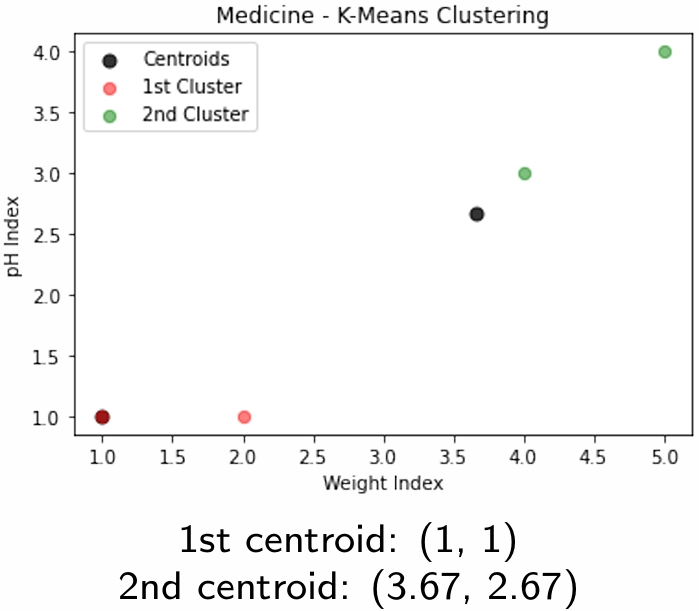
\includegraphics[scale=0.25]{chapter 5/ch5_figure15.jpeg}};
        \node (ch5_fig16) [rectangle, draw, right of=ch5_fig15]
        {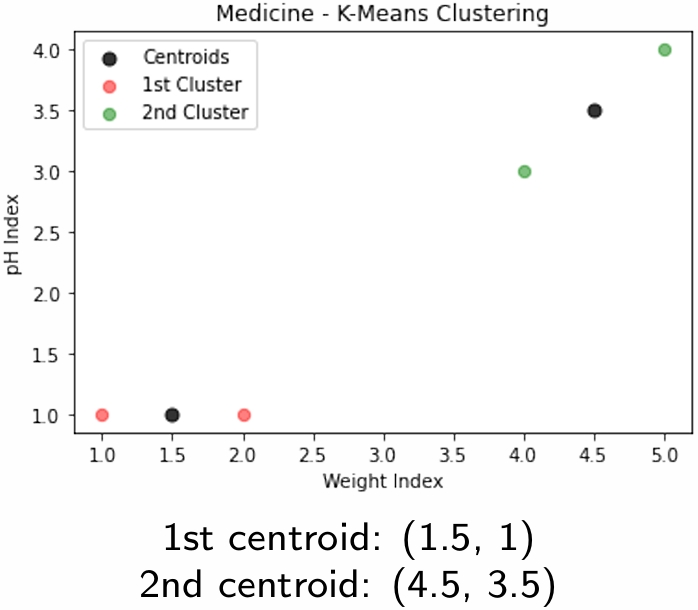
\includegraphics[scale=0.25]{chapter 5/ch5_figure16.jpeg}};
        \node (ch5_fig17) [rectangle, draw, right of=ch5_fig16]
        {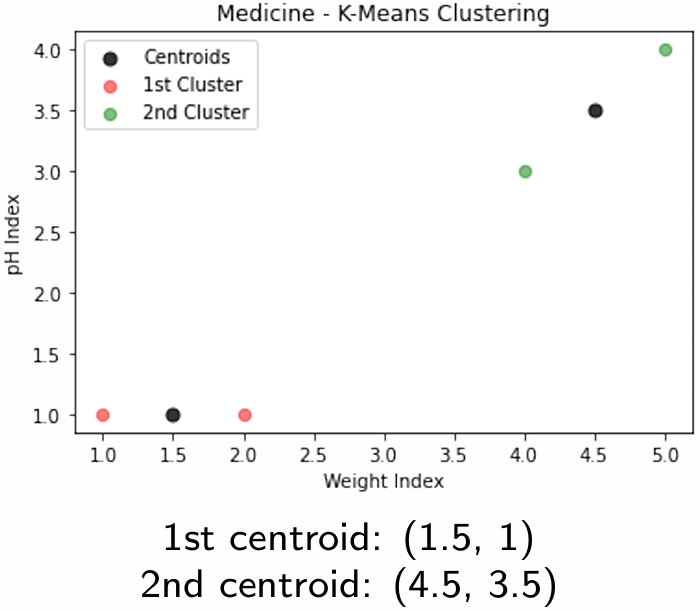
\includegraphics[scale=0.25]{chapter 5/ch5_figure17.jpeg}};

        \node[below of=ch5_fig15 , node distance=3.1cm] {First Iteration (1st Round)};
        \node[below of=ch5_fig16 , node distance=3.1cm] {Second Iteration (2nd Round)};
        \node[below of=ch5_fig17 , node distance=3.1cm] {Final Clusters (3rd Round)};

        \draw[->] (ch5_fig15) -- (ch5_fig16);
        \draw[->] (ch5_fig16) -- (ch5_fig17);
    \end{tikzpicture}
    \caption{Flowchart of the K-Means Clustering Algorithm}
    \label{ch5_fig15-17:flowchart_kmeans}
\end{figure}
\newpage
\textit{\large{K-Means Clustering Python Code Implementation using Scikit-Learn:}}\\
\begin{lstlisting}[language=Python, basicstyle=\ttfamily\small, keywordstyle=\color{blue}, commentstyle=\color{forestgreen}, stringstyle=\color{red}, showstringspaces=false]
# Import the required libraries
import numpy as np
from sklearn.cluster import KMeans
import matplotlib.pyplot as plt

# Create the training dataset
data = np.array([[1, 1], [2, 1], [4, 3], [5, 4]])

# Initial Centroids
init_centroids = np.array([[1, 1], [2, 1]])

# Create a KMeans object by specifying:
# - Number of clusters (n_clusters) = 2, Initial centroids (init) = init_centroids
# - Number of time the k-means algorithm will be run with different centroid seeds (n_init) = 1
# - Maximum number of iterations of the k-means algorithm for a single run (max_iter) = 3
kmeans = KMeans(n_clusters=2, init=init_centroids, n_init=1, max_iter=3)

kmeans.fit(data) # Compute k-means clustering
labels = kmeans.predict(data) # Predict the closest cluster each sample in data belongs to
centroids = kmeans.cluster_centers_ # Get resulting centroids of the clusters
fig, ax = plt.subplots() # Define 2D axes to plot 2D data into it

# Get boolean arrays representing entries with lables 0 and 1
a = np.array(labels == 0)
b = np.array(labels == 1)

# Plot centroids with color = black, size = 50 units, transparency = 20% and put label "Centroids"
ax.scatter(centroids[:, 0], centroids[:, 1], c='black', s=50, alpha=0.8, label="Centroids")

# Plot data in the different clusters (1st cluster = red, 2nd cluster = green) with transparency = 50%
ax.scatter(data[a, 0], data[a, 1], c="red", alpha=0.5, label="1st Cluster")
ax.scatter(data[b, 0], data[b, 1], c="green", alpha=0.5, label="2nd Cluster")
ax.legend() # Display the legend

ax.set_xlabel("Weight Index") # Set the x-axis label "Weight Index"
ax.set_ylabel("pH Index") # Set the y-axis label "pH Index"
ax.set_title("K-Means Clustering") # Set the title of the plot "K-Means Clustering"

# Output: Text(0.5, 1.0, 'Medicine - K-Means Clustering')
\end{lstlisting}
\begin{figure}[h]
    \centering
    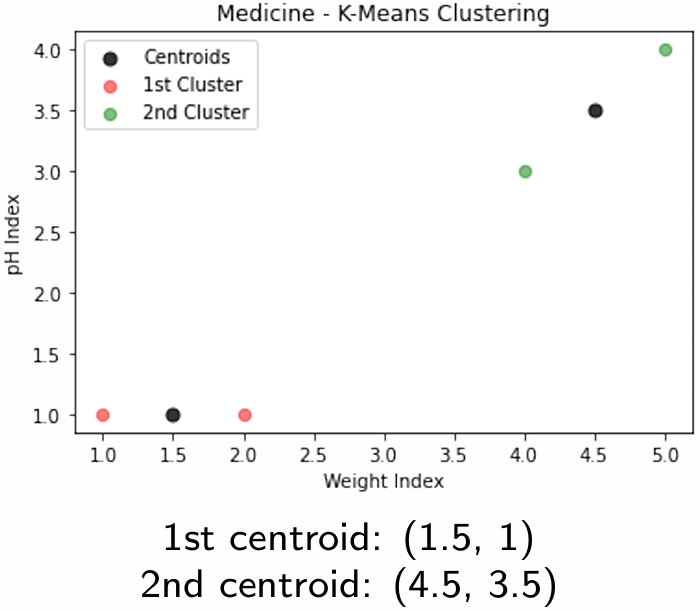
\includegraphics[scale=0.4]{chapter 5/ch5_figure17.jpeg}
    \caption{2D Plot of Medicines Clustered into 2 Groups using K-Means Clustering Algorithm}
\end{figure}

\chapter{Artificial Neural Network: Perceptron}
\textcolor{magenta}{\section{\textbf{Classification}}}
\begin{defBox}{Definition 6.1}{Classification}
    \raggedright
    \textcolor{cyan}{Classification} is the process of \textcolor{red}{predicting the class (labels/categories) of given data}.\\
    \begin{center}
        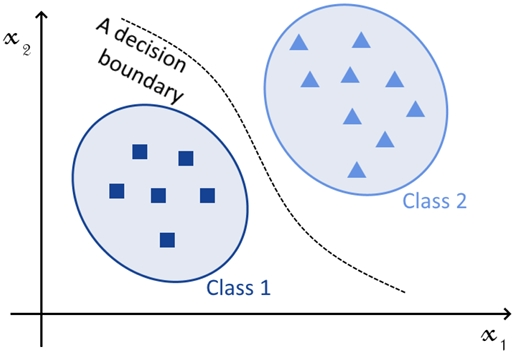
\includegraphics[scale=0.3]{chapter 6/ch6_figure1.jpeg}
    \end{center}
\end{defBox}
Examples of Classification:
\begin{enumerate}
    \item \textcolor{cyan}{Email Spam Detection}: Classify emails as 2 classes (\textcolor{violet}{Spam} or \textcolor{violet}{Not Spam}).
    \item \textcolor{cyan}{Images Classification \& Recognition}: Algorithm \& Subdomain of Computer Vision which \textcolor{violet}{looks at an image} and \textcolor{violet}{assigns it a label} from a collection of predicted labels/categories (e.g. dogs, cats, etc.).
    \begin{itemize}
        \item \textcolor{violet}{Vital components in robotics} like autonomous vehicles and domestic robots.
        \item Important in \textcolor{violet}{Security Systems} (e.g. Face Recognition), \textcolor{violet}{Image Search Engines} (e.g. Google Image Search) and \textcolor{violet}{Medical Imaging} (e.g. Cancer Detection).
    \end{itemize}
    \item \textcolor{cyan}{Handwritten Digit Recognition}: Classify handwritten digits as 10 classes (0-9).\\
    $\Rightarrow$ \textcolor{red}{Artificial Neural Networks} are used for this task to \textcolor{violet}{recognize/classify the handwritten digits}.
    \begin{figure}[h]
        \centering
        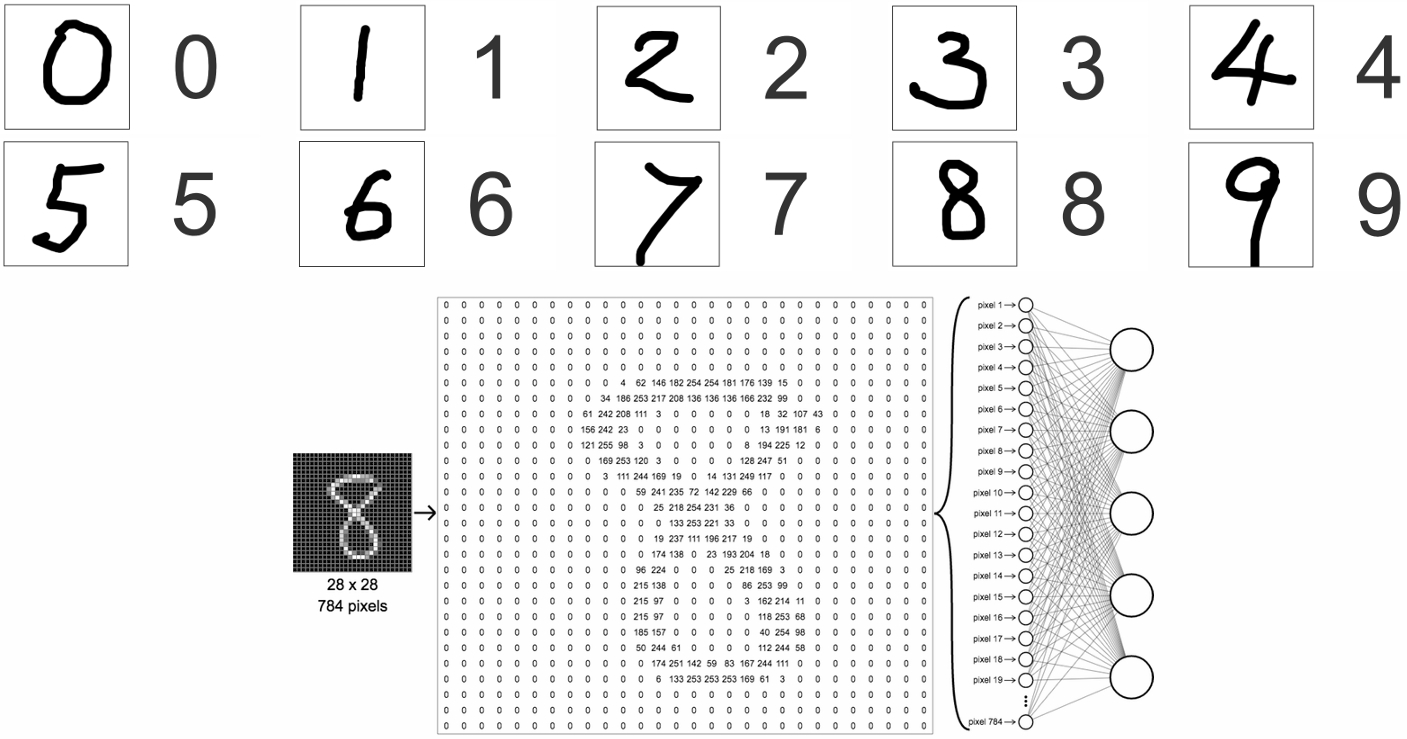
\includegraphics[scale=0.25]{chapter 6/ch6_figure2.jpeg}
        \caption{Handwritten Digit Recognition}
    \end{figure}
\end{enumerate}
\newpage
\textcolor{magenta}{\section{\textbf{Artificial Neural Network (ANN)}}}
\begin{defBox}{Definition 6.2}{Artificial Neural Network (ANN)}
    \raggedright
    \textcolor{cyan}{Artificial Neural Network (ANN)} considers a \textcolor{red}{universal function approximator} that transforms inputs into outputs.
    \begin{itemize}
    \item \textcolor{red}{Draws inspiration from neurons in our brain} and the way they are connected.
    \item One of the most popular and powerful artificial intelligence and machine learning algorithms.
    \end{itemize} 
    \begin{center}
        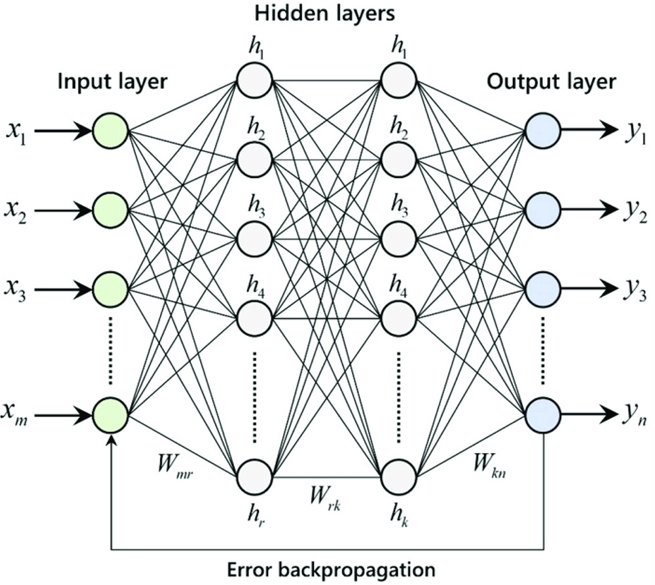
\includegraphics[scale=0.3]{chapter 6/ch6_figure3.jpeg}
    \end{center}
\end{defBox}
There are some differences in the structure between \textcolor{blue}{Biological Neurons} and \textcolor{blue}{Artificial Neurons}:
\begin{center}
    \begin{tabular}{|c|c|}
        \hline
        \rowcolor{lightblue}
        \textbf{Biological Neurons} & \textbf{Artificial Neurons}\\
        \hline
        Dendrites & Inputs Layer\\
        \hline
        Cell Nucleus (Computation Unit) & Node (Linear Function \& Activation Function)\\
        \hline
        Axon & Output Layer\\
        \hline
        Synapses & Weights\\
        \hline
    \end{tabular}
\end{center}
\begin{figure}[h]
    \centering
    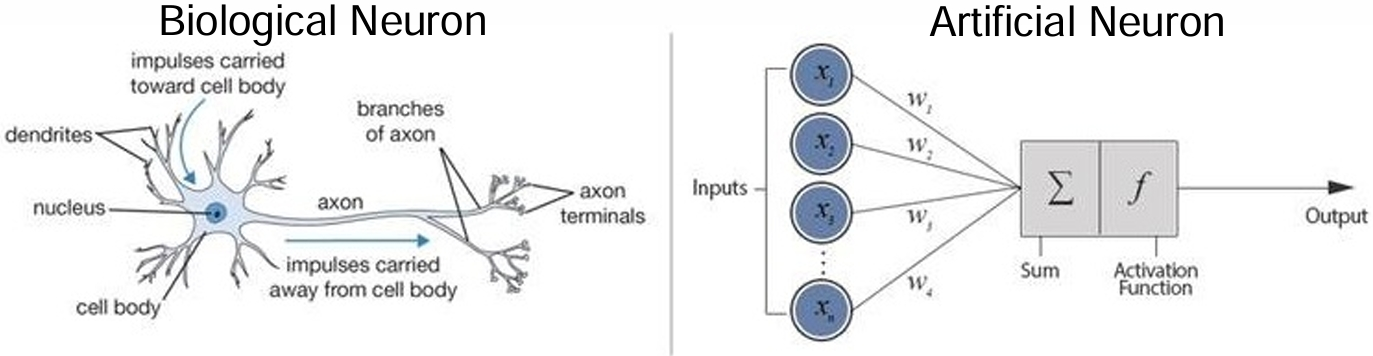
\includegraphics[scale=0.3]{chapter 6/ch6_figure4.jpeg}
    \caption{Biological Neurons vs. Artificial Neurons}
\end{figure}
\textcolor{magenta}{\section{\textbf{Introduction to Perceptron}}}
\begin{defBox}{Definition 6.3}{Perceptron}
    \raggedright
    \textcolor{cyan}{Perceptron} is \textcolor{cyan}{the simplest biological neuron model} in the ANN which performs certain \textcolor{red}{calculations to detect input data capabilities}.\\
    $\implies$ Name of an early algorithm for \textcolor{violet}{supervised learning} of \textcolor{violet}{binary classifiers} with only two classes.
    \begin{center}
        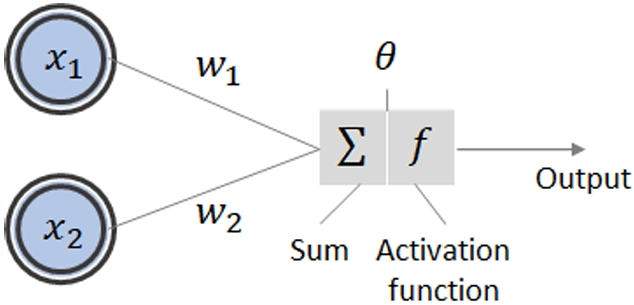
\includegraphics[scale=0.3]{chapter 6/ch6_figure5.jpeg}
    \end{center}
\end{defBox}
Perceptron was invented in 1957 by \textcolor{violet}{Frank Rosenblatt}, described as the first machine "capable of having an original idea".
\newpage
\begin{egBox}{Example 6.3}{Perceptron}
    \raggedright
    Assume we have \(\text{output} = f(w_1 \times x_1 + w_2 \times x_2 + \theta)\) where:\\
    \begin{itemize}
        \item \(x_1\) and \(x_2\) are the input signals.
        \item \(w_1\) and \(w_2\) are the weights.
        \item \(\theta\) is the bias.
        \item \(f\) is the activation function.
    \end{itemize}
    \vspace{3mm}
    Suppose \(x_1 = 3\), \(x_2 = 5\), \(w_1 = 0.2\), \(w_2 = 0.3\), \(\theta = 0.3\) and \(f(x) = \frac{1}{1+e^{-x}}\):
    \[
        \text{output} = f(0.2 \times 3 + 0.3 \times 5 + 0.3) = f(2.4) = \frac{1}{1+e^{-2.4}} = \underline{\underline{0.91683}}
    \]
\end{egBox}
\textcolor{magenta}{\section{\textbf{Perceptron Learning Rules}}}
\begin{thmBox}{Theorem 6.4}{Perceptron Learning Rules}
    \raggedright
    Rules that \textcolor{purple}{the output of the perceptron for the new weights is closer to \(T\)}.\\
    For \(i \in {1, 2}\):
    \[
        \triangle w_i = \eta(T - O)x_i
    \]
    \[
        \triangle \theta = \eta(T - O)
    \]
    \[
        \text{New Weight } w_i = \text{Old Weight } w_i + \triangle w_i
    \]
    \[
        \text{New Bias } \theta = \text{Old Bias } \theta + \triangle \theta
    \]
    where:\\
    \begin{itemize}
        \item \(\textcolor{brown}{x_1}\) \& \(\textcolor{brown}{x_2}\): Inputs.
        \item \(\textcolor{brown}{\theta}\): Bias.
        \item \(\textcolor{brown}{w_1}\) \& \(\textcolor{brown}{w_2}\): Weights.
        \item \(\textcolor{brown}{O}\): Computed Output.
        \item \(\textcolor{brown}{T}\): Target Output.
        \item \(\textcolor{brown}{\triangle w_1}\): Change in Weight 1 \(w_1\).
        \item \(\textcolor{brown}{\triangle w_2}\): Change in Weight 2 \(w_2\).
        \item \(\textcolor{brown}{\triangle \theta}\): Change in Bias \(\theta\).
        \item \(\textcolor{brown}{\eta}\): Learning Rate.
    \end{itemize}
\end{thmBox}
The Perceptron Learning Rules are used to adjust the weights and the bias to minimize the error in the output.\\\
There are 2 cases in the Perceptron Learning Rules:
\begin{enumerate}
    \item If the \textcolor{cyan}{output is correct (\(T = O\))}, the weights \textcolor{red}{\(w_1 \text{ and } w_2\) are not updated}.
    \item If the \textcolor{cyan}{output is incorrect (\(T \neq O\))}, the weights \textcolor{red}{\(w_1 \text{ and } w_2\) are updated} to minimize the error.
\end{enumerate}
\vspace{2mm}
\underline{Example of Perceptron Learning Rules: Logical AND}\\
Suppose we will work on a problem of AND logical operation.\\
Assume the weights and bias are initialized as \(w_1 = 0.1\), \(w_2 = 0.5\) and \(\theta = -0.8\). Also, the learning rate is \(\eta = 0.2\).\\
Activation Function is:
\[
    f(x) = \begin{cases}
        0 & \text{if } x \leq 0\\
        1 & \text{otherwise}
    \end{cases}
\]
The truth table of logical AND is:\\
\begin{figure}[ht]
    \raggedright
    \begin{tikzpicture}[node distance=9.5cm]
        \node (ch6_fig6)
        {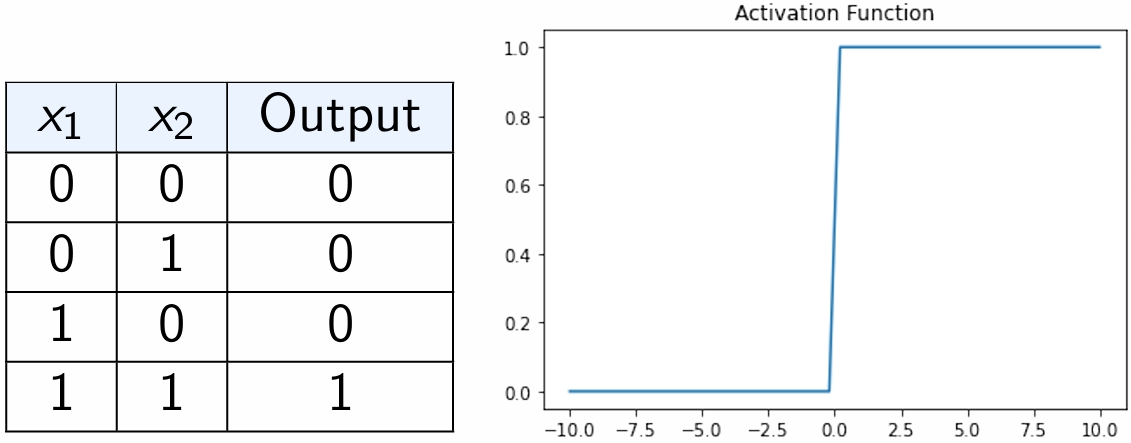
\includegraphics[scale=0.25]{chapter 6/ch6_figure6.jpeg}};
        \node (ch6_fig7) [right of=ch6_fig6]
        {\includegraphics[scale=0.25]{chapter 6/ch6_figure7.jpeg}};
    \end{tikzpicture}
\end{figure}
{\scriptsize (Note: The \textcolor{yellow}{yellow highlighted rows} in the tables below are the incorrect outputs.)}
\newpage
\uwave{Initial Round}\\
\begin{center}
    \begin{tabular}{|c|c|c|c|c|c|c|c|c|c|}
        \hline
        \rowcolor{lightblue}
        \textbf{\(x_1\)} & \textbf{\(x_2\)} & \textbf{\(T\)} & \textbf{\(O\)} & \textbf{\(\triangle w_1\)} & \textbf{\(w_1\)} & \textbf{\(\triangle w_2\)} & \textbf{\(w_2\)} & \textbf{\(\triangle \theta\)} & \textbf{\(\theta\)}\\
        \hline
        \textcolor{red}{-} & \textcolor{red}{-} & \textcolor{red}{-} & \textcolor{red}{-} & \textcolor{red}{-} & \textcolor{red}{0.1} & \textcolor{red}{-} & \textcolor{red}{0.5} & \textcolor{red}{-} & \textcolor{red}{-0.8}\\      \hline
        & & & & & & & & & \\
        \hline
        & & & & & & & & & \\
        \hline
        & & & & & & & & & \\
        \hline
        & & & & & & & & & \\
        \hline
        & & & & & & & & & \\
        \hline
        & & & & & & & & & \\
        \hline
        & & & & & & & & & \\
        \hline
        & & & & & & & & & \\
        \hline
        & & & & & & & & & \\
        \hline
        & & & & & & & & & \\
        \hline
        & & & & & & & & & \\
        \hline
        & & & & & & & & & \\
        \hline
        & & & & & & & & & \\
        \hline
        & & & & & & & & & \\
        \hline
        & & & & & & & & & \\
        \hline
        & & & & & & & & & \\
        \hline
    \end{tabular}
\end{center}
\vspace{1cm}
\uwave{Round 1}\\
\begin{center}
    \begin{tabular}{|c|c|c|c|c|c|c|c|c|c|c|c }
        \cline{1-10}
        \rowcolor{lightblue}
        \textbf{\(x_1\)} & \textbf{\(x_2\)} & \textbf{\(T\)} & \textbf{\(O\)} & \textbf{\(\triangle w_1\)} & \textbf{\(w_1\)} & \textbf{\(\triangle w_2\)} & \textbf{\(w_2\)} & \textbf{\(\triangle \theta\)} & \textbf{\(\theta\)} & \cellcolor{white}{}\\
        \cline{1-10}
        - & - & - & - & - & 0.1 & - & 0.5 & - & -0.8 & \\
        \cline{1-10}
        \textcolor{red}{0} & \textcolor{red}{0} & \textcolor{red}{0} & \textcolor{red}{0} & \textcolor{red}{0} & \textcolor{red}{0.1} & \textcolor{red}{0} & \textcolor{red}{0.5} & \textcolor{red}{0} & \textcolor{red}{-0.8} & \textcolor{blue}{\textbf{Step 1}}\\
        \cline{1-10}
        \textcolor{red}{0} & \textcolor{red}{1} & \textcolor{red}{0} & \textcolor{red}{0} & \textcolor{red}{0} & \textcolor{red}{0.1} & \textcolor{red}{0} & \textcolor{red}{0.5} & \textcolor{red}{0} & \textcolor{red}{-0.8} & \textcolor{blue}{\textbf{Step 2}} \\
        \cline{1-10}
        \textcolor{red}{1} & \textcolor{red}{0} & \textcolor{red}{0} & \textcolor{red}{0} & \textcolor{red}{0} & \textcolor{red}{0.1} & \textcolor{red}{0} & \textcolor{red}{0.5} & \textcolor{red}{0} & \textcolor{red}{-0.8} & \textcolor{blue}{\textbf{Step 3}} \\
        \cline{1-10}
        \rowcolor{lightyellow}
        \textcolor{red}{1} & \textcolor{red}{1} & \textcolor{red}{1} & \textcolor{red}{0} & \textcolor{red}{0.2} & \textcolor{red}{0.3} & \textcolor{red}{0.2} & \textcolor{red}{0.7} & \textcolor{red}{0.2} & \textcolor{red}{-0.6} & \cellcolor{white}{\textcolor{blue}{\textbf{Step 4}}}\\
        \cline{1-10}
        & & & & & & & & & & \\
        \cline{1-10}
        & & & & & & & & & & \\
        \cline{1-10}
        & & & & & & & & & & \\
        \cline{1-10}
        & & & & & & & & & & \\
        \cline{1-10}
        & & & & & & & & & & \\
        \cline{1-10}
        & & & & & & & & & & \\
        \cline{1-10}
        & & & & & & & & & & \\
        \cline{1-10}
        & & & & & & & & & & \\
        \cline{1-10}
        & & & & & & & & & & \\
        \cline{1-10}
        & & & & & & & & & & \\
        \cline{1-10}
        & & & & & & & & & & \\
        \cline{1-10}
        & & & & & & & & & & \\
        \cline{1-10}
    \end{tabular}
\end{center}
\vspace{1cm}
\uwave{Round 2}\\
\begin{center}
    \begin{tabular}{|c|c|c|c|c|c|c|c|c|c|c|c }
        \cline{1-10}
        \rowcolor{lightblue}
        \textbf{\(x_1\)} & \textbf{\(x_2\)} & \textbf{\(T\)} & \textbf{\(O\)} & \textbf{\(\triangle w_1\)} & \textbf{\(w_1\)} & \textbf{\(\triangle w_2\)} & \textbf{\(w_2\)} & \textbf{\(\triangle \theta\)} & \textbf{\(\theta\)} & \cellcolor{white}{}\\
        \cline{1-10}
        - & - & - & - & - & 0.1 & - & 0.5 & - & -0.8 & \\
        \cline{1-10}
        0 & 0 & 0 & 0 & 0 & 0.1 & 0 & 0.5 & 0 & -0.8 & \\
        \cline{1-10}
        0 & 1 & 0 & 0 & 0 & 0.1 & 0 & 0.5 & 0 & -0.8 & \\
        \cline{1-10}
        1 & 0 & 0 & 0 & 0 & 0.1 & 0 & 0.5 & 0 & -0.8 & \\
        \cline{1-10}
        \rowcolor{lightyellow}
        1 & 1 & 1 & 0 & 0.2 & 0.3 & 0.2 & 0.7 & 0.2 & -0.6 & \cellcolor{white}{} \\
        \cline{1-10}
        \textcolor{red}{0} & \textcolor{red}{0} & \textcolor{red}{0} & \textcolor{red}{0} & \textcolor{red}{0} & \textcolor{red}{0.3} & \textcolor{red}{0} & \textcolor{red}{0.7} & \textcolor{red}{0} & \textcolor{red}{-0.6} & \textcolor{blue}{\textbf{Step 1}}\\
        \cline{1-10}
        \rowcolor{lightyellow}
        \textcolor{red}{0} & \textcolor{red}{1} & \textcolor{red}{0} & \textcolor{red}{1} & \textcolor{red}{0} & \textcolor{red}{0.3} & \textcolor{red}{-0.2} & \textcolor{red}{0.5} & \textcolor{red}{-0.2} & \textcolor{red}{-0.8} & \cellcolor{white}{\textcolor{blue}{\textbf{Step 2}}} \\
        \cline{1-10}
        \textcolor{red}{1} & \textcolor{red}{0} & \textcolor{red}{0} & \textcolor{red}{0} & \textcolor{red}{0} & \textcolor{red}{0.3} & \textcolor{red}{0} & \textcolor{red}{0.5} & \textcolor{red}{0} & \textcolor{red}{-0.8} & \textcolor{blue}{\textbf{Step 3}} \\
        \cline{1-10}
        \rowcolor{lightyellow}
        \textcolor{red}{1} & \textcolor{red}{1} & \textcolor{red}{1} & \textcolor{red}{0} & \textcolor{red}{0.2} & \textcolor{red}{0.5} & \textcolor{red}{0.2} & \textcolor{red}{0.7} & \textcolor{red}{0.2} & \textcolor{red}{-0.6} & \cellcolor{white}{\textcolor{blue}{\textbf{Step 4}}}\\
        \cline{1-10}
        & & & & & & & & & & \\
        \cline{1-10}
        & & & & & & & & & & \\
        \cline{1-10}
        & & & & & & & & & & \\
        \cline{1-10}
        & & & & & & & & & & \\
        \cline{1-10}
        & & & & & & & & & & \\
        \cline{1-10}
        & & & & & & & & & & \\
        \cline{1-10}
        & & & & & & & & & & \\
        \cline{1-10}
        & & & & & & & & & & \\
        \cline{1-10}
    \end{tabular}
\end{center}
\newpage
\uwave{Round 3}\\
\begin{center}
    \begin{tabular}{|c|c|c|c|c|c|c|c|c|c|c|c }
        \cline{1-10}
        \rowcolor{lightblue}
        \textbf{\(x_1\)} & \textbf{\(x_2\)} & \textbf{\(T\)} & \textbf{\(O\)} & \textbf{\(\triangle w_1\)} & \textbf{\(w_1\)} & \textbf{\(\triangle w_2\)} & \textbf{\(w_2\)} & \textbf{\(\triangle \theta\)} & \textbf{\(\theta\)} & \cellcolor{white}{}\\
        \cline{1-10}
        - & - & - & - & - & 0.1 & - & 0.5 & - & -0.8 & \\
        \cline{1-10}
        0 & 0 & 0 & 0 & 0 & 0.1 & 0 & 0.5 & 0 & -0.8 & \\
        \cline{1-10}
        0 & 1 & 0 & 0 & 0 & 0.1 & 0 & 0.5 & 0 & -0.8 & \\
        \cline{1-10}
        1 & 0 & 0 & 0 & 0 & 0.1 & 0 & 0.5 & 0 & -0.8 & \\
        \cline{1-10}
        \rowcolor{lightyellow}
        1 & 1 & 1 & 0 & 0.2 & 0.3 & 0.2 & 0.7 & 0.2 & -0.6 & \cellcolor{white}{} \\
        \cline{1-10}
        0 & 0 & 0 & 0 & 0 & 0.3 & 0 & 0.7 & 0 & -0.6 & \\
        \cline{1-10}
        \rowcolor{lightyellow}
        0 & 1 & 0 & 1 & 0 & 0.3 & -0.2 & 0.5 & -0.2 & -0.8 & \cellcolor{white}{} \\
        \cline{1-10}
        1 & 0 & 0 & 0 & 0 & 0.3 & 0 & 0.5 & 0 & -0.8 & \\
        \cline{1-10}
        \rowcolor{lightyellow}
        1 & 1 & 1 & 0 & 0.2 & 0.5 & 0.2 & 0.7 & 0.2 & -0.6 & \cellcolor{white}{}\\
        \cline{1-10}
        \textcolor{red}{0} & \textcolor{red}{0} & \textcolor{red}{0} & \textcolor{red}{0} & \textcolor{red}{0} & \textcolor{red}{0.5} & \textcolor{red}{0} & \textcolor{red}{0.7} & \textcolor{red}{0} & \textcolor{red}{-0.6} & \textcolor{blue}{\textbf{Step 1}}\\
        \cline{1-10}
        \rowcolor{lightyellow}
        \textcolor{red}{0} & \textcolor{red}{1} & \textcolor{red}{0} & \textcolor{red}{1} & \textcolor{red}{0} & \textcolor{red}{0.5} & \textcolor{red}{-0.2} & \textcolor{red}{0.5} & \textcolor{red}{-0.2} & \textcolor{red}{-0.8} & \cellcolor{white}{\textcolor{blue}{\textbf{Step 2}}} \\
        \cline{1-10}
        \textcolor{red}{1} & \textcolor{red}{0} & \textcolor{red}{0} & \textcolor{red}{0} & \textcolor{red}{0} & \textcolor{red}{0.5} & \textcolor{red}{0} & \textcolor{red}{0.5} & \textcolor{red}{0} & \textcolor{red}{-0.8} & \textcolor{blue}{\textbf{Step 3}} \\
        \cline{1-10}
        \textcolor{red}{1} & \textcolor{red}{1} & \textcolor{red}{1} & \textcolor{red}{1} & \textcolor{red}{0} & \textcolor{red}{0.5} & \textcolor{red}{0} & \textcolor{red}{0.5} & \textcolor{red}{0} & \textcolor{red}{-0.8} & \textcolor{blue}{\textbf{Step 4}}\\
        \cline{1-10}
        & & & & & & & & & & \\
        \cline{1-10}
        & & & & & & & & & & \\
        \cline{1-10}
        & & & & & & & & & & \\
        \cline{1-10}
        & & & & & & & & & & \\
        \cline{1-10}
    \end{tabular}
\end{center}
\vspace{1cm}
\uwave{Round 4}\\
\begin{center}
    \begin{tabular}{|c|c|c|c|c|c|c|c|c|c|c|c }
        \cline{1-10}
        \rowcolor{lightblue}
        \textbf{\(x_1\)} & \textbf{\(x_2\)} & \textbf{\(T\)} & \textbf{\(O\)} & \textbf{\(\triangle w_1\)} & \textbf{\(w_1\)} & \textbf{\(\triangle w_2\)} & \textbf{\(w_2\)} & \textbf{\(\triangle \theta\)} & \textbf{\(\theta\)} & \cellcolor{white}{}\\
        \cline{1-10}
        - & - & - & - & - & 0.1 & - & 0.5 & - & -0.8 & \\
        \cline{1-10}
        0 & 0 & 0 & 0 & 0 & 0.1 & 0 & 0.5 & 0 & -0.8 & \\
        \cline{1-10}
        0 & 1 & 0 & 0 & 0 & 0.1 & 0 & 0.5 & 0 & -0.8 & \\
        \cline{1-10}
        1 & 0 & 0 & 0 & 0 & 0.1 & 0 & 0.5 & 0 & -0.8 & \\
        \cline{1-10}
        \rowcolor{lightyellow}
        1 & 1 & 1 & 0 & 0.2 & 0.3 & 0.2 & 0.7 & 0.2 & -0.6 & \cellcolor{white}{} \\
        \cline{1-10}
        0 & 0 & 0 & 0 & 0 & 0.3 & 0 & 0.7 & 0 & -0.6 & \\
        \cline{1-10}
        \rowcolor{lightyellow}
        0 & 1 & 0 & 1 & 0 & 0.3 & -0.2 & 0.5 & -0.2 & -0.8 & \cellcolor{white}{} \\
        \cline{1-10}
        1 & 0 & 0 & 0 & 0 & 0.3 & 0 & 0.5 & 0 & -0.8 & \\
        \cline{1-10}
        \rowcolor{lightyellow}
        1 & 1 & 1 & 0 & 0.2 & 0.5 & 0.2 & 0.7 & 0.2 & -0.6 & \cellcolor{white}{}\\
        \cline{1-10}
        0 & 0 & 0 & 0 & 0 & 0.5 & 0 & 0.7 & 0 & -0.6 & \\
        \cline{1-10}
        \rowcolor{lightyellow}
        0 & 1 & 0 & 1 & 0 & 0.5 & -0.2 & 0.5 & -0.2 & -0.8 & \cellcolor{white}{} \\
        \cline{1-10}
        1 & 0 & 0 & 0 & 0 & 0.5 & 0 & 0.5 & 0 & -0.8 & \\
        \cline{1-10}
        1 & 1 & 1 & 1 & 0 & 0.5 & 0 & 0.5 & 0 & -0.8 & \\
        \cline{1-10}
        \textcolor{red}{0} & \textcolor{red}{0} & \textcolor{red}{0} & \textcolor{red}{0} & \textcolor{red}{0} & \textcolor{red}{0.5} & \textcolor{red}{0} & \textcolor{red}{0.5} & \textcolor{red}{0} & \textcolor{red}{-0.8} & \textcolor{blue}{\textbf{Step 1}}\\
        \cline{1-10}
        \textcolor{red}{0} & \textcolor{red}{1} & \textcolor{red}{0} & \textcolor{red}{0} & \textcolor{red}{0} & \textcolor{red}{0.5} & \textcolor{red}{0} & \textcolor{red}{0.5} & \textcolor{red}{0} & \textcolor{red}{-0.8} & \textcolor{blue}{\textbf{Step 2}} \\
        \cline{1-10}
        \textcolor{red}{1} & \textcolor{red}{0} & \textcolor{red}{0} & \textcolor{red}{0} & \textcolor{red}{0} & \textcolor{red}{0.5} & \textcolor{red}{0} & \textcolor{red}{0.5} & \textcolor{red}{0} & \textcolor{red}{-0.8} & \textcolor{blue}{\textbf{Step 3}} \\
        \cline{1-10}
        \textcolor{red}{1} & \textcolor{red}{1} & \textcolor{red}{1} & \textcolor{red}{1} & \textcolor{red}{0} & \textcolor{red}{0.5} & \textcolor{red}{0} & \textcolor{red}{0.5} & \textcolor{red}{0} & \textcolor{red}{-0.8} & \textcolor{blue}{\textbf{Step 4}}\\
        \cline{1-10}
    \end{tabular}
\end{center}
\vspace{1cm}
\uwave{Final Result}\\
\begin{center}
    \begin{tabular}{|c|c|c|c|c|c|c|c|c|c|c|}
        \hline
        \rowcolor{lightblue}
        \textbf{\(x_1\)} & \textbf{\(x_2\)} & \textbf{\(T\)} & \textbf{\(O\)} & \textbf{\(\triangle w_1\)} & \textbf{\(w_1\)} & \textbf{\(\triangle w_2\)} & \textbf{\(w_2\)} & \textbf{\(\triangle \theta\)} & \textbf{\(\theta\)}\\
        \hline
        - & - & - & - & - & 0.1 & - & 0.5 & - & -0.8\\
        \hline
        0 & 0 & 0 & 0 & 0 & 0.1 & 0 & 0.5 & 0 & -0.8\\
        \hline
        0 & 1 & 0 & 0 & 0 & 0.1 & 0 & 0.5 & 0 & -0.8\\
        \hline
        1 & 0 & 0 & 0 & 0 & 0.1 & 0 & 0.5 & 0 & -0.8\\
        \hline
        \rowcolor{lightyellow}
        1 & 1 & 1 & 0 & 0.2 & 0.3 & 0.2 & 0.7 & 0.2 & -0.6\\
        \hline
        0 & 0 & 0 & 0 & 0 & 0.3 & 0 & 0.7 & 0 & -0.6\\
        \hline
        \rowcolor{lightyellow}
        0 & 1 & 0 & 1 & 0 & 0.3 & -0.2 & 0.5 & -0.2 & -0.8\\
        \hline
        1 & 0 & 0 & 0 & 0 & 0.3 & 0 & 0.5 & 0 & -0.8\\
        \hline
        \rowcolor{lightyellow}
        1 & 1 & 1 & 0 & 0.2 & 0.5 & 0.2 & 0.7 & 0.2 & -0.6\\
        \hline
        0 & 0 & 0 & 0 & 0 & 0.5 & 0 & 0.7 & 0 & -0.6\\
        \hline
        \rowcolor{lightyellow}
        0 & 1 & 0 & 1 & 0 & 0.5 & -0.2 & 0.5 & -0.2 & -0.8\\
        \hline
        1 & 0 & 0 & 0 & 0 & 0.5 & 0 & 0.5 & 0 & -0.8\\
        \hline
        1 & 1 & 1 & 1 & 0 & 0.5 & 0 & 0.5 & 0 & -0.8\\
        \hline
        0 & 0 & 0 & 0 & 0 & 0.5 & 0 & 0.5 & 0 & -0.8\\
        \hline
        0 & 1 & 0 & 0 & 0 & 0.5 & 0 & 0.5 & 0 & -0.8\\
        \hline
        1 & 0 & 0 & 0 & 0 & 0.5 & 0 & 0.5 & 0 & -0.8\\
        \hline
        1 & 1 & 1 & 1 & 0 & 0.5 & 0 & 0.5 & 0 & -0.8\\
        \hline
    \end{tabular}
\end{center}
\textcolor{blue}{We can stop the training process since all the outputs are correct, actually we can stop it after we test $x_1 = 0$ and $x_2 = 1$.}\\
$\because$ The training converges in \textcolor{red}{4 epoches} if the initial weights and bias are \(w_1 = 0.1\), \(w_2 = 0.5\) and \(\theta = -0.8\) with a learning rate of \(\eta = 0.2\).\\
$\therefore$ The final weights and bias are \(\underline{\underline{w_1 = 0.5}}\), \(\underline{\underline{w_2 = 0.5}}\) and \(\underline{\underline{\theta = -0.8}}\).
\newpage
\textit{\large{Perceptron Python Code implementation from Scratch:}}
\begin{lstlisting}[language=Python, basicstyle=\ttfamily\small, keywordstyle=\color{blue}, commentstyle=\color{forestgreen}, stringstyle=\color{red}, showstringspaces=false] 
import math                         # Import math module

class Perceptron:
    def __init__(self):
        """ Perceptron Initialization """
        self.w = [0.1, 0.5]         # Weights
        self.theta = -0.8           # Bias
        self.learningRate = 0.2     # Eta 
    
    def response(self, x):
        """ Perceptron Response """
        # Calculate the Weighted Sum
        y = x[0] * self.w[0] + x[1] * self.w[1] + self.theta
        # If the Weighted Sum is greater than 0, return 1, otherwise return 0
        if y > 0:
            return 1
        else:
            return 0

    def updateWeights(self, x, iterError):
        """ Weights Update """
        # w_i = w_i + eta * (T - O) * x_i
        self.w[0] += self.learningRate * iterError * x[0]
        self.w[1] += self.learningRate * iterError * x[1]

    def updateBias(self, iterError):
        """ Bias Update """
        # theta = theta + eta * (T - O)
        self.theta += self.learningRate * iterError

    def train(self, data):
        """ Perceptron Training """
        learned = True      # Should Perform Training
        round = 0           # Initialize round to 0
    
        while learned:                                  # While learned is true
            totalError = 0.0                            # Initialize totalError to 0
            for x in data:                              # For each data in the dataset
                r = self.response(x)                    # Calculate perceptron output of X
                if x[2] != r:                           # If the output is different from the target
                    roundError = x[2] - r               # Round Error = Target- Perceptron Output
                    self.updateWeights(x, roundError)   # Update Weights
                    self.updateBias(roundError)         # Update Bias
                    totalError += abs(roundError)       # Update Total Error
            round += 1                                  # Increment Round
            
            # Don't use == since floating point numbers are not exact
            if math.isclose(totalError, 0) or round >= 100:       # Stopping Condition
                print("Total Number of Rounds (Epochs): ", round) # Print the total number of rounds
                print("Final Weights: ", self.w)                  # Print the final weights
                print("Final Bias: ", self.theta)                 # Print the final bias
                learned = False                                   # Stop Learning

""" Main Function """
perceptron = Perceptron()                                   # Create Perceptron Object
trainset = [[0, 0, 0], [0, 1, 0], [1, 0, 0], [1, 1, 1]]     # Define Training Dataset
perceptron.train(trainset)                                  # Train the Perceptron



# Output:

# Total Number of Rounds (Epochs):  4
# Final Weights:  [0.5, 0.49999999999999994]
# Final Bias:  -0.8
\end{lstlisting}
\newpage
\textit{\large{Perceptron Python Code Implementation using Scikit-Learn:}}
\begin{lstlisting}[language=Python, basicstyle=\ttfamily\small, keywordstyle=\color{blue}, commentstyle=\color{forestgreen}, stringstyle=\color{red}, showstringspaces=false]
import numpy as np                              # Import NumPy
from sklearn.linear_model import Perceptron     # Import Perceptron class from Scikit-Learn

# Define the Training Dataset
inputs = np.array([[0, 0], [0, 1], [1, 0], [1, 1]])     # Inputs
outputs = np.array([0, 0, 0, 1])                        # Expected Outputs

# Create and Fit the Perceptron Model
# Set Learning Rate to 0.2 (eta0 = 0.2)
model = Perceptron(eta0=0.2)
model.fit(inputs, outputs)

# Use the trained model to predict the Outputs
predicted_outputs = model.predict([[0, 0], [1, 0], [1, 1], [0, 1]])
print("Predicted Outputs: ", predicted_outputs)     # Print the Predicted Outputs

print("Weights: ", model.coef_)                     # Print the Final Weights
print("Bias: ", model.intercept_)                   # Print the Final Bias



# Output:

# Predicted Outputs:  [0 0 1 0]
# Weights:  [[0.4 0.2]]
# Bias:  [-0.4]
\end{lstlisting}
\textcolor{magenta}{\section{\textbf{Perceptron Stopping Rules}}}
\begin{itemize}
    \item \textcolor{cyan}{Use Maximum Training Time}: The training may go a bit beyond the specified time limit to complete the current epoch.
    \item \textcolor{cyan}{Maximum Number of Training Cycles Allowed}: If the maximum number of cycles is exceeded, then training stops.
    \item \textcolor{cyan}{Use Minimum Accuracy}: Training will continue until the specified accuracy is attained.
\end{itemize}
\textcolor{magenta}{\section{\textbf{Perceptron Learning and Epoch Terminologies}}}
\begin{defBox}{Definition 6.6.1}{Learning}
    \textcolor{cyan}{Learning} is the \textcolor{red}{process of updating weights and bias} in a perceptron to minimize the error between the predicted and actual outputs.
\end{defBox}
\begin{defBox}{Definition 6.6.2}{Epoch}
    \textcolor{cyan}{Epoch} is a \textcolor{red}{single cycle through the full training dataset} during the training process.
\end{defBox}
\newpage
\begin{egBox}{Example 6.6}{Learning and Epoch}
    \raggedright
    The initial weights are set to \(w_1 = 0.1\) and \(w_2 = 0.5\) but it causes some errors.\\
    The whole learning process takes 4 rounds/epoches to coneverge and update the weight values to 0.5 and predict all the outputs correctly.\\
    By the final results of the perceptron learning procedure, the final weights are \(w_1 = 0.5\) and \(w_2 = 0.5\).\\
    \vspace{3mm}
    The relationship between the inputs \(x_1\) and \(x_2\) and the output \(y\) is given by the equation:
    \[
        y = \begin{cases}
            0 & \text{if } 0.5x_1 + 0.5x_2 - 0.8 \leq 0\\
            1 & \text{otherwise}
        \end{cases} = \begin{cases}
            0 & \text{if } x_1 + x_2 \leq 1.6\\
            1 & \text{otherwise}
        \end{cases}
    \]
    The decision boundary shown in the figure below separates the two classes of points.\\
    \begin{center}
        \includegraphics[scale=0.3]{chapter 6/ch6_figure8.jpeg}
    \end{center}
\end{egBox}
\fbox{
    \parbox{0.97\textwidth}{
        \textbf{Remark:}\\
        If we run another sets of weights and bias, it will take more or less rounds to converge.\\
        The equation of line may be different but the decision boundary will be the same.\\
        $\implies$ \textcolor{red}{The decision boundary is the same for all the perceptron models.}
    }
}\\


\textcolor{magenta}{\section{\textbf{Perceptron Limiitations}}}
There are some limitations of the perceptron model:
\begin{enumerate}
    \item Can only represent a \textcolor{cyan}{limited set of functions}.
    \item Can only distinguish the sets of inputs that are \textcolor{cyan}{linearly separable in the inputs} by the values of its output.\\
    (e.g. Cannot solve the XOR problem)
\end{enumerate}
\vspace{3mm}
To remedy these limitation, the \textcolor{red}{Multi-Layer Perceptron (MLP)} model is used.


\newpage
\textbf{\textcolor{purple}{\Large{Practice Problem}}}\\
\textbf{Question}:\\
Please apply the perceptron learning procedure for the OR gate. The truth table for the logical OR is given below:\\
\vspace{2mm}
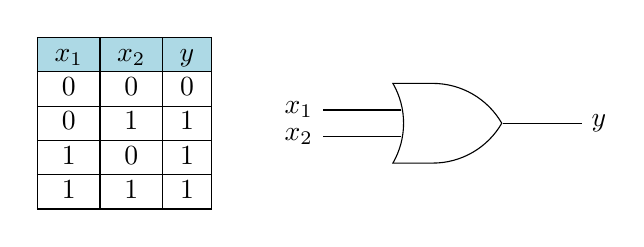
\begin{tikzpicture}
    
    \begin{scope}[shift={(0,0)}]
        \node at (0,0) {
            \begin{tabular}{|c|c|c|}
            \hline
            \rowcolor{lightblue}
            \textbf{\(x_1\)} & \textbf{\(x_2\)} & \textbf{\(y\)}\\
            \hline
            0 & 0 & 0\\
            \hline
            0 & 1 & 1\\
            \hline
            1 & 0 & 1\\
            \hline
            1 & 1 & 1\\
            \hline
            \end{tabular}
        };
        \end{scope}
        \node [or gate US, draw, rotate=0, logic gate inputs=nn, scale=2] at (4,0) (OR) {};
        \draw (OR.input 1) -- ++(-1,0) node[left] {\(x_1\)};
        \draw (OR.input 2) -- ++(-1,0) node[left] {\(x_2\)};
        \draw (OR.output) -- ++(1,0) node[right] {\(y\)};
\end{tikzpicture}\\
Assume the weights and bias are randomly initialized as \(w_1 = 0.1\), \(w_2 = 0.5\), and \(\theta = -0.8\) with a learning rate of \(\eta = 0.2\).\\
Activation Function: \(f(x) = \begin{cases}
    0 & \text{if } x \leq 0\\
    1 & \text{otherwise}
\end{cases}\)\\
\vspace{3mm}
\textbf{Answer}:\\
The table below shows the Perceptron Learning Procedure for the OR gate.\\
{\scriptsize(Note: The \textcolor{yellow}{yellow highlighted rows} in the tables below are the incorrect outputs.)}\\
\begin{center}
    \begin{tabular}{|c|c|c|c|c|c|c|c|c|c|}
        \hline
        \rowcolor{lightblue}
        \textbf{\(x_1\)} & \textbf{\(x_2\)} & \textbf{\(T\)} & \textbf{\(O\)} & \textbf{\(\triangle w_1\)} & \textbf{\(w_1\)} & \textbf{\(\triangle w_2\)} & \textbf{\(w_2\)} & \textbf{\(\triangle \theta\)} & \textbf{\(\theta\)}\\
        \hline
        - & - & - & - & - & 0.1 & - & 0.5 & - & -0.8\\
        \hline
        0 & 0 & 0 & 0 & 0 & 0.1 & 0 & 0.5 & 0 & -0.8\\
        \hline
        \rowcolor{lightyellow}
        0 & 1 & 1 & 0 & 0 & 0.1 & 0.2 & 0.7 & 0.2 & -0.6\\
        \hline
        \rowcolor{lightyellow}
        1 & 0 & 1 & 0 & 0.2 & 0.3 & 0 & 0.7 & 0.2 & -0.4\\
        \hline
        1 & 1 & 1 & 1 & 0 & 0.3 & 0 & 0.7 & 0 & -0.4\\
        \hline
        0 & 0 & 0 & 0 & 0 & 0.3 & 0 & 0.7 & 0 & -0.4\\
        \hline
        0 & 1 & 1 & 1 & 0 & 0.3 & 0 & 0.7 & 0 & -0.4\\
        \hline
        \rowcolor{lightyellow}
        1 & 0 & 1 & 0 & 0.2 & 0.5 & 0 & 0.7 & 0.2 & -0.2\\
        \hline
        1 & 1 & 1 & 1 & 0 & 0.5 & 0 & 0.7 & 0 & -0.2\\
        \hline
        \textcolor{red}{0} & \textcolor{red}{0} & \textcolor{red}{0} & \textcolor{red}{0} & \textcolor{red}{0} & \textcolor{red}{0.5} & \textcolor{red}{0} & \textcolor{red}{0.7} & \textcolor{red}{0} & \textcolor{red}{-0.2}\\
        \hline
        \textcolor{red}{0} & \textcolor{red}{1} & \textcolor{red}{1} & \textcolor{red}{1} & \textcolor{red}{0} & \textcolor{red}{0.5} & \textcolor{red}{0} & \textcolor{red}{0.7} & \textcolor{red}{0} & \textcolor{red}{-0.2}\\
        \hline
        \textcolor{red}{1} & \textcolor{red}{0} & \textcolor{red}{1} & \textcolor{red}{1} & \textcolor{red}{0} & \textcolor{red}{0.5} & \textcolor{red}{0} & \textcolor{red}{0.7} & \textcolor{red}{0} & \textcolor{red}{-0.2}\\
        \hline
        \textcolor{red}{1} & \textcolor{red}{1} & \textcolor{red}{1} & \textcolor{red}{1} & \textcolor{red}{0} & \textcolor{red}{0.5} & \textcolor{red}{0} & \textcolor{red}{0.7} & \textcolor{red}{0} & \textcolor{red}{-0.2}\\
        \hline
    \end{tabular}
\end{center}
$\because$ The training converges in \textcolor{red}{3 epoches} if the initial weights and bias are \(w_1 = 0.1\), \(w_2 = 0.5\) and \(\theta = -0.8\) with a learning rate of \(\eta = 0.2\).\\
$\therefore$ The final weights and bias are \(\underline{\underline{w_1 = 0.5}}\), \(\underline{\underline{w_2 = 0.7}}\) and \(\underline{\underline{\theta = -0.2}}\).\\
\vspace{3mm}
\textit{\large{Perceptron Python Code Implementation using Scikit-Learn:}}
\begin{lstlisting}[language=Python, basicstyle=\ttfamily\small, keywordstyle=\color{blue}, commentstyle=\color{forestgreen}, stringstyle=\color{red}, showstringspaces=false]
import numpy as np                              # Import NumPy
from sklearn.linear_model import Perceptron     # Import Perceptron class from Scikit-Learn

# Define the Training Dataset
inputs = np.array([[0, 0], [0, 1], [1, 0], [1, 1]])     # Inputs
outputs = np.array([0, 1, 1, 1])                        # Expected Outputs

# Create and Fit the Perceptron Model
# Set Learning Rate to 0.2 (eta0 = 0.2)
model = Perceptron(eta0=0.2)
model.fit(inputs, outputs)

# Use the trained model to predict the Outputs
predicted_outputs = model.predict([[0, 0], [1, 0], [1, 1], [0, 1]])
print("Predicted Outputs: ", predicted_outputs)     # Print the Predicted Outputs

print("Weights: ", model.coef_)                     # Print the Final Weights
print("Bias: ", model.intercept_)                   # Print the Final Bias



# Output:

# Predicted Outputs:  [0 1 1 1]
# Weights:  [[0.4 0.4]]
# Bias:  [-0.2]
\end{lstlisting}
\chapter{Artificial Neural Networks: Multilayer Perceptrons (MLP)}
\textcolor{magenta}{\section{\textbf{Introduction to Multilayer Perceptrons (MLP)}}}
\subsection{Multilayer Perceptrons (MLP) Neural Network}
\begin{defBox}{Definition 7.1.1.1}{Multilayer Perceptrons (MLP)}
    \textcolor{cyan}{Multilayer Perceptrons (MLP)}: Output of a perceptron can be \textcolor{red}{connected to the input of another perceptron} to form a \textcolor{red}{network of perceptrons}.\\
    $\Rightarrow$ Possible to extend the computational possibilities of a single perceptron.
\end{defBox}
\begin{defBox}{Definition 7.1.1.2}{Multilayer Perceptrons (MLP) Neural Network}
    \raggedright
    \textcolor{cyan}{Multilayer Perceptrons (MLP) Neural Network} is a type of \textcolor{red}{feed-forward neural network} with nodes in the network not forming a cycle.\\
    $\implies$ Consists of \textcolor{red}{3 types of layers}:
    \begin{itemize}
        \item \textcolor{red}{Input Layer} (\textcolor{red}{Layer i})
        \item \textcolor{red}{Hidden Layer} (\textcolor{red}{Layer j})
        \item \textcolor{red}{Output Layer} (\textcolor{red}{Layer k})
    \end{itemize}
    \begin{center}
        \includegraphics[scale=0.18]{chapter 7/ch7_figure1.jpeg}
    \end{center}
    $\implies$ \fbox{\hl{All the nodes in the input layer are connected to all the nodes in the hidden layer, otherwise it is not a MLP.}}\\
    \vspace{3mm}
    The elements of the MLP are:
    \begin{itemize}
        \item \textcolor{brown}{\(x_1, x_2, \ldots, x_n\)}: Input Nodes
        \item \textcolor{brown}{\(\sum\)}: Summation Function
        \item \textcolor{brown}{\(w_{ab}\)}: Weight Connection between Node \(a\) and Node \(b\)
        \item \textcolor{brown}{\(f\)}: Activation Function
        \item \textcolor{brown}{\(\theta\)}: Bias
    \end{itemize}
\end{defBox}
Problems suitable to be solved by MLP:
\begin{enumerate}
    \item \textcolor{cyan}{Classification Prediction Problems} where inputs are assigned a class/label.
    \item \textcolor{cyan}{Regression Prediction Problems} where a real-valued quantity is predicted given a set of inputs.
\end{enumerate}
\newpage
\subsection{Initialization of the Weights and Biases}
\fbox{
    \parbox{0.97\textwidth}{$\therefore$ The weights and biases are initialized to some \textcolor{red}{small random values}.}
}\\
\vspace{2mm}
To perform training, there are 5 steps to be followed:
\begin{enumerate}
    \item Let the network calculate the output with the given inputs (\textcolor{cyan}{Forward Propagation}).
    \item Calculate the error/loss function (\textcolor{cyan}{Difference between the calculated outputs and the target outputs}).
    \item Update the weights and biases between the hidden and output layers (\textcolor{cyan}{Backward Propagation}).
    \item Update the weights and biases between the input and hidden layers (\textcolor{cyan}{Backward Propagation}).
    \item Repeat the process until the time to stop the training is reached.\\
    $\Rightarrow$ Stopping Rules:
    \begin{itemize}
        \item After the \textcolor{cyan}{fixed number of iterations} through the loop.
        \item Once the training \textcolor{cyan}{error fall below a certain threshold}.
        \item Stop at the \textcolor{cyan}{minimum of the validation error}.
    \end{itemize}
\end{enumerate}
\subsection{Activation Function for Multilayer Perceptrons (MLP)}
\begin{thmBox}{Theorem 7.1.3}{Activation Function for Multilayer Perceptrons (MLP)}
    \textcolor{red}{Sigmoid Function} is the most commonly used activation/transfer function for neurons since it is \textcolor{cyan}{continuous and differentiable}.\\
    $\Rightarrow$ Can be used to find the weights updating rules easier.
    \[
        \sigma(x) = \frac{1}{1 + e^{-x}}
    \]
    \begin{center}
        \includegraphics[scale=0.15]{chapter 7/ch7_figure2.jpeg}
    \end{center}
\end{thmBox}
\subsection{Update of the Weights and Biases}
Assuming the activation function is the \textcolor{red}{sigmoid function}: \(\sigma(x) = \frac{1}{1 + e^{-x}}\).\\
\begin{thmBox}{Theorem 7.1.4}{Update of the Weights and Biases}
\textcolor{cyan}{Formulas for updating the weights and biases} derived by minimizing the Error/Loss Function (\(E=\frac{1}{2}\sum_{\text{all k}} (O_k - T_k)^2\)) using \textcolor{red}{Gradient Descent} are:
\begin{align*}
    & \delta_k = (O_k - T_k) \cdot O_k \cdot (1 - O_k)\\
    & \delta_j = O_j \cdot (1 - O_j) \cdot \sum_{k \in K} \delta_k \cdot w_{jk}\\
    & w_{jk} \leftarrow w_{jk} - \eta \cdot \delta_k \cdot O_j\\
    & w_{ij} \leftarrow w_{ij} - \eta \cdot \delta_j \cdot O_i\\
    & \theta_j \leftarrow \theta_j - \eta \cdot \delta_j\\
    & \theta_k \leftarrow \theta_k - \eta \cdot \delta_k
\end{align*}
where:
\begin{itemize}
    \item \textcolor{brown}{\(O_i\)}: Input in Layer i
    \item \textcolor{brown}{\(O_j\)}: Output of Node in Layer j
    \item \textcolor{brown}{\(O_k\)}: Output of Node in Layer k
    \item \textcolor{brown}{\(w_{ij}\)}: Weight Connecting Node in Layer i to Node in Layer j
    \item \textcolor{brown}{\(w_{jk}\)}: Weight Connecting Node in Layer j to Node in Layer k
    \item \textcolor{brown}{\(\theta_j\)}: Bias of Node in Layer j
    \item \textcolor{brown}{\(\theta_k\)}: Bias of Node in Layer k
    \item \textcolor{brown}{\(\eta\)}: Learning Rate
\end{itemize}
\end{thmBox}
\newpage
\underline{\large{\textbf{Gradient Descent Algorithm}}}
\begin{defBox}{Definition 7.1.4}{Gradient Descent Algorithm}
    \textcolor{cyan}{Gradient Descent Algorithm} is an \textcolor{red}{optimization algorithm} used to \textcolor{red}{minimize the error/loss function} \(E = \frac{1}{2}\sum_{\text{all k}} (O_k - T_k)^2\) by \textcolor{cyan}{following the negative gradient} (slope in 2D) and hence going in the direction of the steepest descent.\\
    $\Rightarrow$ Used for MLP rather than directly finding the closed-form mathematical solution.
    \begin{itemize}
        \item \textcolor{cyan}{No closed-form solution} for the most non-linear regression problems.
        \item \textcolor{cyan}{Computationally Cheaper \& Faster} to find the solution for those with a closed-form solution.
    \end{itemize}
    \begin{center}
        \includegraphics[scale=0.3]{chapter 7/ch7_figure3.jpeg}
    \end{center}
\end{defBox}
Consider the error/loss function:
\begin{itemize}
    \item It has many locak minima.
    \item If we choose point 1 as the initial weight at certain learning rate, the slope at point 1 is negative.
    \item By moving towards the negative slope at point 1, we converged to the minimum point near point 4.
    \item If we start at a different initial weight, we may descend into a completely different local minimum.
\end{itemize}
\begin{center}
    \includegraphics[scale=0.26]{chapter 7/ch7_figure4.jpeg}
\end{center}
\fbox{
    \parbox{0.97\textwidth}{
        \uwave{\textbf{Important Note:}}\\
        The idea of gradient descent is to \textcolor{red}{find the local minimum} of the error/loss function \(E\) by \textcolor{cyan}{iteratively moving in the opposite direction of the gradient} (slope) of the function.
        \begin{itemize}
            \item If we are at the negative slope, we move towards the \textcolor{purple}{positive direction}.
            \item If we are at the positive slope, we move towards the \textcolor{purple}{negative direction}.
            \item If we are at the zero slope, we stop.
        \end{itemize}
    }
}\\
\vspace{2mm}
If we start at a point \(\alpha_0\) (Weight/Bias) and move a positive distance \(\eta\) in the direction of the negative gradient, we then reach the new and improved point \(\alpha_1\) (Weight/Bias) will be:
\[
    \alpha_1 = \alpha_0 - \eta \cdot \nabla E(\alpha_0)
\]
\fbox{
    \parbox{0.97\textwidth}{
        General Formula for tuning \(\alpha_t\) (Weight/Bias) into \(\alpha_{t+1}\) (Weight/Bias) is:
        \[
            \alpha_{t+1} = \alpha_t - \eta \cdot \nabla E(\alpha_t)
        \]
    }
}\\
\vspace{1mm}
Starting from initial guess \(\alpha_0\), we keep improving little by little until we reach the local minimum.\\
$\implies$ \textcolor{red}{Too big $\eta$ can cause the algorithm to overshoot the minimum, while too small $\eta$ can cause the algorithm to take too long to converge.}\\
We typically implement gradient descent with a computer by taking thousands of iterations of this process.
\newpage
\textcolor{magenta}{\section{\textbf{Multilayer Perceptrons (MLP) Learning Steps}}}
Here are the steps to be followed for training the Multilayer Perceptrons (MLP):
\begin{enumerate}
    \item \textcolor{cyan}{Run the network forward} with our input data to get the network output.
    \item For \textcolor{cyan}{each output node}, compute:
    \[
        \delta_k = (O_k - T_k) \cdot O_k \cdot (1 - O_k)
    \]
    \item For \textcolor{cyan}{each hidden node}, compute:
    \[
        \delta_j = O_j \cdot (1 - O_j) \cdot \sum_{k \in K} \delta_k \cdot w_{jk}
    \]
    \item \textcolor{cyan}{Update the weights and biases}:\\
    \begin{align*}
        & w_{jk} \leftarrow w_{jk} - \eta \cdot \delta_k \cdot O_j\\
        & w_{ij} \leftarrow w_{ij} - \eta \cdot \delta_j \cdot O_i\\
        & \theta_j \leftarrow \theta_j - \eta \cdot \delta_j\\
        & \theta_k \leftarrow \theta_k - \eta \cdot \delta_k
    \end{align*}
    where \(\eta\) is the learning rate with the value \textcolor{violet}{between 0 and 1}.
\end{enumerate}
\vspace{2mm}
\underline{Example of Multilayer Perceptrons (MLP) Neural Network Learning Steps: Logical XOR}\\
Suppose we will work on a problem of the XOR logical operation.\\
Assume the weights and biases are initialized as \(w_1 = -0.65\), \(w_2 = 0.64\), \(w_3 = 1.11\), \(w_4 = 0.84\), \(w_5 = 0.86\), \(w_6 = -1.38\), \(\theta_1 = 0\), \(\theta_2 = 0\) and \(\theta_3 = 0\) with a learning rate of \(\eta = 0.5\).\\
Activation Function is:
\[
    f(x) = \frac{1}{1 + e^{-x}}\
\]
The truth table for the XOR operation is given below:\\
\begin{figure}[ht]
    \raggedright
    \begin{tikzpicture}[node distance=9cm]
        \node (ch7_fig5)
        {\includegraphics[scale=0.33]{chapter 7/ch7_figure5.jpeg}};
        \node (ch7_fig6) [right of=ch6_fig6]
        {\includegraphics[scale=0.25]{chapter 7/ch7_figure6.jpeg}};
    \end{tikzpicture}
\end{figure}
\uwave{Round 1}\\
\begin{wrapfigure}[5]{r}{0.28\textwidth}
    \includegraphics[scale=0.2]{chapter 7/ch7_figure7.jpeg}
\end{wrapfigure}
\dashuline{Step 1: Forward Propagation}\\
Input: \(x_1 = 0\), \(x_2 = 0\)\\
Actual Output: \(T = 0\)\\
Weights: \(w_1 = -0.65\), \(w_2 = 0.64\), \(w_3 = 1.11\), \(w_4 = 0.84\), \(w_5 = 0.86\), \(w_6 = -1.38\)\\
Biases: \(\theta_1 = 0\), \(\theta_2 = 0\), \(\theta_3 = 0\)\\
Calculations:\\
\begin{itemize}
    \item \(\sum_1 = x_1 \cdot w_1 + x_2 \cdot w_2 = 0 \cdot (-0.65) + 0 \cdot 0.64 = 0\)\\
    \(\Rightarrow \text{Output}: O_{j1} = f(\sum_1 + \theta_1) = f(0 + 0) = f(0) = 0.5\)
    \item \(\sum_2 = x_1 \cdot w_3 + x_2 \cdot w_4 = 0 \cdot 1.11 + 0 \cdot 0.84 = 0\)\\
    \(\Rightarrow \text{Output}: O_{j2} = f(\sum_2 + \theta_2) = f(0 + 0) = f(0) = 0.5\)
    \item \(\sum_3 = O_{j1} \cdot w_5 + O_{j2} \cdot w_6 = 0.5 \cdot 0.86 + 0.5 \cdot (-1.38) = 0.43 - 0.69 = -0.26\)\\
    \(\Rightarrow \text{Output}: O_{k} = f(\sum_3 + \theta_3) = f(-0.26 + 0) = f(-0.26) = 0.435364\)\\
\end{itemize}
\newpage
\dashuline{Step 1: Backward Propagation}\\
\begin{wrapfigure}[1]{r}{0.28\textwidth}
    \includegraphics[scale=0.24]{chapter 7/ch7_figure8.jpeg}
\end{wrapfigure}
Calculations:\\
\begin{itemize}
    \item Output \(O_{k}\): \(f(\sum_3 + \theta_3) = f(-0.26 + 0) = f(-0.26) = 0.435364\)
    \item Output \(O_{j1}\): \(f(\sum_1 + \theta_1) = f(0 + 0) = f(0) = 0.5\)
    \item Output \(O_{j2}\): \(f(\sum_2 + \theta_2) = f(0 + 0) = f(0) = 0.5\)
    \item \(\delta_k = (O_k - T) \cdot O_k \cdot (1 - O_k) = (0.435364 - 0) \cdot 0.435364 \cdot (1 - 0.435364) = 0.107022\)
    \item \(\delta_{j1} = O_{j1} \cdot (1 - O_{j1}) \cdot \sum_{k \in K} \delta_k \cdot w_{jk} = 0.5 \cdot (1 - 0.5) \cdot 0.107022 \cdot 0.86 = 0.023010\)
    \item \(\delta_{j2} = O_{j2} \cdot (1 - O_{j2}) \cdot \sum_{k \in K} \delta_k \cdot w_{jk} = 0.5 \cdot (1 - 0.5) \cdot 0.107022 \cdot (-1.38) = -0.036923\)
    \item \(\text{New } w_1 = \text{Old } w_1 - \eta \cdot \delta_{j1} \cdot x_1 = -0.65 - 0.5 \cdot 0.023010 \cdot 0 = -0.65\)
    \item \(\text{New } w_2 = \text{Old } w_2 - \eta \cdot \delta_{j1} \cdot x_2 = 0.64 - 0.5 \cdot 0.023010 \cdot 0 = 0.64\)
    \item \(\text{New } w_3 = \text{Old } w_3 - \eta \cdot \delta_{j2} \cdot x_1 = 1.11 - 0.5 \cdot (-0.036923) \cdot 0 = 1.11\)
    \item \(\text{New } w_4 = \text{Old } w_4 - \eta \cdot \delta_{j2} \cdot x_2 = 0.84 - 0.5 \cdot (-0.036923) \cdot 0 = 0.84\)
    \item \(\text{New } w_5 = \text{Old } w_5 - \eta \cdot \delta_k \cdot O_{j1} = 0.86 - 0.5 \cdot 0.107022 \cdot 0.5 = 0.833245\)
    \item \(\text{New } w_6 = \text{Old } w_6 - \eta \cdot \delta_k \cdot O_{j2} = -1.38 - 0.5 \cdot 0.107022 \cdot 0.5 = -1.406756\)
    \item \(\text{New } \theta_1 = \text{Old } \theta_1 - \eta \cdot \delta_{j1} = 0 - 0.5 \cdot 0.023010 = -0.011505\)
    \item \(\text{New } \theta_2 = \text{Old } \theta_2 - \eta \cdot \delta_{j2} = 0 - 0.5 \cdot (-0.036923) = 0.018462\)
\end{itemize}
\dashuline{Step 2: Forward Propagation}\\
\begin{wrapfigure}[5]{r}{0.28\textwidth}
    \includegraphics[scale=0.15]{chapter 7/ch7_figure9.jpeg}
\end{wrapfigure}
Inputs: \(x_1 = 0\), \(x_2 = 1\)\\
Actual Output: \(T = 1\)\\
Weights: \(w_1 = -0.65\), \(w_2 = 0.64\), \(w_3 = 1.11\), \(w_4 = 0.84\), \(w_5 = 0.833245\), \(w_6 = -1.406756\)\\
Biases: \(\theta_1 = -0.011505\), \(\theta_2 = 0.018462\), \(\theta_3 = -0.053511\)\\
Calculations:\\
\begin{itemize}
    \item \(\sum_1 = x_1 \cdot w_1 + x_2 \cdot w_2 = 0 \cdot (-0.65) + 1 \cdot 0.64 = 0.64\)\\
    \(\Rightarrow \text{Output}: O_{j1} = f(\sum_1 + \theta_1) = f(0.64 - 0.011505) = 0.652148\)
    \item \(\sum_2 = x_1 \cdot w_3 + x_2 \cdot w_4 = 0 \cdot 1.11 + 1 \cdot 0.84 = 0.84\)\\
    \(\Rightarrow \text{Output}: O_{j2} = f(\sum_2 + \theta_2) = f(0.84 + 0.018462) = 0.702339\)
    \item \(\sum_3 = O_{j1} \cdot w_5 + O_{j2} \cdot w_6 = 0.652148 \cdot 0.833245 + 0.702339 \cdot (-1.406756) = -0.444621\)\\
    \(\Rightarrow \text{Output}: O_{k} = f(\sum_3 + \theta_3) = f(-0.444621 - 0.053511) = 0.377980\)\\
\end{itemize}
\dashuline{Step 2: Backward Propagation}\\
Calculations:\\
\begin{itemize}
    \item Output \(O_{k}\): \(f(\sum_3 + \theta_3) = f(-0.444621 - 0.053511) = 0.377980\)
    \item Output \(O_{j1}\): \(f(\sum_1 + \theta_1) = f(0.64 + (-0.011505)) = 0.652148\)
    \item Output \(O_{j2}\): \(f(\sum_2 + \theta_2) = f(0.84 + 0.018462) = 0.702339\)
    \item \(\delta_k = (O_k - T) \cdot O_k \cdot (1 - O_k) = (0.377980 - 1) \cdot 0.377980 \cdot (1 - 0.377980) = -0.146244\)
    \item \(\delta_{j1} = O_{j1} \cdot (1 - O_{j1}) \cdot \sum_{k \in K} \delta_k \cdot w_{jk} = 0.652148 \cdot (1 - 0.652148) \cdot (-0.146244) \cdot 0.833245 = -0.027463\)
    \item \(\delta_{j2} = O_{j2} \cdot (1 - O_{j2}) \cdot \sum_{k \in K} \delta_k \cdot w_{jk} = 0.702339 \cdot (1 - 0.702339) \cdot (-0.146244) \cdot (-1.406756) = 0.043010\)
    \item \(\text{New } w_1 = \text{Old } w_1 - \eta \cdot \delta_{j1} \cdot x_1 = -0.65 - 0.5 \cdot (-0.027463) \cdot 0 = -0.65\)
    \item \(\text{New } w_2 = \text{Old } w_2 - \eta \cdot \delta_{j1} \cdot x_2 = 0.64 - 0.5 \cdot (-0.027463) \cdot 1 = 0.653732\)
    \item \(\text{New } w_3 = \text{Old } w_3 - \eta \cdot \delta_{j2} \cdot x_1 = 1.11 - 0.5 \cdot 0.043010 \cdot 0 = 1.11\)
    \item \(\text{New } w_4 = \text{Old } w_4 - \eta \cdot \delta_{j2} \cdot x_2 = 0.84 - 0.5 \cdot 0.043010 \cdot 1 = 0.818495\)
    \item \(\text{New } w_5 = \text{Old } w_5 - \eta \cdot \delta_k \cdot O_{j1} = 0.833245 - 0.5 \cdot (-0.146244) \cdot 0.652148 = 0.880931\)
    \item \(\text{New } w_6 = \text{Old } w_6 - \eta \cdot \delta_k \cdot O_{j2} = -1.406756 - 0.5 \cdot (-0.146244) \cdot 0.702339 = -1.355400\)
    \item \(\text{New } \theta_1 = \text{Old } \theta_1 - \eta \cdot \delta_{j1} = -0.011505 - 0.5 \cdot (-0.027463) = 0.002227\)
    \item \(\text{New } \theta_2 = \text{Old } \theta_2 - \eta \cdot \delta_{j2} = 0.018462 - 0.5 \cdot 0.043010 = -0.003043\)
\end{itemize}
\begin{center}
    \includegraphics[scale=0.2]{chapter 7/ch7_figure10.jpeg}
\end{center}
\newpage
\uwave{Rounds 2 - 10000}\\
In each round, we will repeat the steps of Forward Propagation, Backward Propagation and Update the Weights and Biases.\\
After 10000 rounds, the weights and biases will be updated.\\
\vspace{3mm}
\uwave{Round 10000}\\
\dashuline{Step 4: Backward Propagation}\\
\begin{wrapfigure}[8]{r}{0.28\textwidth}
    \includegraphics[scale=0.2]{chapter 7/ch7_figure11.jpeg}
\end{wrapfigure}
Calculations:\\
\begin{itemize}
    \item New \(w_1 = -6.251654\)
    \item New \(w_2 = 6.229623\)
    \item New \(w_3 = -5.717901\)
    \item New \(w_4 = 5.967069\)
    \item New \(w_5 = 9.533777\)
    \item New \(w_6 = -9.290053\)
    \item New \(\theta_1 = -3.406953\)
    \item New \(\theta_2 = 2.851217\)
\end{itemize}
\vspace{5mm}
\uwave{Round 10001}\\
\dashuline{Step 1: Forward Propagation}\\
\vspace{2mm}
$\therefore$ The Final Result of the XOR operation is:
\begin{center}
    \fbox{
        \parbox{0.4\textwidth}{
            \begin{itemize}
                \item Inputs: \(x_1 = 0\), \(x_2 = 0\)\\
                $\Rightarrow$ Output: \(\textcolor{red}{y_0 = \underline{\underline{0.016973}}}\)
                \item Inputs: \(x_1 = 0\), \(x_2 = 1\)\\
                $\Rightarrow$ Output: \(\textcolor{red}{y_1 = \underline{\underline{0.984139}}}\)
                \item Inputs: \(x_1 = 1\), \(x_2 = 0\)\\
                $\Rightarrow$ Output: \(\textcolor{red}{y_2 = \underline{\underline{0.980513}}}\)
                \item Inputs: \(x_1 = 1\), \(x_2 = 1\)\\
                $\Rightarrow$ Output: \(\textcolor{red}{y_3 = \underline{\underline{0.015179}}}\)
            \end{itemize}
        }
    }
\end{center}
\newpage
\textit{\large{Multilayer Perceptrons (MLP) Python Code Implementation from Scratch:}}
\begin{lstlisting}[language=Python, basicstyle=\ttfamily\small, keywordstyle=\color{blue}, commentstyle=\color{forestgreen}, stringstyle=\color{red}, showstringspaces=false]
import numpy as np              # Import NumPy

class MultiLayerPerceptron:
    def __init__(self):
        """ Multi-Layer Perceptron Initialization """
        self.wij = np.array([   # Weights between input and hidden layers
            [-0.65, 0.64],      # Weights w1, w2 for Node 1
            [1.11, 0.84]        # Weights w3, w4 for Node 2
        ])
        self.wjk = np.array([   # Weights between hidden and output layers
            [0.86],             # Weight w5 for Node 1
            [-1.38]             # Weight w6 for Node 2
        ])
        self.tj = np.array([    # Biases of nodes in the hidden layer
            [0.0],              # Bias theta1 for Node 1
            [0.0]               # Bias theta2 for Node 2
        ])
        self.tk = np.array([0.0])   # Bias theta3 of node in the output layer
        self.LearningRate = 0.5     # Learning Rate (eta)
        self.max_round = 10000      # Maximum Number of Rounds

    def sigmoid(self, z, sig_cal = False):
        """ Sigmoid Function and Calculation of z * (1 - z) """
        if sig_cal:
            return 1/(1 + np.exp(-z))   # If sig_cal is True, return sigmoid
        else:
            return z * (1 - z)          # If sig_cal is False, return z * (1 - z)
    
    def forwardpropagation(self, x, predict = False):
        """ Forward Propagation """
        # Get the training example as the column vector
        sample = x.reshape(len(x), 1)                                               # Shape (2, 1)
        # Compute the hidden node outputs
        yj = self.sigmoid(self.wij.dot(sample) + self.tj, sig_cal = True)           # Shape (2, 1)
        # Compute the output node in the output layer
        yk = self.sigmoid(self.wjk.transpose().dot(yj) + self.tk, sig_cal = True)   # Shape (1, 1)
        if predict:
            return yk                   # If predict is True, return the output node in the layer node
        else:
            # If predict is False, return (data sample, hidden node outputs, predicted output)
            return (sample, yj, yk) 
    
    def backpropagation(self, values, tk):
        Oi = values[0]              # Input sample
        Oj = values[1]              # Hidden node outputs
        Ok = values[2]              # Predicted output
        """ Backward Propagation """
        # deltaK = (Ok - Tk) * Ok * (1 - Ok)
        deltaK = np.multiply((Ok - tk), self.sigmoid(Ok))               # Shape (1, 1)
        # deltaJ = Oj * (1 - Oj) * sum(deltaK * wjk)
        deltaJ = np.multiply(self.sigmoid(Oj), deltaK[0][0] * self.wjk) # Shape (2, 1)
        # wjk = wjk - eta * deltaK * Oj
        self.wjk -= self.LearningRate * deltaK[0][0] * Oj               # Shape (2, 1)    
        # wij = wij - eta * deltaJ * Oi
        # Alternative: self.wij -= self.LearningRate * deltaJ * Oi.T
        self.wij -= self.LearningRate * deltaJ.dot(Oi.T)                # Shape (2, 2)
        # thetaj = thetaj - eta * deltaJ
        self.tj -= self.LearningRate * deltaJ                           # Shape (2, 1)
        # thetak = thetak - eta * deltaK
        self.tk -= self.LearningRate * deltaK                           # Shape (1, 1)

    def train(self, X, T):
        """ Training the Multi-Layer Perceptron """
        for i in range(self.max_round):                 # Train max_round number of rounds
            for j in range(m):                          # Use all the samples in the dataset
                print(f'Iteration: {i+1}, Step: {j+1}')
                values = self.forwardpropagation(X[j])  # Forward Propagation
                self.backpropagation(values, T[j])      # Backward Propagation
    
    def print(self):
        print(f'wij: {self.wij}')
        print(f'wjk: {self.wjk}')
        print(f'tj: {self.tj}')
        print(f'tk: {self.tk}')

m = 4                                           # Number of training samples
X = np.array([[0, 0], [0, 1], [1, 0], [1, 1]])  # Input Dataset
T = np.array([0, 1, 1, 0])                      # Target Outputs

mlp = MultiLayerPerceptron()    # Create an object of the MultiLayerPerceptron class
mlp.train(X, T)                 # Call the train function to train the MLP
mlp.print()                     # Print all the parameters of the MLP
for k in range(m):              # Testing
    Ok = mlp.forwardpropagation(X[k], predict = True)   # Forward Propagation
    print(f'y{k}: {Ok}')                                # Print the predicted output



# Output:

# Streaming output truncated to the last 5000 lines.
# Iteration: 8753, Step: 4
# Iteration: 8754, Step: 1
# Iteration: 8754, Step: 2
# Iteration: 8754, Step: 3
# Iteration: 8754, Step: 4
# Iteration: 8755, Step: 1
# Iteration: 8755, Step: 2
# Iteration: 8755, Step: 3
# Iteration: 8755, Step: 4
# Iteration: 8756, Step: 1
# Iteration: 8756, Step: 2
# Iteration: 8756, Step: 3
# Iteration: 8756, Step: 4
# Iteration: 8757, Step: 1
# Iteration: 8757, Step: 2
# Iteration: 8757, Step: 3
# Iteration: 8757, Step: 4
# Iteration: 8758, Step: 1
# Iteration: 8758, Step: 2
# Iteration: 8758, Step: 3
# Iteration: 8758, Step: 4
# Iteration: 8759, Step: 1
# Iteration: 8759, Step: 2
# Iteration: 8759, Step: 3
# ...
# y0: [[0.01697257]]
# y1: [[0.98413923]]
# y2: [[0.98051328]]
# y3: [[0.0151785]]
\end{lstlisting}
\newpage
\textcolor{magenta}{\section{\textbf{Differentiable Property of Sigmoid Function in MLP}}}
\subsection{Introduction to the Differentiable Property of Sigmoid Function}
If a different error/loss function or activation function is used, the weights updating rules will be different.\\
$\Rightarrow$ We need to \textcolor{cyan}{differentiate the error/loss function} with respect to the weights and biases.\\
The \textcolor{red}{Sigmoid Function} is used as the activation function in the MLP.\\
$\Rightarrow$ The simplicity of computing the derivative of the sigmoid function is the main reason for using it.\\
\begin{thmBox}{Theorem 7.3.1}{Derivative of the Sigmoid Function}
    Formula for the derivative of the sigmoid function:
    \[
        \frac{d}{dx} \left(\frac{1}{1 + e^{-x}}\right) = \frac{e^{-x}}{(1 + e^{-x})^2} = \frac{1}{1 + e^{-x}} \cdot \left(1 - \frac{1}{1 + e^{-x}}\right) = \sigma(x) \cdot (1 - \sigma(x))
    \]
    where \(\sigma(x) = \frac{1}{1 + e^{-x}}\) is the sigmoid function.
\end{thmBox}
\subsection{Error Calculation in MLP}
Given a set of training data \(T_k\) abd the output of the network \(O_k\), the error/loss function is calculated as:
\[
    E = \frac{1}{2} \sum_{\text{all k}} (O_k - T_k)^2
\]
We would like to \textcolor{cyan}{calculate \(\frac{\partial E}{\partial W_{ij}}\) and \(\frac{\partial E}{\partial W_{jk}}\)} with \(\sigma(x_k) = O_k\) and \(\frac{\partial x_k}{\partial W_{jk}} = \frac{\partial (W_{jk} \cdot O_j)}{\partial W_{jk}} = O_j\).\\
We can minimize the rate of change of the error function by updating the weights and biases in the direction of the negative gradient.\\
There are two cases to consider for the error function:
\begin{enumerate}
    \item Output Layer Node
    \item Hidden Layer Node
\end{enumerate}
\textcolor{olive}{\subsubsection{Output Layer Node (Case 1)}}
For the output layer node, the error function is:
\begin{align*}
    E = \frac{1}{2} \sum_{\text{all k}} (O_k - T_k)^2 \Rightarrow \frac{\partial E}{\partial W_{jk}} &= \frac{\partial \frac{1}{2} \sum_{\text{all k}} (O_k - T_k)^2}{\partial W_{jk}}\\
    &= (O_k - T_k) \cdot \frac{\partial O_k}{\partial W_{jk}}\\
    &= (O_k - T_k) \cdot \frac{\partial \sigma(x_k)}{\partial x_k} \cdot \frac{\partial x_k}{\partial W_{jk}}\\
    &= (O_k - T_k) \cdot \sigma(x_k) \cdot (1 - \sigma(x_k)) \cdot \frac{\partial x_k}{\partial W_{jk}}\\
    &= (O_k - T_k) \cdot O_k \cdot (1 - O_k) \cdot O_j
\end{align*}
Define \(\delta_k = (O_k - T_k) \cdot O_k \cdot (1 - O_k)\).\\ The equation is written as:
\[
    \frac{\partial E}{\partial W_{jk}} = O_j \cdot \delta_k
\]
For Output Layer Node Case, the summation disappears in the derivative of the error function.
\begin{itemize}
    \item When we take the partial derivative of the error function with respect to the j-th node, the only term that remains is the j-th node.
    \item We can ignore the remaining terms in the summation.
\end{itemize}
\begin{thmBox}{Theorem 7.3.2}{Weight Effects on Errors for Output Layer Node}
    For an output layer node \(k \in K\), the effect of the weight \(w_{jk}\) on the error function is given by:
    \[
        \frac{\partial E}{\partial W_{jk}} =  O_j \cdot \delta_k
    \]
    where \(\delta_k = (O_k - T_k) \cdot O_k \cdot (1 - O_k)\).
\end{thmBox}
\newpage
\textcolor{olive}{\subsubsection{Hidden Layer Node (Case 2)}}
For the hidden layer node, the error function is:
\begin{align*}
    E = \frac{1}{2} \sum_{\text{all k}} (O_k - T_k)^2 \Rightarrow \frac{\partial E}{\partial W_{ij}} &= \frac{\partial \frac{1}{2} \sum_{\text{all k}} (O_k - T_k)^2}{\partial W_{ij}}\\
    &= \sum_{\text{all k}} (O_k - T_k) \cdot \frac{\partial O_k}{\partial W_{ij}}\\
    &= \sum_{\text{all k}} (O_k - T_k) \cdot \frac{\partial \sigma(x_k)}{\partial W_{ij}}\\
    &= \sum_{\text{all k}} (O_k - T_k) \cdot \sigma(x_k) \cdot (1 - \sigma(x_k)) \cdot \frac{\partial x_k}{\partial W_{ij}}\\
    &= \sum_{\text{all k}} (O_k - T_k) \cdot O_k \cdot (1 - O_k) \cdot \frac{\partial x_k}{\partial O_j} \cdot \frac{\partial O_j}{\partial W_{ij}}\\
    &= \sum_{\text{all k}} (O_k - T_k) \cdot O_k \cdot (1 - O_k) \cdot \frac{\partial (W_{jk} \cdot O_j)}{\partial O_j} \cdot \frac{\partial O_j}{\partial W_{ij}}\\
    &= \frac{\partial O_j}{\partial W_{ij}}\cdot \sum_{\text{all k}} (O_k - T_k) \cdot O_k \cdot (1 - O_k) \cdot W_{jk}  \\
    &= \frac{\partial \sigma(x_j)}{\partial x_j} \cdot \frac{\partial x_j}{\partial W_{ij}} \cdot \sum_{\text{all k}} (O_k - T_k) \cdot O_k \cdot (1 - O_k) \cdot W_{jk}  \\
    &= \sigma(x_j) \cdot (1 - \sigma(x_j)) \cdot \frac{\partial x_j}{\partial W_{ij}} \cdot \sum_{\text{all k}} (O_k - T_k) \cdot O_k \cdot (1 - O_k) \cdot W_{jk}  \\
    &= O_j \cdot (1 - O_j) \cdot \frac{\partial x_j}{\partial W_{ij}} \cdot \sum_{\text{all k}} (O_k - T_k) \cdot O_k \cdot (1 - O_k) \cdot W_{jk}  \\
    &= O_j \cdot (1 - O_j) \cdot \frac{\partial (W_{ij} \cdot O_i)}{\partial W_{ij}} \cdot \sum_{\text{all k}} (O_k - T_k) \cdot O_k \cdot (1 - O_k) \cdot W_{jk}  \\
    &= O_j \cdot (1 - O_j) \cdot O_i \cdot \sum_{\text{all k}} (O_k - T_k) \cdot O_k \cdot (1 - O_k) \cdot W_{jk}  \\
    &= O_i \cdot O_j \cdot (1 - O_j) \cdot \sum_{\text{all k}} (O_k - T_k) \cdot O_k \cdot (1 - O_k) \cdot W_{jk}
\end{align*}
Define \(\delta_j = O_j \cdot (1 - O_j) \cdot \sum_{\text{all k}} (O_k - T_k) \cdot O_k \cdot (1 - O_k) \cdot W_{jk}\).\\ The equation is written as:
\[
    \frac{\partial E}{\partial W_{ij}} = O_i \cdot \delta_j
\]
For Hidden Layer Node Case, the summation remains in the derivative of the error function.
\begin{itemize}
    \item The layers are fully coneected.
    \item Each of the hidden unit outputs is connected to all the output units, which affects the state of each output unit.
\end{itemize}
\begin{thmBox}{Theorem 7.3.3}{Weight Effects on Errors for Hidden Layer Node}
    For a hidden layer node \(j \in J\), the effect of the weight \(w_{ij}\) on the error function is given by:
    \[
        \frac{\partial E}{\partial W_{ij}} =  O_i \cdot \delta_j
    \]
    where \(\delta_j = O_j \cdot (1 - O_j) \cdot \sum_{\text{all k}} (O_k - T_k) \cdot O_k \cdot (1 - O_k) \cdot W_{jk} = O_j \cdot (1-O_j) \cdot \sum_{\text{all k}} \delta_k \cdot W_{jk}\).
\end{thmBox}
\subsection{Bias Effects on Errors}
If we incorporate the bias term \(\theta\) into the equations, we will observe that \(\frac{\partial O}{\partial \theta} = 1\).\\
$\Rightarrow$ We view the bias term as an input node with a \textcolor{cyan}{constant input of 1}.\\
\begin{thmBox}{Theorem 7.3.4}{Bias Effects on Errors}
    For any Layer \(I\), the effect of the bias term \(\theta\) on the error function is given by:
    \[
        \frac{\partial E}{\partial \theta} = \delta_I
    \]
    where \(\delta_I\) is the error term for the layer \(I\).
\end{thmBox}
\newpage
\subsection{Back Propagation Algorithm with Gradient Descent}
The back propagation algorithm with gradient descent is as follows:
\begin{enumerate}
    \item Run the network forward with our input data to get the network output.
    \item For each output node, compute:
    \[
        \delta_k = (O_k - T_k) \cdot O_k \cdot (1 - O_k)
    \]
    \item For each hidden node, compute:
    \[
        \delta_j = O_j \cdot (1 - O_j) \cdot \sum_{\text{all k}} \delta_k \cdot W_{jk}
    \]
    \item Update the weights and biases:\\
    Given: 
    \begin{align*}
        & \triangle W_{xy} = -\eta \cdot \delta_y \cdot O_x\\
        & \triangle \theta = -\eta \cdot \delta_x
    \end{align*}
    Apply:
    \begin{align*}
        & W_{xy} \leftarrow W_{xy} + \triangle W_{xy}\\
        & \theta \leftarrow \theta + \triangle \theta
    \end{align*}
    where \(\eta\) is the learning rate with a value between 0 and 1.
\end{enumerate}
\textcolor{magenta}{\section{\textbf{Handwritten Digits Recognition using Multi-Layer Perceptron (MLP)}}}

\subsection{Terminologies of Handwritten Digits Recognition using MLP}
Multi-Layer Perceptron (MLP) Artificial Neural Network is built to \textcolor{cyan}{recognize/classify handwritten digits}.\\

\begin{itemize}
    \item \textcolor{red}{Training Data}: \textcolor{cyan}{The data our model will learn from}.
    \item \textcolor{red}{Testing Data}: The data is \textcolor{cyan}{kept secret from the model} until after it has been trained.\\
    $\Rightarrow$ Used to \textcolor{cyan}{evaluate the model's performance}.
    \item \textcolor{red}{Loss Function}: Function used to \textcolor{cyan}{quantify how accurate the model's predictions are}.
    \item \textcolor{red}{Optimizer}: Algorithm used to control exactly \textcolor{cyan}{how the weights are adjusted during training}.
    \item \textcolor{red}{Modified National Institute of Standards and Technology (MNIST) Dataset}: \textcolor{cyan}{Dataset of handwritten digits} used for training and testing containing two sets of samples.
    \begin{itemize}
        \item \textcolor{blue}{Training Set}: 60000 28x28 pixel images of handwritten digits from 0 to 9.
        \item \textcolor{blue}{Testing Set}: 10000 28x28 pixel images.
    \end{itemize}
    \begin{center}
        \includegraphics[scale=0.3]{chapter 7/ch7_figure12.jpeg}
    \end{center}
\end{itemize}
\newpage
\subsection{Procedures in Handwritten Digits Recognition using MLP}
Here are the procedures for recognizing handwritten digits using the Multi-Layer Perceptron (MLP) Artificial Neural Network:
\begin{enumerate}
    \item Import the required libraries \& Define a global variable for the learning rate.
    \item Load the Data from the MNIST Dataset.
    \item Explore the Data.
    \item Build the Multi-Layer Perceptron (MLP) Model.
    \item Compile the Model.
    \item Train the Model.
    \item Evaluate the Model Accuracy.
    \item Save the Model.
    \item Use the Model to Predict the Digits.
    \item Plotting the Confusion Matrix.
\end{enumerate}

\underline{Step 1: Import the Required Libraries \& Define a Global Variable for the Learning Rate}\\
\vspace{1mm}
The required libraries are imported and a global variable for the learning rate is defined.\\
\vspace{3mm}
\textit{\large{Step 1 Code Implementation:}}
\begin{lstlisting}[language=Python, basicstyle=\ttfamily\small, keywordstyle=\color{blue}, commentstyle=\color{forestgreen}, stringstyle=\color{red}, showstringspaces=false]
import numpy as np                                  # Import numpy library
import matplotlib.pyplot as plt                     # Import mathplot library
import seaborn as sn                                # Import seaborn library
import pandas as pd                                 # Import pandas library
import math                                         # Import math library
import datetime                                     # Import datetime library
from keras.datasets import mnist                    # Import MNIST dataset
from keras.models import Sequential                 # Import Sequential class
from keras.layers import Dense, Flatten             # Import Dense, Flatten class
from keras import regularizers                      # Import regularizers
from tensorflow.keras.optimizers import Adam        # Import Adam optimizer
# Import spare categorical crossentroy loss
from keras.metrics import sparse_categorical_crossentropy
from keras.callbacks import TensorBoard             # Import TensorBoard Class
from keras.models import load_model                 # Import load_model Method
from tensorflow.keras.utils import plot_model       # Import plot_model Method
from tensorflow.math import confusion_matrix        # Import confusion_matrix Method
from tensorflow.keras import activations            # Import Activations Module
epochs = 1                                          # Number of epochs to train the model
\end{lstlisting}

\uline{Step 2: Load the Data from the MNIST Dataset}\\
\vspace{1mm}
The data is loaded from the MNIST dataset using the \textcolor{violet}{\texttt{load\_data()}} method.
\begin{itemize}
    \item \textcolor{violet}{\texttt{x\_train}}: NumPy array of grayscale image data with shapes (60000, 28, 28).
    \item \textcolor{violet}{\texttt{y\_train}}: NumPy array of digit labels (integers in range 0-9) with shape (60000,).
    \item \textcolor{violet}{\texttt{x\_test}}: NumPy array of grayscale image data with shapes (10000, 28, 28).
    \item \textcolor{violet}{\texttt{y\_test}}: NumPy array of digit labels (integers in range 0-9) with shape (10000,).
\end{itemize}
\vspace{3mm}
\textit{\large{Step 2 Code Implementation:}}
\begin{lstlisting}[language=Python, basicstyle=\ttfamily\small, keywordstyle=\color{blue}, commentstyle=\color{forestgreen}, stringstyle=\color{red}, showstringspaces=false]
(x_train, y_train), (x_test, y_test) = mnist.load_data()

# Print the data shapes
print('x_train: ', x_train.shape)
print('y_train: ', y_train.shape)
print('x_test: ', x_test.shape)
print('y_test: ', y_test.shape)

# Output:

# x_train:  (60000, 28, 28)
# y_train:  (60000,)
# x_test:  (10000, 28, 28)
# y_test:  (10000,)
\end{lstlisting}
\newpage
\uline{Step 3: Explore the Data}\\
\vspace{1mm}
The data is explored to understand the structure of the data.\\
\vspace{3mm}
\textit{\large{Step 3 Code Implementation:}}
\begin{lstlisting}[language=Python, basicstyle=\ttfamily\small, keywordstyle=\color{blue}, commentstyle=\color{forestgreen}, stringstyle=\color{red}, showstringspaces=false]
# Show the pixel values (from 0 to 255) of the first image in the training set
pd.DataFrame(x_train[0])
\end{lstlisting}
\begin{center}
    \includegraphics[scale=0.2]{chapter 7/ch7_figure13.jpeg}
\end{center}
\begin{lstlisting}[language=Python, basicstyle=\ttfamily\small, keywordstyle=\color{blue}, commentstyle=\color{forestgreen}, stringstyle=\color{red}, showstringspaces=false]
# Show the image in binary format
plt.imshow(x_train[0], cmap=plt.cm.binary)
plt.show()
\end{lstlisting}
\begin{center}
    \includegraphics[scale=0.15]{chapter 7/ch7_figure14.jpeg}
\end{center}
\begin{lstlisting}[language=Python, basicstyle=\ttfamily\small, keywordstyle=\color{blue}, commentstyle=\color{forestgreen}, stringstyle=\color{red}, showstringspaces=false]
numbers_to_display = 25                                 # Display 25 images
num_cells = math.ceil(math.sqrt(numbers_to_display))    # Compute number of images per row
plt.figure(figsize=(10,10))                             # Each image is in 10x10 pixels

# Show all the images
for i in range(numbers_to_display):
    plt.subplot(num_cells, num_cells, i+1)  # Number of rows, Number of columns & Index (Start from 1)
    plt.xticks([])                                      # Remove all xticks
    plt.yticks([])                                      # Remove all yticks
    plt.grid(False)                                     # No grid lines
    plt.imshow(x_train[i], cmap=plt.cm.binary)          # Display data as a binary image
    plt.xlabel(y_train[i])                              # Show training image labels
plt.show()                                              # Show the figure
\end{lstlisting}
\begin{center}
    \includegraphics[scale=0.2]{chapter 7/ch7_figure15.jpeg}
\end{center}
\newpage
\uline{Step 4: Build the Multi-Layer Perceptron (MLP) Model}\\
\vspace{1mm}
Instead of building the model from scratch, we will use the \textcolor{red}{software library Keras} to build the MLP model.\\
The MLP model consists of the following layers:
\begin{itemize}
    \item \textcolor{cyan}{Input Flatten Layer} that flattens 2D image into 1D single column (Layer 1).
    \item \textcolor{cyan}{Hidden Dense Layer 1} with \textcolor{violet}{128 neurons} and Use \textcolor{violet}{ReLU activation function} (Layer 2).
    \begin{itemize}
        \item Use \textcolor{violet}{L2 Loss} computed as \textcolor{forestgreen}{\texttt{l2 * reduce\_sum(square(x))}} where \textcolor{forestgreen}{\texttt{l2 = 0.002}}.
    \end{itemize}
    \item \textcolor{cyan}{Hidden Dense Layer 2} with \textcolor{violet}{128 neurons} and Use \textcolor{violet}{ReLU activation function} (Layer 3).
    \begin{itemize}
        \item Use \textcolor{violet}{L2 Loss} computed as \textcolor{forestgreen}{\texttt{l2 * reduce\_sum(square(x))}} where \textcolor{forestgreen}{\texttt{l2 = 0.002}}.
    \end{itemize}
    \item \textcolor{cyan}{Output Dense Layer} with \textcolor{violet}{10 Softmax outputs} by using the \textcolor{violet}{Softmax Activation Function} (Layer 4).\\
    $\Rightarrow$ Represents the guess. (e.g. 0th output = Probability that the input digit is 0 \& 1st output = Probability that the input digit is 1).
\end{itemize}
We apply \textcolor{cyan}{\texttt{kernel\_regularizer}} on \textcolor{red}{the hidden layers} to \textcolor{red}{penalize the weights very large causing the network to overfit}.\\
$\Rightarrow$ After applying \textcolor{forestgreen}{\texttt{kernel\_regularizer = regularizers.l2(0.002)}}, the \textcolor{violet}{weights will become smaller}.\\
\vspace{3mm}
\textit{\large{Step 4 Code Implementation:}}
\begin{lstlisting}[language=Python, basicstyle=\ttfamily\small, keywordstyle=\color{blue}, commentstyle=\color{forestgreen}, stringstyle=\color{red}, showstringspaces=false]
model = Sequential()                            # Create a Sequential object

# Input Layer: Add a flatten layer to convert the image data to a single column
model.add(Flatten(input_shape=x_train.shape[1:]))

print('x_train shape', x_train.shape[1:])       # Print "x_train shape (28, 28)"

# Hidden Layer 1: Add a dense layer (fully-connected layer) and Use ReLU activation function.
# This layer uses L2 loss, computed as l2 * reduce_sum(square(x)), where l2 is 0.002
model.add(Dense(units=128, activation='relu', kernel_regularizer=regularizers.l2(0.002)))

# Hidden Layer 2: Add a dense layer (fully-connected layer) and Use ReLU activation function.
# This layer uses L2 loss, computed as l2 * reduce_sum(square(x)), where l2 is 0.002
model.add(Dense(units=128, activation=activations.relu, kernel_regularizer=regularizers.l2(0.002)))
\end{lstlisting}
\newpage
\begin{lstlisting}[language=Python, basicstyle=\ttfamily\small, keywordstyle=\color{blue}, commentstyle=\color{forestgreen}, stringstyle=\color{red}, showstringspaces=false]
# Output Layer: Add a dense layer (fully-connected layer) and Use softmax activation function.
model.add(Dense(units=10, activation='softmax'))

model.summary()                                 # Print the model summary



# Output:

# Model: "sequential"
# _________________________________________________________________
# Layer (type)                 Output Shape              Param #
# =================================================================
# flatten (Flatten)            (None, 784)               0
# _________________________________________________________________
# dense (Dense)                (None, 128)               100480
# _________________________________________________________________
# dense_1 (Dense)              (None, 128)               16512
# _________________________________________________________________
# dense_2 (Dense)              (None, 10)                1290
# =================================================================
# Total params: 118,282
# Trainable params: 118,282
# Non-trainable params: 0
# _________________________________________________________________
\end{lstlisting}
\newpage
\begin{lstlisting}[language=Python, basicstyle=\ttfamily\small, keywordstyle=\color{blue}, commentstyle=\color{forestgreen}, stringstyle=\color{red}, showstringspaces=false]
plot_model(model, show_shapes = True, show_layer_names = True)  # Plot the model
\end{lstlisting}
\begin{center}
    \includegraphics[scale=0.25]{chapter 7/ch7_figure16.jpeg}
\end{center}
\uline{Step 5: Compile the Model}\\
\vspace{1mm}
First, \textcolor{red}{Create an Adam optimizer} by creating an object with a \textcolor{violet}{learning rate of 0.001}.\\
$\Rightarrow$ Optimizers are Classes/Methods used to change the attributes of our machine/deep learning model such as weights and learning rate to reduce the losses.\\
Then \textcolor{red}{Compile/Configure the model} for training.\\
\begin{itemize}
    \item Use \textcolor{cyan}{Crossentropy Loss Function} since there are \textcolor{violet}{two or more label classes}.
    \item Use \textcolor{cyan}{Adam Algorithm} (A \textcolor{violet}{Stochastic Gradient Descent Method}).
    \item Use \textcolor{cyan}{Accuracy as Metric} to \textcolor{violet}{report on accuracy}.
\end{itemize}
\vspace{3mm}
\textit{\large{Step 5 Code Implementation:}}
\begin{lstlisting}[language=Python, basicstyle=\ttfamily\small, keywordstyle=\color{blue}, commentstyle=\color{forestgreen}, stringstyle=\color{red}, showstringspaces=false]
# Create an Adam optimizer by creating an object and set learning rate to 0.001
adam_optimizer = Adam(learning_rate=0.001)

# Compile the model, i.e., configures the model for training
# Use crossentropy loss function since there are two or more label classes.
# Use adam algorithm (a stochastic gradient descent method)
# Use accuracy as metric, i.e., report on accuracy
model.compile(optimizer=adam_optimizer, loss=sparse_categorical_crossentropy, metrics=['accuracy'])
\end{lstlisting}
\uline{Step 6: Train the Model}\\
\vspace{1mm}
\textcolor{cyan}{TensorBoard} is a \textcolor{red}{visualization tool} provided with TensorFlow to enable us to \textcolor{violet}{track experiment metrics} like loss and accuracy, visualize the model graph and view histograms of weights and biases.\\
\begin{itemize}
    \item First, \textcolor{red}{Create a TensorBoard object} to track experiment metrics.
    \begin{itemize}
        \item \textcolor{cyan}{Log Directory} (\textcolor{violet}{\texttt{log\_dir}}): \textcolor{red}{Path of the directory} to \textcolor{red}{save the log files}. 
        \item \textcolor{cyan}{Histogram Frequency} (\textcolor{violet}{\texttt{histogram\_freq}}): \textcolor{red}{Frequency (in epochs) to compute activation and weight histograms} for the layers of the model.
    \end{itemize}
    \item Then, \textcolor{red}{Fit \& Train the Model}.
    \begin{itemize}
        \item Specify \textcolor{violet}{Training Data} and \textcolor{violet}{Labels}.
        \item Specify \textcolor{violet}{Number of Epochs} (\textcolor{violet}{\texttt{epochs}}): Number of iterations over the entire dataset.
        \item Specify \textcolor{violet}{Batch Size} (\textcolor{violet}{\texttt{batch\_size}}): Number of samples per gradient update.
        \item Set \textcolor{violet}{Verbose} (\textcolor{violet}{\texttt{verbose}}) to \textcolor{violet}{1} to show the progress bar.
        \item Specify the \textcolor{violet}{Validation Data} (\textcolor{violet}{\texttt{validation\_data}}): Data on which to evaluate the loss.
        \item Write the \textcolor{violet}{TensorBoard logs} after every batch of training to \textcolor{violet}{monitor our metrices}.
    \end{itemize}
\end{itemize}
\newpage
\textit{\large{Step 6 Code Implementation:}}
\begin{lstlisting}[language=Python, basicstyle=\ttfamily\small, keywordstyle=\color{blue}, commentstyle=\color{forestgreen}, stringstyle=\color{red}, showstringspaces=false]
# Create TensorBoard object to track experiment metrics
log_dir=".logs/fit/" + datetime.datetime.now().strftime("%Y%m%d-%H%M%S")
tensorboard_callback = TensorBoard(log_dir=log_dir, histogram_freq=1)

# Fit the model, i.e., train the model
# Specify training data and labels, number of epochs, batch size, verbose, validation data
# Write TensorBoard logs after every batch of training to monitor our metrices
training_history = model.fit(x_train, y_train, epochs=epochs, validation_data=(x_test, y_test),
                             callbacks=[tensorboard_callback])   


# Output:

# 1875/1875 [==============================] - 8s 4ms/step - loss: 2.0401 - accuracy: 0.8783 
# - val_loss: 0.9473 - val_accuracy: 0.9059
# 313/313 [==============================] - 1s 2ms/step - loss: 0.9473 - accuracy: 0.9059
\end{lstlisting}
\uline{Step 7: Evaluate the Model Accuracy}\\
\vspace{1mm}
The model is evaluated to determine its loss and accuracy.\\
\vspace{3mm}
\textit{\large{Step 7 Code Implementation:}}
\begin{lstlisting}[language=Python, basicstyle=\ttfamily\small, keywordstyle=\color{blue}, commentstyle=\color{forestgreen}, stringstyle=\color{red}, showstringspaces=false]
# Evaluate the model by Specifying the testing data and labels
validation_loss, validation_accuracy = model.evaluate(x_test, y_test)
# Print loss and accuracy
print('Validation loss: ', validation_loss)
print('Validation accuracy: ', validation_accuracy)


# Output:

# Validation loss:  0.9472726583480835
# Validation accuracy:  0.9059000015258789
\end{lstlisting}
\uline{Step 8: Save the Model}\\
\vspace{1mm}
\textcolor{cyan}{Save the entire model} to an \textcolor{red}{Hadoop Distributed File System (HDFS)} using the \textcolor{violet}{\texttt{save()}} method.\\
$\Rightarrow$ The \textcolor{violet}{\texttt{.h5 extension of the file}} indicates that the model is saved in \textcolor{violet}{Keras format} as an \textcolor{violet}{HDFS file}.\\
\vspace{3mm}
\textit{\large{Step 8 Code Implementation:}}
\begin{lstlisting}[language=Python, basicstyle=\ttfamily\small, keywordstyle=\color{blue}, commentstyle=\color{forestgreen}, stringstyle=\color{red}, showstringspaces=false]
model_name = 'digits_recognition_mlp.h5'    # Model name
model.save(model_name, save_format='h5')    # Save the model

loaded_model = load_model(model_name)       # Load the model
\end{lstlisting}
\uline{Step 9: Use the Model to Predict the Digits}\\
\vspace{1mm}
To use the model, we can call the \textcolor{cyan}{\texttt{predict()}} function on the model to \textcolor{cyan}{do prediction} by specifying the images.\\
Each prediction consists of \textcolor{violet}{10 probabilities} for each digit from 0 to 9.\\
The digit with the \textcolor{violet}{highest probability} is the \textcolor{violet}{predicted digit} that our model is more confident about.\\
\begin{lstlisting}[language=Python, basicstyle=\ttfamily\small, keywordstyle=\color{blue}, commentstyle=\color{forestgreen}, stringstyle=\color{red}, showstringspaces=false]
# Use the model to do prediction by specifying the image(s). 
# Get back a NumPy array of prediction
predictions = loaded_model.predict([x_test])
print('predictions:', predictions.shape)    # Output: "predictions: (10000, 10)"

# Predictions in form of one-hot vectors (arrays of probabilities).
pd.DataFrame(predictions)
\end{lstlisting}
\begin{center}
    \includegraphics[scale=0.24]{chapter 7/ch7_figure17.jpeg}
\end{center}
\newpage
\begin{lstlisting}[language=Python, basicstyle=\ttfamily\small, keywordstyle=\color{blue}, commentstyle=\color{forestgreen}, stringstyle=\color{red}, showstringspaces=false]
# Let's extract predictions with highest probabilites & detect what digits have been recognized
prediction_results = np.argmax(predictions, axis=1)

pd.DataFrame(prediction_results)
\end{lstlisting}
\begin{center}
    \includegraphics[scale=0.2]{chapter 7/ch7_figure18.jpeg}
\end{center}
\begin{lstlisting}[language=Python, basicstyle=\ttfamily\small, keywordstyle=\color{blue}, commentstyle=\color{forestgreen}, stringstyle=\color{red}, showstringspaces=false]
numbers_to_display = 196                                # Display 196 images
num_cells = math.ceil(math.sqrt(numbers_to_display))    # Compute number of images per row
plt.figure(figsize=(10, 10))                            # Each image is in size 10x10 pixels

# Show all the images
for i in range(numbers_to_display):    
    plt.subplot(num_cells, num_cells, i + 1) # Number of rows, Number of columns, Index (start from 1)
    plt.xticks([])                              # Remove all xticks
    plt.yticks([])                              # Remove all yticks
    plt.grid(False)                             # No grid lines

    # Check if the prediction is correct. If so, display in green. Otherwise in red.
    color_map = 'Greens' if prediction_results[i] == y_test[i] else 'Reds'
    plt.imshow(x_test[i], cmap=color_map)       # Display data as a color image
    plt.xlabel(prediction_results[i])           # Show predicted image labels

# Adjust the height of the padding between subplots to 1
# Adjust the width of the padding between subplots to 0.5
plt.subplots_adjust(hspace=1, wspace=0.5)
plt.show()                                      # Show the figure
\end{lstlisting}
\begin{center}
    \includegraphics[scale=0.25]{chapter 7/ch7_figure19.jpeg}
\end{center}
\newpage
\uline{Step 10: Plotting the Confusion Matrix}\\
\textcolor{cyan}{Confusion Matrix} shows \textcolor{red}{what numbers are recognized well} by the model \& \textcolor{red}{what numbers the model usually confuses to recognize} correctly.\\
$\Rightarrow$ Evaluate the \textcolor{violet}{accuracy of the classification} by creating a \textcolor{violet}{\texttt{confusion\_matrix}} object.\\
\vspace{3mm}
\textit{\large{Step 10 Code Implementation:}}
\begin{lstlisting}[language=Python, basicstyle=\ttfamily\small, keywordstyle=\color{blue}, commentstyle=\color{forestgreen}, stringstyle=\color{red}, showstringspaces=false]
# Compute confusion matrix to evaluate accuracy of classification by creating confusion_matrix object
# Specify true labels and prediction results
cm = confusion_matrix(y_test, prediction_results)

# Each image is in size 9x9 pixels
f, ax = plt.subplots(figsize=(9, 9))

# Draw heat map to show the magnitude in color
sn.heatmap(cm,            # Data
           annot=True,    # True (write the data in each cell)
           linewidths=.5, # Width of line that divides each cell
           fmt="d",       # Format of the data, decimal
           square=True,   # Make cell as square-shaped
           ax=ax          # Draw it on ax
              )
plt.show()                # Show the figure
\end{lstlisting}
\begin{center}
    \includegraphics[scale=0.25]{chapter 7/ch7_figure20.jpeg}
\end{center}





\newpage
\subsection{Full Python Code for Handwritten Digits Recognition using Multi-Layer Perceptron (MLP)}
\begin{lstlisting}[language=Python, basicstyle=\ttfamily\small, keywordstyle=\color{blue}, commentstyle=\color{forestgreen}, stringstyle=\color{red}, showstringspaces=false]
import numpy as np                                  # Import numpy library
import matplotlib.pyplot as plt                     # Import mathplot library
import seaborn as sn                                # Import seaborn library
import pandas as pd                                 # Import pandas library
import math                                         # Import math library
import datetime                                     # Import datetime library
from keras.datasets import mnist                    # Import MNIST dataset
from keras.models import Sequential                 # Import Sequential class
from keras.layers import Dense, Flatten             # Import Dense, Flatten class
from keras import regularizers                      # Import regularizers
from tensorflow.keras.optimizers import Adam        # Import Adam optimizer
# Import spare categorical crossentroy loss
from keras.metrics import sparse_categorical_crossentropy
from keras.callbacks import TensorBoard             # Import TensorBoard Class
from keras.models import load_model                 # Import load_model Method
from tensorflow.keras.utils import plot_model       # Import plot_model Method
from tensorflow.math import confusion_matrix        # Import confusion_matrix Method
from tensorflow.keras import activations            # Import Activations Module
epochs = 1                                          # Number of epochs to train the model

# x_train is a numpy array of grayscale image data with shapes (60000, 28, 28)
# y_train is a numpy array of digit labels (in range 0-9) with shape (60000,)
# x_test is a numpy array of grayscale image data with shapes (10000, 28, 28)
# y_test is a numpy array of digit labels (in range 0-9) with shape (10000,)
(x_train, y_train), (x_test, y_test) = mnist.load_data()

# Print the data shape
print('x_train:', x_train.shape)
print('y_train:', y_train.shape)
print('x_test:', x_test.shape)
print('y_test:', y_test.shape)

# Show the pixel values (from 0 255) of the first image in the training set
pd.DataFrame(x_train[0])

# Show the image in binary form
plt.imshow(x_train[0], cmap=plt.cm.binary)
plt.show()

numbers_to_display = 25                                 # Display 25 images
num_cells = math.ceil(math.sqrt(numbers_to_display))    # Compute number of images per row
plt.figure(figsize=(10,10))                             # Each image is in 10x10 pixels

# Show all the images
for i in range(numbers_to_display):
    plt.subplot(num_cells, num_cells, i+1)  # Number of rows, Number of columns & Index (Start from 1)
    plt.xticks([])                              # Remove all xticks
    plt.yticks([])                              # Remove all yticks
    plt.grid(False)                             # No grid lines
    plt.imshow(x_train[i], cmap=plt.cm.binary)  # Display data as a binary image
    plt.xlabel(y_train[i])                      # Show training image labels
plt.show()                                      # Show the figure

model = Sequential()                            # Create a Sequential object

# Input Layer: Add a flatten layer to convert the image data to a single column
model.add(Flatten(input_shape=x_train.shape[1:]))

print('x_train shape', x_train.shape[1:])       # Print "x_train shape (28, 28)"

# Hidden Layer 1: Add a dense layer (fully-connected layer) and Use ReLU activation function.
# This layer uses L2 loss, computed as l2 * reduce_sum(square(x)), where l2 is 0.002
model.add(Dense(units=128, activation='relu', kernel_regularizer=regularizers.l2(0.002)))

# Hidden Layer 2: Add a dense layer (fully-connected layer) and Use ReLU activation function.
# This layer uses L2 loss, computed as l2 * reduce_sum(square(x)), where l2 is 0.002
model.add(Dense(units=128, activation=activations.relu, kernel_regularizer=regularizers.l2(0.002)))

# Output Layer: Add a dense layer (fully-connected layer) and Use softmax activation function.
model.add(Dense(units=10, activation='softmax'))

model.summary()                                                 # Print the model summary
plot_model(model, show_shapes = True, show_layer_names = True)  # Plot the model

# Create an Adam optimizer by creating an object and set learning rate to 0.001
adam_optimizer = Adam(learning_rate=0.001)

# Compile the model, i.e., configures the model for training
# Use crossentropy loss function since there are two or more label classes.
# Use adam algorithm (a stochastic gradient descent method)
# Use accuracy as metric, i.e., report on accuracy
model.compile(optimizer=adam_optimizer, loss=sparse_categorical_crossentropy, metrics=['accuracy'])

# Create TensorBoard object to track experiment metrics
log_dir=".logs/fit/" + datetime.datetime.now().strftime("%Y%m%d-%H%M%S")
tensorboard_callback = TensorBoard(log_dir=log_dir, histogram_freq=1)

# Fit the model, i.e., train the model
# Specify training data and labels, number of epochs
# Speicfy batch size, i.e., number of samples per gradient update
# Set verbose to 1, i.e., show progress bar
# Specify validation data, i.e., data on which to evaluate the loss
# Write TensorBoard logs after every batch of training to monitor our metrices
training_history = model.fit(x_train, y_train, epochs=epochs, validation_data=(x_test, y_test),
                             callbacks=[tensorboard_callback])

# Evaluate the model by Specifying the testing data and labels
validation_loss, validation_accuracy = model.evaluate(x_test, y_test)
# Print loss and accuracy
print('Validation loss: ', validation_loss)
print('Validation accuracy: ', validation_accuracy)

model_name = 'digits_recognition_mlp.h5'    # Model name
model.save(model_name, save_format='h5')    # Save the model

loaded_model = load_model(model_name)       # Load the model

# Use the model to do prediction by specifying the image(s). 
# Get back a NumPy array of prediction
predictions = loaded_model.predict([x_test])
print('predictions:', predictions.shape)    # Output: "predictions: (10000, 10)"

# Predictions in form of one-hot vectors (arrays of probabilities).
pd.DataFrame(predictions)

# Let's extract predictions with highest probabilites & detect what digits have been recognized
prediction_results = np.argmax(predictions, axis=1)

pd.DataFrame(prediction_results)

numbers_to_display = 196                                # Display 196 images
num_cells = math.ceil(math.sqrt(numbers_to_display))    # Compute number of images per row
plt.figure(figsize=(10, 10))                            # Each image is in size 10x10 pixels

# Show all the images
for i in range(numbers_to_display):    
    plt.subplot(num_cells, num_cells, i + 1) # Number of rows, Number of columns, Index (start from 1)
    plt.xticks([])                              # Remove all xticks
    plt.yticks([])                              # Remove all yticks
    plt.grid(False)                             # No grid lines

    # Check if the prediction is correct. If so, display in green. Otherwise in red.
    color_map = 'Greens' if prediction_results[i] == y_test[i] else 'Reds'
    plt.imshow(x_test[i], cmap=color_map)       # Display data as a color image
    plt.xlabel(prediction_results[i])           # Show predicted image labels
\end{lstlisting}
\newpage
\begin{lstlisting}[language=Python, basicstyle=\ttfamily\small, keywordstyle=\color{blue}, commentstyle=\color{forestgreen}, stringstyle=\color{red}, showstringspaces=false]
# Adjust the height of the padding between subplots to 1
# Adjust the width of the padding between subplots to 0.5
plt.subplots_adjust(hspace=1, wspace=0.5)
plt.show()                                      # Show the figure

# Compute confusion matrix to evaluate accuracy of classification by creating confusion_matrix object
# Specify true labels and prediction results
cm = confusion_matrix(y_test, prediction_results)

# Each image is in size 9x9 pixels
f, ax = plt.subplots(figsize=(9, 9))

# Draw heat map to show the magnitude in color
sn.heatmap(cm,            # Data
           annot=True,    # True (write the data in each cell)
           linewidths=.5, # Width of line that divides each cell
           fmt="d",       # Format of the data, decimal
           square=True,   # Make cell as square-shaped
           ax=ax          # Draw it on ax
              )
plt.show()                # Show the figure
\end{lstlisting}
\newpage
\textcolor{magenta}{\section{\textbf{Problems of Training Multi-Layer Perceptron (MLP) Model}}}
There are some problems of training a neural network model (espeically with many hidden layers like MLP).
Here are the two most common problems:
\begin{enumerate}
    \item \textcolor{cyan}{Vanishing and Exploding Gradients}
    \item \textcolor{cyan}{Overfitting and Underfitting}
\end{enumerate}
\subsection{Vanishing and Exploding Gradients}
When we train a neural network model, the \textcolor{cyan}{gradient/slope} can get \textcolor{violet}{very big/very small/exponentially small}, making training difficult.\\
$\Rightarrow$ The \textcolor{violet}{weights are not updated anymore} and learning stalls.\\
To determine the model suffering from vanishing or exploding gradients, we need to understand the definitions of vanishing and exploding gradients.
\textcolor{olive}{\subsubsection{Vanishing Gradients}}
\begin{defBox}{Definition 7.5.1.1}{Vanishing Gradients}
    The \textcolor{cyan}{parameters of the higher layers} \textcolor{red}{vary dramatically} whereas the \textcolor{cyan}{parameters of the lower levels} \textcolor{red}{do not change significantly} for vanishing.
    \begin{itemize}
        \item The model \textcolor{violet}{weights may become zero} during training.
        \item The model \textcolor{violet}{learns slowly} and the training may become \textcolor{violet}{stagnant} after a few cycles.
    \end{itemize}
    \begin{center}
        \includegraphics[scale=0.15]{chapter 7/ch7_figure21.jpeg}
    \end{center}
\end{defBox}
\textcolor{olive}{\subsubsection{Exploding Gradients}}
\begin{defBox}{Definition 7.5.1.2}{Exploding Gradients}
    The \textcolor{cyan}{model parameters} are \textcolor{violet}{growing exponentially} for exploding.
    \begin{itemize}
        \item The model \textcolor{violet}{weights become very NaN (Not a Number)} during training.
        \item The model goes through an \textcolor{violet}{avalanche learning process}.
    \end{itemize}
    \begin{center}
        \includegraphics[scale=0.15]{chapter 7/ch7_figure22.jpeg}
    \end{center}
\end{defBox}
\subsection{Overfitting and Underfitting}
To determine the model suffering from overfitting or underfitting, we need to understand the definitions of overfitting and underfitting.
\textcolor{olive}{\subsubsection{Overfitting}}
\begin{defBox}{Definition 7.5.2.1}{Overfitting}
    \textcolor{cyan}{Overfitting} is a model that \textcolor{red}{models the training data too well}.\\
    $\Rightarrow$ Occurs when a \textcolor{red}{model learns the detail and noise} in the training data to the extent that it \textcolor{red}{negatively impacts the performance} of the model on new data.
\end{defBox}
\newpage
\textcolor{olive}{\subsubsection{Underfitting}}
\begin{defBox}{Definition 7.5.2.2}{Underfitting}
    \textcolor{cyan}{Underfitting} is a model that \textcolor{red}{fails to model the training data and generalize well to new data}.\\
    $\Rightarrow$ Occurs when the \textcolor{red}{training time is insufficient} or \textcolor{red}{models are not trained properly}, which \textcolor{red}{leads to poor performance} on the training data.
\end{defBox}
\textcolor{olive}{\subsubsection{Underfitting, Optimalfitting and Overfitting in Regression and Classification}}
\begin{center}
    \includegraphics[scale=0.25]{chapter 7/ch7_figure23.jpeg}
\end{center}
\textcolor{magenta}{\section{\textbf{Numbers of Layers and Neurons in Each Layer}}}
\subsection{Numbers of Layers and Neurons in Input Layer}
\begin{itemize}
    \item Number of Layers \(= \textcolor{cyan}{1}\)
    \item Number of Neurons = \textcolor{cyan}{Number of Features/Columns} in our dataset
\end{itemize}
\subsection{Numbers of Layers and Neurons in Output Layer}
\begin{itemize}
    \item Number of Layers \(= \textcolor{cyan}{1}\)
    \item Number of Neurons = \textcolor{cyan}{Mostly $1$} unless the \textcolor{violet}{softmax is used}
\end{itemize}
\subsection{Numbers of Layers and Neurons in Hidden Layers}
\begin{itemize}
    \item Number of Layers: Depends on the \textcolor{cyan}{size of the dataset} and the \textcolor{cyan}{complexity of the problem}.
    \begin{itemize}
        \item \textcolor{red}{Linearly Separables} Data: \textcolor{cyan}{NO Hidden Layers}
        \item \textcolor{red}{Less Complex} Data with \textcolor{red}{Few Dimensions/Features}: \textcolor{cyan}{1 to 2 Hidden Layer}
        \item Data with \textcolor{red}{Large Dimensions/Features}: \textcolor{cyan}{3 to 5 Hidden Layers}
    \end{itemize}
    \item Number of Neurons: \textcolor{cyan}{Between the size of Input Layer and Output Layer}.
    \begin{itemize}
        \item \fbox{\textcolor{red}{Most Appropraite Number of Hidden Neurons \(= \sqrt{\text{Input Layer Nodes} \times \text{Output Layer Nodes}}\)}}
        \item Number of hidden neurons should keep \textcolor{cyan}{decreasing in subsequent layers to get closer to pattern \& feature extraction} and identify the target class.
    \end{itemize}
\end{itemize}
However, the number of nodes in the hidden layers sometimes can increase in subsequent layers and the number of hidden layers can be more than the ideal case, depending on the use case and problem statement that we are trying to solve.
\newpage
\begin{egBox}{Example 7.6}{}
    Assumme there is a graph in which each sample has two inputs and one output presenting the class label.
        \begin{center}
            \includegraphics[scale=0.18]{chapter 7/ch7_figure24.jpeg}
        \end{center}
        One possible decision boundary is shown in the graph on the left and another possible decision boundary is shown in the graph on the right to separate the dats into two classes correctly.
        \begin{center}
            \begin{minipage}{0.5\textwidth}
                \begin{tikzpicture}[node distance = 5cm]
                    \node (ch7_fig25)
                    {\includegraphics[scale=0.18]{chapter 7/ch7_figure25.jpeg}};
                    \node (ch7_fig26) [right of=ch7_fig25]
                    {\includegraphics[scale=0.18]{chapter 7/ch7_figure26.jpeg}};
                \end{tikzpicture}
            \end{minipage}
        \end{center}
        Assume we use the decision boundary on the left to separate the data into two classes.\\
        Two lines are required to represent the decision boundary, which tells the first hidden layer should have two hidden neurons.\\
        Then the two lines are to be connected by another neuron which is in the output layer.
        \begin{center}
            \begin{minipage}{0.5\textwidth}
                \begin{tikzpicture}[node distance = 5cm]
                    \node (ch7_fig27)
                    {\includegraphics[scale=0.18]{chapter 7/ch7_figure27.jpeg}};
                    \node (ch7_fig28) [right of=ch7_fig27]
                    {\includegraphics[scale=0.16]{chapter 7/ch7_figure28}};
                \end{tikzpicture}
            \end{minipage}
        \end{center}
\end{egBox}
\textcolor{magenta}{\section{\textbf{Roles of Weights, Biases and Activation Functions in Neural Networks}}}
\subsection{Role of Weights}
\textcolor{cyan}{Weights} are the \textcolor{violet}{real values associated with each feature} telling the \textcolor{violet}{importance of that feature} in predicting the final values.\\
$\Rightarrow$ Weights \textcolor{red}{control the steepness of the activation function} and \textcolor{violet}{how much influence the input will have on the output}.
\begin{egBox}{Example 7.7.1}{}
Suppose we have the perceptron:
\begin{center}
    \includegraphics[scale=0.12]{chapter 7/ch7_figure29.jpeg}
\end{center}
Get the output functions by setting $w$ to \(1, 2, 3, \theta\) to 0 and using the sigmoid activation function:
\[
    y = f(0.5x+0), \quad y = f(1x+0), \quad y = f(2x+0), \quad y = f(3x+0)
\]
Plot the output functions and figure out the use of weights.
\begin{center}
    \includegraphics[scale=0.18]{chapter 7/ch7_figure30.jpeg}
\end{center}
\end{egBox}
\newpage
\subsection{Role of Biases}
\textcolor{cyan}{Biases} are used for \textcolor{red}{shifting the activation function towards left/right}.\\
\begin{egBox}{Example 7.7.2}{}
Suppose we have the perceptron:
\begin{center}
    \includegraphics[scale=0.12]{chapter 7/ch7_figure29.jpeg}
\end{center}
Get the output functions by setting $w$ to 1, $\theta$ to \(0, 1, 2, 3\) and using the sigmoid activation function:
\[
    y = f(1x+0), \quad y = f(1x+1), \quad y = f(1x+2), \quad y = f(1x+3)
\]
Plot the output functions and figure out the use of biases.
\begin{center}
    \includegraphics[scale=0.18]{chapter 7/ch7_figure31.jpeg}
\end{center}
\end{egBox}
\subsection{Role of Activation Functions}
The activation function in a neural network defines \textcolor{cyan}{how the weighted sum of the input is transformed into an output from a node or nodes in a layer of the network}.\\
\textcolor{olive}{\subsubsection{Activation Functions in the Hidden Layers}}
The choice of activation function in the hidden layer has a \textcolor{violet}{large impact on the capability and performance of the neural network}.\\
\textcolor{cyan}{All hidden layers} typically \textcolor{cyan}{use the same activation function}.\\
The \textcolor{cyan}{output layer} will typically \textcolor{cyan}{use a different activation function} from the hidden layers and is dependent upon the type of problem required by the model.\\
\textcolor{violet}{Differentiable non-linear activation function} is used in the hidden layers of a neural network, which allows the model to \textcolor{violet}{learn more complex functions}.\\
Here are the three most commonly used activation functions in the hidden layers:
\begin{itemize}
    \item \textcolor{cyan}{Rectified Linear Unit (ReLU)}
    \item \textcolor{cyan}{Logistic (Sigmoid)}
    \item \textcolor{cyan}{Hyperbolic Tangent (Tanh)}
\end{itemize}
\vspace{2mm}
\uline{Rules to Choose a Hidden Layer Activation Function}\\
\vspace{1mm}
Both the Sigmoid and Tanh functions can make the model \textcolor{violet}{more susceptible to problems during training} due to the \textcolor{violet}{vanishing gradient problem}.\\
The activation function used in hidden layers is typically chosen \textcolor{violet}{based on the type of neural network architecture}.\\
Here are the summary for the modern neural networks of MLP, CNN, and RNN on the choice of activation functions:
\begin{center}
    \begin{tabular}{|c|c|}
        \hline
        \rowcolor{lightblue}
        \textbf{Neural Network} & \textbf{Commonly Used Activation Functions} \\
        \hline
        Multi-Layer Perceptron (MLP) & \textcolor{red}{ReLU Activation Function} \\
        \hline
        Convolutional Neural Network (CNN) & \textcolor{red}{ReLU Activation Function} \\
        \hline
        Recurrent Neural Network (RNN) & \textcolor{red}{Tanh and/or Sigmoid Activation Function} \\
        \hline
    \end{tabular}
\end{center}
\newpage
\textcolor{teal}{\paragraph{Rectified Linear Unit (ReLU) Hidden Layer Activation Function}}
\begin{thmBox}{Theorem 7.7.3.1.1}{ReLU Activation Function}
    The \textcolor{cyan}{Rectified Linear Unit (ReLU)} activation function is the \textcolor{violet}{most common function used for hidden layers}.\\
    $\Rightarrow$ Advantages of ReLU:
    \begin{itemize}
        \item \textcolor{red}{Simple to Implement}.
        \item \textcolor{red}{Effectively Overcome the Limiitations of other popular activation functions}.
        \item \textcolor{red}{Less susceptible to the vanishing gradient problem}.
    \end{itemize}
    The ReLU function is defined as:
    \[
        f(x) = \max(0, x)
    \]
    \begin{center}
        \includegraphics[scale=0.2]{chapter 7/ch7_figure32.jpeg}
    \end{center}
\end{thmBox}
When we use the ReLU function for hidden layers, use the \textcolor{cyan}{\texttt{HeNormal()}} or \textcolor{cyan}{\texttt{HeUniform()}} weight initialization method and \textcolor{violet}{scale the input data to the range of 0 to 1} before training the model.
\begin{synBox}{Syntax 7.7.3.1.1}{ReLU Activation Function in Keras}
\begin{lstlisting}[language=Python, basicstyle=\ttfamily\small, keywordstyle=\color{blue}, commentstyle=\color{forestgreen}, stringstyle=\color{red}, showstringspaces=false]
initializer = tf.keras.initializers.HeNormal()                    # HeNormal Method
# Alternative: initializer = tf.keras.initializers.HeUniform()    # HeUniform Method

layer = tf.keras.layers.Dense(3, kernel_initializer=initializer)
\end{lstlisting}
\end{synBox}
\textcolor{teal}{\paragraph{Sigmoid/Logistic Hidden Layer Activation Function}}
\begin{thmBox}{Theorem 7.7.3.1.2}{Sigmoid/Logistic Activation Function}
    The \textcolor{cyan}{Sigmoid/Logistic} activation function is defined as:
    \[
        f(x) = \frac{1}{1+e^{-x}}
    \]
    \begin{center}
        \includegraphics[scale=0.17]{chapter 7/ch7_figure33.jpeg}
    \end{center}
\end{thmBox}
When we use the sigmoid function for hidden layers, use the \textcolor{cyan}{\texttt{GlorotNormal()}} or \textcolor{cyan}{\texttt{GlorotUniform()}} weight initialization method with \textcolor{violet}{Glorot/Xavier initializer} and \textcolor{violet}{scale the input data to the range of 0 to 1} before training the model.
\begin{synBox}{Syntax 7.7.3.1.2}{Sigmoid Activation Function in Keras}
\begin{lstlisting}[language=Python, basicstyle=\ttfamily\small, keywordstyle=\color{blue}, commentstyle=\color{forestgreen}, stringstyle=\color{red}, showstringspaces=false]
initializer = tf.keras.initializers.GlorotNormal()                    # GlorotNormal Method
# Alternative: initializer = tf.keras.initializers.GlorotUniform()    # GlorotUniform Method

layer = tf.keras.layers.Dense(3, kernel_initializer=initializer)
\end{lstlisting}
\end{synBox}
\newpage
\textcolor{teal}{\paragraph{Hyperbolic Tangent (Tanh) Hidden Layer Activation Function}}
\begin{thmBox}{Theorem 7.7.3.1.3}{Hyperbolic Tangent (Tanh) Activation Function}
    The \textcolor{cyan}{Hyperbolic Tangent (Tanh)} activation function is defined as:
    \[
        f(x) = \frac{e^{x}-e^{-x}}{e^{x}+e^{-x}}
    \]
    \begin{center}
        \includegraphics[scale=0.17]{chapter 7/ch7_figure34.jpeg}
    \end{center}
\end{thmBox}
When we use the Tanh function for hidden layers, use the \textcolor{cyan}{\texttt{GlorotNormal()}} or \textcolor{cyan}{\texttt{GlorotUniform()}} weight initialization method with \textcolor{violet}{Glorot/Xavier initializer} and \textcolor{violet}{scale the input data to the range of -1 to 1} before training the model.
\begin{synBox}{Syntax 7.7.3.1.3}{Tanh Activation Function in Keras}
\begin{lstlisting}[language=Python, basicstyle=\ttfamily\small, keywordstyle=\color{blue}, commentstyle=\color{forestgreen}, stringstyle=\color{red}, showstringspaces=false]
initializer = tf.keras.initializers.GlorotNormal()                    # GlorotNormal Method
# Alternative: initializer = tf.keras.initializers.GlorotUniform()    # GlorotUniform Method

layer = tf.keras.layers.Dense(3, kernel_initializer=initializer)
\end{lstlisting}
\end{synBox}

\textcolor{olive}{\subsubsection{Activation Functions in the Output Layers}}
The \textcolor{cyan}{output layer} is the layer in a neural network that \textcolor{cyan}{directly outputs a prediction or classification} for the input data.\\
Here are the three most commonly used activation functions in the output layers:
\begin{itemize}
    \item \textcolor{cyan}{Linear}
    \item \textcolor{cyan}{Sigmoid/Logistic}
    \item \textcolor{cyan}{Softmax}
\end{itemize}
\vspace{2mm}
\uline{Rules to Choose an Output Layer Activation Function}\\
\vspace{1mm}
The choice of the activation function for our output layer is \textcolor{violet}{dependent on the prediction problem we are trying to solve}.\\
In classification problems, there are three common types of output layer activation functions and each is used for a different type of classification problem.\\
Here are the summary for the output layer activation functions based on the type of prediction problems:
\begin{itemize}
    \item \textcolor{cyan}{Regression Problem}: Use the \textcolor{red}{Linear Activation Function}.
    \item \textcolor{cyan}{Binary Classification Problem}: Use the \textcolor{red}{Sigmoid/Logistic Activation Function} for \textcolor{violet}{one node}.
    \item \textcolor{cyan}{MultiClass Classification Problem}: Use the \textcolor{red}{Softmax Activation Function} for \textcolor{violet}{one node per class} (Assume that \textcolor{violet}{each sample is assigned to one and only one class}).
    \item \textcolor{cyan}{MultiLabel Classification Problem}: Use the \textcolor{red}{Sigmoid/Logistic Activation Function} for \textcolor{violet}{one node per class} (Assume that \textcolor{violet}{each sample is assigned to a set of target labels}).
\end{itemize}
\newpage
\textcolor{teal}{\paragraph{Linear Output Layer Activation Function}}
\begin{thmBox}{Theorem 7.7.3.2.1}{Linear Activation Function}
    The \textcolor{cyan}{Linear Output Layer Activation Function/Identity (Multiplied by 1)/No Activation Function} is defined as:
    \[
        f(x) = x
    \]
    \begin{center}
        \includegraphics[scale=0.25]{chapter 7/ch7_figure35.jpeg}
    \end{center}
    $\Rightarrow$ Target values used to train a model in the output layer are \textcolor{red}{scaled before modeling using normalization/standardization transforms}.
\end{thmBox}
\textcolor{teal}{\paragraph{Sigmoid/Logistic Output Layer Activation Function}}
\begin{thmBox}{Theorem 7.7.3.2.2}{Sigmoid/Logistic Activation Function}
    The \textcolor{cyan}{Sigmoid/Logistic Output Layer Activation Function} is defined as:
    \[
        f(x) = \frac{1}{1+e^{-x}}
    \]
    \begin{center}
        \includegraphics[scale=0.17]{chapter 7/ch7_figure33.jpeg}
    \end{center}
    $\Rightarrow$ Target labels used to train the model in the output layer will have the \textcolor{red}{values 0 or 1}.
\end{thmBox}
\textcolor{teal}{\paragraph{Softmax Output Layer Activation Function}}
\begin{thmBox}{Theorem 7.7.3.2.3}{Softmax Activation Function}
    The \textcolor{cyan}{Softmax Output Layer Activation Function} is a mathematical function that \textcolor{red}{converts an array/vector of numbers into an array/vector of probabilities}.\\
    $\Rightarrow$ Used as the \textcolor{violet}{activation function for multi-class classification problems} where class membership is required on more than two class labels.\\
    The Softmax function is defined as:
    \[
        \textbf{x} = [x_0, x_1, x_2, \ldots, x_{n-1}]
    \]
    \[
        f(x) = \frac{e^{x_{i}}}{\sum_{j=1}^{n}e^{x_{j}}}
    \]
\end{thmBox}
\newpage
\textbf{\textcolor{purple}{\Large{Practice Problem}}}\\
\textbf{Question}:\\
Given a multilayer perceptron (MLP) model with two inputs \(x_1, x_2\), one hidden layer and one output unit.\\
Both the hidden unit and output use sigmoid activation functions.\\
The network has 3 weights, \(w_1, w_2, w_3\), and 2 biases, \(\theta_1, \theta_2\) altogether.\\
All weights are initialized to $0.1$ and all the biases are initialized to $-0.1$.\\
Use sigmoid as the activation function for all units:
\[
    \sigma(x) = \frac{1}{1+e^{-x}}
\]
Let the training set be as follows:
\begin{center}
    \begin{tabular}{|c|c|c|}
        \hline
        \rowcolor{lightblue}
        \(x_1\) & \(x_2\) & \(T\)\\
        \hline
        1 & 0 & 1 \\
        \hline
        0 & 1 & 0 \\
        \hline
    \end{tabular}
\end{center}
Determine the weights after the first epoch two iterations of the backpropagation algorithm given the learning rate is $\eta = 0.3$.\\
\vspace{2mm}
\textbf{Answer}:\\
\uwave{Round 1 Step 1: Forward Propagation}\\
Inputs: \(x_1 = 1\), \(x_2 = 0\)\\
Actual Output: \(T = 1\)\\
Weights: \(w_1 = 0.1\), \(w_2 = 0.1\), \(w_3 = 0.1\)\\
Biases: \(\theta_1 = -0.1\), \(\theta_2 = -0.1\)\\
Calculations:
\begin{itemize}
    \item \(\sum_1 = x_1 \cdot w_1 + x_2 \cdot w_2 = 1 \cdot 0.1 + 0 \cdot 0.1 = 0.1\)\\
    \(\Rightarrow \text{Output: }O_j = f(\sum_1 + \theta_1) = f(0.1 - 0.1) = f(0) = 0.5\)
    \item \(\sum_2 = O_j \cdot w_3 = 0.5 \cdot 0.1 = 0.05\)\\
    \(\Rightarrow \text{Output: }O_k = f(\sum_2 + \theta_2) = f(0.05 - 0.1) = f(-0.05) = 0.487503\)
\end{itemize}
\uwave{Round 1 Step 2: Backward Propagation}\\
Calculations:
\begin{itemize}
    \item Output \(O_k\): \(f(\sum_2 + \theta_2) = f(0.05 - 0.1) = f(-0.05) = 0.487503\)
    \item Output \(O_j\): \(f(\sum_1 + \theta_1) = f(0.1 - 0.1) = f(0) = 0.5\)
    \item \(\delta_k = (O_k - T_k) \cdot O_k \cdot (1 - O_k) = (0.487503 - 1) \cdot 0.487503 \cdot (1 - 0.487503) = -0.128044\)
    \item \(\delta_j = O_j \cdot (1 - O_j) \cdot \delta_k \cdot w_{jk} = 0.5 \cdot (1 - 0.5) \cdot (-0.128044) \cdot 0.1 = -0.003201\)
    \item \(\text{New } w_1 = \text{Old } w_1 - \eta \cdot \delta_j \cdot x_1 = 0.1 - 0.3 \cdot (-0.003201) \cdot 1 = 0.100960\)
    \item \(\text{New } w_2 = \text{Old } w_2 - \eta \cdot \delta_j \cdot x_2 = 0.1 - 0.3 \cdot (-0.003201) \cdot 0 = 0.1\)
    \item \(\text{New } w_3 = \text{Old } w_3 - \eta \cdot \delta_k \cdot O_j = 0.1 - 0.3 \cdot (-0.128044) \cdot 0.5 = 0.119207\)
    \item \(\text{New } \theta_1 = \text{Old } \theta_1 - \eta \cdot \delta_j = -0.1 - 0.3 \cdot (-0.003201) = -0.099040\)
    \item \(\text{New } \theta_2 = \text{Old } \theta_2 - \eta \cdot \delta_k = -0.1 - 0.3 \cdot (-0.128044) = -0.061587\)
\end{itemize}
\uwave{Round 1 Step 2: Forward Propagation}\\
Inputs: \(x_1 = 0\), \(x_2 = 1\)\\
Actual Output: \(T = 0\)\\
Weights: \(w_1 = 0.100960\), \(w_2 = 0.1\), \(w_3 = 0.119207\)\\
Biases: \(\theta_1 = -0.099040\), \(\theta_2 = -0.061587\)\\
Calculations:
\begin{itemize}
    \item \(\sum_1 = x_1 \cdot w_1 + x_2 \cdot w_2 = 0 \cdot 0.100960 + 1 \cdot 0.1 = 0.1\)\\
    \(\Rightarrow \text{Output: }O_j = f(\sum_1 + \theta_1) = f(0.1 - 0.099040) = 0.50024\)
    \item \(\sum_2 = O_j \cdot w_3 = 0.50024 \cdot 0.119207 = 0.059632\)\\
    \(\Rightarrow \text{Output: }O_k = f(\sum_2 + \theta_2) = f(0.059682 - 0.061587) = 0.499511\)
\end{itemize}
\uwave{Round 1 Step 2: Backward Propagation}\\
Calculations:
\begin{itemize}
    \item Output \(O_k\): \(f(\sum_2 + \theta_2) = f(0.059632 - 0.061587) = 0.499511\)
    \item Output \(O_j\): \(f(\sum_1 + \theta_1) = f(0.1 - 0.099040) = 0.50024\)
    \item \(\delta_k = (O_k - T_k) \cdot O_k \cdot (1 - O_k) = (0.499511 - 0) \cdot 0.499511 \cdot (1 - 0.499511) = 0.124878\)
    \item \(\delta_j = O_j \cdot (1 - O_j) \cdot \delta_k \cdot w_{jk} = 0.50024 \cdot (1 - 0.50024) \cdot 0.124878 \cdot 0.119207 = 0.003722\)
    \item \(\text{New } w_1 = \text{Old } w_1 - \eta \cdot \delta_j \cdot x_1 = 0.100960 - 0.3 \cdot 0.003722 \cdot 0 = 0.100960\)
    \item \(\text{New } w_2 = \text{Old } w_2 - \eta \cdot \delta_j \cdot x_2 = 0.1 - 0.3 \cdot 0.003722 \cdot 1 = 0.098883\)
    \item \(\text{New } w_3 = \text{Old } w_3 - \eta \cdot \delta_k \cdot O_j = 0.119207 - 0.3 \cdot 0.124878 \cdot 0.50024 = 0.100466\)
    \item \(\text{New } \theta_1 = \text{Old } \theta_1 - \eta \cdot \delta_j = -0.099040 - 0.3 \cdot 0.003722 = -0.100157\)
    \item \(\text{New } \theta_2 = \text{Old } \theta_2 - \eta \cdot \delta_k = -0.061587 - 0.3 \cdot 0.124878 = -0.09905\)
\end{itemize}
\vspace{3mm}
$\therefore$ The final weights after the first epoch two iterations of the backpropagation algorithm are:
\textcolor{red}{
\[
    w_1 = \underline{\underline{0.100960}}, \quad w_2 = \underline{\underline{0.098883}}, \quad w_3 = \underline{\underline{0.100466}}
\]
\[
    \theta_1 = \underline{\underline{-0.100157}}, \quad \theta_2 = \underline{\underline{-0.09905}}
\]
}
\newpage
\chapter{Digital Image Processing Fundamentals}
\textcolor{magenta}{\section{\textbf{Digital Image Fundamentals}}}
\subsection{Properties of Digital Images}
\begin{defBox}{Definition 8.1.1}{Digital Image}
    A \textcolor{cyan}{Digital Image} is a \textcolor{red}{two-dimensional grid of intensity values} represented by \textcolor{red}{$I(x,y)$}, where:
    \begin{itemize}
        \item \textcolor{brown}{\((x,y)\)}: Coordinates of the image.
        \item \textcolor{brown}{\(I(x,y)\)}: Intensity value at the coordinates \((x,y)\).
    \end{itemize}
\end{defBox}
\textcolor{cyan}{Pixels} are the \textcolor{violet}{single points/dots} in a digital image. $\Rightarrow$ Short for \textcolor{violet}{Picture Elements}.\\

\textcolor{cyan}{Dimensions} are specified by the \textcolor{violet}{width(Number of columns)} and \textcolor{violet}{height(Number of rows)} of the image.\\
\subsection{Image Coordinate System}
\begin{defBox}{Definition 8.1.2}{Image Coordinate System}
    The \textcolor{cyan}{Image Coordinate System} is a \textcolor{red}{Cartesian Coordinate System} with the pixel specified by its \textcolor{cyan}{coordinates $(x,y)$} where \textcolor{red}{$x$ is increasing from left to right} and \textcolor{red}{$y$ is increasing from top to bottom}.
    \begin{itemize}
        \item Origin $(0,0)$: \textcolor{violet}{Top-left corner of the image}.
        \item Legal range of x-coordinates: \textcolor{violet}{0 to width-1}.
        \item Legal range of y-coordinates: \textcolor{violet}{0 to height-1}.
    \end{itemize}
\end{defBox}
Coordinate System of a Digital Image:
\begin{center}
    \begin{tabular}{|c|c|c|c|c|c|}
        \hline
        $(0,0)$ & $(1,0)$ & $(2,0)$ & $(3,0)$ & $\ldots$ & $(\text{Width}-1,0)$ \\
        \hline
        $(0,1)$ & $(1,1)$ & $(2,1)$ & $(3,1)$ & $\ldots$ & $(\text{Width}-1,1)$ \\
        \hline
        $\vdots$ & $\vdots$ & $\vdots$ & $\vdots$ & $\ddots$ & $\vdots$ \\
        \hline
        $(0,\text{Height}-1)$ & $(1,\text{Height}-1)$ & $(2,\text{Height}-1)$ & $(3,\text{Height}-1)$ & $\ldots$ & $(\text{Width}-1,\text{Height}-1)$ \\
        \hline
    \end{tabular}
\end{center}
\subsection{Grayscale Images}
\begin{defBox}{Definition 8.1.3}{Grayscale Image}
    A \textcolor{cyan}{Grayscale Image} is an image within a \textcolor{red}{range of gray shades} from \textcolor{red}{black to white}.\\
    $\Rightarrow$ Most commonly used in image processing since the \textcolor{violet}{data are smaller} and allow us to process the images faster.
\end{defBox}
\textcolor{cyan}{Grayscale Digital Images} are images in which the \textcolor{violet}{value of each pixel carries only intensity information}.\\
Grayscale image contains \textcolor{violet}{8 bits per pixel data} and the \textcolor{violet}{gray levels range from 0 to 255} (\textcolor{red}{0: Black}, \textcolor{red}{127: Gray}, \textcolor{red}{255: White}).\\
Here are the \textcolor{violet}{commonly used color maps} for the grayscale images:
\begin{center}
    \begin{tabular}{|c|c|c|}
        \hline
        \textbf{Black} & Gray-level = 0 & \cellcolor{black} \\
        \hline
        \textbf{Dark Gray} & Gray-level = 64 & \cellcolor[gray]{0.25} \\
        \hline
        \textbf{Gray} & Gray-level = 127 & \cellcolor[gray]{0.5} \\
        \hline
        \textbf{Light Gray} & Gray-level = 190 & \cellcolor[gray]{0.75} \\
        \hline
        \textbf{White} & Gray-level = 255 & \cellcolor{white} \\
        \hline
    \end{tabular}
\end{center}
\newpage
\subsection{Color Images}
\begin{defBox}{Definition 8.1.4}{Color Images}
    \textcolor{cyan}{Color Images} are images that have mixtures of color intensities from the darkest and lightest of \textcolor{red}{three primary colors}: \textcolor{red}{Red}, \textcolor{red}{Green}, and \textcolor{red}{Blue} (\textcolor{red}{RGB}).
\end{defBox}
\textcolor{cyan}{RGB images} are 24-bit color images since they contain \textcolor{violet}{8 bits for each of the three primary colors}.\\
$\Rightarrow$ 8-bit intensity range has 256 possible values (\textcolor{violet}{0 to 255}) for each color channel.\\
$\Rightarrow$ 24-bit grayscale images are subset of 24-bit color images where the \textcolor{violet}{three color channels are the same}.\\
Here are the common color maps for the color images:
\begin{center}
    \begin{tabular}{|c|c|c|}
        \hline
        \textbf{Black} & RGB = (0, 0, 0) & \cellcolor{black} \\
        \hline
        \textbf{White} & RGB = (255, 255, 255) & \cellcolor{white} \\
        \hline
        \textbf{Red} & RGB = (255, 0, 0) & \cellcolor{red} \\
        \hline
        \textbf{Green} & RGB = (0, 255, 0) & \cellcolor{green} \\
        \hline
        \textbf{Blue} & RGB = (0, 0, 255) & \cellcolor{blue} \\
        \hline
        \textbf{Yellow} & RGB = (255, 255, 0) & \cellcolor{yellow} \\
        \hline
        \textbf{Cyan} & RGB = (0, 255, 255) & \cellcolor{cyan} \\
        \hline
        \textbf{Magenta} & RGB = (255, 0, 255) & \cellcolor{magenta} \\
        \hline
        \textbf{Gray} & RGB = (128, 128, 128) & \cellcolor{gray} \\
        \hline
        \textbf{Dark Gray} & RGB = (50, 50, 50) & \cellcolor{darkgray} \\
        \hline
    \end{tabular}
\end{center}
\subsection{Accessing Images in Google Drive}
To access the images in Google Drive, we need to \textcolor{cyan}{mount our Google Drive} to the Google Colab notebook using the following syntax:
\begin{synBox}{Syntax 8.1.1}{Mount Google Drive in Google Colab}
    \begin{lstlisting}[language=Python, basicstyle=\ttfamily\small, keywordstyle=\color{blue}, commentstyle=\color{forestgreen}, stringstyle=\color{red}, showstringspaces=false]
            # Import drive from google.colab package
            from google.colab import drive
            # Import os and sys modules
            import os, sys

            # Mount Google Drive
            drive.mount('/content/drive')
            # Assume a folder "images" has been created, go to the folder "images"
            os.chdir('/content/drive/My Drive/images')
            # Add the path for interpreter to search
            sys.path.append('/content/drive/My Drive/images')
    \end{lstlisting}
\end{synBox}
\subsection{Reading Images in Google Colab}
To read the image, we need to first import the \textcolor{cyan}{\texttt{matplotlib.image}} module:
\begin{lstlisting}[language=Python, basicstyle=\ttfamily\small, keywordstyle=\color{blue}, commentstyle=\color{forestgreen}, stringstyle=\color{red}, showstringspaces=false]
                                    import matplotlib.image as mpimg
\end{lstlisting}
After that, use \textcolor{cyan}{\texttt{mpimg.imread()}} method of the \textcolor{violet}{\texttt{matplotlib.image}} module to read the image file:
\begin{synBox}{Syntax 8.1.2}{Read Image in Google Colab}
    \raggedright
    \begin{lstlisting}[language=Python, basicstyle=\ttfamily\small, keywordstyle=\color{blue}, commentstyle=\color{forestgreen}, stringstyle=\color{red}, showstringspaces=false]
                                    mpimg.imread(fname, format=None)
    \end{lstlisting}
    where:\\
    \begin{itemize}
        \item \textcolor{brown}{\texttt{fname}}: Image File to be read (Filename/File-like object opened in read-binary mode).
        \item \textcolor{brown}{\texttt{format}}: Image file format assumed for reading the data. \\
        If not given, the format is deduced from the filename. \\
        If nothing can be deduced, PNG is tried.
        \item \textcolor{brown}{\texttt{Return Value}}: NumPy array of image data.
        \begin{itemize}
            \item Grayscale Image: $(M, N)$
            \item Color Image: $(M, N, 3)$
            \item RGBA Image: $(M, N, 4)$
        \end{itemize}
        ({\small Note: PNG images are returned as \textcolor{violet}{float arrays (0-1)} while the others are returned as \textcolor{violet}{int arrays} with a bit depth determined by the file.})
    \end{itemize}
\end{synBox}
\newpage
\subsection{Showing Images in Google Colab}
To show the image, we need to first import the \textcolor{cyan}{\texttt{matplotlib.pyplot}} module:
\begin{lstlisting}[language=Python, basicstyle=\ttfamily\small, keywordstyle=\color{blue}, commentstyle=\color{forestgreen}, stringstyle=\color{red}, showstringspaces=false]
                                    import matplotlib.pyplot as plt
\end{lstlisting}
After that, use \textcolor{cyan}{\texttt{plt.imshow()}} method of the \textcolor{violet}{\texttt{matplotlib.pyplot}} module to show the image file:
\begin{synBox}{Syntax 8.1.3}{Show Image in Google Colab}
    \raggedright
    \begin{lstlisting}[language=Python, basicstyle=\ttfamily\small, keywordstyle=\color{blue}, commentstyle=\color{forestgreen}, stringstyle=\color{red}, showstringspaces=false]
                                    plt.imshow(X, cmap, vmin, vmax)
    \end{lstlisting}
    where:\\
    \begin{itemize}
        \item \textcolor{brown}{\texttt{X}}: Image data.\\
        $\Rightarrow$ Supported array shapes:
        \begin{itemize}
            \item $(M,N)$: Image with scalar data where the values are mapped to colors using normalization and a colormap.
            \item $(M,N,3)$: RGB image (0-1 float or 0-255 int).
            \item $(M,N,4)$: RGBA image (0-1 float or 0-255 int).
        \end{itemize}
        \item \textcolor{brown}{\texttt{cmap}}: str or Colormap.\\
        \begin{itemize}
            \item Colormap instance/Registered colormap name is used to map scalar data to colors.
            \item Ignored for RGB(A) data.
        \end{itemize}
        \item \textcolor{brown}{\texttt{vmin, vmax}}: float.\\
        \begin{itemize}
            \item \texttt{imshow} scales elements of the NumPy array so that the \textcolor{violet}{minimum value is mapped to 0} , the \textcolor{violet}{maximum value is mapped to 1} and the \textcolor{violet}{intermediate values are mapped to interval [0, 1] by linear function}.
            \item \texttt{imshow} can be called with \texttt{vmin} and \texttt{vmax} so that \textcolor{violet}{all elements of the array smaller/equal to \texttt{vmin} are mapped to 0}, \textcolor{violet}{all elements of the array larger/equal to \texttt{vmax} are mapped to 1} and \textcolor{violet}{elements in between are mapped linearly to the interval [0, 1]}.
        \end{itemize}
        \item \textcolor{brown}{\texttt{Return AxesImage}}: The \texttt{AxesImage} is image attached to the \textcolor{violet}{\texttt{Axes}}.
    \end{itemize}
\end{synBox}
\subsection{Saving Images in Google Colab}
To save the image, we need to first import the \textcolor{cyan}{\texttt{matplotlib.pyplot}} module:
\begin{lstlisting}[language=Python, basicstyle=\ttfamily\small, keywordstyle=\color{blue}, commentstyle=\color{forestgreen}, stringstyle=\color{red}, showstringspaces=false]
                                    import matplotlib.pyplot as plt
\end{lstlisting}
After that, use \textcolor{cyan}{\texttt{plt.imsave()}} method of the \textcolor{violet}{\texttt{matplotlib.pyplot}} module to save the image file:
\begin{synBox}{Syntax 8.1.4}{Save Image in Google Colab}
    \raggedright
    \begin{lstlisting}[language=Python, basicstyle=\ttfamily\small, keywordstyle=\color{blue}, commentstyle=\color{forestgreen}, stringstyle=\color{red}, showstringspaces=false]
                                        plt.imsave(fname, arr)
    \end{lstlisting}
    where:\\
    \begin{itemize}
        \item \textcolor{brown}{\texttt{fname}}: Path/File-like object to store the image.
        \item \textcolor{brown}{\texttt{arr}}: array-like.\\
        $\Rightarrow$ Image Data with the shape being $(M, N)$ for luminance, $(M, N, 3)$ for RGB images, and $(M, N, 4)$ for RGBA images.
    \end{itemize}
\end{synBox}
\newpage
\subsection{Example of Accessing, Reading, Showing, and Saving Images}
\begin{lstlisting}[language=Python, basicstyle=\ttfamily\small, keywordstyle=\color{blue}, commentstyle=\color{forestgreen}, stringstyle=\color{red}, showstringspaces=false]
from google.colab import drive                      # Import drive from google.colab package
import os, sys                                      # Import os and sys modules

drive.mount('/content/drive')                       # Mount Google Drive
# Assume a folder "images" has been created, go to the folder "images"
os.chdir('/content/drive/My Drive/images')
sys.path.append('/content/drive/My Drive/images')   # Add the path for interpreter to search

# Import all the required libraries
import matplotlib.image as mpimg
import matplotlib.pyplot as plt
import numpy as np

img = mpimg.imread('snorlax.png')                   # Read the image
plt.imshow(img)                                     # Show the image

[height, width, layers] = np.shape(img)             # Find the shape of input image

# Print all the required information
print('Dimensions: {}x{}x{}'.format(height, width, layers))
print('Total number of pixels:', width*height)

plt.imsave('snorlax2.png', img)                     # Save the image



# Output:

# Mounted at /content/drive
# Dimensions: 1000x1600x4
# Total number of pixels: 1600000
\end{lstlisting}
\begin{center}
    \includegraphics[scale=0.6]{chapter 8/snorlax.png}
\end{center}
\textcolor{magenta}{\section{\textbf{Introduction to Image Processing}}}
\subsection{Definition of Image Processing}
\begin{defBox}{Definition 8.2.1}{Image Processing}
    \textcolor{cyan}{Image Processing} means \textcolor{red}{processing an image} so that the resulting image is \textcolor{red}{more suitable than the original} for a specific application.
\end{defBox}
\begin{defBox}{Definition 8.2.2}{Digital Image Processing}
    \textcolor{cyan}{Digital Image Processing} is the \textcolor{red}{method} to manipulate a digital image to either \textcolor{red}{enhance the quality/extract relevant information}.\\
    $\Rightarrow$ \textcolor{violet}{Digital Image Processing} is a \textcolor{violet}{subset of Image Processing}, providing the foundation to preprocess images that are more suitable for specific applications.
\end{defBox}
\newpage
Preprocessing methods working well for one application may not be the best method for another application.\\
Here are some of the \textcolor{violet}{common preprocessing tasks}:
\begin{center}
    \begin{tabular}{|c|c|c|c|}
        \hline
        \textcolor{cyan}{\textbf{Shading Correction}} & \textcolor{cyan}{\textbf{De-Blurring}} & \textcolor{cyan}{\textbf{De-Noising}} & \textcolor{cyan}{\textbf{Contrast Enhancement}} \\
        \includegraphics[scale=0.25]{chapter 8/ch8_figure1.jpeg} & 
        \includegraphics[scale=0.25]{chapter 8/ch8_figure2.jpeg} & 
        \includegraphics[scale=0.25]{chapter 8/ch8_figure3.jpeg} & 
        \includegraphics[scale=0.25]{chapter 8/ch8_figure4.jpeg} \\
        \hline
    \end{tabular}
\end{center}
In some image processing problems, we need to \textcolor{violet}{lose unnecessary information} from our images to \textcolor{violet}{reduce space and computational complexity}.\\
\subsection{Image Processing using OpenCV}
\textcolor{cyan}{Open Source Computer Vision Library (OpenCV)} is an \textcolor{violet}{open-source computer vision and machine learning software library}.\\
\begin{itemize}
    \item Built to provide \textcolor{violet}{common infrastructure for computer vision applications} and to \textcolor{violet}{accelerate the use of machine perception in commercial products}.
    \item Contains \textcolor{violet}{more than 2500 optimized algorithms} that include a comprehensive set of both \textcolor{violet}{classic and state-of-the-art computer vision and machine learning algorithms}.
    \item Supports a wide variety of \textcolor{violet}{programming languages} like \textcolor{red}{C++, Python, Java, and MATLAB}.
\end{itemize}
\subsection{Characteristics of Image Operations}
\begin{defBox}{Definition 8.2.3}{Image Operations}
    \textcolor{cyan}{Image Operations} are the \textcolor{cyan}{basic operations} that can be performed on an image to \textcolor{cyan}{enhance the quality} or \textcolor{cyan}{extract relevant information}.
\end{defBox}
There are many ways to perform image operations, one way is to be based on the "region" used to process the pixels.\\
Here are the \textcolor{violet}{common image operations}:
\begin{enumerate}
    \item \textcolor{cyan}{Point Operations}: Operations in which the \textcolor{violet}{output value at a specific coordinate} is dependent only on the \textcolor{violet}{input value at the same coordinate}.
    \begin{center}
        \includegraphics[scale=0.22]{chapter 8/ch8_figure5.jpeg}
    \end{center}
    \item \textcolor{cyan}{Local Operations}: Operations in which the \textcolor{violet}{output value at a specific coordinate} is dependent on the \textcolor{violet}{input values in the neighborhood of the same coordinate}.
    \begin{center}
        \includegraphics[scale=0.22]{chapter 8/ch8_figure6.jpeg}
    \end{center}
    \item \textcolor{cyan}{Global Operations}: Operations in which the \textcolor{violet}{output value at a specific coordinate} is dependent on \textcolor{violet}{all the values in the input image}.
    \begin{center}
        \includegraphics[scale=0.3]{chapter 8/ch8_figure7.jpeg}
    \end{center}
\end{enumerate}
\newpage
\textcolor{magenta}{\section{\textbf{Point Operations}}}
\subsection{Definition of Point Operations}
\begin{defBox}{Definition 8.3.1}{Point Operations}
    \textcolor{cyan}{Point Operations} are the \textcolor{cyan}{basic operations} in which the \textcolor{red}{output value at a specific coordinate is dependent only on the input value at the same coordinate}.
\end{defBox}
Here are the examples of the \textcolor{violet}{common point-based operations}:
\begin{itemize}
    \item \textcolor{cyan}{Color Images to Grayscale Conversion}: Convert the color image to a grayscale image.
    \item \textcolor{cyan}{Contrast Stretching}: Adjust the contrast of the images.
    \item \textcolor{cyan}{Grayscale Threshold}: Convert the grayscale image into a black and white binary image.
    \item \textcolor{cyan}{Brightness Adjustment}: Make the image brighter or dimmer.
    \item \textcolor{cyan}{Gamma Correction}: Grayscale the non-linear intensity transformation.
    \item \textcolor{cyan}{Histogram Equalization}: Transformation where an output image has approximately the same numbers of pixels at each gray level.
\end{itemize}
\subsection{Color Images to Grayscale Conversion}
\textcolor{cyan}{Colored Images to Grayscale Images Conversion} is done since color is 
\textcolor{violet}{not necessary to recognize and interpret the image}.\\
Grayscale images are necessary for recognizing certain objects since \textcolor{violet}{color images contain more information than black and white images} by adding unnecessary complexity \& taking up more space in the memory.\\
\begin{thmBox}{Theorem 8.3.2}{Color Images to Grayscale Images Conversion}
   The formula to \textcolor{cyan}{convert color images to grayscale images} is defined as:
   \[
        V = 0.299 \times R + 0.587 \times G + 0.114 \times B
   \]
    where:
    \begin{itemize}
        \item \textcolor{brown}{\(R\)}: Red Channel Value.
        \item \textcolor{brown}{\(G\)}: Green Channel Value.
        \item \textcolor{brown}{\(B\)}: Blue Channel Value.
        \item \textcolor{brown}{\(V\)}: Grayscale Value.
    \end{itemize}
\end{thmBox}
To perform the formula above using OpenCV, we need to use the \textcolor{cyan}{\texttt{cv2}} module:\\
\begin{lstlisting}[language=Python, basicstyle=\ttfamily\small, keywordstyle=\color{blue}, commentstyle=\color{forestgreen}, stringstyle=\color{red}, showstringspaces=false]
                                            import cv2
\end{lstlisting}
After that, use the \textcolor{cyan}{\texttt{cvtColor()}} method of the \textcolor{violet}{\texttt{cv2}} module to convert the color image to a grayscale image:
\begin{synBox}{Syntax 8.3.3}{Convert Color Images to Grayscale Images in OpenCV}
    \begin{lstlisting}[language=Python, basicstyle=\ttfamily\small, keywordstyle=\color{blue}, commentstyle=\color{forestgreen}, stringstyle=\color{red}, showstringspaces=false]
                                cv2.cvtColor(image, cv2.COLOR_BGR2GRAY)
    \end{lstlisting}
    where:
    \begin{itemize}
        \item \textcolor{brown}{\texttt{image}}: Color Image to be converted to a grayscale image.
        \item \textcolor{brown}{\texttt{cv2.COLOR\_BGR2GRAY}}: Conversion code to convert the color image to a grayscale image.
        \item \textcolor{brown}{\texttt{Return Value}}: Converted Grayscale Image.
    \end{itemize}
\end{synBox}
\newpage
\begin{egBox}{Example 8.3.2}{}
    \begin{lstlisting}[language=Python, basicstyle=\ttfamily\small, keywordstyle=\color{blue}, commentstyle=\color{forestgreen}, stringstyle=\color{red}, showstringspaces=false]
from google.colab import drive                      # Import drive from google.colab package
import os, sys                                      # Import os and sys modules

drive.mount('/content/drive')                       # Mount Google Drive
# Assume a folder "images" has been created, go to the folder "images"
os.chdir('/content/drive/My Drive/images')
sys.path.append('/content/drive/My Drive/images')   # Add the path for interpreter to search

# Import all the required libraries
import cv2
import matplotlib.image as mpimg
import matplotlib.pyplot as plt

img = mpimg.imread('snorlax.png')                   # Read the image
plt.figure(); plt.imshow(img)                       # Show the image

grayImg = cv2.cvtColor(img, cv2.COLOR_RGB2GRAY)     # Convert color image to gray

# Show the image
plt.figure()
plt.imshow(grayImg, cmap='gray', vmin=0, vmax=1)

plt.imsave('snorlax-gray.png', grayImg)             # Save the image

# Output: Mounted at /content/drive
    \end{lstlisting}    
    \begin{center}
        \begin{tikzpicture}[node distance=8cm]
            \node (snorlax) {\includegraphics[scale=0.5]{chapter 8/snorlax.png}
            };
            \node[right of=snorlax] (snorlax_gray) {\includegraphics[scale=0.5]{chapter 8/snorlax_gray.png}
            };

            \draw[->, line width=0.5mm] (snorlax) -- (snorlax_gray);
        \end{tikzpicture}
    \end{center}
\end{egBox}
\subsection{Contrast Stretching}
\begin{defBox}{Definition 8.3.3}{Contrast Stretching}
    \textcolor{cyan}{Contrast Stretching} is an image enhancement method which attempts to improve an image by \textcolor{red}{stretching the range of intensity values}.
\end{defBox}
One way to perform contrast stretching is to \textcolor{violet}{stretch the minimum and maximum intensity values present to the possible minimum and maximum intensity values}.\\
\vspace{2mm}
\uline{Stretching Minimum and Maximum Intensity Values}\\
\vspace{1mm}
Assume 0-255 taken as standard minimum and maximum intensity for 8-bit images.\\
\begin{itemize}
    \item If the \textcolor{cyan}{Minimum Intensity Value} present in the image is \(I_{\text{min}} = 100\), stretch to possible minimum value of \(I_{\text{min}} = 0\).\\
    \item If the \textcolor{cyan}{Maximum Intensity Value} is less than possible maximum value of \(I_{\text{max}} = 255\), stretch out to possible maximum value of \(I_{\text{max}} = 255\).
\end{itemize}
\begin{thmBox}{Theorem 8.3.3}{Contrast Stretching}
    General Formula to \textcolor{cyan}{perform contrast stretching} is defined as:
    \[
        I_{\text{new}} = \frac{I - I_{\text{min}}}{I_{\text{max}} - I_{\text{min}}} \times 255
    \]
    where:
    \begin{itemize}
        \item \textcolor{brown}{\(I\)}: Current Pixel Intensity Value.
        \item \textcolor{brown}{\(I_{\text{min}}\)}: Minimum Intensity Value Present in the Whole Image.
        \item \textcolor{brown}{\(I_{\text{max}}\)}: Maximum Intensity Value Present in the Whole Image.
        \item \textcolor{brown}{\(I_{\text{new}}\)}: Output Intensity Value Rounded Up to the Nearest Integer Value.
    \end{itemize}
\end{thmBox}
\newpage
\begin{egBox}{Example 8.3.3}{}
    \begin{lstlisting}[language=Python, basicstyle=\ttfamily\small, keywordstyle=\color{blue}, commentstyle=\color{forestgreen}, stringstyle=\color{red}, showstringspaces=false]
from google.colab import drive                      # Import drive from google.colab package
import os, sys                                      # Import os and sys modules

drive.mount('/content/drive')                       # Mount Google Drive
# Assume a folder "images" has been created, go to the folder "images"
os.chdir('/content/drive/My Drive/images')
sys.path.append('/content/drive/My Drive/images')   # Add the path for interpreter to search

# Import all the required libraries
import cv2; import numpy as np
import matplotlib.image as mpimg
import matplotlib.pyplot as plt

img = mpimg.imread('snorlax-low-contrast.png')      # Read the image

# Convert the color image to gray and show it
grayImg = cv2.cvtColor(img, cv2.COLOR_RGB2GRAY)
plt.figure(); plt.imshow(grayImg, cmap='gray', vmin=0, vmax=1)

# Convert pixel values from [0,1] to [0,255]
grayImgUint = grayImg*255
grayImgUint = grayImgUint.astype(np.uint8)

# Find min and max pixel values and perform normalization
min = np.min(grayImgUint)
max = np.max(grayImgUint)
imageContrastEnhance = ((grayImgUint-min)/(max-min))*255

# Show the image
plt.figure(); plt.imshow(imageContrastEnhance.astype(np.uint8), cmap='gray', vmin=0, vmax=255)

# Output: <matplotlib.image.AxesImage at 0x7fe544786d90>
    \end{lstlisting}
    \begin{center}
        \begin{tikzpicture}[node distance=8cm]
            \node (snorlax_low_contrast_gray) {\includegraphics[scale=0.46]{chapter 8/snorlax_low_contrast_gray.png}
            };
            \node[right of=snorlax_low_contrast_gray] (snorlax_low_contrast_gray_result) {\includegraphics[scale=0.46]{chapter 8/snorlax_low_contrast_gray_result.png}
            };

            \draw[->, line width=0.5mm] (snorlax_low_contrast_gray) -- (snorlax_low_contrast_gray_result);
        \end{tikzpicture}
    \end{center}
\end{egBox}
\subsection{Grayscale Thresholding}
\textcolor{olive}{\subsubsection{Basic Thresholding}}
\begin{defBox}{Definition 8.3.4}{Grayscale Thresholding}
    \textcolor{cyan}{Grayscale Thresholding} is a simple form of image segmentation which \textcolor{red}{creates binary images from a grayscale image/full-color image} to separate "object"/foreground pixels from the "background" pixels to aid in image processing.
\end{defBox}
\begin{thmBox}{Theorem 8.3.4}{Grayscale Thresholding}
    The formula to \textcolor{cyan}{perform grayscale thresholding} is defined as:
    \[
        I_{\text{new}} = \begin{cases}
            0 & \text{if } I < T \\
            255 & \text{if } I \geq T
        \end{cases}
    \]
    where:
    \begin{itemize}
        \item \textcolor{brown}{\(I\)}: Current Pixel Intensity Value.
        \item \textcolor{brown}{\(T\)}: Threshold Value.
        \item \textcolor{brown}{\(I_{\text{new}}\)}: Output Intensity Value.
    \end{itemize}
\end{thmBox}
\newpage
\begin{egBox}{Example 8.3.4.1}{}
    \begin{lstlisting}[language=Python, basicstyle=\ttfamily\small, keywordstyle=\color{blue}, commentstyle=\color{forestgreen}, stringstyle=\color{red}, showstringspaces=false]
from google.colab import drive                      # Import drive from google.colab package
import os, sys                                      # Import os and sys modules

drive.mount('/content/drive')                       # Mount Google Drive
# Assume a folder "images" has been created, go to the folder "images"
os.chdir('/content/drive/My Drive/images')
sys.path.append('/content/drive/My Drive/images')   # Add the path for interpreter to search

# Import all the required libraries
import cv2
import matplotlib.image as mpimg
import matplotlib.pyplot as plt

img = mpimg.imread('snorlax.png')                   # Read the image

# Convert the color image to gray and show it
grayImg = cv2.cvtColor(img, cv2.COLOR_RGB2GRAY)
plt.figure(); plt.imshow(grayImg, cmap='gray', vmin=0, vmax=1)

# Convert pixel values from [0,1] to [0,255]
grayImgUint = grayImg*255
grayImgUint = grayImgUint.astype(np.uint8)

processedImg = grayImgUint > 128                    # Perform thresholding

plt.figure(); plt.imshow(processedImg, cmap='gray') # Show the image

# Output: <matplotlib.image.AxesImage at 0x7fe54280cf50>
    \end{lstlisting}
    \begin{center}
        \begin{tikzpicture}[node distance=8cm]
            \node (snorlax_gray_threshold) {\includegraphics[scale=0.5]{chapter 8/snorlax_gray.png}
            };
            \node[right of=snorlax_gray_threshold] (snorlax_gray_threshold_result) {\includegraphics[scale=0.5]{chapter 8/snorlax_gray_threshold.png}
            };

            \draw[->, line width=0.5mm] (snorlax_gray_threshold) -- (snorlax_gray_threshold_result);
        \end{tikzpicture}
    \end{center}
\end{egBox}
\textcolor{olive}{\subsubsection{Otsu's Method}}
\begin{defBox}{Definition 8.3.4.2}{Otsu's Method}
    \textcolor{cyan}{Otsu's Method} is a \textcolor{violet}{thresholding technique} that \textcolor{red}{automatically calculates the optimal threshold value $T$} to have a reproductible thresholding.
\end{defBox}
\uline{Steps to Perform Otsu's Method:}\\
\vspace{1mm}
\begin{enumerate}
    \item Select an initial estimate of the threshold value $T$ (Good initial value is the average itensity of the image).
    \item Partition the image into two groups: $R_1$ and $R_2$ based on the threshold value $T$.
    \item Calculate the mean gray values $\mu_1$ and $\mu_2$ for the two groups $R_1$ and $R_2$.
    \item Compute a new threshold value $T$ as the average of the two means:
    \[
        T = \frac{1}{2}{(\mu_1+\mu_2)}
    \]
    \item Repeat steps 2-4 until the mean valuess $\mu_1$ and $\mu_2$ in successive iterations do not change.
\end{enumerate}
\vspace{5mm}
To perform \textcolor{cyan}{Otsu's Thresholding} using OpenCV, we need to first use \textcolor{cyan}{\texttt{cv2}} module:
\begin{lstlisting}[language=Python, basicstyle=\ttfamily\small, keywordstyle=\color{blue}, commentstyle=\color{forestgreen}, stringstyle=\color{red}, showstringspaces=false]
                                            import cv2
\end{lstlisting}
After that, use the \textcolor{cyan}{\texttt{threshold()}} method of the \textcolor{violet}{\texttt{cv2}} module to perform Otsu's Thresholding:
\newpage
\begin{synBox}{Syntax 8.3.4.2}{Perform Otsu's Thresholding in OpenCV}
    \begin{lstlisting}[language=Python, basicstyle=\ttfamily\small, keywordstyle=\color{blue}, commentstyle=\color{forestgreen}, stringstyle=\color{red}, showstringspaces=false]
            cv2.threshold(source, thresholdValue, maxVal, thresholdingTechnique)
    \end{lstlisting}
    where:
    \begin{itemize}
        \item \textcolor{brown}{\texttt{source}}: Input Image Array.
        \item \textcolor{brown}{\texttt{thresholdValue}}: Threshold Value below and above which pixel values will change accordingly.
        \item \textcolor{brown}{\texttt{maxVal}}: Maximum Value that can be assigned to the pixel.
        \item \textcolor{brown}{\texttt{thresholdingTechnique}}: Thresholding Technique to be applied (Mainly used for Otsu's Thresholding).
        \begin{itemize}
            \item \textcolor{violet}{\texttt{cv2.THRESH\_BINARY}}: Binary Thresholding.
            \item \textcolor{violet}{\texttt{cv2.THRESH\_OTSU}}: Otsu's Thresholding.
        \end{itemize}
        \item \textcolor{brown}{\texttt{Return Value}}: Tuple containing the threshold value and the thresholded image/binary image.
    \end{itemize}
\end{synBox}
\begin{egBox}{Example 8.3.4.2}{}
    \begin{lstlisting}[language=Python, basicstyle=\ttfamily\small, keywordstyle=\color{blue}, commentstyle=\color{forestgreen}, stringstyle=\color{red}, showstringspaces=false]
from google.colab import drive                      # Import drive from google.colab package
import os, sys                                      # Import os and sys modules

drive.mount('/content/drive')                       # Mount Google Drive
# Assume a folder "images" has been created, go to the folder "images"
os.chdir('/content/drive/My Drive/images')
sys.path.append('/content/drive/My Drive/images')   # Add the path for interpreter to search

# Import all the required libraries
import cv2
import matplotlib.image as mpimg
import matplotlib.pyplot as plt

img = mpimg.imread('snorlax.png')                   # Read the image

# Convert the color image to gray and show it
grayImg = cv2.cvtColor(img, cv2.COLOR_RGB2GRAY)
plt.figure(); plt.imshow(grayImg, cmap='gray', vmin=0, vmax=1)

# Convert pixel values from [0,1] to [0,255]
grayImgUint = grayImg*255
grayImgUint = grayImgUint.astype(np.uint8)

# Perform thresholding using Otsu's method
thresh, processedImg = cv2.threshold(grayImgUint, 120, 255, cv2.THRESH_BINARY + cv2.THRESH_OTSU)
print('Optimal threshold:', thresh)

plt.figure(); plt.imshow(processedImg, cmap='gray') # Show the image

# Output:

# Optimal threshold: 153.0
# <matplotlib.image.AxesImage at 0x7fe54284ddd0>
    \end{lstlisting}
    \begin{center}
        \begin{tikzpicture}[node distance=8.5cm]
            \node (snorlax_gray) {\includegraphics[scale=0.5]{chapter 8/snorlax_gray.png}
            };
            \node[right of=snorlax_gray] (snorlax_gray_threshold_otsu) {\includegraphics[scale=0.5]{chapter 8/snorlax_gray_threshold_otsu.png}
            };

            \draw[->, line width=0.5mm] (snorlax_gray) -- (snorlax_gray_threshold_otsu);
        \end{tikzpicture}
    \end{center}
\end{egBox}
\newpage
\subsection{Brightness Adjustment (\textit{Self Learning})}
To adjust the brightness of an image, we need to first use the \textcolor{cyan}{\texttt{cv2}} module:
\begin{lstlisting}[language=Python, basicstyle=\ttfamily\small, keywordstyle=\color{blue}, commentstyle=\color{forestgreen}, stringstyle=\color{red}, showstringspaces=false]
                                            import cv2
\end{lstlisting}
After that, use the \textcolor{cyan}{\texttt{convertScaleAbs()}} method of the \textcolor{violet}{\texttt{cv2}} module to adjust the brightness of the image:

\begin{synBox}{Syntax 8.3.5}{Adjust Brightness of Image in OpenCV}
    \begin{lstlisting}[language=Python, basicstyle=\ttfamily\small, keywordstyle=\color{blue}, commentstyle=\color{forestgreen}, stringstyle=\color{red}, showstringspaces=false]
                cv2.convertScaleAbs(image, alpha = 1, beta = 0)

                # convertScaleAbs() is used to perform the following operation:
                Inew(x,y) = min(alpha*I(x,y) + beta, 255)
                Inew(x,y) = max(Inew(x,y), 0)
    \end{lstlisting}
    where:
    \begin{itemize}
        \item \textcolor{brown}{\texttt{image}}: Input Image to be processed in N-Dimensional Array.
        \item \textcolor{brown}{\texttt{alpha}}: Scale Factor (1 by default).
        \item \textcolor{brown}{\texttt{beta}}: Delta added to the scaled values (0 by default).
        \item \textcolor{brown}{\texttt{Return Value}}: Converted Image.
    \end{itemize}
\end{synBox}
\begin{egBox}{Example 8.3.5}{}
    \begin{lstlisting}[language=Python, basicstyle=\ttfamily\small, keywordstyle=\color{blue}, commentstyle=\color{forestgreen}, stringstyle=\color{red}, showstringspaces=false]
from google.colab import drive                      # Import drive from google.colab package
import os, sys                                      # Import os and sys modules

drive.mount('/content/drive')                       # Mount Google Drive
# Assume a folder "images" has been created, go to the folder "images"
os.chdir('/content/drive/My Drive/images')
sys.path.append('/content/drive/My Drive/images')   # Add the path for interpreter to search

# Import all the required libraries
import cv2
import matplotlib.image as mpimg
import matplotlib.pyplot as plt

img = mpimg.imread('snorlax.png')                   # Read the image

# Convert the color image to gray and show it
grayImg = cv2.cvtColor(img, cv2.COLOR_RGB2GRAY)
plt.figure(); plt.imshow(grayImg, cmap='gray', vmin=0, vmax=1)

# Convert pixel values from [0,1] to [0,255]
grayImgUint = grayImg*255
grayImgUint = grayImgUint.astype(np.uint8)

# Produce an image that is brighter than the original
brighterImg = cv2.convertScaleAbs(grayImgUint, alpha = 1.0, beta = 64)
plt.figure(); plt.imshow(brighterImg, cmap='gray', vmin=0, vmax=255)

# Produce an image that is dimmer than the original
dimmerImg = cv2.convertScaleAbs(grayImgUint, alpha = 1.0, beta = -64)
plt.figure(); plt.imshow(dimmerImg, cmap='gray', vmin=0, vmax=255)

# Output: <matplotlib.image.AxesImage at 0x7fe5429d5d90>
    \end{lstlisting}
    \begin{center}
        \begin{tikzpicture}[node distance=6cm]
            \node (snorlax_gray_brightness) {\includegraphics[scale=0.43]{chapter 8/snorlax_gray.png}};
            \node (snorlax_brighter) [right of=snorlax_gray_brightness] {\includegraphics[scale=0.43]{chapter 8/snorlax_gray_brighter.png}};
            \node (snorlax_dimmer) [right of=snorlax_brighter] {\includegraphics[scale=0.43]{chapter 8/snorlax_gray_dimmer.png}};

            \node [above of=snorlax_gray_brightness, node distance=2cm] {\textbf{Original Gray Image}};
            \node [above of=snorlax_brighter, node distance=2cm] {\textbf{Brighter Gray Image}};
            \node [above of=snorlax_dimmer, node distance=2cm] {\textbf{Dimmer Gray Image}};
        \end{tikzpicture}
    \end{center}
\end{egBox}
\newpage
\subsection{Gamma Correction (\textit{Self Learning})}
\begin{defBox}{Definition 8.3.6}{Gamma Correction}
    \textcolor{cyan}{Gamma Correction/Gamma Encoding/Gamma Compression/Gamma} is the relationship between a \textcolor{red}{pixel's numerical value} and its \textcolor{red}{actual luminance}.
    \begin{center}
        \includegraphics[scale=0.2]{chapter 8/gamma_figure.jpeg}
    \end{center}
\end{defBox}
Without gamma correction, shades captured by digital cameras would not appear as they did to the human eye.\\
\textcolor{cyan}{Gamma Encoded Image} has to have the gamma correction applied to it to \textcolor{violet}{effectively convert it back into light from the original scene}.\\
\begin{thmBox}{Theorem 8.3.6}{Gamma Value ($\gamma$)}
    Gamma Correction can be performed by \textcolor{red}{adjusting the gamma value ($\gamma$)}:
    \begin{itemize}
        \item \textcolor{red}{\(\gamma < 1\)}: Make \textcolor{cyan}{the image appear darker}.
        \item \textcolor{red}{\(\gamma > 1\)}: Make \textcolor{cyan}{the image appear lighter}.
        \item \textcolor{red}{\(\gamma = 1\)}: No effect on the output image.
    \end{itemize}
\end{thmBox}
\begin{egBox}{Example 8.3.6}{}
    \begin{lstlisting}[language=Python, basicstyle=\ttfamily\small, keywordstyle=\color{blue}, commentstyle=\color{forestgreen}, stringstyle=\color{red}, showstringspaces=false]
from google.colab import drive                      # Import drive from google.colab package
import os, sys                                      # Import os and sys modules
drive.mount('/content/drive')                       # Mount Google Drive
# Assume a folder "images" has been created, go to the folder "images"
os.chdir('/content/drive/My Drive/images')
sys.path.append('/content/drive/My Drive/images')   # Add the path for interpreter to search

# Import all the required libraries
import cv2; import numpy as np
import matplotlib.image as mpimg; import matplotlib.pyplot as plt

img = mpimg.imread('snorlax.png')                   # Read the image

# Convert the color image to gray and show it
grayImg = cv2.cvtColor(img, cv2.COLOR_RGB2GRAY)
plt.figure(); plt.imshow(grayImg, cmap='gray', vmin=0, vmax=1)
# Convert pixel values from [0,1] to [0,255]
grayImgUint = grayImg*255; grayImgUint = grayImgUint.astype(np.uint8)

# Prepare look-up-table and perform gamma correction
gamma = 0.5; invGamma = 1/gamma
table = [((i / 255) ** invGamma) * 255 for i in range(256)]
table = np.array(table, np.uint8)
processedImg1 = cv2.LUT(grayImgUint, table)
plt.figure(); plt.imshow(processedImg1, cmap='gray', vmin=0, vmax=255)

# Prepare look-up-table and perform gamma correction
gamma = 2.2; invGamma = 1/gamma
table = [((i / 255) ** invGamma) * 255 for i in range(256)]
table = np.array(table, np.uint8)
processedImg2 = cv2.LUT(grayImgUint, table)
plt.figure(); plt.imshow(processedImg2, cmap='gray', vmin=0, vmax=255)

# Output: <matplotlib.image.AxesImage at 0x7fe542977d50>
    \end{lstlisting}
    \begin{center}
        \begin{tikzpicture}[node distance=5.5cm]
            \node (snorlax_gray) {\includegraphics[scale=0.36]{chapter 8/snorlax_gray.png}};
            \node (snorlax_gamma_05) [right of=snorlax_gray] {\includegraphics[scale=0.36]{chapter 8/snorlax_gray_gamma_05.png}};
            \node (snorlax_gamma_22) [right of=snorlax_gamma_05] {\includegraphics[scale=0.36]{chapter 8/snorlax_gray_gamma_22.png}};

            \node [above of=snorlax_gray, node distance=2cm] {\textbf{Original Gray Image}};
            \node [above of=snorlax_gamma_05, node distance=2cm] {\textbf{Lighter Gray Image ($\gamma$ = 0.5)}};
            \node [above of=snorlax_gamma_22, node distance=2cm] {\textbf{Darker Gray Image ($\gamma$ = 2.2)}};
        \end{tikzpicture}
    \end{center}
\end{egBox}
\newpage
\subsection{Histogram Equalization (\textit{Self Learning})}
\begin{defBox}{Definition 8.3.7}{Histogram Equalization}
    \textcolor{cyan}{Histogram Equalization} is a technique used to \textcolor{red}{improve contrast of images} by \textcolor{red}{spreading out the most frequent intensity values}.
\end{defBox}
\uline{Histogram Equalization Algorithm:}
\begin{enumerate}
    \item Compute the histogram $H$ of the image.
    \item Compute the cumulative histogram $C$ of the image.
    \[
        C(i) = \sum_{j=0}^{i} H(j)
    \]
    \item Map the old intensity values to new intensity values using the formula:
    \[
        I_{\text{new}} = C(I)
    \]
\end{enumerate}
\begin{egBox}{Example 8.3.7.1}{}
    \raggedright
    \begin{lstlisting}[language=Python, basicstyle=\ttfamily\small, keywordstyle=\color{blue}, commentstyle=\color{forestgreen}, stringstyle=\color{red}, showstringspaces=false]
from google.colab import drive                      # Import drive from google.colab package
import os, sys                                      # Import os and sys modules
drive.mount('/content/drive')                       # Mount Google Drive
# Assume a folder "images" has been created, go to the folder "images"
os.chdir('/content/drive/My Drive/images')
sys.path.append('/content/drive/My Drive/images')   # Add the path for interpreter to search
# Import all the required libraries
import cv2; import matplotlib.image as mpimg; import matplotlib.pyplot as plt
img = mpimg.imread('snorlax-low-contrast.png')      # Read the image

# Prepare subplots
fig = plt.figure(figsize=(12,9)); fig.tight_layout(); fig.subplots_adjust(wspace=0.2, hspace=0.2)
# Add the image to the first row, first col
gImg = cv2.cvtColor(img, cv2.COLOR_RGB2GRAY)
ax1 = fig.add_subplot(2, 2, 1); ax1.title.set_text("Original")
plt.imshow(gImg, cmap='gray', vmin=0, vmax=1)
# Convert pixel values from [0,1] to [0,255]
gImgUint = gImg*255; gImgUint = gImgUint.astype(np.uint8)
hist1 = cv2.calcHist([gImgUint], [0], None, [256], [0,255])         # Produce histogram
# Add the image to the first row, second col                     
ax2 = fig.add_subplot(2, 2, 2); ax2.title.set_text('Hist. of original image'); plt.plot(hist1)

# Produce cumulative histogram
cumHist = np.cumsum(hist1); cumMax = np.max(cumHist)
table = np.array((cumHist/np.max(cumHist))*255, np.uint8)
equalizedImg = cv2.LUT(gImgUint, table)
# Add the image to the second row, first col
ax3 = fig.add_subplot(2, 2, 3); ax3.title.set_text("Equalized")
plt.imshow(equalizedImg, cmap='gray', vmin=0, vmax=255)
hist2 = cv2.calcHist([equalizedImg], [0], None, [256], [0,255])     # Produce histogram
# Add the image to the second row, second col                     
ax4 = fig.add_subplot(2, 2, 4); ax4.title.set_text('Hist. of equalized image'); plt.plot(hist2)

# Output:
    \end{lstlisting}
    \begin{center}
        \includegraphics[scale=0.34]{chapter 8/hist_equalization.png}
    \end{center}
\end{egBox}
\newpage
To perform \textcolor{cyan}{Histogram Equalization} using OpenCV, we need to first use the \textcolor{cyan}{\texttt{cv2}} module:
\begin{lstlisting}[language=Python, basicstyle=\ttfamily\small, keywordstyle=\color{blue}, commentstyle=\color{forestgreen}, stringstyle=\color{red}, showstringspaces=false]
                                            import cv2
\end{lstlisting}
After that, use the \textcolor{cyan}{\texttt{equalizeHist()}} method of the \textcolor{violet}{\texttt{cv2}} module to perform Histogram Equalization:
\begin{synBox}{Syntax 8.3.7}{Perform Histogram Equalization in OpenCV}
    \begin{lstlisting}[language=Python, basicstyle=\ttfamily\small, keywordstyle=\color{blue}, commentstyle=\color{forestgreen}, stringstyle=\color{red}, showstringspaces=false]
                                        equalizeHist(source)
    \end{lstlisting}
    where:
    \begin{itemize}
        \item \textcolor{brown}{\texttt{source}}: Input Image Array.
        \item \textcolor{brown}{\texttt{Return Value}}: Equalized Image.
    \end{itemize}
\end{synBox}
\begin{egBox}{Example 8.3.7.2}{}
    \begin{lstlisting}[language=Python, basicstyle=\ttfamily\small, keywordstyle=\color{blue}, commentstyle=\color{forestgreen}, stringstyle=\color{red}, showstringspaces=false]
from google.colab import drive                      # Import drive from google.colab package
import os, sys                                      # Import os and sys modules

drive.mount('/content/drive')                       # Mount Google Drive
# Assume a folder "images" has been created, go to the folder "images"
os.chdir('/content/drive/My Drive/images')
sys.path.append('/content/drive/My Drive/images')   # Add the path for interpreter to search

# Import all the required libraries
import cv2; import numpy as np
import matplotlib.image as mpimg; import matplotlib.pyplot as plt

img = mpimg.imread('snorlax-low-contrast.png')      # Read the image

# Prepare subplots
fig = plt.figure(figsize=(12,9)); fig.set_figwidth(6)
fig.tight_layout(); fig.subplots_adjust(wspace=0.2, hspace=0.2)

# Convert pixel values from [0,1] to [0,255]
grayImg = cv2.cvtColor(img, cv2.COLOR_RGB2GRAY)
grayImgUint = grayImg*255; grayImgUint = grayImgUint.astype(np.uint8)

# Perform histogram equalization
equalizedImg = cv2.equalizeHist(grayImgUint)
ax1 = fig.add_subplot(2, 1, 1); ax1.title.set_text('Equalized')
plt.imshow(equalizedImg, cmap='gray', vmin=0, vmax=255)

# Produce histogram
hist = cv2.calcHist([equalizedImg], [0], None, [256], [0,255])
ax2 = fig.add_subplot(2, 1, 2)
ax2.title.set_text('Histogram of equalized image'); plt.plot(hist)

# Output: [<matplotlib.lines.Line2D at 0x7fe542513d10>]
    \end{lstlisting}
    \begin{center}
        \includegraphics[scale=0.42]{chapter 8/hist_equalization_opencv.png}
    \end{center}
\end{egBox}
\textcolor{magenta}{\section{\textbf{Image Affine Transformations}}}
\subsection{Introduction to Image Affine Transformations}
\begin{defBox}{Definition 8.4.1}{Affine Transformation}
    \textcolor{cyan}{Affine Transformation} is any transformation that \textcolor{red}{preserves collinearity, parallelism, and ratios of distances between points} but \textcolor{violet}{not necessarily the angle between lines or distances}.
\end{defBox}
\begin{thmBox}{Theorem 8.4.1}{Affine Transformation Equations}
    The general equations for \textcolor{cyan}{Affine Transformation} can be expressed in the form of linear transformation followed by a vector addition:
    \[
        \begin{bmatrix}
            x' \\ y'
        \end{bmatrix} = \begin{bmatrix}
            a_{00} & a_{01} \\ a_{10} & a_{11}
        \end{bmatrix} \begin{bmatrix}
            x \\ y
        \end{bmatrix} + \begin{bmatrix}
            b_{00} \\ b_{10}
        \end{bmatrix} = \begin{bmatrix}
            a_{00}x + a_{01}y + b_{00} \\ a_{10}x + a_{11}y + b_{10}
        \end{bmatrix} = \begin{bmatrix}
            a_{00} & a_{01} & b_{00} \\ a_{10} & a_{11} & b_{10}
        \end{bmatrix} \begin{bmatrix}
            x \\ y \\ 1
        \end{bmatrix}
    \]
    where \(M = \begin{bmatrix}
        a_{00} & a_{01} & b_{00} \\ a_{10} & a_{11} & b_{10}
    \end{bmatrix} \) is the \textcolor{red}{Transformation Matrix}.\\
    $\Rightarrow$ $M$ is defined to know what kind of transformation is to be performed.
\end{thmBox}
To perform \textcolor{cyan}{Affine Transformation} using OpenCV, we need to first use the \textcolor{cyan}{\texttt{cv2}} module:
\begin{lstlisting}[language=Python, basicstyle=\ttfamily\small, keywordstyle=\color{blue}, commentstyle=\color{forestgreen}, stringstyle=\color{red}, showstringspaces=false]
                                            import cv2
\end{lstlisting}
After that, use the \textcolor{cyan}{\texttt{warpAffine()}} method of the \textcolor{violet}{\texttt{cv2}} module to perform Affine Transformation:
\begin{synBox}{Syntax 8.4.1}{Perform Affine Transformation in OpenCV}
    \begin{lstlisting}[language=Python, basicstyle=\ttfamily\small, keywordstyle=\color{blue}, commentstyle=\color{forestgreen}, stringstyle=\color{red}, showstringspaces=false]
                    cv2.warpAffine(src, M, dsize, flags, borderMode, borderValue)
    \end{lstlisting}
    where:
    \begin{itemize}
        \item \textcolor{brown}{\texttt{src}}: Input Image Array.
        \item \textcolor{brown}{\texttt{M}}: $2 \times 3$ Transformation Matrix.
        \item \textcolor{brown}{\texttt{dsize}}: Size of the output image.
        \item \textcolor{brown}{\texttt{flags}}: Combination of Interpolation Methods (Default is \texttt{cv2.INTER\_LINEAR}).
        \item \textcolor{brown}{\texttt{borderMode}}: Pixel Extrapolation Method.
        \item \textcolor{brown}{\texttt{borderValue}}: Value used in case of a constant border (0 by default).
        \item \textcolor{brown}{\texttt{Return Value}}: Output Image having the same data type and size as \texttt{src}.
    \end{itemize}
\end{synBox}
\textcolor{cyan}{Geometric Transformations} are 
all affine transformations that can be represented by a $2 \times 3$ matrix.\\
Here are some of the most common geometric transformations:
\begin{itemize}
    \item \textcolor{cyan}{Image Translation}.
    \item \textcolor{cyan}{Image Rotation}.
    \item \textcolor{cyan}{Image Resizing/Scaling}.
    \item \textcolor{cyan}{Image Shearing}. (Not covered in this course)
\end{itemize}
\subsection{Image Translation}
\begin{defBox}{Definition 8.4.2}{Image Translation}
    \textcolor{cyan}{Image Translation} is the \textcolor{red}{process of shifting an image} along the x and y axes.
\end{defBox}
\begin{thmBox}{Theorem 8.4.2}{Image Translation Equations}
    Suppose we have a point \(P(x,y)\) in the original image. After translation by \((t_x, t_y)\), the new point \(P'(x',y')\) can be calculated as:
    \begin{align*}
        x' &= x + t_x \\
        y' &= y + t_y
    \end{align*}
    The Matrix Representation of Translation is:
    \[
        \textcolor{red}{\begin{bmatrix}
            x' \\ y'
        \end{bmatrix} = \begin{bmatrix}
            1 & 0 & t_x \\ 0 & 1 & t_y
        \end{bmatrix} \begin{bmatrix}
            x \\ y \\ 1
        \end{bmatrix}} \text{ where } M = \begin{bmatrix}
            1 & 0 & t_x \\ 0 & 1 & t_y
        \end{bmatrix}
    \]
\end{thmBox}
\newpage
\begin{egBox}{Example 8.4.2}{}
    \begin{lstlisting}[language=Python, basicstyle=\ttfamily\small, keywordstyle=\color{blue}, commentstyle=\color{forestgreen}, stringstyle=\color{red}, showstringspaces=false]
from google.colab import drive                    # Import drive from google.colab package
import os, sys                                    # Import os and sys modules

drive.mount('/content/drive')                     # Mount Google Drive
# Assume a folder "images" has been created, go to the folder "images"
os.chdir('/content/drive/My Drive/images')
sys.path.append('/content/drive/My Drive/images') # Add the path for interpreter to search

# Import all the requird libraries
import cv2; import numpy as np
import matplotlib.image as mpimg; import matplotlib.pyplot as plt

img = mpimg.imread('snorlax.png')                 # Read the image

# Convert the color image to gray and show it
grayImg = cv2.cvtColor(img, cv2.COLOR_RGB2GRAY)
plt.figure(); 
plt.imshow(grayImg, cmap='gray', vmin=0, vmax=1)

rows, cols = grayImg.shape                        # Find the shape of the gray image

M = np.float32([[1,0,100],[0,1,50]])              # Form the transformation matrix of translation
translatedImg = cv2.warpAffine(grayImg, M, (cols,rows))     # Perform the transformation

plt.figure(); plt.imshow(translatedImg, cmap='gray', vmin=0, vmax=1) # Show the image

# Output: <matplotlib.image.AxesImage at 0x7fe542e91d10>
    \end{lstlisting}
    \begin{center}
        \begin{tikzpicture}[node distance=7cm]
            \node (snorlax_translation) {\includegraphics[scale=0.4]{chapter 8/snorlax_gray.png}};
            \node (snorlax_gray_translation) [right of=snorlax_gray] {\includegraphics[scale=0.4]{chapter 8/snorlax_gray_translation.png}};


            \draw[->, line width=0.5mm] (snorlax_translation) -- (snorlax_gray_translation);
        \end{tikzpicture}
    \end{center}
\end{egBox}
\subsection{Image Reflection}
\begin{defBox}{Definition 8.4.3}{Image Reflection}
    \textcolor{cyan}{Image Reflection} is the \textcolor{red}{process of mirroring/flipping images} along the x or y axis.
\end{defBox}
Rules for Image Reflection:
\begin{enumerate}
    \item If we reflect an image along the x-axis, we need to translate it by the amount of number of rows in y-axis.
    \item If we reflect an image along the y-axis, we need to translate it by the amount of number of columns in x-axis.
\end{enumerate}
\begin{thmBox}{Theorem 8.4.3.1}{Image Reflection Along X-Axis}
    Suppose we have a point \(P(x,y)\) in the original image. After reflection along the x-axis, the new point \(P'(x',y')\) can be calculated as:
    \begin{align*}
        x' &= x \\
        y' &= -y + (\text{rows} - 1)
    \end{align*}
    The Matrix Representation of Reflection along X-Axis is:
    \[
        \textcolor{red}{\begin{bmatrix}
            x' \\ y'
        \end{bmatrix} = \begin{bmatrix}
            1 & 0 & 0 \\ 0 & -1 & \text{rows} - 1
        \end{bmatrix} \begin{bmatrix}
            x \\ y \\ 1
        \end{bmatrix}} \text{ where } M = \begin{bmatrix}
            1 & 0 & 0 \\ 0 & -1 & \text{rows} - 1
        \end{bmatrix}
    \]
\end{thmBox}
\newpage
\begin{thmBox}{Theorem 8.4.3.2}{Image Reflection Along Y-Axis}
    Suppose we have a point \(P(x,y)\) in the original image. After reflection along the y-axis, the new point \(P'(x',y')\) can be calculated as:
    \begin{align*}
        x' &= -x + (\text{cols} - 1) \\
        y' &= y
    \end{align*}
    The Matrix Representation of Reflection along Y-Axis is:
    \[
        \textcolor{red}{\begin{bmatrix}
            x' \\ y'
        \end{bmatrix} = \begin{bmatrix}
            -1 & 0 & \text{cols} - 1 \\ 0 & 1 & 0
        \end{bmatrix} \begin{bmatrix}
            x \\ y \\ 1
        \end{bmatrix}} \text{ where } M = \begin{bmatrix}
            -1 & 0 & \text{cols} - 1 \\ 0 & 1 & 0
        \end{bmatrix}
    \]
\end{thmBox}
\begin{egBox}{Example 8.4.3}{}
    \raggedright
    \begin{lstlisting}[language=Python, basicstyle=\ttfamily\small, keywordstyle=\color{blue}, commentstyle=\color{forestgreen}, stringstyle=\color{red}, showstringspaces=false]
from google.colab import drive                      # Import drive from google.colab package
import os, sys                                      # Import os and sys modules

drive.mount('/content/drive')                       # Mount Google Drive
# Assume a folder "images" has been created, go to the folder "images"
os.chdir('/content/drive/My Drive/images')
sys.path.append('/content/drive/My Drive/images')   # Add the path for interpreter to search

# Import all the required libraries
import cv2; import numpy as np
import matplotlib.image as mpimg; import matplotlib.pyplot as plt

img = mpimg.imread('snorlax.png')                   # Read the image
# Convert the color image to gray and show it
grayImg = cv2.cvtColor(img, cv2.COLOR_RGB2GRAY)
plt.figure(); plt.imshow(grayImg, cmap='gray', vmin=0, vmax=1)

rows, cols = grayImg.shape                  # Find the shape of the gray image
M = np.float32([[1,0,0], [0, -1, rows-1]])  # Form the transformation matrix of x-axis reflection
# Perform the transformation
xaxisreflection = cv2.warpAffine(grayImg, M, (cols,rows))
plt.figure(); plt.imshow(xaxisreflection, cmap='gray', vmin=0, vmax=1)

M = np.float32([[-1,0,cols-1], [0, 1, 0]])  # Form the transformation matrix of y-axis reflection
# Perform the transformation
yaxisreflection = cv2.warpAffine(grayImg, M, (cols,rows))
plt.figure(); plt.imshow(yaxisreflection, cmap='gray', vmin=0, vmax=1)

# Output: <matplotlib.image.AxesImage at 0x7fbdf2f14f50>
    \end{lstlisting}
    \begin{center}
        \begin{tikzpicture}[node distance=5.5cm]
            \node (snorlax_gray) {\includegraphics[scale=0.4]{chapter 8/snorlax_gray.png}};
            \node (snorlax_xaxisreflection) [right of=snorlax_gray] {\includegraphics[scale=0.4]{chapter 8/snorlax_gray_xaxis_reflection.png}
            };
            \node (snorlax_yaxisreflection) [right of=snorlax_xaxisreflection] {\includegraphics[scale=0.4]{chapter 8/snorlax_gray_yaxis_reflection.png}
            };

            \node [above of=snorlax_gray, node distance=2cm] {\textbf{Original Gray Image}};
            \node [above of=snorlax_xaxisreflection, node distance=2cm] {\textbf{X-Axis Reflection}};
            \node [above of=snorlax_yaxisreflection, node distance=2cm] {\textbf{Y-Axis Reflection}};
        \end{tikzpicture}
    \end{center}
\end{egBox}
\subsection{Image Rotation}
\begin{defBox}{Definition 8.4.4}{Image Rotation}
    \textcolor{cyan}{Image Rotation} is the \textcolor{red}{process of rotating images by a certain angle $\theta$ along a point $(x_0, y_0)$}.
\end{defBox}
\newpage
\begin{thmBox}{Theorem 8.4.4}{Image Rotation Equations}
    Suppose we have a point \(P(x,y)\) in the original image. After rotation by an angle $\theta$ along a point $(x_0, y_0)$, the new point \(P'(x',y')\) can be calculated as:
    \begin{align*}
        x' &= (x - x_0)\cos(\theta) + (y - y_0)\sin(\theta) + x_0 \\
        y' &= -(x - x_0)\sin(\theta) + (y - y_0)\cos(\theta) + y_0
    \end{align*}
    The Matrix Representation of Rotation is:
    \[
        \textcolor{red}{\begin{bmatrix}
            x' \\ y'
        \end{bmatrix} = \begin{bmatrix}
            \cos(\theta) & \sin(\theta) & -x_0\cos(\theta) - y_0\sin(\theta) + x_0 \\ -\sin(\theta) & \cos(\theta) & x_0\sin(\theta) - y_0\cos(\theta) + y_0
        \end{bmatrix} \begin{bmatrix}
            x \\ y \\ 1
        \end{bmatrix}} \text{ where } M = \begin{bmatrix}
            \cos(\theta) & \sin(\theta) & -x_0\cos(\theta) - y_0\sin(\theta) + x_0 \\ -\sin(\theta) & \cos(\theta) & x_0\sin(\theta) - y_0\cos(\theta) + y_0
        \end{bmatrix}
    \]
\end{thmBox}
\begin{egBox}{Example 8.4.4}{}
    \raggedright
    \begin{lstlisting}[language=Python, basicstyle=\ttfamily\small, keywordstyle=\color{blue}, commentstyle=\color{forestgreen}, stringstyle=\color{red}, showstringspaces=false]
from google.colab import drive                      # Import drive from google.colab package
import os, sys                                      # Import os and sys modules

drive.mount('/content/drive')                       # Mount Google Drive
# Assume a folder "images" has been created, go to the folder "images"
os.chdir('/content/drive/My Drive/images')
sys.path.append('/content/drive/My Drive/images')   # Add the path for interpreter to search

# Import all the required libraries
import cv2, math; import numpy as np
import matplotlib.image as mpimg; import matplotlib.pyplot as plt

img = mpimg.imread('snorlax.png')                   # Read the image
# Convert the color image to gray and show it
grayImg = cv2.cvtColor(img, cv2.COLOR_RGB2GRAY)
plt.figure(); plt.imshow(grayImg, cmap='gray', vmin=0, vmax=1)

rows, cols = grayImg.shape                          # Find the shape of image

# Form the transformation matrix of rotation
# The angle for math.sin and math.cos should be in radian.
angle = math.pi/4                                   # (45 degree = pi/4 radian)
M = np.float32([[math.cos(angle), math.sin(angle), 
        -(cols//2)*math.cos(angle)-(rows//2)*math.sin(angle) + (cols//2)], 
                [-math.sin(angle), math.cos(angle), 
        (cols//2)*math.sin(angle)-(rows//2)*math.cos(angle) + (rows//2)]])
        
# Another way to generate the required transformation matrix
# The angle for getRotationMatrix2D should be in degree
# M = cv2.getRotationMatrix2D((cols//2,rows//2), 45, 1.0)

# Perform the transformation
rotate45 = cv2.warpAffine(grayImg, M, (cols,rows))
plt.figure(); plt.imshow(rotate45, cmap='gray', vmin=0, vmax=1)

# Output: <matplotlib.image.AxesImage at 0x7f2b2d568890>
    \end{lstlisting}
    \begin{center}
        \begin{tikzpicture}[node distance=7cm]
            \node (snorlax_gray) {\includegraphics[scale=0.4]{chapter 8/snorlax_gray.png}};
            \node (snorlax_rotate45) [right of=snorlax_gray] {\includegraphics[scale=0.4]{chapter 8/snorlax_gray_rotation.png}
            };

            \draw[->, line width=0.5mm] (snorlax_gray) -- (snorlax_rotate45);
        \end{tikzpicture}
    \end{center}
\end{egBox}
\subsection{Image Resizing/Scaling}
\textcolor{cyan}{Resizing/Scaling} is the critical processing step in computer vision and image processing.\\
$\Rightarrow$ Machine learning models train faster on smaller images.\\
$\Rightarrow$ Many deep learning model architectures require that our images are the same size \& our raw collected images may vary in size.\\
\newpage
\begin{defBox}{Definition 8.4.5}{Image Resizing/Scaling}
    \textcolor{cyan}{Image Resizing/Scaling} is the \textcolor{red}{process of changing the size of images} to make the input images the same size as the output images, which works well unless we have a very different aspect ratio from the expected input shape.
\end{defBox}
To perform the image resizing/scaling using OpenCV, we need to first use the \textcolor{cyan}{\texttt{cv2}} module:
\begin{lstlisting}[language=Python, basicstyle=\ttfamily\small, keywordstyle=\color{blue}, commentstyle=\color{forestgreen}, stringstyle=\color{red}, showstringspaces=false]
                                            import cv2
\end{lstlisting}
After that, use the \textcolor{cyan}{\texttt{resize()}} method of the \textcolor{violet}{\texttt{cv2}} module to perform Image Resizing/Scaling:
\begin{synBox}{Syntax 8.4.5}{Perform Image Resizing/Scaling in OpenCV}
    \begin{lstlisting}[language=Python, basicstyle=\ttfamily\small, keywordstyle=\color{blue}, commentstyle=\color{forestgreen}, stringstyle=\color{red}, showstringspaces=false]
            cv2.resize(src, dsize, dst, fx = 0, fy = 0, interpolation = INTER_LINEAR)
    \end{lstlisting}
    where:
    \begin{itemize}
        \item \textcolor{brown}{\texttt{src}}: Input Image Array.
        \item \textcolor{brown}{\texttt{dsize}}: Size of the output image.
        \item \textcolor{brown}{\texttt{dst}}: Output Image with Size \texttt{dsize}.
        \item \textcolor{brown}{\texttt{fx}}: Scale Factor along the horizontal axis.
        \item \textcolor{brown}{\texttt{fy}}: Scale Factor along the vertical axis.
        \item \textcolor{brown}{\texttt{interpolation}}: Algorithm used to reconstruct the new pixel values.
        \begin{itemize}
            \item \textcolor{violet}{\texttt{cv2.INTER\_NEAREST}}: Nearest Neighbor Interpolation.
            \item \textcolor{violet}{\texttt{cv2.INTER\_LINEAR}}: Bilinear Interpolation.
            \item \textcolor{violet}{\texttt{cv2.INTER\_CUBIC}}: Bicubic Interpolation.
            \item \textcolor{violet}{\texttt{cv2.INTER\_LANCZOS4}}: Lanczos Interpolation.
        \end{itemize}
        \item \textcolor{brown}{\texttt{Return AxesImage}}: Output Image with Size \texttt{dsize}.
    \end{itemize}
\end{synBox}
\begin{egBox}{Example 8.4.5}{}
    \raggedright
    \begin{lstlisting}[language=Python, basicstyle=\ttfamily\small, keywordstyle=\color{blue}, commentstyle=\color{forestgreen}, stringstyle=\color{red}, showstringspaces=false]
from google.colab import drive                      # Import drive from google.colab package
import os, sys                                      # Import os and sys modules

drive.mount('/content/drive')                       # Mount Google Drive
# Assume a folder "images" has been created, go to the folder "images"
os.chdir('/content/drive/My Drive/images')
sys.path.append('/content/drive/My Drive/images')   # Add the path for interpreter to search

# Import all the required libraries
import cv2; import matplotlib.image as mpimg; import matplotlib.pyplot as plt

img = mpimg.imread('snorlax.png')                   # Read the image

# Convert the color image to gray and show it
grayImg = cv2.cvtColor(img, cv2.COLOR_RGB2GRAY)
plt.figure(); plt.imshow(grayImg, cmap='gray', vmin=0, vmax=1)

# Perform the transformation
resizedImg = cv2.resize(grayImg, (300, 300), interpolation=cv2.INTER_LINEAR)

# Show the image
plt.figure(); plt.imshow(resizedImg, cmap='gray', vmin=0, vmax=1)   

# Output: <matplotlib.image.AxesImage at 0x7fe542cd8610>
    \end{lstlisting}
    \begin{center}
        \begin{tikzpicture}[node distance=6.5cm]
            \node (snorlax_gray) {\includegraphics[scale=0.4]{chapter 8/snorlax_gray.png}};
            \node (snorlax_resized) [right of=snorlax_gray] {\includegraphics[scale=0.4]{chapter 8/snorlax_gray_resizing.png}
            };

            \draw[->, line width=0.5mm] (snorlax_gray) -- (snorlax_resized);
        \end{tikzpicture}
    \end{center}
\end{egBox}
\newpage
\textcolor{magenta}{\section{\textbf{Local Operations and Image Convolution}}}
\subsection{Local Operations}
\begin{defBox}{Definition 8.5.1}{Local Operations}
    \textcolor{cyan}{Local Operations} are the operations in which the \textcolor{red}{output value at a specific coordinate is dependent on the input values in the neighborhood of that same coordinate}.
\end{defBox}
\textcolor{cyan}{Most common neighborhoods} are \textcolor{violet}{4-connected neighborhood} and \textcolor{red}{8-connected neighborhood}.\\
Examples of Local Operations:
\begin{itemize}
    \item \textcolor{cyan}{Image Smoothing/Blurring}: Removes noise and Softens edges \& corners of the image.
    \item \textcolor{cyan}{Image Edge Detection}: Detects the loundaries/edges of objects or regions within an image.
    \item \textcolor{cyan}{Image Sharpening}: Removes blur, Enhances details and Dehazes.
\end{itemize}
$\therefore$ \textcolor{cyan}{Image Convolution} is the most common local operation used in image processing for smoothing, sharpening, edge detection, and more.
\subsection{Image Convolution}
\begin{defBox}{Definition 8.5.2}{Image Convolution}
    \textcolor{cyan}{Image Convolution} is the \textcolor{red}{process of applying a filter/kernel to an image} to \textcolor{red}{extract features} or \textcolor{red}{perform image processing operations}.
\end{defBox}
Image Convolution is \textcolor{violet}{powerful in finding the features of an image} if we have the right kernel.\\
\begin{thmBox}{Theorem 8.5.2}{Image Convolution Equations}
    Assumptions:
    \begin{itemize}
        \item Origin $(0,0)$ of the \textcolor{red}{input image $I$} is at the top-left corner.
        \item Origin $(0,0)$ of the \textcolor{red}{image kernel/filter/mask $K$} is at the center.
    \end{itemize}
    Formula for Image Convolution is given by:
    \[
        O(x,y) = \sum_{m=-\infty}^{\infty} \sum_{n=-\infty}^{\infty} K(m,n) \cdot I(x-m, y-n)
    \]
    where:
    \begin{itemize}
        \item \textcolor{brown}{\texttt{O(x,y)}}: Output Pixel Value at $(x,y)$.
        \item \textcolor{brown}{\texttt{I(x,y)}}: Input Pixel Value at $(x,y)$.
        \item \textcolor{brown}{\texttt{K(m,n)}}: Kernel Value at $(m,n)$.
    \end{itemize}
\end{thmBox}
If the image kernel is of size \textcolor{cyan}{\(3 \times 3\)}, then the convolution operation can be represented as:
\[
    O(x,y) = \sum_{m=-1}^{1} \sum_{n=-1}^{1} K(m,n) \cdot I(x-m, y-n)
\]
\begin{wrapfigure}[1]{r}{0.19\textwidth}
    \includegraphics[scale=0.17]{chapter 8/ch8_figure8.jpeg}
\end{wrapfigure}
\uline{Steps to Perform Image Convolution}:\\
\begin{enumerate}
    \item Inverse the kernel by Flipping the kernel in both horizontal and vertical directions about the center of kernel.
    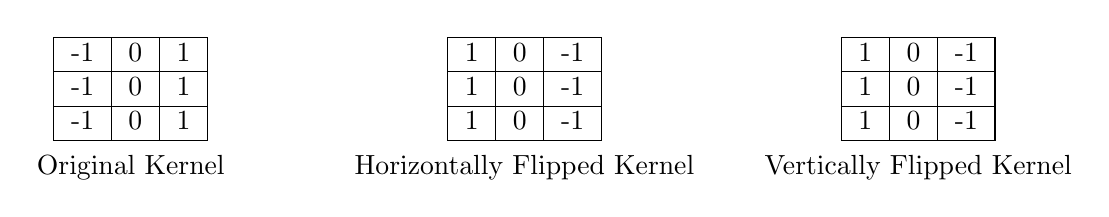
\begin{tikzpicture}
        \begin{scope}[shift={(0,0)}]
            \node at (3.5,0) {
                \begin{tabular}{|c|c|c|}
                    \hline
                    -1 & 0 & 1 \\
                    \hline
                    -1 & 0 & 1 \\
                    \hline
                    -1 & 0 & 1 \\
                    \hline
                \end{tabular}
            };
            \node at (3.5,-1) {Original Kernel};
        \end{scope}
        \begin{scope}[shift={(5,0)}]
            \node at (3.5,0) {
                \begin{tabular}{|c|c|c|}
                    \hline
                    1 & 0 & -1 \\
                    \hline
                    1 & 0 & -1 \\
                    \hline
                    1 & 0 & -1 \\
                    \hline
                \end{tabular}
            };
            \node at (3.5,-1) {Horizontally Flipped Kernel};
        \end{scope}
        \begin{scope}[shift={(10,0)}]
            \node at (3.5,0) {
                \begin{tabular}{|c|c|c|}
                    \hline
                    1 & 0 & -1 \\
                    \hline
                    1 & 0 & -1 \\
                    \hline
                    1 & 0 & -1 \\
                    \hline
                \end{tabular}
            };
            \node at (3.5,-1) {Vertically Flipped Kernel};
        \end{scope}
    \end{tikzpicture}
    \item Slide over the inversed kernel centered at the interested point in the image.
    \item Multiply the inversed kernel data with the overlapped area.
    \item Sum and Accumlate the output values.
\end{enumerate}
\newpage
\begin{egBox}{Example 8.5.2}{}
    \raggedright
    \textbf{Question:}\\
    Given the following input image $I$ and image kernel $K$.
    \begin{center}
        \begin{tabular}{|c|c|c|c|c|}
            \multicolumn{5}{c}{\textbf{Input Image $I$}} \\
            \hline
            10 & 1 & 3 & 2 & 6 \\
            \hline
            4 & 3 & 5 & 8 & 0 \\
            \hline
            8 & 7 & 9 & 6 & 5 \\
            \hline
        \end{tabular}
        \hspace{1cm}
        \begin{tabular}{|m{0.55cm}|m{0.55cm}|m{0.55cm}|}
            \multicolumn{3}{c}{\textbf{Image Kernel $K$}} \\
            \hline
            -1 & 0 & 1 \\
            \hline
            -1 & 0 & 1 \\
            \hline
            -1 & 0 & 1 \\
            \hline
        \end{tabular}
    \end{center}
    Find the output image $O$ after applying the convolution operation.\\
    \vspace{1.5mm}
    \textbf{Answer:}\\
    By using the formula for Image Convolution \(O(x,y) = \sum_{m=-1}^{1} \sum_{n=-1}^{1} K(m,n) \cdot I(x-m, y-n)\), we can find the output image $O$ as follows:
    \begin{align*}
        O(1,1) &= \sum_{m=-1}^{1} \sum_{n=-1}^{1} K(m,n) \cdot I(1-m, 1-n)\\
        &= K(-1,-1) \cdot I(2,2) + K(-1,0) \cdot I(2,1) + K(-1,1) \cdot I(2,0) + K(0,-1) \cdot I(1,2) + K(0,0) \cdot I(1,1) + K(0,1) \cdot I(1,0)\\
        &+ K(1,-1) \cdot I(0,2) + K(1,0) \cdot I(0,1) + K(1,1) \cdot I(0,0)\\
        &= (-1)(9) + (-1)(5) + (-1)(3) + (0)(7) + (0)(3) + (0)(1) + (1)(8) + (1)(4) + (1)(10)\\
        &= -9 - 5 - 3 + 0 + 0 + 0 + 8 + 4 + 10 = \underline{\underline{5}}
    \end{align*}
    \begin{align*}
        O(2,1) &= \sum_{m=-1}^{1} \sum_{n=-1}^{1} K(m,n) \cdot I(2-m, 1-n)\\
        &= K(-1,-1) \cdot I(3,2) + K(-1,0) \cdot I(3,1) + K(-1,1) \cdot I(3,0) + K(0,-1) \cdot I(2,2) + K(0,0) \cdot I(2,1) + K(0,1) \cdot I(2,0)\\
        &+ K(1,-1) \cdot I(1,2) + K(1,0) \cdot I(1,1) + K(1,1) \cdot I(1,0)\\
        &= (-1)(6) + (-1)(8) + (-1)(2) + (0)(9) + (0)(5) + (0)(3) + (1)(7) + (1)(3) + (1)(1)\\
        &= -6 - 8 - 2 + 0 + 0 + 0 + 7 + 3 + 1 = \underline{\underline{-5}}
    \end{align*}
    \begin{align*}
        O(3,1) &= \sum_{m=-1}^{1} \sum_{n=-1}^{1} K(m,n) \cdot I(3-m, 1-n)\\
        &= K(-1,-1) \cdot I(4,2) + K(-1,0) \cdot I(4,1) + K(-1,1) \cdot I(4,0) + K(0,-1) \cdot I(3,2) + K(0,0) \cdot I(3,1) + K(0,1) \cdot I(3,0)\\
        &+ K(1,-1) \cdot I(2,2) + K(1,0) \cdot I(2,1) + K(1,1) \cdot I(2,0)\\
        &= (-1)(5) + (-1)(0) + (-1)(6) + (0)(6) + (0)(8) + (0)(2) + (1)(9) + (1)(5) + (1)(3)\\
        &= -5 - 0 - 6 + 0 + 0 + 0 + 9 + 5 + 3 = \underline{\underline{6}}
    \end{align*}
    $\therefore$ The output image $O$ after applying the convolution operation is:
    \begin{center}
        \textcolor{red}{
            \begin{tabular}{|c|c|c|}
                \hline
                5 & -5 & 6 \\
                \hline
            \end{tabular}
        }
    \end{center}
\end{egBox}
\subsection{Off the Edge Handling of Image Convolution}
\underline{\textbf{Problem:}} When computing an \textcolor{cyan}{output pixel at the boundary of the imags}, the portion of convolution is \textcolor{red}{off the edge of the image}.\\
\begin{center}
    \includegraphics[scale=0.24]{chapter 8/ch8_figure9.jpeg}
\end{center}
\newpage
\underline{\textbf{Solutions:}} We can handle this by:
\begin{enumerate}
    \item \textcolor{cyan}{Zero Padding}: Add a border of pixels all with value zero around the edges of the input images.
    \begin{table}[H]
        \centering
        \newcommand{\myline}{\cline{2-6}}
        \newcommand{\noline}[1]{\multicolumn{1}{c}{#1}}
        \begin{tabular}{c|c|c|c|c|c|c}
            \noline{0} & \noline{0} & \noline{0} & \noline{0} & \noline{0} & \noline{0} & \noline{0} \\
            \myline
            0 & 10 & 1 & 3 & 2 & 6 & 0 \\
            \myline
            0 & 4 & 3 & 5 & 8 & 0 & 0 \\
            \myline
            0 & 8 & 7 & 9 & 6 & 5 & 0 \\
            \myline
            \noline{0} & \noline{0} & \noline{0} & \noline{0} & \noline{0} & \noline{0} & \noline{0} \\
        \end{tabular}
    \end{table}
    \item \textcolor{cyan}{Replicating Boundary Pixels}: Replicate the boundary pixels of the input image to create a border around the image.
    \begin{table}[H]
        \centering
        \newcommand{\myline}{\cline{2-6}}
        \newcommand{\noline}[1]{\multicolumn{1}{c}{#1}}
        \begin{tabular}{c|c|c|c|c|c|c}
            \noline{10} & \noline{10} & \noline{1} & \noline{3} & \noline{2} & \noline{6} & \noline{6} \\
            \myline
            10 & 10 & 1 & 3 & 2 & 6 & 6 \\
            \myline
            4 & 4 & 3 & 5 & 8 & 0 & 0 \\
            \myline
            8 & 8 & 7 & 9 & 6 & 5 & 5 \\
            \myline
            \noline{8} & \noline{8} & \noline{7} & \noline{9} & \noline{6} & \noline{5} & \noline{5} \\
        \end{tabular}
    \end{table}
    \item \textcolor{cyan}{Reflecting Boundary Pixels}: Reflect the boundary pixels of the input image to create a border around the image.
    \begin{table}[H]
        \centering
        \newcommand{\myline}{\cline{2-6}}
        \newcommand{\noline}[1]{\multicolumn{1}{c}{#1}}
        \begin{tabular}{c|c|c|c|c|c|c}
            \noline{10} & \noline{10} & \noline{1} & \noline{3} & \noline{2} & \noline{6} & \noline{6} \\
            \myline
            10 & 10 & 1 & 3 & 2 & 6 & 6 \\
            \myline
            4 & 4 & 3 & 5 & 8 & 0 & 0 \\
            \myline
            8 & 8 & 7 & 9 & 6 & 5 & 5 \\
            \myline
            \noline{8} & \noline{8} & \noline{7} & \noline{9} & \noline{6} & \noline{5} & \noline{5} \\
        \end{tabular}
    \end{table}
    \item \textcolor{cyan}{Mirroring Boundary Pixels}: Mirror the boundary pixels of the input image to create a border around the image.
    \begin{table}[H]
        \centering
        \newcommand{\myline}{\cline{2-6}}
        \newcommand{\noline}[1]{\multicolumn{1}{c}{#1}}
        \begin{tabular}{c|c|c|c|c|c|c}
            \noline{3} & \noline{4} & \noline{3} & \noline{5} & \noline{8} & \noline{0} & \noline{8} \\
            \myline
            1 & 10 & 1 & 3 & 2 & 6 & 2 \\
            \myline
            3 & 4 & 3 & 5 & 8 & 0 & 8 \\
            \myline
            7 & 8 & 7 & 9 & 6 & 5 & 6 \\
            \myline
            \noline{3} & \noline{4} & \noline{3} & \noline{5} & \noline{8} & \noline{0} & \noline{8} \\
        \end{tabular}
    \end{table}
\end{enumerate}
\subsection{Image Convolution in Python}
To perform Image Convolution in Python, we need to first use the \textcolor{cyan}{\texttt{cv2}} module:
\begin{lstlisting}[language=Python, basicstyle=\ttfamily\small, keywordstyle=\color{blue}, commentstyle=\color{forestgreen}, stringstyle=\color{red}, showstringspaces=false]
                                            import cv2
\end{lstlisting}
After that, use the \textcolor{cyan}{\texttt{filter2D()}} method of the \textcolor{violet}{\texttt{cv2}} module to perform Image Convolution.\\
(\textcolor{violet}{\texttt{filter2D()}} \textcolor{cyan}{does not mirror} the image kernel, so we need to \textcolor{cyan}{flip the kernel} before applying the convolution operation):
\begin{synBox}{Syntax 8.5}{Image Convolution in OpenCV}
    \raggedright
    \begin{lstlisting}[language=Python, basicstyle=\ttfamily\small, keywordstyle=\color{blue}, commentstyle=\color{forestgreen}, stringstyle=\color{red}, showstringspaces=false]
        cv2.filter2D(src, ddepth, kernel, dst, anchor, delta, borderType=cv2.BORDER_DEFAULT)
    \end{lstlisting}
    where:
    \begin{itemize}
        \item \textcolor{brown}{\texttt{src}}: Input Image that we want to convolve.
        \item \textcolor{brown}{\texttt{ddepth}}: Desired Depth of the Output Image (If it is set to \textcolor{violet}{\texttt{-1}}, the output image will have the same depth as the input image).
        \item \textcolor{brown}{\texttt{kernel}}: Convolution Kernel (A single-channel floating point matrix).\\
        If we want to apply different kernels to different channels, we can use the \textcolor{violet}{\texttt{cv2.split()}} method to split the image into separate color planes (by splitting and processing each channel separately).
        \item \textcolor{brown}{\texttt{dst}}: Output Image after applying the convolution operation (Same Size and Same Number of Channels as the Input Image).
        \item \textcolor{brown}{\texttt{anchor}}: Anchor of the Kernel that indicates the relative position of a filtered point within the kernel. The anchor should lie within the kernel.\\
        Default value is \textcolor{violet}{\texttt{(-1,-1)}} which means that the anchor is at the kernel center.
        \item \textcolor{brown}{\texttt{delta}}: Optional Value added to the filtered pixels before storing them in the output image.
        \item \textcolor{brown}{\texttt{borderType}}: Pixel extrapolation method.
        \begin{itemize}
            \item \textcolor{violet}{\texttt{cv2.BORDER\_CONSTANT}}: Adds a constant colored border.
            \item \textcolor{violet}{\texttt{cv2.BORDER\_REPLICATE}}: Replicates the last element.
            \item \textcolor{violet}{\texttt{cv2.BORDER\_REFLECT}}: Reflects the elements.
            \item \textcolor{violet}{\texttt{cv2.BORDER\_REFLECT\_101}}: Reflects the elements with a slight change (Same as \texttt{cv2.BORDER\_REFLECT}).
        \end{itemize}
        \item \textcolor{brown}{\texttt{Return Value}}: Filtered Image.
    \end{itemize}
\end{synBox}
\begin{egBox}{Example 8.5.4}{}
    \begin{lstlisting}[language=Python, basicstyle=\ttfamily\small, keywordstyle=\color{blue}, commentstyle=\color{forestgreen}, stringstyle=\color{red}, showstringspaces=false]
from google.colab import drive                      # Import drive from google.colab package
import os, sys                                      # Import os and sys modules

drive.mount('/content/drive')                       # Mount Google Drive
# Assume a folder "images" has been created, go to the folder "images"
os.chdir('/content/drive/My Drive/images')
sys.path.append('/content/drive/My Drive/images')   # Add the path for interpreter to search

# Import all the required libraries
import cv2; import numpy as np
import matplotlib.image as mpimg; import matplotlib.pyplot as plt

img = mpimg.imread('snorlax-sleep.png')             # Read the image

# Convert the color image to gray and show it
grayImg = cv2.cvtColor(img, cv2.COLOR_RGB2GRAY)
plt.figure(); plt.imshow(grayImg, cmap='gray', vmin=0, vmax=1)

# Prepare a kernel (a sharpening kernel here)
kernel_3x3 = np.array([[0, -1, 0], [-1, 5, -1], [0, -1, 0]])

for i in range(5): # Perform filtering 5 times
    grayImg = cv2.filter2D(grayImg, -1, kernel_3x3)

# Show the resulting image
plt.figure(); plt.imshow(grayImg, cmap="gray", vmin=0, vmax=1)

# Output: <matplotlib.image.AxesImage at 0x7faf40dc9e50>
    \end{lstlisting}
    \begin{center}
        \begin{tikzpicture}[node distance=6.5cm]
            \node (snorlax_sleep_gray) {\includegraphics[scale=0.4]{chapter 8/snorlax_sleep_gray.png}};
            \node (snorlax_sleep_sharpened) [right of=snorlax_sleep_gray] {\includegraphics[scale=0.4]{chapter 8/snorlax_sleep_gray_convolution.png}
            };

            \node [above of=snorlax_sleep_gray, node distance=1.7cm] {\textbf{Input Image}};
            \node [above of=snorlax_sleep_sharpened, node distance=1.7cm] {\textbf{Output Sharpened Image}};

            \draw[->, line width=0.5mm] (snorlax_sleep_gray) -- (snorlax_sleep_sharpened);
        \end{tikzpicture}
    \end{center}
\end{egBox}
\textcolor{magenta}{\section{\textbf{Image Kernels}}}
\subsection{Introduction to Image Kernels}
\begin{defBox}{Definition 8.6.1}{Image Kernels}
    \textcolor{cyan}{Image Kernels} are the \textcolor{red}{small matrices used for image processing operations} such as smoothing, sharpening, edge detection, and more.
\end{defBox}
Here are the most common types of Image Kernels:
\begin{itemize}
    \item \textcolor{cyan}{\textbf{Smoothing/Averaging/Blurring Kernels}}.
    \item \textcolor{cyan}{\textbf{Identity Kernels}}.
    \item \textcolor{cyan}{\textbf{Edge Detection Kernels}}.
    \item \textcolor{cyan}{\textbf{Sharpening Kernels}}.
    \item \textcolor{cyan}{\textbf{Prewitt Kernels}}.
    \item \textcolor{cyan}{\textbf{Sobel Kernels}}.
    \item \textcolor{cyan}{\textbf{Shifted Identity Kernels}}.
\end{itemize}
\newpage
\subsection{Smoothing/Averaging/Blurring Kernels}

\textcolor{cyan}{Smoothing/Averaging/Blurring images} can be done by \textcolor{violet}{averaging pixels} (Analogous to integration related to the sum of pixel intensity values).\\
Kernels used for Smoothing/Averaging/Blurring are \textcolor{red}{Box Blur Kernels}:
\begin{center}
    \textcolor{red}{
    \begin{tabular}{|c|c|c|}
        \hline
        {\large $\frac{1}{9}$} & {\large $\frac{1}{9}$} & {\large $\frac{1}{9}$} \\
        \hline
        {\large $\frac{1}{9}$} & {\large $\frac{1}{9}$} & {\large $\frac{1}{9}$} \\
        \hline
        {\large $\frac{1}{9}$} & {\large $\frac{1}{9}$} & {\large $\frac{1}{9}$} \\
        \hline
    \end{tabular}}
\end{center}
Effects of Smoothing/Averaging/Blurring Kernels in Different Sizes:
\begin{center}
    \includegraphics[scale=0.27]{chapter 8/smoothing_kernel.jpeg}
\end{center}
\subsection{Identity Kernels}
\textcolor{cyan}{Identity Kernels} are used to keep the image the same (\textcolor{violet}{No Change in the image}).\\
$\Rightarrow$ Convolve the original image with the Identity Kernel $n$ times will still result in the original image.\\
Identity Kernels are represented as:
\begin{center}
    \textcolor{red}{
    \begin{tabular}{|c|c|c|}
        \hline
        0 & 0 & 0 \\
        \hline
        0 & 1 & 0 \\
        \hline
        0 & 0 & 0 \\
        \hline
    \end{tabular}}
\end{center}
\begin{center}
    \begin{tikzpicture}[node distance=6.5cm]
        \node (dog_original) {\includegraphics[scale=0.18]{chapter 8/dog-original.png}};
        \node (dog_identity) [right of=dog_original] {\includegraphics[scale=0.18]{chapter 8/dog-original.png}
        };

        \node [above of=dog_original, node distance=2cm] {\textbf{Original Image}};
        \node [above of=dog_identity, node distance=2cm] {\textbf{Identity Image}};

        \draw[->, line width=0.5mm] (dog_original) -- (dog_identity);
    \end{tikzpicture}
\end{center}
\subsection{Edge Detection Kernels}
\textcolor{cyan}{Edge Detection Kernels} are used to \textcolor{violet}{detect the edges of objects or regions within an image}.\\
Edge Detection Kernels are represented as:
\begin{center}
    \textcolor{red}{
    \begin{tabular}{|c|c|c|}
        \hline
        -1 & -1 & -1 \\
        \hline
        -1 & 8 & -1 \\
        \hline
        -1 & -1 & -1 \\
        \hline
    \end{tabular}}
\end{center}
\subsection{Sharpening Kernels}
\textcolor{cyan}{Sharpening Kernels} are used to \textcolor{violet}{remove blur, enhance details, and dehaze the image}.\\
It has the opposite effect of smoothing (Analogous to differentiation related to the difference of pixel intensity values).\\
Sharpening Kernels are represented as:
\begin{center}
    \textcolor{red}{
    \begin{tabular}{|c|c|c|}
        \hline
        -1 & -1 & -1 \\
        \hline
        -1 & 9 & -1 \\
        \hline
        -1 & -1 & -1 \\
        \hline
    \end{tabular}}
\end{center}
\begin{center}
    \includegraphics[scale=0.3]{chapter 8/sharpening_kernel.jpeg}
\end{center}
\newpage
\subsection{Prewitt Kernels}
Kernels used for \textcolor{cyan}{Prewitt Edge Detection} are:
\begin{itemize}
    \item \textcolor{red}{Prewitt Kernel for Horizontal Edge Detection}:
    \begin{center}
        \textcolor{red}{
        \begin{tabular}{|c|c|c|}
            \hline
            -1 & -1 & -1 \\
            \hline
            0 & 0 & 0 \\
            \hline
            1 & 1 & 1 \\
            \hline
        \end{tabular}}
    \end{center}
    \item \textcolor{red}{Prewitt Kernel for Vertical Edge Detection}:
    \begin{center}
        \textcolor{red}{
        \begin{tabular}{|c|c|c|}
            \hline
            -1 & 0 & 1 \\
            \hline
            -1 & 0 & 1 \\
            \hline
            -1 & 0 & 1 \\
            \hline
        \end{tabular}}
    \end{center}
\end{itemize}
\begin{center}
    \includegraphics[scale=0.3]{chapter 8/prewitt_kernel.jpeg}
\end{center}
\subsection{Sobel Kernels}
Kernels used for \textcolor{cyan}{Sobel Edge Detection} are:
\begin{itemize}
    \item \textcolor{red}{Sobel Kernel for Horizontal Edge Detection}:
    \begin{center}
        \textcolor{red}{
        \begin{tabular}{|c|c|c|}
            \hline
            -1 & -2 & -1 \\
            \hline
            0 & 0 & 0 \\
            \hline
            1 & 2 & 1 \\
            \hline
        \end{tabular}}
    \end{center}
    \item \textcolor{red}{Sobel Kernel for Vertical Edge Detection}:
    \begin{center}
        \textcolor{red}{
        \begin{tabular}{|c|c|c|}
            \hline
            -1 & 0 & 1 \\
            \hline
            -2 & 0 & 2 \\
            \hline
            -1 & 0 & 1 \\
            \hline
        \end{tabular}}
    \end{center}
\end{itemize}
\begin{center}
    \includegraphics[scale=0.3]{chapter 8/sobel_kernel.jpeg}
\end{center}
\subsection{Shifted Identity Kernels}
\textcolor{cyan}{Shifted Identity Kernels} are used to \textcolor{violet}{shift the image in a particular direction}.\\
$\Rightarrow$ Convolve the original image with the Shifted Identity Kernel $n$ times will shift the image in that direction for $n$ pixels.\\
Shifted Identity Kernels are represented as:
\begin{center}
    \textcolor{red}{
    \begin{tabular}{|c|c|c|}
        \hline
        0 & 0 & 0 \\
        \hline
        1 & 0 & 0 \\
        \hline
        0 & 0 & 0 \\
        \hline
    \end{tabular}}
\end{center}
\begin{center}
    \begin{tikzpicture}[node distance=6.5cm]
        \node (dog_original) {\includegraphics[scale=0.18]{chapter 8/dog-original.png}};
        \node (dog_shifted) [right of=dog_original] {\includegraphics[scale=0.15]{chapter 8/shifted_kernel_dog.jpeg}
        };

        \node [above of=dog_original, node distance=2cm] {\textbf{Original Image}};
        \node [above of=dog_shifted, node distance=2.05cm] {\textbf{Shifted Image}};

        \draw[->, line width=0.5mm] (dog_original) -- (dog_shifted);
    \end{tikzpicture}
\end{center}
\newpage
\textbf{\textcolor{purple}{\Large{Practice Problem}}}\\
A 3-bit/pixel (Pixel Value is in the range of $0$ to $2^3 = 8$) image of size $3 \times 3$ is given below as:
\begin{center}
    \begin{tabular}{|c|c|c|}
        \hline
        3 & 7 & 6 \\
        \hline
        2 & 4 & 6 \\
        \hline
        4 & 7 & 2 \\
        \hline
    \end{tabular}
\end{center}
\textbf{Question 1:} Find the output of a $3 \times 3$ averaging kernel at $(1,1)$ .\\
\textbf{Answer:} The output value of the $3 \times 3$ averaging kernel at $(1,1)$ is given by:
\[
    O(1,1) = \frac{1}{9} \left(3 + 7 + 6 + 2 + 4 + 6 + 4 + 7 + 2\right) = \underline{\underline{\frac{41}{9}}}
\]
\textbf{Question 2:} Find the edge magnitude at $(1,1)$ using the Sobel masks shown below after applying the convolution operation.\\
    \begin{center}
        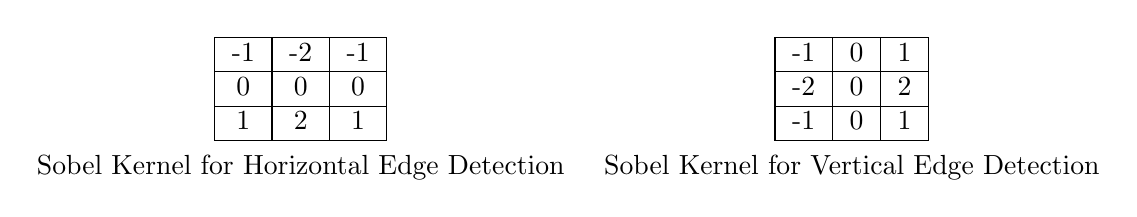
\begin{tikzpicture}
            \begin{scope}[shift={(0,0)}]
                \node at (3.5,0) {
                    \begin{tabular}{|c|c|c|}
                        \hline
                        -1 & -2 & -1 \\
                        \hline
                        0 & 0 & 0 \\
                        \hline
                        1 & 2 & 1 \\
                        \hline
                    \end{tabular}
                };
                \node at (3.5,-1) {Sobel Kernel for Horizontal Edge Detection};
            \end{scope}
            \begin{scope}[shift={(7,0)}]
                \node at (3.5,0) {
                    \begin{tabular}{|c|c|c|}
                        \hline
                        -1 & 0 & 1 \\
                        \hline
                        -2 & 0 & 2 \\
                        \hline
                        -1 & 0 & 1 \\
                        \hline
                    \end{tabular}
                };
                \node at (3.5,-1) {Sobel Kernel for Vertical Edge Detection};
            \end{scope}
        \end{tikzpicture}
    \end{center}
    (Note: \(\text{Edge Magnitude} = \sqrt{(\text{Horizontal Edge Value})^2 + (\text{Vertical Edge Value})^2}\))\\
\textbf{Answer:}\\
The horizontal edge value at $(1,1)$ is given by:
\[
    \text{Horizontal Edge Value} = (1)(3) + (2)(7) + (1)(6) + (0)(2) + (0)(4) + (0)(6) + (-1)(4) + (-2)(7) + (-1)(2) = 3 + 14 + 6 - 4 - 14 - 2 = 3
\]
The vertical edge value at $(1,1)$ is given by:
\[
    \text{Vertical Edge Value} = (1)(3) + (0)(7) + (-1)(6) + (2)(2) + (0)(4) + (-2)(6) + (1)(4) + (0)(7) + (-1)(2) = 3 - 6 + 4 - 12 + 4 - 2 = -9
\]
The edge magnitude at $(1,1)$ is given by:
\[
    \text{Edge Magnitude} = \sqrt{(3)^2 + (-9)^2} = \sqrt{9 + 81} = \sqrt{90} = \underline{\underline{3\sqrt{10}}} \approx 9.49
\]

\chapter{Convolutional Neural Networks (CNNs)}
\textcolor{magenta}{\section{\textbf{Introduction to Convolutional Neural Networks (CNNs)}}}
\subsection{Definition of Convolutional Neural Networks (CNNs)}
\begin{defBox}{Definition 9.1}{Convolutional Neural Networks (CNNs)}
    \textcolor{cyan}{Convolutional Neural Networks (CNNs/ConvNet)} are neural networks \textcolor{red}{with a convolution operation in at least one of the layers}.\\
    $\Rightarrow$ A class of Artificial Neural Networks (ANNs) \textcolor{violet}{applied to analyze visual imagery}.
\end{defBox}
\begin{center}
    \includegraphics[scale=0.23]{chapter 9/ch9_figure1.jpeg}
\end{center}
CNNs were developed in the late 1980s and then forgotten due to the lack of processing power.\\
However, CNNs and deep learning have become popular in the last decade due to the availability of \textcolor{violet}{large datasets} and \textcolor{violet}{powerful Graphical Processing Units (GPUs)}.\\
Some research states that preprocessing images before feeding them into a CNN can \textcolor{violet}{significantly improve the classification/recognition accuracy}.\\
\vspace{2mm}
There are a lot of applications of CNNs, such as natural language processing, speech recognition, recommendation systems, image segmentation, medical image analysis, financial time series forecasting, playing games, and more.
\subsection{Steps of Feeding Convolutions in CNNs}
The steps of feeding convolutions in CNNs are as follows:
\begin{enumerate}
    \item Recognize that \textcolor{violet}{every pixel in an image is a feature/input node}.
    \item \textcolor{cyan}{Result from each convolution} is placed into the \textcolor{violet}{next layer in the hidden node}.\\
    (Each feature/pixel of the convolved image is a node in the hidden layer.)
    \item \textcolor{cyan}{Numbers in the kernel} are \textcolor{violet}{weights connecting the the feature of the input image and the hidden node} which needs to be \textcolor{violet}{learned during training}.
\end{enumerate}
\newpage
\begin{center}
    \includegraphics[scale=0.24]{chapter 9/ch9_figure2.jpeg}
    \hspace{0.5cm}
    \includegraphics[scale=0.23]{chapter 9/ch9_figure3.jpeg}
\end{center}
\subsection{Brief Diagram of Convolutional Neural Networks (CNNs)}
There are \textcolor{violet}{three main types of layers} with input and output layers in Convolutional Neural Networks (CNNs):
\begin{enumerate}
    \item \textcolor{cyan}{\textbf{Convolutional Layer}}: The layer where the \textcolor{violet}{convolution operation is performed}.
    \item \textcolor{cyan}{\textbf{Pooling Layer}}: The layer where the \textcolor{violet}{downsampling operation is performed}.
    \item \textcolor{cyan}{\textbf{Fully-Connected Layer}}: The layer where the \textcolor{violet}{neurons are connected to all the neurons in the previous layer}.
\end{enumerate}
\begin{center}
    \includegraphics[scale=0.23]{chapter 9/ch9_figure4.jpeg}
\end{center}
\textcolor{magenta}{\section{\textbf{Types of Layers in Convolutional Neural Networks (CNNs)}}}
\subsection{Input Layer}
\begin{defBox}{Definition 9.2.1}{Input Layer}
    The \textcolor{cyan}{Input Layer} is the first layer of the Convolutional Neural Network (CNN) where the \textcolor{red}{input image is placed in this layer} which can be \textcolor{violet}{single-layer 2D images (grayscale)}, \textcolor{violet}{3-channel 2D images (RGB)} or \textcolor{violet}{3D}.
\end{defBox}
\textcolor{cyan}{Kernels} in the \textcolor{violet}{same depth as the input} need to be learned.
\begin{center}
    \includegraphics[scale=0.21]{chapter 9/ch9_figure5.jpeg}
\end{center}
\newpage
\subsection{Convolutional Layer}
\textcolor{olive}{\subsubsection{Diagram of Convolutional Layer}}
Assumption: Ignore those pixels that cannot have 24 neighboring pixels.\\
Inputs: $28 \times 28 \times 3$ Image and $10 \times 5 \times 5 \times 3$ Kernel.\\
Output: $24 \times 24 \times 10$ Convolved Image.
\begin{center}
    \includegraphics[scale=0.17]{chapter 9/ch9_figure6.jpeg}
    \includegraphics[scale=0.23]{chapter 9/ch9_figure7.jpeg}
\end{center}
\textcolor{olive}{\subsubsection{Stride}}
\begin{defBox}{Definition 9.2.2.2}{Stride}
    \textcolor{cyan}{Stride} is the \textcolor{red}{amount of movement} between applications of the kernel to the input image.
\end{defBox}
The \textcolor{cyan}{default stride/strides in 2D} is \textcolor{red}{$(1,1)$} for the height and the width movement.\\
The kernel is moved across the image \textcolor{violet}{left to right top to bottom, with a one-pixel column change on the horizontal movements and then a one-pixel row change on the vertical movements}.\\
The stride can be changed, affecting on how kernel is applied to both the image and the size of the resulting output image.\\
The stride can be specified in Keras on the \textcolor{violet}{\texttt{Conv2D()}} layer as the \textcolor{violet}{\texttt{strides}} parameter by specifying a tuple of height and width strides.\\
\fbox{
    \parbox{0.97\textwidth}{
        Reasons why the stride is \textcolor{red}{set to a larger value}:
        \begin{itemize}
            \item Lesser overlaps for \textcolor{cyan}{lower output volume}.
            \item \textcolor{cyan}{Lesser memory} needed for output.
            \item \textcolor{cyan}{Avoids overfitting} when the image processing has a large number of attributes.
        \end{itemize}
    }
}\\
\vspace{1mm}
\begin{thmBox}{Theorem 9.2.2.2}{Formula for Determining the Output Size of Convolutional Layer}
    The \textcolor{red}{output size of the Convolutional Layer} can be determined using the formula:
    \[
        \text{Output Size} = \frac{\text{Size of Image Dimension} - \text{Size of Kernel Dimension}}{\text{Stride}} + 1
    \]
\end{thmBox}
\uline{Example of Spatial Dimensions of Convolutional Layer with Stride}:\\
Suppose we have a $7 \times 7$ image and a $3 \times 3$ kernel for performing convolution.\\
\begin{enumerate}
    \item \textcolor{cyan}{Stride of 1}: Output Size = $\frac{7 - 3}{1} + 1 = 5$.\\
    $\Rightarrow$ The output size of the Convolutional Layer is $5 \times 5$.
    \item \textcolor{cyan}{Stride of 2}: Output Size = $\frac{7 - 3}{2} + 1 = 3$.\\
    $\Rightarrow$ The output size of the Convolutional Layer is $3 \times 3$.
    \item \textcolor{cyan}{Stride of 3}: Output Size = $\frac{7 - 3}{3} + 1 = 2.33$.\\
    Cannot apply a stride of 3 as it does not fit (Not reaching the input image boundary).
\end{enumerate}
\textcolor{olive}{\subsubsection{Zero Padding}}
When a kernel \textcolor{cyan}{convolves a given input image}, the \textcolor{violet}{dimensions of the output image are reduced}.
To preserve the size of the output image, we can add \textcolor{red}{zero padding} to the input image.\\
\begin{defBox}{Definition 9.2.2.3}{Zero Padding}
    \textcolor{cyan}{Zero Padding} occurs when we \textcolor{red}{add a border of pixels all with value zero around the boundaries of the input images}.
\end{defBox}
\newpage
For implementation of CNNs using Keras, there are two types of padding:
\begin{itemize}
    \item \textcolor{cyan}{\textbf{Valid Padding}}: No padding is added to the input image.
    \item \textcolor{cyan}{\textbf{Same Padding}}: Padding the original input with zeros before applying the convolution operation to maintain the output size same as the input size.
\end{itemize}
\begin{thmBox}{Theorem 9.2.2.3}{Numbers of Zero Padding to Maintain Output Size}
    Assuming the stride is 1, to maintain the output size of the Convolutional Layer, the number of zero padding to be added to the input image can be determined using the formula:
    \[
        \text{Number of Zero Padding} = \frac{\text{Size of Kernel Dimension} - 1}{2}
    \]
\end{thmBox}
\uline{Example of Zero Padding to Maintain Output Size:}\\
\begin{itemize}
    \item If \(K = 3\), then the number of zero padding to maintain the output size is \(\frac{3 - 1}{2} = 1 \text{ pixel border}\).
    \item If \(K = 5\), then the number of zero padding to maintain the output size is \(\frac{5 - 1}{2} = 2 \text{ pixel border}\).
    \item If \(K = 7\), then the number of zero padding to maintain the output size is \(\frac{7 - 1}{2} = 3 \text{ pixel border}\).
\end{itemize}
\textcolor{olive}{\subsubsection{Non-Linearity Activation Function}}
We need \textcolor{red}{non-linearity activation functions} in the Convolutional Layer to \textcolor{violet}{prevent two linear convolution operations from being equivalent to a single linear operation} (no more powerful than a single layer).\\
The non-lineary is NOT its own layer, but is a part of the Convolutional Layer as it is done in neurons.\\
\textcolor{cyan}{Rectified Linear Unit (ReLU) is more popular for CNNs} than Sigmoid and Tanh functions since it does \textcolor{violet}{not require any expensive consumption}.\\
$\Rightarrow$ Shown to \textcolor{violet}{speed up the convergence of stochastic gradient descent (SGD) algorithms}.\\
\textcolor{olive}{\subsubsection{Example of Convolutional Layer}}
\begin{egBox}{Example 9.2.2}{}
    \raggedright
    Suppuse we have an input image size of $32 \times 32 \times 3$ and 10 kernels of size $5 \times 5 \times 3$ with stride 1.\\
    \begin{itemize}
        \item Zero Padding: \textcolor{red}{2 pixels border}.
        \item Output Size = $\frac{32 + 2(2) - 5}{1} + 1 = 32$.
        \item Output Size of Convolutional Layer: $32 \times 32 \times 10$.
        \item Number of Parameters:
        \item Each kernel has $5 \times 5 \times 3 + 1 = 76$ parameters (75 weights and 1 bias).
    \end{itemize}
    $\therefore$ Total Number of Parameters: $10 \times 76 = \underline{\underline{760}}$.
\end{egBox}
\subsection{Pooling Layer}
\begin{defBox}{Definition 9.2.3}{Pooling Layer}
    The \textcolor{cyan}{Pooling Layer} is the layer where the subsequent layers of the CNN can \textcolor{red}{pick up larger-scale detail} than just edges and curves.
\end{defBox}
It \textcolor{red}{merges pixel regions} in the convolved image together by \textcolor{violet}{shrinking the image} before attempting to learn kernels on it.\\
\vspace{1mm}
\fbox{
    \parbox{0.97\textwidth}{
        \textcolor{red}{Pooling can \textcolor{violet}{tolerate local distortions \& translation of patterns of interest} and \textcolor{violet}{reduce the computational load, memory usage \& the number of parameters}}.
    }
}\\
\begin{center}
    \includegraphics[scale=0.2]{chapter 9/ch9_figure8.jpeg}
\end{center}
\newpage
Two Popular Types of Pooling Layers:
\begin{itemize}
    \item \textcolor{cyan}{\textbf{Max Pooling}}: \textcolor{red}{Applies the maximum filter} to the non-overlapping subregions of the initial representation.
    \item \textcolor{cyan}{\textbf{Average Pooling}}: \textcolor{red}{Applies the average filter} to the non-overlapping subregions of the initial representation.
\end{itemize}
\begin{center}
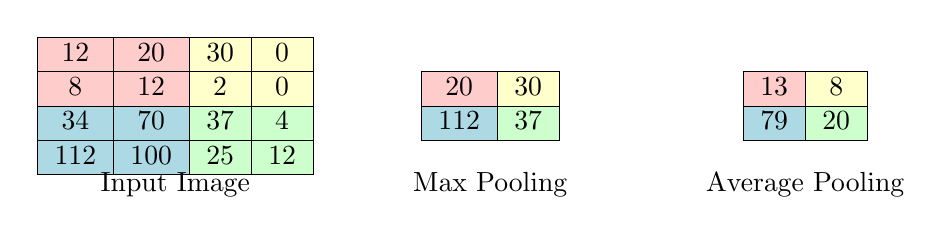
\begin{tikzpicture}
    \begin{scope}[shift={(0,0)}]
        \node at (3.5,0) {
            \begin{tabular}{|c|c|c|c|}
                \hline
                \cellcolor{lightred}{12} & \cellcolor{lightred}{20} & \cellcolor{lightyellow}{30} & \cellcolor{lightyellow}{0} \\
                \hline
                \cellcolor{lightred}{8} & \cellcolor{lightred}{12} & \cellcolor{lightyellow}{2} & \cellcolor{lightyellow}{0} \\
                \hline
                \cellcolor{lightblue}{34} & \cellcolor{lightblue}{70} & \cellcolor{lightgreen}{37} & \cellcolor{lightgreen}{4} \\
                \hline
                \cellcolor{lightblue}{112} & \cellcolor{lightblue}{100} & \cellcolor{lightgreen}{25} & \cellcolor{lightgreen}{12} \\
                \hline
            \end{tabular}
        };
        \node at (3.5,-1) {Input Image};
    \end{scope}
    \begin{scope}[shift={(4,0)}]
        \node at (3.5,0) {
            \begin{tabular}{|c|c|}
                \hline
                \cellcolor{lightred}{20} & \cellcolor{lightyellow}{30} \\
                \hline
                \cellcolor{lightblue}{112} & \cellcolor{lightgreen}{37} \\
                \hline
            \end{tabular}
        };
        \node at (3.5,-1) {Max Pooling};
    \end{scope}
    \begin{scope}[shift={(8,0)}]
        \node at (3.5,0) {
            \begin{tabular}{|c|c|}
                \hline
                \cellcolor{lightred}{13} & \cellcolor{lightyellow}{8} \\
                \hline
                \cellcolor{lightblue}{79} & \cellcolor{lightgreen}{20} \\
                \hline
            \end{tabular}
        };
        \node at (3.5,-1) {Average Pooling};
    \end{scope}
\end{tikzpicture}
\end{center}
\subsection{Fully-Connected/Dense Layer}
\begin{defBox}{Definition 9.2.4}{Fully-Connected/Dense Layer}
    The \textcolor{cyan}{Fully-Connected/Dense Layer} is a \textcolor{red}{traditional multi-layer perceptron} which uses a \textcolor{red}{softmax activation function} in the output layer.
\end{defBox}
It implies that \textcolor{violet}{all the neurons in the previous layer are connected to all the neurons in the current layer}.\\
Purpose of Fully-Connected Layer:\\
\begin{itemize}
    \item \textcolor{cyan}{Acts as a classifier} to use \textcolor{violet}{features extracted by the Convolutional and Pooling Layers} to \textcolor{violet}{classify the input image into various classes} based on the training dataset.
\end{itemize}
$\Rightarrow$ Since the \textcolor{violet}{output from the Convolutional and Pooling Layers} \textcolor{cyan}{acts as feature extractors} from the input image, which represents the \textcolor{cyan}{high-level features} of the input image.\\
\subsection{Dropout Layer}
\textcolor{cyan}{Large neural network trained on relatively small datasets} can \textcolor{violet}{overfit the training data} and \textcolor{violet}{increase the generalization error}.\\
The model \textcolor{cyan}{learning the statistical noise in the training data} results in \textcolor{violet}{poor performance on new data}.\\
To \textcolor{red}{prevent neural networks from overfitting}, the \textcolor{cyan}{Dropout Layer} is used.\\
\begin{defBox}{Definition 9.2.5}{Dropout Layer}
    The \textcolor{cyan}{Dropout Layer} is a \textcolor{red}{regularization technique} where \textcolor{violet}{some number of layer outputs are randomly ignored/"dropped out"} during training.
\end{defBox}
\begin{center}
    \includegraphics[scale=0.15]{chapter 9/ch9_figure9.jpeg}
\end{center}
Effects of Dropout Layer:
\begin{itemize}
    \item Force nodes within the layer to \textcolor{violet}{probabilistically take on more or less responsibility for the inputs}.
    \item Reduces the capacity / Thins the network during training since the output of a layer under dropout are \textcolor{violet}{randomly subsampled}.\\
    $\Rightarrow$ A \textcolor{cyan}{Wider network} may be required when using dropout.
\end{itemize}
Dropout is \textcolor{red}{implemented per-layer} in a neural network:
\begin{itemize}
    \item \textcolor{cyan}{Dense Fully-Connected Layer, Convolutional Layer \& Pooling Layer} can have dropout applied.
    \item \textcolor{cyan}{Hidden layers \& Input layers} may have dropout implemented.
    \item \textcolor{cyan}{Output layer} should \textcolor{violet}{not have dropout} as it is the final layer.
\end{itemize}
\fbox{
    \parbox{0.97\textwidth}{
        \textcolor{cyan}{Dropout rate} is the parameter that \textcolor{red}{probability at which the outputs of the layer are dropped out} during training.\\
        $\Rightarrow$ Dropout rate is commonly set to \textcolor{red}{0.5} for retraining the output of each node in a hidden layer.
    }
}
\textcolor{magenta}{\section{\textbf{Overall Training Process of Convolutional Neural Networks (CNNs)}}}
Here is the overall training process of Convolutional Neural Networks (CNNs):
\begin{enumerate}
    \item \textcolor{red}{Initialize all kernels} and \textcolor{red}{parameters/weights with random values}.
    \item \textcolor{cyan}{Forward Propagation}: Takes the input image for training and \textcolor{red}{passes it through the network (Convolution, ReLU, Pooling, Fully-Connected Layers)} to \textcolor{violet}{find the output probabilities for each class}.
    \item Calculate the \textcolor{cyan}{Total Error at the Output Layer} using the \textcolor{red}{Softmax Activation Function}.
    \item \textcolor{cyan}{Backward Propagation}: \textcolor{red}{Updates all kernel values} and \textcolor{red}{parameters/weights} using the \textcolor{violet}{Gradient Descent Algorithm} to \textcolor{violet}{minimize the output error}.
    \item \textcolor{cyan}{Repeat Steps 2 to 4} for all the training images in the dataset.
\end{enumerate}
\newpage
\textcolor{magenta}{\section{\textbf{Handwritten Digit Recognition using Convolutional Neural Networks (CNNs)}}}
\subsection{Terminologies in Handwritten Digit Recognition using CNNs}
Convolutional Neural Networks (CNNs) is built \textcolor{cyan}{recognize/classify handwritten digits}.
\begin{itemize}
    \item \textcolor{cyan}{\textbf{MNIST Dataset}}: A dataset of \textcolor{violet}{60,000 training images} and \textcolor{violet}{10,000 testing images} of handwritten digits.
    \item \textcolor{cyan}{\textbf{Softmax Activation Function}}: A function that \textcolor{violet}{converts the output of the last layer into probabilities}.
    \item \textcolor{cyan}{\textbf{Cross-Entropy Loss Function}}: A function that \textcolor{violet}{measures the performance of the classification model}.
\end{itemize}
\begin{center}
    \includegraphics[scale=0.27]{chapter 7/ch7_figure12.jpeg}
\end{center}
\subsection{Procedures in Handwritten Digit Recognition using CNNs}
Here are the procedures for recognizing handwritten digits using Convolutional Neural Networks (CNNs):
\begin{enumerate}
    \item Import the required libraries \& Define global variables for the CNN model.
    \item Load the Data from the MNIST Dataset \& Prepare the Data.
    \item Build the Convolutional Neural Network (CNN) Model.
    \item Compile the CNN Model with the Loss Function, Optimizer, and Metrics.
    \item Train the CNN Model using the Training Data.
    \item Evaluate the Model Accuracy using the Testing Data.
    \item Save the Model.
    \item Use the Model to Predict the Handwritten Digits.
\end{enumerate}
\uline{Step 1: Import the Required Libraries \& Define Global Variables for the CNN Model}\\
\vspace{1mm}
The required libraries are imported and the global variables for the CNN model are defined.\\
\vspace{3mm}
\textit{\large Step 1 Code Implementation:}\\
\begin{lstlisting}[language=Python, basicstyle=\ttfamily\small, keywordstyle=\color{blue}, commentstyle=\color{forestgreen}, stringstyle=\color{red}, showstringspaces=false]
import numpy as np                               # Import numpy library
import matplotlib.pyplot as plt                  # Import mathplot library
import datetime                                  # Import datetime library
from keras.datasets import mnist                 # Import MNIST dataset
from keras.models import Sequential              # Import Sequential class
from keras.layers import Conv2D, MaxPooling2D    # Import Conv2D, MaxPooling2D class
from keras.layers import Dense, Dropout, Flatten # Import Dense, Dropout, Flatten class
from keras.utils import to_categorical           # Import numpy-related utilities
from keras.callbacks import TensorBoard          # Import TensorBoard class
from keras.models import load_model              # Import load_model method
from tensorflow.keras.utils import plot_model    # Import plot_model method
from tensorflow.math import confusion_matrix     # Import confusion matrix method
# Import spare categorical crossentroy loss
from tensorflow.keras.metrics import categorical_crossentropy

batch_size = 128                                 # Number of samples per gradient update
num_classes = 10                                 # Number of classes in the dataset
epochs = 1                                       # Number of epochs to train the model
img_rows, img_cols = 28, 28                      # Image dimensions
\end{lstlisting}
\newpage
\uline{Step 2: Load the Data from the MNIST Dataset \& Prepare the Data}\\
\vspace{1mm}
The data is loaded from the MNIST dataset using the \textcolor{violet}{\texttt{load\_data()}} method.
\begin{itemize}
    \item \textcolor{cyan}{\texttt{x\_train}}: NumPy array of grayscale image data with shapes (60000, 28, 28).
    \item \textcolor{cyan}{\texttt{y\_train}}: NumPy array of digit labels (integers in range 0-9) with shape (60000,).
    \item \textcolor{cyan}{\texttt{x\_test}}: NumPy array of grayscale image data with shapes (10000, 28, 28).
    \item \textcolor{cyan}{\texttt{y\_test}}: NumPy array of digit labels (integers in range 0-9) with shape (10000,).
\end{itemize}
Then the data is reshaped and normalized to be fed into the CNN model.
\begin{itemize}
    \item Reshape the \textcolor{violet}{\texttt{x\_train}} and \textcolor{violet}{\texttt{x\_test}} to a 4D array with shape (num\_images, img\_rows, img\_cols, 1).
    \item Transform the \textcolor{violet}{\texttt{y\_train}} and \textcolor{violet}{\texttt{y\_test}} to one-hot encoded vectors (10 element binary vectors with a 1 for the index of the class value and 0 for all other classes) to have 10 classes with unique integers by using the \textcolor{cyan}{\texttt{to\_categorical()}} method.
\end{itemize}
\vspace{1mm}
\textit{\large Step 2 Code Implementation:}\\
\begin{lstlisting}[language=Python, basicstyle=\ttfamily\small, keywordstyle=\color{blue}, commentstyle=\color{forestgreen}, stringstyle=\color{red}, showstringspaces=false]
(x_train, y_train), (x_test, y_test) = mnist.load_data() # Load the MNIST dataset

# Reshape the data to 4D array with shape (num_images, img_rows, img_cols, 1)
x_train = x_train.reshape(60000, 28, 28, 1)
x_test = x_test.reshape(10000, 28, 28, 1)

# Transform the data to one-hot encoded vectors
y_train = to_categorical(y_train, num_classes)
y_test = to_categorical(y_test, num_classes)
\end{lstlisting}
\uline{Step 3: Build the Convolutional Neural Network (CNN) Model}\\
\vspace{1mm}
Instead of building the CNN model from scratch, we will use the \textcolor{red}{software library Keras} to build the CNN model.\\
The CNN model consists of the following layers:
\begin{itemize}
    \item \textcolor{cyan}{Convolutional Layer 1} with \textcolor{violet}{32 kernels of size $3 \times 3$} and Use \textcolor{violet}{ReLU activation function} (Layer 1).
    \begin{itemize}
        \item Padding is set to \textcolor{red}{\texttt{"valid"}} and the strides are set to \textcolor{red}{\texttt{(1,1)}}.
        \item Need to specify the \textcolor{cyan}{input shape}:  \textcolor{red}{\texttt{(28, 28, 1)}} for the first layer only.
    \end{itemize}
    \item \textcolor{cyan}{Convolutional Layer 2} with \textcolor{violet}{64 kernels of size $3 \times 3$} and Use \textcolor{violet}{ReLU activation function} (Layer 2).
    \begin{itemize}
        \item Padding is set to \textcolor{red}{\texttt{"valid"}} and the strides are set to \textcolor{red}{\texttt{(1,1)}}.
    \end{itemize}
    \item \textcolor{cyan}{Max Pooling Layer} with \textcolor{violet}{kernel size of $2 \times 2$} (Layer 3).
    \item \textcolor{cyan}{Dropout Layer} with \textcolor{violet}{dropout rate of 0.25} (Layer 4) to prevent overfitting.
    \begin{itemize}
        \item Randomly sets input units to 0 with a frequency of 0.25 at each step during training time.
        \item Input units not set to 0 are scaled up by \textcolor{red}{$\frac{1}{1 - \text{Dropout Rate}}$} ($\frac{1}{0.75}$ in this case) to have the same expected sum.
    \end{itemize}
    \item \textcolor{cyan}{Flatten Layer} to flatten the 2D image into a 1D single column vector passed to the fully-connected layer (Layer 5).
    \item \textcolor{cyan}{Dense/Fully-Connected Layer} with \textcolor{violet}{128 neurons} and Use \textcolor{violet}{ReLU activation function} (Layer 6).
    \item \textcolor{cyan}{Dropout Layer} with \textcolor{violet}{dropout rate of 0.5} (Layer 7) to prevent overfitting.
    \item \textcolor{cyan}{Dense/Fully-Connected Layer} with \textcolor{violet}{10 neurons per class} and Use \textcolor{violet}{Softmax activation function} (Layer 8).
\end{itemize}
\vspace{1mm}
\textit{\large Step 3 Code Implementation:}\\
\begin{lstlisting}[language=Python, basicstyle=\ttfamily\small, keywordstyle=\color{blue}, commentstyle=\color{forestgreen}, stringstyle=\color{red}, showstringspaces=false]
model = Sequential()                    # Create a Sequential model

# Add the first Convolutional Layer with 32 kernels of size 3x3 and ReLU activation function
model.add(Conv2D(filters=32, kernel_size=(3, 3), activation='relu', input_shape=(28, 28, 1)))
# Add the second Convolutional Layer with 64 kernels of size 3x3 and ReLU activation function
model.add(Conv2D(filters=64, kernel_size=(3, 3), activation='relu'))
# Add the Max Pooling Layer with kernel size of 2x2
model.add(MaxPooling2D(pool_size=(2, 2)))
# Add the Dropout Layer with dropout rate of 0.25
model.add(Dropout(0.25))
# Add the Flatten Layer
model.add(Flatten())
# Add the Dense/Fully-Connected Layer with 128 neurons and ReLU activation function
model.add(units=128, activation='relu')
# Add the Dropout Layer with dropout rate of 0.5
model.add(Dropout(0.5))
# Add the Dense/Fully-Connected Layer with 10 neurons per class and softmax activation function
model.add(Dense(units=num_classes, activation='softmax'))
\end{lstlisting}
\newpage
\begin{lstlisting}[language=Python, basicstyle=\ttfamily\small, keywordstyle=\color{blue}, commentstyle=\color{forestgreen}, stringstyle=\color{red}, showstringspaces=false]
model.summary()                                                 # Print the model summary

# Output:

# Model: "sequential"
# _________________________________________________________________
# Layer (type)                 Output Shape              Param #
# =================================================================
# conv2d (Conv2D)              (None, 26, 26, 32)        320
# 
# conv2d_1 (Conv2D)            (None, 24, 24, 64)        18496
#
# max_pooling2d (MaxPooling2D) (None, 12, 12, 64)        0
#
# dropout (Dropout)            (None, 12, 12, 64)        0
#
# flatten (Flatten)            (None, 9216)              0
#
# dense (Dense)                (None, 128)               1179776
#
# dropout_1 (Dropout)          (None, 128)               0
#
# dense_1 (Dense)              (None, 10)                1290
# =================================================================
# Total params: 1,199,882
# Trainable params: 1,199,882
# Non-trainable params: 0
# _________________________________________________________________



plot_model(model, show_shapes=True, show_layer_names=True)     # Plot the model
\end{lstlisting}
\begin{center}
    \includegraphics[scale=0.4]{chapter 9/ch9_figure10.jpeg}
\end{center}
\newpage
\uline{Step 4: Compile the CNN Model with the Loss Function, Optimizer, and Metrics}\\
\vspace{1mm}
The CNN model is \textcolor{violet}{compiled/configured} for training:
\begin{itemize}
    \item Use \textcolor{cyan}{Crossentropy Loss Function} since there are \textcolor{violet}{two or more label classes}.
    \item Use \textcolor{cyan}{Adam Algorithm} (A \textcolor{violet}{Stochastic Gradient Descent Method}) with a \textcolor{violet}{default learning rate of 0.001} to \textcolor{violet}{optimize the model}.
    \item Use \textcolor{cyan}{Accuracy as Metric} to \textcolor{violet}{report on accuracy}.
\end{itemize}
\vspace{1mm}
\textit{\large Step 4 Code Implementation:}\\
\begin{lstlisting}[language=Python, basicstyle=\ttfamily\small, keywordstyle=\color{blue}, commentstyle=\color{forestgreen}, stringstyle=\color{red}, showstringspaces=false]
# Compile the model, i.e., configures the model for training
# Use crossentropy loss function since there are two or more label classes.
# Use adam algorithm (a stochastic gradient descent method) with Default learning rate = 0.001
# Use accuracy as metric, i.e., report on accuracy
model.compile(optimizer='adam', loss=categorical_crossentropy, metrics=['accuracy'])
\end{lstlisting}
\uline{Step 5: Train the CNN Model using the Training Data}\\
\vspace{1mm}
First, \textcolor{red}{Create a TensorBoard object} to track experiment metrics like loss and accuracy, visualize the model graph and view histograms of weights and biases.\\
Then, \textcolor{red}{Fit \& Train the Model}.
\begin{itemize}
    \item Specify \textcolor{violet}{Training Data} and \textcolor{violet}{Labels}, \textcolor{violet}{Number of Epochs} (\textcolor{violet}{\texttt{epochs}}), \textcolor{violet}{Batch Size} (\textcolor{violet}{\texttt{batch\_size}}), \textcolor{violet}{Validation Data} (\textcolor{violet}{\texttt{validation\_data}}).
    \item Write the \textcolor{violet}{TensorBoard logs} after every batch of training to \textcolor{violet}{monitor our metrices}.
\end{itemize}
\textit{\large{Step 5 Code Implementation:}}
\begin{lstlisting}[language=Python, basicstyle=\ttfamily\small, keywordstyle=\color{blue}, commentstyle=\color{forestgreen}, stringstyle=\color{red}, showstringspaces=false]
# Create TensorBoard object to track experiment metrics
log_dir=".logs/fit/" + datetime.datetime.now().strftime("%Y%m%d-%H%M%S")
tensorboard_callback = TensorBoard(log_dir=log_dir, histogram_freq=1)

# Fit the model, i.e., train the model
# Specify training data and labels, number of epochs, batch size, validation data
# Write TensorBoard logs after every batch of training to monitor our metrices
training_history = model.fit(x_train, y_train, epochs=epochs, validation_data=(x_test, y_test),
                             callbacks=[tensorboard_callback])   

# Output: 381/469 [=======================>......] - ETA: 30s - loss: 0.8187 - accuracy: 0.8545
\end{lstlisting}
\uline{Step 6: Evaluate the Model Accuracy using the Testing Data}\\
\vspace{1mm}
The model is evaluated to determine its loss and accuracy (Verbose is set to 0 to suppress the output).\\
\vspace{3mm}
\textit{\large{Step 6 Code Implementation:}}
\begin{lstlisting}[language=Python, basicstyle=\ttfamily\small, keywordstyle=\color{blue}, commentstyle=\color{forestgreen}, stringstyle=\color{red}, showstringspaces=false]
# Evaluate the model by Specifying the testing data and labels & Set verbose to 0
validation_loss, validation_accuracy = model.evaluate(x_test, y_test, verbose=0)
# Print loss and accuracy
print('Validation loss: ', validation_loss)
print('Validation accuracy: ', validation_accuracy)

# Output:

# Validation loss: 0.07229845970869064
# Validation accuracy: 0.9776999950408936
\end{lstlisting}
\uline{Step 7: Save the Model}\\
\vspace{1mm}
\textcolor{cyan}{Save the entire model} to an \textcolor{red}{Hadoop Distributed File System (HDFS)} using the \textcolor{violet}{\texttt{save()}} method.\\
$\Rightarrow$ The \textcolor{violet}{\texttt{.h5 extension of the file}} indicates that the model is saved in \textcolor{violet}{Keras format} as an \textcolor{violet}{HDFS file}.\\
\vspace{3mm}
\textit{\large{Step 7 Code Implementation:}}
\begin{lstlisting}[language=Python, basicstyle=\ttfamily\small, keywordstyle=\color{blue}, commentstyle=\color{forestgreen}, stringstyle=\color{red}, showstringspaces=false]
model_name = 'digits_recognition_cnn.h5'    # Model name
model.save(model_name, save_format='h5')    # Save the model

loaded_model = load_model(model_name)       # Load the model
\end{lstlisting}
\newpage
\uline{Step 8: Use the Model to Predict the Handwritten Digits}\\
\vspace{1mm}
The model is used to predict the handwritten digits from the testing data by using the \textcolor{violet}{\texttt{predict()}} method.\\
\vspace{3mm}
\textit{\large{Step 8 Code Implementation:}}
\begin{lstlisting}[language=Python, basicstyle=\ttfamily\small, keywordstyle=\color{blue}, commentstyle=\color{forestgreen}, stringstyle=\color{red}, showstringspaces=false]
image_index = (int)(input("Enter an image index: "))        # Get image index from user
plt.imshow(x_test[image_index].reshape(28,28),cmap='Greys') # Show the image in greyscale

# Use the model to do prediction by specifying the image & Get back a numpy array of prediction
prediction = loaded_model.predict(x_test[image_index].reshape(1,28,28,1))

# Print the predicted result, i.e., the one with maximum value
print('Predicted result:', prediction.argmax())

# Output:

# Enter an image index: 10
# Predicted result: 0
\end{lstlisting}
\begin{center}
    \includegraphics[scale=0.4]{chapter 9/ch9_figure11.png}
\end{center}
\begin{lstlisting}[language=Python, basicstyle=\ttfamily\small, keywordstyle=\color{blue}, commentstyle=\color{forestgreen}, stringstyle=\color{red}, showstringspaces=false]
# Enter an image index: 20
# Predicted result: 9   
\end{lstlisting}
\begin{center}
    \includegraphics[scale=0.4]{chapter 9/ch9_figure12.png}
\end{center}
\begin{lstlisting}[language=Python, basicstyle=\ttfamily\small, keywordstyle=\color{blue}, commentstyle=\color{forestgreen}, stringstyle=\color{red}, showstringspaces=false]
# Enter an image index: 30
# Predicted result: 3
\end{lstlisting}
\begin{center}
    \includegraphics[scale=0.4]{chapter 9/ch9_figure13.png}
\end{center}
\newpage
\subsection{Full Python Code for Handwritten Digit Recognition using CNNs}
\begin{lstlisting}[language=Python, basicstyle=\ttfamily\small, keywordstyle=\color{blue}, commentstyle=\color{forestgreen}, stringstyle=\color{red}, showstringspaces=false]
import numpy as np                               # Import numpy library
import matplotlib.pyplot as plt                  # Import mathplot library
import datetime                                  # Import datetime library
from keras.datasets import mnist                 # Import MNIST dataset
from keras.models import Sequential              # Import Sequential class
from keras.layers import Conv2D, MaxPooling2D    # Import Conv2D, MaxPooling2D class
from keras.layers import Dense, Dropout, Flatten # Import Dense, Dropout, Flatten class
from keras.utils import to_categorical           # Import numpy-related utilities
from keras.callbacks import TensorBoard          # Import TensorBoard class
from keras.models import load_model              # Import load_model method
from tensorflow.keras.utils import plot_model    # Import plot_model method
from tensorflow.math import confusion_matrix     # Import confusion matrix method
# Import spare categorical crossentroy loss
from tensorflow.keras.metrics import categorical_crossentropy

batch_size = 128                                 # Number of samples per gradient update
num_classes = 10                                 # Number of classes in the dataset
epochs = 1                                       # Number of epochs to train the model
img_rows, img_cols = 28, 28                      # Image dimensions

# Load data
# x_train is a NumPy array of grayscale image data with shapes (60000, 28, 28)
# y_train is a NumPy array of digit labels (in range 0-9) with shape (60000,)
# x_test is a NumPy array of grayscale image data with shapes (10000, 28, 28)
# y_test is a NumPy array of digit labels (in range 0-9) with shape (10000,)
(x_train, y_train), (x_test, y_test) = mnist.load_data()

x_train = x_train.reshape(60000,28,28,1)         # Reshape the data to 4-dimension
x_test = x_test.reshape(10000,28,28,1)           # Reshape the data to 4-dimension

# There are 10 classes and classes are represented as unique integers
# To do so, transforming the integer into a 10 element binary vector with a 1 for the index of 
# the class value, and 0 values for all other classes
y_train = to_categorical(y_train, num_classes)
y_test = to_categorical(y_test, num_classes)

model = Sequential()                             # Create a Sequential object

# Add a convolutional layer with 32 kernels, each of size 3x3
# Use ReLU activation function, padding="valid", strides=(1,1)
# Specify the input size to this convolutional layer: (28,28,1) for the first layer only
model.add(Conv2D(filters=32, kernel_size=(3, 3), activation='relu', input_shape=(28,28,1)))
# Add another convolutional layer with 64 kernels, each of size 3x3
# Use ReLU activation function, padding="valid", strides=(1,1)
model.add(Conv2D(filters=64, kernel_size=(3, 3), activation='relu'))
# Add a max pooling layer of size 2 x 2
model.add(MaxPooling2D(pool_size=(2, 2)))
# Add a dropout layer to prevent a model from overfitting
model.add(Dropout(0.25))
# Add a flatten layer to convert the pooled data to a single column
# that is passed to the fully-connected layer
model.add(Flatten())
# Add a dense layer (fully-connected layer) and use ReLU activation function
model.add(Dense(units=128, activation='relu'))
# Add a dropout layer tpo prevent a model from overfitting
model.add(Dropout(0.5))
# Add a dense layer (fully-connected layer) and use Softmax activation function
model.add(Dense(units=num_classes, activation='softmax'))

model.summary()                                            # Print the model summary
plot_model(model, show_shapes=True, show_layer_names=True) # Plot the model

# Compile the model, i.e., configures the model for training
# Use crossentropy loss function since there are two or more label classes.
# Use adam algorithm (a stochastic gradient descent method) with Default learning rate = 0.001
# Use accuracy as metric, i.e., report on accuracy
model.compile(optimizer='adam', loss=categorical_crossentropy, metrics=['accuracy'])

# Create TensorBoard object to track experiment metrics
log_dir=".logs/fit/" + datetime.datetime.now().strftime("%Y%m%d-%H%M%S")
tensorboard_callback = TensorBoard(log_dir=log_dir, histogram_freq=1)

# Fit the model, i.e., train the model
# Specify training data and labels
# Speicfy batch size, i.e., number of samples per gradient update
# Specify validation data, i.e., data on which to evaluate the loss
# Write TensorBoard logs after every batch of training to monitor our metrices
training_history = model.fit(x_train, y_train, batch_size=batch_size, epochs=epochs,
                             validation_data=(x_test, y_test), callbacks=[tensorboard_callback])

# Evaluate the model By Specify test data and labels
# Set verbose to 0, i.e., slient (no progress bar)
validation_loss, validation_accuracy = model.evaluate(x_test, y_test, verbose=0)

print('Validation loss:', validation_loss)          # Print loss
print('Validation accuracy:', validation_accuracy)  # Print accuracy

model_name = 'digits_recognition_cnn.h5'            # Model name
model.save(model_name, save_format='h5')            # Save the model

loaded_model = load_model(model_name)               # Load the model

image_index = (int)(input("Enter an image index: "))        # Get image index from user

plt.imshow(x_test[image_index].reshape(28,28),cmap='Greys') # Show the image in greyscale

# Use the model to do prediction by specifying the image & Get back a numpy array of prediction
prediction = loaded_model.predict(x_test[image_index].reshape(1,28,28,1))

# Print the predicted result, i.e., the one with maximum value
print('Predicted result:', prediction.argmax())
\end{lstlisting}
\vspace{3mm}
\textcolor{magenta}{\section{\textbf{Typical Architecture of Convolutional Neural Networks (CNNs)}}}
Steps for \textcolor{cyan}{typical CNN models for classification} tasks stacking different types of layers:
\begin{enumerate}
    \item A few \textcolor{cyan}{Convolutional Layers} usually with \textcolor{violet}{ReLU Activation Function}.
    \item A \textcolor{cyan}{Pooling Layer} to \textcolor{violet}{reduce the spatial dimensions}.
    \item A few \textcolor{cyan}{Fully-Connected Layers} usually with \textcolor{violet}{ReLU Activation Function} and a \textcolor{violet}{Pooling Layer} and so on.
    \item \textcolor{cyan}{One or more Fully-Connected Layers} with a \textcolor{violet}{ReLU Activation Function}.
    \item The \textcolor{cyan}{Fully-Connected Layer} with a \textcolor{violet}{Softmax Activation Function} to \textcolor{violet}{output the class probabilities}.
\end{enumerate}
\begin{center}
    \includegraphics[scale=0.2]{chapter 9/ch9_figure14.jpeg}
\end{center}
\textcolor{cyan}{Convolutional and Pooling Layers} are for \textcolor{red}{feature learning}, leading to the feature maps getting \textcolor{violet}{smaller and deeper} (More feature maps per layer).\\
\textcolor{cyan}{Fully-Connected Layers} are for \textcolor{red}{classification}, forming an ordinary feedforward neural network for the transformed inputs to be fed.\\
It is better to \textcolor{violet}{stack 2 Convolutional Layers with smaller kernel size} than a single Convolutional Layer with a larger kernel size.\\
\newpage
\textbf{\textcolor{purple}{\Large{Practice Problems}}}\\
\vspace{1mm}
\underline{\textbf{Problem 1}}\\
\textbf{Question:}\\
Given a $5 \times 5$ image matrix, apply a $3 \times 3$ kernel to the image matrix to get the output matrix.\\
\begin{center}
    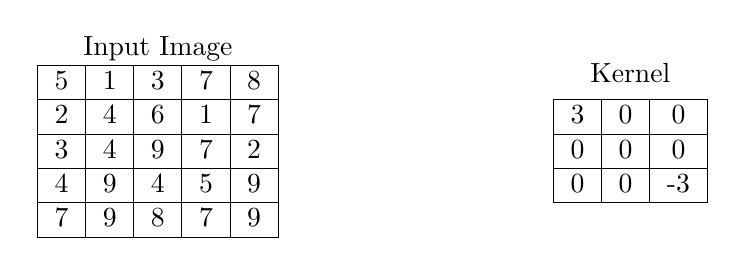
\begin{tikzpicture}
        \begin{scope}
            \node at (0,0) {
                \begin{tabular}{|c|c|c|c|c|}
                    \hline
                    5 & 1 & 3 & 7 & 8 \\
                    \hline
                    2 & 4 & 6 & 1 & 7 \\
                    \hline
                    3 & 4 & 9 & 7 & 2 \\
                    \hline
                    4 & 9 & 4 & 5 & 9 \\
                    \hline
                    7 & 9 & 8 & 7 & 9 \\
                    \hline
                \end{tabular}
            };
            \node at (0,1.3) {Input Image};
        \end{scope}
        \begin{scope}[xshift=6cm]
            \node at (0,0) {
                \begin{tabular}{|c|c|c|}
                    \hline
                    3 & 0 & 0 \\
                    \hline
                    0 & 0 & 0 \\
                    \hline
                    0 & 0 & -3 \\
                    \hline
                \end{tabular}
            };
            \node at (0,1) {Kernel};
        \end{scope}
    \end{tikzpicture}
\end{center}
Assume zero-padding with 1-pixel border is applied to the input image.\\
Estimate the output of convolving the input image with the kernel.\\
\vspace{2mm}
\textbf{Answer:}\\
The output matrix is obtained by applying the kernel to the input image matrix:
\begin{center}
    \textcolor{red}{
    \begin{tabular}{|c|c|c|c|c|}
        \hline
        12 & 18 & 3 & 21 & 0 \\
        \hline
        12 & 12 & 18 & -3 & -21 \\
        \hline
        27 & 6 & 3 & 9 & -3 \\
        \hline
        27 & 15 & 9 & 0 & -21 \\
        \hline
        0 & -12 & -27 & -12 & -15 \\
        \hline
    \end{tabular}
    }
\end{center}
\vspace{3mm}
\uline{\textbf{Problem 2}}\\
Suppose we have a Convolutional Neural Network (CNN) model with the following architecture:
\begin{itemize}
    \item Input Layer: Input Color Image of Size $128 \times 128 \times 3$.
    \item First Convolutional Layer: 5 Different Kernels of Size $3 \times 3 \times 3$ with a Stride of 5 and no zero padding.
    \item First Max-Pooling Layer: Pooling Size of $2 \times 2$.
    \item Second Convolutional Layer: 3 Different Kernels of Size $5 \times 5 \times 5$ with a Stride of 2 and no zero padding of size 2.
    \item $\ldots$
\end{itemize}
\textbf{Question 2.1:} What is the dimension of the output of the first Convolutional Layer and how many weights must be learned in the first Convolutional Layer (Assume any bias weights are not counted)?\\
\textbf{Answer:}\\
\begin{itemize}
    \item Dimension of the Output of the First Convolutional Layer: $\textcolor{red}{\underline{\underline{26 \times 26 \times 5}}}$\\
    \item Number of Weights to be Learned in the First Convolutional Layer: $\textcolor{red}{\underline{\underline{5 \times 3 \times 3 \times 3 = 135}}}$ weights\\
    (Weights in the Convolutional Layer are shared across all units in this layer).\\
\end{itemize}

\vspace{5mm}
\textbf{Question 2.2:} What is the main purpose of doing polling during training in a deep neural network? What is the dimension of the output of the first Max-Pooling Layer?\\
\textbf{Answer:}\\
\begin{itemize}
    \item The main purpose of doing pooling during training in a deep neural network is to \textcolor{red}{make sure that the subsequent layers of the CNNs can pick up larger-scale details}.\\
    \item Dimension of the Output of the First Max-Pooling Layer: $\textcolor{red}{\underline{\underline{13 \times 13 \times 5}}}$\\
\end{itemize}
\vspace{5mm}
\textbf{Question 2.3:} What is the dimension of the output of the second Convolutional Layer and how many weights must be learned in the second Convolutional Layer (Assume any bias weights are not counted)?\\
\textbf{Answer:}\\
\begin{itemize}
    \item Dimension of the Output of the Second Convolutional Layer: $\textcolor{red}{\underline{\underline{7 \times 7 \times 3}}}$\\
    \item Number of Weights to be Learned in the Second Convolutional Layer: $\textcolor{red}{\underline{\underline{3 \times 5 \times 5 \times 5 = 375}}}$ weights\\
    (Weights in the Convolutional Layer are shared across all units in this layer).\\
\end{itemize}

\chapter{Minimax and Alpha-Beta Pruning}
\textcolor{magenta}{\section{\textbf{Introduction to Games}}}
\textcolor{cyan}{\textbf{Games}} are a the oldest and most well-studied domain in Artificial Intelligence (AI) since they are \textcolor{violet}{fun}, \textcolor{violet}{easy to represent with a well-defined set of rules}, \textcolor{violet}{have a lot of possible combinations of moves}, \textcolor{violet}{involves strategy and planning}, and \textcolor{violet}{determines the programs' performance}.\\
There are 3 types of games:
\begin{enumerate}
    \item \textcolor{red}{Perfect and Imperfect Information Games}.
    \begin{itemize}
        \item \textcolor{cyan}{Perfect Information Games}: Games where both players \textcolor{violet}{know all the possible moves of both players and results}.
        \item \textcolor{cyan}{Imperfect Information Games}: Games where both players \textcolor{violet}{do not know all the possible moves of each other}.
    \end{itemize}
    \item \textcolor{red}{Zero Sum and Non-Zero Sum Games}.
    \begin{itemize}
        \item \textcolor{cyan}{Zero Sum Games}: 2-Player Games where the \textcolor{violet}{gain of one player is the loss of the other player}.
        \item \textcolor{cyan}{Non-Zero Sum Games}: 2-Player Games where the \textcolor{violet}{gain of one player is not necessarily the loss of the other player}.
    \end{itemize}
    \item \textcolor{red}{Deterministic and Non-Deterministic Games}.
    \begin{itemize}
        \item \textcolor{cyan}{Deterministic Games}: Games \textcolor{violet}{without random choices}.
        \item \textcolor{cyan}{Non-Deterministic Games}: Games where there are \textcolor{violet}{random choices}.
    \end{itemize}
\end{enumerate}
There is some games that has perfect information, zero-sum, and deterministic properties, one of them is Tic-Tac-Toe.\\
\vspace{2mm}
\uline{\large Tic-Tac-Toe}\\
\vspace{1mm}
\begin{wrapfigure}[8]{l}{0.15\textwidth}
    \centering
    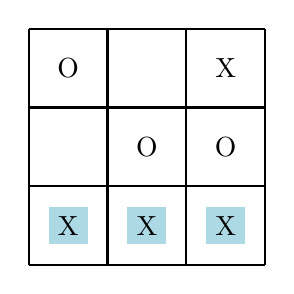
\begin{tikzpicture}
        \draw[thick] (0,0) grid (3,3);
        \node at (0.5,2.5) {O};
        \node at (1.5,2.5) {};
        \node at (2.5,2.5) {X};
        \node at (0.5,1.5) {};
        \node at (1.5,1.5) {O};
        \node at (2.5,1.5) {O};
        \node[fill=lightblue] at (0.5,0.5) {X};
        \node[fill=lightblue] at (1.5,0.5) {X};
        \node[fill=lightblue] at (2.5,0.5) {X};
    \end{tikzpicture}
\end{wrapfigure}
\textcolor{cyan}{Tic-Tac-Toe} is a paper-and-pencil game for two players, \textcolor{violet}{X} and \textcolor{violet}{O}, who take turns marking the spaces in a $3 \times 3$ grid.\\
The player who succeeds in placing three of their marks in a \textcolor{violet}{horizontal}, \textcolor{violet}{vertical}, or \textcolor{violet}{diagonal row} is the winner.\\
It has \textcolor{violet}{perfect information}, \textcolor{violet}{zero-sum}, and \textcolor{violet}{deterministic} properties.\\
\begin{itemize}
    \item Perfect Information: Both players know moves previously made.
    \item Zero-Sum: 2-Player Game with two outcomes Win/Loss or Draw.
    \\
    If Player 1 wins and scores 1, Player 2 loses and scores -1. If it is a draw, both players score 0.
    \item Deterministic: No random choices.
\end{itemize}
We will first try to use \textcolor{cyan}{Brute-Force Approach} to solve the game of Tic-Tac-Toe.\\
\textcolor{magenta}{\section{\textbf{AI Brute-Force/Naïve Approach}}}
\subsection{Rules of Brute-Force Approach}
Here are the rules of the Brute-Force Approach for general games:
\begin{itemize}
    \item First, If there is a \textcolor{cyan}{winning move for me}, make that move.
    \item Second, If the \textcolor{cyan}{opponent has a winning move}, block that move.
    \item Otherwise, make a \textcolor{cyan}{random move}.
\end{itemize}
However, the AI may not achieve the best possible outcome with this approach.\\
\newpage
\subsection{Brute-Force Approach for Tic-Tac-Toe}
At the beginning, a player can choose any of the 9 available empty spaces on the game board.\\
We represent these 9 available moves using a Tree Structure as shown below:\\
\begin{center}
    \begin{figure}[h]
        \centering
        \includegraphics[scale=0.25]{chapter 10/ch10_figure1.jpeg}
        \caption{Tic-Tac-Toe Game Tree}
    \end{figure}
\end{center}
Actions from the root node to the leaf nodes:
\begin{itemize}
    \item 1st Action: \textcolor{violet}{$9$ Possible Moves} at the beginning of the game.
    \item 2nd Action: \textcolor{violet}{$9 \times 8 = 72$ Possible Moves} (For each 9 moves, there are 8 possible moves).
    \item 3rd Action: \textcolor{violet}{$9 \times 8 \times 7 = 504$ Possible Moves}.
    \item 4th Action: \textcolor{violet}{$9 \times 8 \times 7 \times 6 = 3,024$ Possible Moves}.
    \item 5th Action: \textcolor{violet}{$9 \times 8 \times 7 \times 6 \times 5 = 15,120$ Possible Moves}.
    \item 6th Action: \textcolor{violet}{$9 \times 8 \times 7 \times 6 \times 5 \times 4 = 60,480$ Possible Moves}.
    \item 7th Action: \textcolor{violet}{$9 \times 8 \times 7 \times 6 \times 5 \times 4 \times 3 = 181,440$ Possible Moves}.
    \item 8th Action: \textcolor{violet}{$9 \times 8 \times 7 \times 6 \times 5 \times 4 \times 3 \times 2 = 362,880$ Possible Moves}.
    \item 9th Action: \textcolor{violet}{$9 \times 8 \times 7 \times \ldots \times 1 = 9! = 362,880$ Possible Moves}.
\end{itemize}
Enumerate all the possible states of the game:
\begin{align*}
    \text{Total Number of Possible States} &= 9 + 9 \times 8 + 9 \times 8 \times 7 + \ldots + 9 \times 8 \times 7 \times 6 \times 5 \times 4 \times 3 \times 2 \times 1\\
    &= \textcolor{red}{\underline{\underline{986,409}}}
\end{align*}
However, the game can end before there is no more empty space on the board, so the number of possible states is less than 986,409.\\
Instead, we want to determine which move to take based on the current state of the game by using the \textcolor{cyan}{Minimax Algorithm}.\\
\newpage
\textcolor{magenta}{\section{\textbf{Minimax Algorithm}}}
\subsection{Definition of Minimax Algorithm}
\begin{defBox}{Definition 10.3}{Minimax Algorithm}
    \raggedright
    The \textcolor{cyan}{Minimax Algorithm} is a \textcolor{red}{recursive algorithm} used to \textcolor{red}{choose an optimal move} for a player, assuming that the opponent is also playing optimally, which helps \textcolor{violet}{minimize that the other players can force us to receive}.\\
    \begin{itemize}
        \item Two players are \textcolor{cyan}{Maximizer (MAX)} and \textcolor{cyan}{Minimizer (MIN)} with a scoring method defined from the \textcolor{cyan}{standpoint of the MAX player}.
        \item The \textcolor{cyan}{Maximizer} tries to \textcolor{violet}{maximize the score} and the \textcolor{cyan}{Minimizer} tries to \textcolor{violet}{minimize the score}.
    \end{itemize}
\end{defBox}
Since the optimal play for maximizer is the worst-case scenario for the minimizer, \textcolor{cyan}{if the minimizer does not play optimally}, \textcolor{red}{the maximizer will do better}.\\
\subsection{Steps of Minimax Algorithm}
The Minimax Algorithm is implemented using the following steps:
\begin{enumerate}
    \item Construct a complete \textcolor{cyan}{Game Tree} to represent all possible moves.
    \item Apply the \textcolor{cyan}{Utility Function} to each terminal state of the tree to determine the \textcolor{violet}{numerical values(scores) of the game}.
    \item Beginning with the terminal states, \textcolor{cyan}{determine the utility of the predecessor nodes}:
    \begin{itemize}
        \item If the node is a \textcolor{cyan}{Maximizer Node}, \textcolor{violet}{choose the maximum value} of its children.
        \item If the node is a \textcolor{cyan}{Minimizer Node}, \textcolor{violet}{choose the minimum value} of its children.
    \end{itemize}
    \item From the initial state (Root of the Game Tree), the \textcolor{cyan}{Maximizer chooses the move with the maximum value} (Minimax Decision).\\
    \fbox{
        \parbox{0.92\textwidth}{
            Search the Game Tree in a \textcolor{cyan}{Depth-First-Search Manner} \textcolor{red}{(Algorithm for traversing/searching tree data structures)} to find the value of the root node.\\
            $\Rightarrow$ \textcolor{violet}{Starts at the root node and explores as far as possible along each branch before backtracking}.
        }
    }
\end{enumerate}
\uline{Example of Minimax Algorithm for Tic-Tac-Toe Game}\\
Consider the following Game Tree for a Tic-Tac-Toe Game with the following initial state:
\begin{itemize}
    \item Terminal States' Utility Values: Max Wins = 1, Max Loses = -1, Draw = 0.
    \item Maximizer is initialized to -$\infty$ and Minimizer is initialized to +$\infty$ for each node.
\end{itemize}
\begin{center}
    \includegraphics[scale=0.45]{chapter 10/ch10_figure2.png}
\end{center}
\newpage
\uwave{\textbf{Step 1:}}\\
For the leftmost state in level 2, the maximizer updates its value with the maximum of $-\infty$ and 0 where the value 0 is obtained from its child node in level 3.\\
The value of the maximizer is changed \textcolor{violet}{from $-\infty$ to 0}.\\
\vspace{3mm}
\uwave{\textbf{Step 2:}}\\
For the leftmost state in level 1, the minimizer updates its value with the minimum of $+\infty$ and 0 where the value 0 is obtained from its left child node in level 2.\\
The value of the minimizer is changed \textcolor{violet}{from $+\infty$ to 0}.\\
\vspace{3mm}
\uwave{\textbf{Step 3:}}\\
For the leftmost state in level 1, the minimizer updates its value with the minimum of 0 and -1 where the value -1 is obtained from its right child node in level 2.\\
The value of the minimizer is changed \textcolor{violet}{from 0 to -1}.\\
\vspace{3mm}
\uwave{\textbf{Step 4:}}\\
For the state in level 0, the maximizer updates its value with the maximum of $-\infty$ and -1 where the value -1 is obtained from its left child node in level 1.\\
The value of the maximizer is changed \textcolor{violet}{from $-\infty$ to -1}.\\
\vspace{3mm}
\uwave{\textbf{Step 5:}}\\
For the state in level 0, the maximizer updates its value with the maximum of -1 and +1 where the value +1 is obtained from its middle child node in level 1.\\
The value of the maximizer is changed \textcolor{violet}{from -1 to +1}.\\
\vspace{3mm}
\uwave{\textbf{Step 6:}}\\
For the state in level 2, the maximizer updates its value with the maximum of $-\infty$ and +1 where the value +1 is obtained from its child node in level 3.\\
The value of the maximizer is changed \textcolor{violet}{from $-\infty$ to +1}.\\
\vspace{3mm}
\uwave{\textbf{Step 7:}}\\
For the state in level 1, the minimizer updates its value with the minimum of $+\infty$ and +1 where the value +1 is obtained from its left child node in level 2.\\
The value of the minimizer is changed \textcolor{violet}{from $+\infty$ to +1}.\\
\vspace{3mm}
\uwave{\textbf{Step 8:}}\\
For the state in level 2, the maximizer updates its value with the maximum of $-\infty$ and 0 where the value 0 is obtained from its child node in level 3.\\
The value of the maximizer is changed \textcolor{violet}{from $-\infty$ to 0}.\\
\vspace{3mm}
\uwave{\textbf{Step 9:}}\\
For the state in level 1, the minimizer updates its value with the minimum of +1 and 0 where the value 0 is obtained from its right child node in level 2.\\
The value of the minimizer is changed \textcolor{violet}{from +1 to 0}.\\
\vspace{3mm}
\uwave{\textbf{Step 10:}}\\ 
For the state in level 0, the maximizer updates its value with the maximum of +1 and 0 where the value 0 is obtained from its right child node in level 1.\\
The value of the maximizer \textcolor{violet}{remains unchanged}.\\
\vspace{3mm}
\fbox{
    \parbox{0.97\textwidth}{
        \uwave{\textbf{Minimax Decision:}}
        \begin{itemize}
            \item In the top position, it is X's turn to play.
            \item If X plays in the top-center, then O can guarantee a win.
            \item If X plays in the left center, then X will win.
            \item If X plays in the right center, then O can force a draw.
        \end{itemize}
        \textcolor{red}{$\therefore$ The best move for X is to play in the left center}.
    }
}
\newpage
\textit{\large{Python Code Implementation of Minimax Algorithm for Tic-Tac-Toe Game:}}\\
\begin{lstlisting}[language=Python, basicstyle=\ttfamily\small, keywordstyle=\color{blue}, commentstyle=\color{forestgreen}, stringstyle=\color{red}, showstringspaces=false]
# Draw the current state of the game
def drawboard(board):
    print("Current state: \n\n")
    for i in range (0,9):
        if board[i] == 0:           # If value is 0, it's an empty cell
            print("- ",end = " ")
        if board[i] == 1:           # If value is 1, it's the mark of AI
            print("X ",end = " ")
        if board[i] == -1:          # If value is -1, it's the mark of human
            print("O ",end = " ")
        if (i+1) % 3 == 0:          # Move to the next line after printing 3 elements
            print("\n")
    print("\n")  # Move the next line after printing the game board

# Check if there is a player wins.
# If human player wins, return -1.
# If AI player wins, return 1.
# If draw, return 0.
# If the game is not finished, return 2.
def check_game(board):
    # There are 8 possible winning patterns.
    # 0, 1, 2 (1st row), 3, 4, 5 (2nd row), 6, 7, 8 (3rd row)
    # 0, 3, 6 (1st col), 1, 4, 7 (2nd col), 2, 5, 8 (3rd col)
    # 0, 4, 8 (Diagonal - top-left to bottom-right)
    # 2, 4, 6 (Diagonal - top-right to bottom-left)
    winning_pos = [ [0, 1, 2], [3, 4, 5], [6, 7, 8],
                    [0, 3, 6], [1, 4, 7], [2, 5, 8],
                    [0, 4, 8], [2, 4, 6] ]

    # Check all possible winning patterns for each player.
    for i in range(0,8):
        # Check whether the cell is non-empty AND the winning positions with the same mark
        if board[winning_pos[i][0]] != 0 and\
           board[winning_pos[i][0]] == board[winning_pos[i][1]] and\
           board[winning_pos[i][0]] == board[winning_pos[i][2]]:
           # Fulfiled the winning condition, return the mark of player
           return board[winning_pos[i][2]]

    # When reaching here, it means no player wins yet
    # Check whether there is an empty cell (i.e. with 0).
    # If so, the game is not finished. Return 2
    if any(element == 0 for element in board):
       return 2

    return 0  # Reach here, it means the game draws

# Obtain the user's input and update the board
def human_turn(board):
    pos = input("Enter O's position [1 to 9]: ")
    pos = int(pos) # Obtain user input, i.e., where to put the mark

    # If the cell picked by the human player is non-empty (i.e., non-zero), illegal
    if board[pos-1] != 0:
       print("Illegal Move!")
       exit(1)     # Terminate the program

    # When reaching here, the move is legal and we put -1 (put the mark of human player)
    board[pos-1] = -1
\end{lstlisting}
\newpage
\begin{lstlisting}[language=Python, basicstyle=\ttfamily\small, keywordstyle=\color{blue}, commentstyle=\color{forestgreen}, stringstyle=\color{red}, showstringspaces=false]
# Perform minimax search
def minimax(board, player):
    global count                # Refer to the global variable count in main
    count += 1                  # Make 1 call of minimax already
    result = check_game(board)  # Check if any player wins
    if result != 2:             # If the result is not 2, the game is finished,
       return result            # return 1 if the winner is AI,
                                # otherwise return -1 (i.e., human is the winner)

    scores = []                 # Create an empty list
    for i in range(0,9):        # Check all board locations
        if board[i] == 0:       # If the cell is empty
           board[i] = player    # Try to put the player's mark at cell i+1
           # Perform minimax for the next player, and append its score to the list
           scores.append(minimax(board,player*-1))
           board[i] = 0         # Undo the trial

    # Return the max score if the player is AI or return the min score if the player is human
    return max(scores) if player == 1 else min(scores)

# This function makes computer's move based on minimax.
def ai_turn(board):
    pos = -1         # Initialize pos to illegal value, -1, here
    max_value = -2   # Initialize max value so far to -2,
                     # which is a value smaller than the min value possible

    for i in range(0,9):
        if board[i] == 0:              # If the cell is empty
           board[i] = 1                # Try to put X at cell i+1
           score = minimax(board, -1)  # Calculate minimax score for the human player
           board[i] = 0                # Undo the trial
           if score > max_value:       # If we can a better score in the next level,
              max_value = score        # update the score and pos
              pos = i

    board[pos] = 1                     # Put X at pos, which is the best move


# Main function
# The broad is represented in a single dimensional list
# Initalize the board to all zeros (i.e., all empty cells)
board = [ 0, 0, 0, 0, 0, 0, 0, 0, 0 ]

print("Computer: X VS. You: O")
first = input("Play first (Y/N) :")
if first == 'Y' or first == 'y': # If first is 'Y'/'y', human wants to play first
   player = 1
else:
   player = 0

for i in range (0,9):            # Play the same. 9 turns in total
    if check_game(board) != 2:   # If the value returned by check\_game is not 2,
       break                     # the game is finished

    if (i+player) % 2 == 0:      # Take turns to play the game
       count = 0                 # Count the number of minimax calls
       ai_turn(board)
       print("Count:", count)    # Print the count
    else:
       drawboard(board)
       human_turn(board)

result = check_game(board)       # Check the game again
\end{lstlisting}
\newpage
\begin{lstlisting}[language=Python, basicstyle=\ttfamily\small, keywordstyle=\color{blue}, commentstyle=\color{forestgreen}, stringstyle=\color{red}, showstringspaces=false]
if result==0:                    # If the result is 0, draw
   drawboard(board)
   print("Draw!!!")
if result==1:                    # If the result is 1, AI wins
   drawboard(board)
   print("AI(X) Wins! Human(O) Loses!")
if result==-1:                   # If the result is -1, human wins
   drawboard(board)
   print("Human(O) Wins! AI(X) Loses!")

# Sample Output:

# Computer: X VS. You: O
# Play first (Y/N) :Y
# Current state: 
# 
# 
# -  -  -  
# 
# -  -  -  
# 
# -  -  -  
# 
# 
# 
# Enter O's position [1 to 9]: 1
# Count: 59704
# Current state: 
# 
# 
# O  -  -  
# 
# -  X  -  
# 
# -  -  -  
# 
# ...

# Draw!!!
\end{lstlisting}
\subsection{Disadvantages of Minimax Algorithm}
There are some disadvantages of the Minimax Algorithm:
\begin{itemize}
    \item \textcolor{red}{Huge Branching Factor}: Large Number of Children in Each Node makes the \textcolor{cyan}{process of reaching the goal state slow}.
    \item \textcolor{red}{Long Time} to \textcolor{cyan}{evaluate the entire game tree}.
    \item \textcolor{red}{Search and Evaluation of Unnecessary Nodes} in the Game Tree \textcolor{cyan}{degrades the overall performance and efficiency}.
    \item \textcolor{red}{Infeasible for Large Game Trees} with a large number of possible states for both min and max players.
    \item \textcolor{red}{Impossible to Explore the Entire Tree}: There is a \textcolor{cyan}{restriction of time and space}.
\end{itemize}
$\therefore$ We would like to use \textcolor{cyan}{Alpha-Beta Pruning} to find the optimal path in the game tree instead of doing all the possible moves in Minimax Algorithm.\\
\newpage
\textcolor{magenta}{\section{\textbf{Alpha-Beta Pruning}}}
\subsection{Definition of Alpha-Beta Pruning}
To \textcolor{violet}{prevent ourselves from exploring branches of the game tree that are not worth exploring}, we use the \textcolor{cyan}{Alpha-Beta Pruning Algorithm}.\\
\begin{defBox}{Definition 10.4}{Alpha-Beta Pruning}
    \raggedright
    We define two values \uuline{\textcolor{cyan}{Alpha ($\alpha$)} \textcolor{red}{= Best/Highest found so far along the  path for Max}} and \uuline{\textcolor{cyan}{Beta ($\beta$)} \textcolor{red}{= Best/Lowest found so far along the path for Min}} to store information about the potential of a branch for us or the opponent.\\
    \begin{itemize}
        \item \textcolor{cyan}{$\alpha$-Cutoff}: Terminate branch since \textcolor{violet}{AI has a better opportunity elsewhere already}.
        \item \textcolor{cyan}{$\beta$-Cutoff}: Terminate branch since \textcolor{violet}{Opponent has a better opportunity elsewhere already}.
    \end{itemize}
    We can \textcolor{cyan}{prune a branch} if \textcolor{red}{$\alpha \geq \beta$} since the \textcolor{violet}{opponent will never choose this branch}.\\
\end{defBox}
\subsection{Steps of Alpha-Beta Pruning}
The Alpha-Beta Pruning Algorithm is implemented using the following steps:
\begin{enumerate}
    \item We define two values \textcolor{cyan}{Alpha ($\alpha$)} and \textcolor{cyan}{Beta ($\beta$)} to store information about the potential of a branch for us or the opponent.\\
    $\Rightarrow$ $\alpha$ and $\beta$ are used to \textcolor{violet}{keep track of the curret upper and lower bounds}.
    \item Pass current values of $\alpha$ and $\beta$ of the parent node to the child nodes during the search.
    \item Update values of $\alpha$ and $\beta$ during the search:
    \begin{itemize}
        \item For \textcolor{cyan}{MAX}, compare $\alpha$ with the current node value (v).\\
        If \textcolor{cyan}{$\alpha < v$}, update \textcolor{red}{$\alpha = v$}. Otherwise, $\alpha$ remains unchanged.
        \item For \textcolor{cyan}{MIN}, compare $\beta$ with the current node value (v).\\
        If \textcolor{cyan}{$\beta > v$}, update \textcolor{red}{$\beta = v$}. Otherwise, $\beta$ remains unchanged.
    \end{itemize}
    \item Prune the remaining branches at the node if \textcolor{red}{$\alpha \geq \beta$}.
    \item Update the values of $\alpha$ and $\beta$ of the parent node using the values returned by the child nodes.
    \begin{itemize}
        \item If the parent node is a \textcolor{cyan}{MAX node}, compare $\alpha$ with the value of the child node (v).\\
        If \textcolor{cyan}{$\alpha < v$}, update \textcolor{red}{$\alpha = v$}. Otherwise, $\alpha$ remains unchanged.
        \item If the parent node is a \textcolor{cyan}{MIN node}, compare $\beta$ with the value of the child node (v).\\
        If \textcolor{cyan}{$\beta > v$}, update \textcolor{red}{$\beta = v$}. Otherwise, $\beta$ remains unchanged.
    \end{itemize}
\end{enumerate}
\uline{Example of Alpha-Beta Pruning Algorithm for Tic-Tac-Toe Game}\\
\uwave{\textbf{Step 1:}}\\
\begin{wrapfigure}[2]{r}{0.5\textwidth}
    \includegraphics[scale=0.1]{chapter 10/ch10_figure3.jpeg}
\end{wrapfigure}
The Max Player will initialize $\alpha$ to $-\infty$ and $\beta$ to $+\infty$.\\
Check whether $\alpha \geq \beta$: No, No Pruning is done.\\
\vspace{2cm}
\uwave{\textbf{Step 2:}}\\
The Max Player moves from the root node to its left child node by passing down the values of $\alpha = -\infty$ and $\beta = +\infty$.\\
\begin{wrapfigure}[4]{r}{0.37\textwidth}
    \includegraphics[scale=0.09]{chapter 10/ch10_figure4.jpeg}
\end{wrapfigure}
At the left node of the middle level, we do the following with the first terminal value 9:
\begin{itemize}
    \item Node Value = Min(Node Value, 9) = Min($\infty$, 9) = 9.
    \item $\beta$ = Min($+\beta$, 9) = Min($+\infty$, 9) = 9.
\end{itemize}
Check whether $\alpha \geq \beta$: No, No Pruning is done.\\
\vspace{1.2cm}
\uwave{\textbf{Step 3:}}\\
\begin{wrapfigure}[5]{r}{0.37\textwidth}
    \includegraphics[scale=0.09]{chapter 10/ch10_figure5.jpeg}
\end{wrapfigure}
The Max Player moves from the root node to its middle child.\\
At the left node of the middle level, we do the following with the second terminal value 8:
\begin{itemize}
    \item Node Value = Min(Node Value, 8) = Min(9, 8) = 8.
    \item $\beta$ = Min($+\beta$, 8) = Min(9, 8) = 8.
\end{itemize}
Check whether $\alpha \geq \beta$: No, No Pruning is done.\\
\newpage
\begin{wrapfigure}[6]{r}{0.37\textwidth}
    \includegraphics[scale=0.09]{chapter 10/ch10_figure6.jpeg}
\end{wrapfigure}
\uwave{\textbf{Step 4:}}\\
The Max Player moves from the root node to its right child.\\
At the left node of the middle level, we do the following with the second terminal value 7:
\begin{itemize}
    \item Node Value = Min(Node Value, 7) = Min(8, 7) = 7.
    \item $\beta$ = Min($+\beta$, 7) = Min(8, 7) = 7.
\end{itemize}
Check whether $\alpha \geq \beta$: No, No Pruning is done.\\
\vspace{1mm}
\uwave{\textbf{Step 5:}}\\
The algorithm backtracks to the root node, where the value 7 of the middle left node is passed to the parent node.\\
\begin{wrapfigure}[4]{r}{0.37\textwidth}
    \includegraphics[scale=0.09]{chapter 10/ch10_figure7.jpeg}
\end{wrapfigure}
At the root node, we do the following with the returned value 7:
\begin{itemize}
    \item Node Value = Max(Node Value, 7) = Max($-\infty$, 7) = 7.
    \item $\alpha$ = Max($\alpha$, 7) = Max($-\infty$, 7) = 7.
\end{itemize}
Check whether $\alpha \geq \beta$: No, No Pruning is done.\\
\vspace{1.2cm}
\uwave{\textbf{Step 6:}}\\
The Max Player moves from the root node to its middle child passing down the values of $\alpha = 7$ and $\beta = +\infty$.\\
\begin{wrapfigure}[4]{r}{0.35\textwidth}
    \includegraphics[scale=0.09]{chapter 10/ch10_figure8.jpeg}
\end{wrapfigure}
At the middle node of the middle level, we do the following with the first terminal value 6:
\begin{itemize}
    \item Node Value = Min(Node Value, 6) = Min($\infty$, 6) = 6.
    \item $\beta$ = Min($+\beta$, 6) = Min($+\infty$, 6) = 6.
\end{itemize}
Check whether $\alpha \geq \beta$:Yes, Pruning is done since $\alpha = 7$ is greater than $\beta = 6$.\\
\vspace{1.2cm}
\uwave{\textbf{Step 7:}}\\
The algorithm backtracks to the root node, where the value 6 of the center node of the middle layer is passed to the parent node.\\
\begin{wrapfigure}[4]{r}{0.35\textwidth}
    \includegraphics[scale=0.09]{chapter 10/ch10_figure9.jpeg}
\end{wrapfigure}
At the root node, we do the following with the returned value 6:
\begin{itemize}
    \item Node Value = Max(Node Value, 6) = Max(7, 6) = 7.
    \item $\alpha$ = Max($\alpha$, 7) = Max(7, 6) = 7.
\end{itemize}
Check whether $\alpha \geq \beta$: No, No Pruning is done.\\
\vspace{1.2cm}
\uwave{\textbf{Step 8:}}\\
The Max Player moves from the root node to its right child passing down the values of $\alpha = 7$ and $\beta = +\infty$.\\
\begin{wrapfigure}[4]{r}{0.35\textwidth}
    \includegraphics[scale=0.09]{chapter 10/ch10_figure10.jpeg}
\end{wrapfigure}
At the right node of the middle level, we do the following with the first terminal value 3:
\begin{itemize}
    \item Node Value = Min(Node Value, 3) = Min($\infty$, 3) = 3.
    \item $\beta$ = Min($+\beta$, 3) = Min($+\infty$, 3) = 3.
\end{itemize}
Check whether $\alpha \geq \beta$: Yes, Pruning is done since $\alpha = 7$ is greater than $\beta = 3$.\\
\vspace{1.2cm}
\uwave{\textbf{Step 9:}}\\
The algorithm backtracks to the root node, where the value 3 of the right node of the middle layer is passed to the parent node.\\
\begin{wrapfigure}[4]{r}{0.35\textwidth}
    \includegraphics[scale=0.09]{chapter 10/ch10_figure11.jpeg}
\end{wrapfigure}
At the root node, we do the following with the returned value 3:
\begin{itemize}
    \item Node Value = Max(Node Value, 3) = Max(7, 3) = 7.
    \item $\alpha$ = Max($\alpha$, 3) = Max(7, 3) = 7.
\end{itemize}
Check whether $\alpha \geq \beta$: No, No Pruning is done.\\
\vspace{1.5cm}
\fbox{
    \parbox{0.97\textwidth}{
        \uwave{\textbf{Alpha-Beta Pruning Decision:}}
        \begin{itemize}
            \item The best value for the root node is \textcolor{red}{7}.
        \end{itemize}
        \begin{center}
            \includegraphics[scale=0.09]{chapter 10/ch10_figure12.jpeg}
        \end{center}
    }
}
\newpage
\textit{\large{Python Code Implementation of Alpha-Beta Pruning for Tic-Tac-Toe Game:}}\\
\begin{lstlisting}[language=Python, basicstyle=\ttfamily\small, keywordstyle=\color{blue}, commentstyle=\color{forestgreen}, stringstyle=\color{red}, showstringspaces=false]
# Draw the current state of the game
def drawboard(board):
    print("Current state: \n\n")
    for i in range (0,9):
        if board[i] == 0:           # If value is 0, it's an empty cell
            print("- ",end = " ")
        if board[i] == 1:           # If value is 1, it's a mark of AI
            print("X ",end = " ")
        if board[i] == -1:          # If value is -1, it's a mark of the human
            print("O ",end = " ")
        if (i+1) % 3 == 0:          # Move to the next line after printing 3 elements
            print("\n")
    print("\n")  # Move the next line after printing the game board

# Check if there is a player wins.
# If human player wins, return -1.
# If AI player wins, return 1.
# If draw, return 0.
# If the game is not finished, return 2.
def check_game(board):
    # There are 8 possible winning patterns.
    # 0, 1, 2 (1st row), 3, 4, 5 (2nd row), 6, 7, 8 (3rd row)
    # 0, 3, 6 (1st col), 1, 4, 7 (2nd col), 2, 5, 8 (3rd col)
    # 0, 4, 8 (Diagonal - top-left to bottom-right)
    # 2, 4, 6 (Diagonal - top-right to bottom-left)
    winning_pos = [ [0, 1, 2], [3, 4, 5], [6, 7, 8],
                    [0, 3, 6], [1, 4, 7], [2, 5, 8],
                    [0, 4, 8], [2, 4, 6] ]

    # Check all possible winning patterns for each player.
    for i in range(0,8):
        # Check whether the cell is non-empty AND the winning positions with the same mark
        if board[winning_pos[i][0]] != 0 and\
            board[winning_pos[i][0]] == board[winning_pos[i][1]] and\
            board[winning_pos[i][0]] == board[winning_pos[i][2]]:
            # Fulfiled the winning condition, return the mark of player
            return board[winning_pos[i][2]]

    # When reaching here, it means no player wins yet
    # Check whether there is an empty cell (i.e. with 0)
    # If so, the game is not finished. Return 2
    if any(element == 0 for element in board):
        return 2

    return 0  # Reach here, it means the game draws

# Obtain the user's input and update the board
def human_turn(board):
    pos = input("Enter O's position [1 to 9]: ")
    pos = int(pos)  # Obtain user input, i.e., where to put the mark

    # If the cell picked by the human player is non-empty (i.e., non-zero), illegal
    if board[pos-1] != 0:
        print("Illegal Move!")
        exit(1)      # Terminate the program

    # When reaching here, the move is legal and we put -1 (put the mark of human player)
    board[pos-1] = -1
\end{lstlisting}
\newpage
\begin{lstlisting}[language=Python, basicstyle=\ttfamily\small, keywordstyle=\color{blue}, commentstyle=\color{forestgreen}, stringstyle=\color{red}, showstringspaces=false]
# Perform minimax search with alpha-beta pruning
def minimax_abp(board, player, alpha = -float('inf'), beta = float('inf')):
    global count                # Refer to the global variable count in main
    count += 1                  # Make 1 call of minimax_abp already
    result = check_game(board)  # Check if any player wins
    if result != 2:             # If the result is not 2, the game is finished,
        return result           # return 1 if the winner is AI,
                                # otherwise return -1 (i.e., human is the winner)
    if player == 1:
        value = -float('inf')
        for i in range(0,9):               # Check all board locations
            if board[i] == 0:              # If the cell is empty
                board[i] = player          # Try to put the player's mark at cell i+1
                # Perform minimax with alpha-beta pruning for the next player
                # and update current value if needed
                value = max(value, minimax_abp(board, player*-1, alpha, beta))
                alpha = max(alpha, value)  # Update alpha with max of current alpha and value
                board[i] = 0               # Undo the trial
                if alpha >= beta: break
    else:
        value = float('inf')
        for i in range(0,9):               # Check all board locations
            if board[i] == 0:              # If the cell is empty
                board[i] = player          # Try to put the player's mark at cell i+1
                # Perform minimax with alpha-beta pruning for the next player
                # and update current value if needed
                value = min(value, minimax_abp(board, player*-1, alpha, beta))
                beta = min(beta, value)    # Update beta with min of current beta and value
                board[i] = 0               # Undo the trial
                if alpha >= beta: break

    # Return the max score if the player is AI or return the min score if the player is human
    return value

# This function makes computer's move based on minimax.
def ai_turn(board):
    pos = -1         # Initialize pos to illegal value, -1, here
    max_value = -2   # Initialize max value so far to -2,
                        # which is a value smaller than the min value possible

    for i in range(0,9):
        if board[i] == 0:                   # If the cell is empty
            board[i] = 1                    # Try to put X at cell i+1
            score = minimax_abp(board, -1)  # Calculate minimax score for the human player
            board[i] = 0                    # Undo the trial
            if score > max_value:           # If we can a better score in the next level,
                max_value = score           # update the score and pos
                pos = i

    board[pos] = 1                          # Put X at pos, which is the best move
\end{lstlisting}
\newpage
\begin{lstlisting}[language=Python, basicstyle=\ttfamily\small, keywordstyle=\color{blue}, commentstyle=\color{forestgreen}, stringstyle=\color{red}, showstringspaces=false]
# Main function

# The broad is represented in a single dimensional list
# Initalize the board to all zeros (i.e., all empty cells)
board = [ 0, 0, 0, 0, 0, 0, 0, 0, 0 ]

print("Computer: X VS. You: O")
first = input("Play first (Y/N) :")
if first == 'Y' or first == 'y': # If first is 'Y'/'y', human wants to play first
    player = 1
else:
    player = 0

for i in range (0,9):           # Play the same. 9 turns in total
    if check_game(board) != 2:  # If the value returned by check_win is not 2, the game is finished
        break
    if (i+player) % 2 == 0:     # Take turns to play the game
        count = 0               # Count the number of minimax_abp calls
        ai_turn(board)
        print("Count:", count)  # Print the count
    else:
        drawboard(board)
        human_turn(board)

result = check_game(board)      # Check the game again

if result==0:                   # If the result is 0, draw
    drawboard(board)
    print("Draw!!!")
if result==1:                   # If the result is 1, AI wins
    drawboard(board)
    print("AI(X) Wins! Human(O) Loses!")
if result==-1:                  # If the result is -1, human wins
    drawboard(board)
    print("Human(O) Wins! AI(X) Loses!")

# Sample Output:

# Computer: X VS. You: O
# Play first (Y/N) :Y
# Current state:
#
# -  -  -
#
# -  -  -
#
# -  -  -
#
#
#
# Enter O's position [1 to 9]: 1
# Count: 4089
# Current state:
#
# O  -  -
#
# -  X  -
#
# -  -  -
#
# ...
#
# AI(X) Wins! Human(O) Loses!
\end{lstlisting}
\newpage
\subsection{Advantages and Disadvantages of Alpha-Beta Pruning}
There are some advantages of the Alpha-Beta Pruning Algorithm:
\begin{itemize}
    \item \textcolor{cyan}{Reduces the number of nodes} to be evaluated in the Minimax Algorithm.
    \item \textcolor{cyan}{Stops assessing a move} when at least one option has been found that proves the move to be at the minmimum.
    \item \textcolor{cyan}{Improves the search efficiency} by \textcolor{violet}{pruning branches} of the game tree that need not be searched.
\end{itemize}
However, there are some disadvantages of the Alpha-Beta Pruning Algorithm:
\begin{itemize}
    \item \textcolor{cyan}{Still needs to search all the way to terminal states} although it may prune large parts of the search tree.
    \item \textcolor{cyan}{Moves must be made in reasonable time} to be effective for some games.
\end{itemize}
To solve the disadvantages of the Alpha-Beta Pruning Algorithm, we can \textcolor{cyan}{set a depth limit} to the search tree or use \textcolor{cyan}{Heruistic Evaluation Functions} (Estimated Desirability/Utility of Position) to \textcolor{red}{correlate with the actual chance of winning}.\\
$\therefore$ The \textcolor{cyan}{Alpha-Beta Pruning Algorithm} is a \textcolor{violet}{more efficient} and \textcolor{violet}{effective} algorithm for \textcolor{violet}{searching game trees} than the Minimax Algorithm.\\
\vfill
\textbf{\textcolor{purple}{\Large{Practice Problem}}}\\
Consider the game tree below filled with the values returned by the standard Minimax Algorithm.\\
\begin{center}
    \includegraphics[scale=0.2]{chapter 10/ch10_figure13.jpeg}
\end{center}
\textbf{Question 1:} State the best initial move for the first player (E-1 or E-2).
\textbf{Answer:} The best initial move for the first player is \textcolor{red}{E-1}.\\
\vspace{3mm}
\textbf{Question 2:} Apply the Alpha-Beta Pruning Algorithm to the game tree and state the branches that need not be examined or considered by putting down the edge labels.\\
\textbf{Answer:} The branches that need not be examined or considered are as follows:
\begin{itemize}
    \item \textcolor{red}{E-18}
    \item \textcolor{red}{E-22}
    \item \textcolor{red}{E-26}
    \item \textcolor{red}{E-28}
    \item \textcolor{red}{E-30}
\end{itemize}

\chapter{Ethics of Artificial Intelligence}
\textcolor{magenta}{\section{\textbf{Definition of AI Ethics}}}
AI Ethics means the \textcolor{violet}{ethical issues surrounding the use of Artificial Intelligence (AI) technologies}.\\
There is a more formal definition of AI Ethics defined by the \textcolor{cyan}{UK's Alan Turing Institute} as follows:
\begin{defBox}{Definition 11.1}{AI Ethics}
    \textcolor{cyan}{AI Ethics} is the \textcolor{red}{set of values, principles, and techniques} that employ widely accepted \textcolor{red}{standards of right and wrong} to guide the development and deployment of AI technologies.
\end{defBox}
In practice, it means that \textcolor{cyan}{organizations using AI} including the globe, governments, industry groups and others, should have the \textcolor{violet}{right AI ethics policy} and \textcolor{violet}{governance practices} to ensure the \textcolor{red}{technology is used for good} and \textcolor{red}{not for harm unintentionally}.\\
\vspace{3mm}
There are some \textcolor{violet}{potential harms} that can be caused by the AI Systems:
\begin{itemize}
    \item \textcolor{cyan}{Invading people's right to privacy}: AI may processes the data without consent or handling it in a way that reveals personal information without an individual's permission.
    \item \textcolor{cyan}{Unfairness}: AI may \textcolor{violet}{make biased/unfair decisions/recommendations} about certain populations or demographics.
    \item \textcolor{cyan}{Making decisions that cannot be explained in plain language}: It is unclear if AI's conclusions are fair and unbiased.
    \item \textcolor{cyan}{Unreliaibility}: AI may \textcolor{violet}{make unreliable decisions or delivering poor quality outcomes} due to model implementation or data quality issues.
    \item \textcolor{cyan}{Denying people's rights}: AI may \textcolor{violet}{deny people's rights to account for decisions} made by AI systems about them.
\end{itemize}
To understand these potential harms, we need to understand the \textcolor{violet}{ethical issues surrounding AI} and the \textcolor{violet}{ethical principles} that should be followed when developing and deploying AI technologies.\\
\textcolor{magenta}{\section{\textbf{AI Ethics Issues}}}
AI technology is neither ethical nor unethical. Instead, \textcolor{violet}{principles or frameworks} must be established by \textcolor{cyan}{enterprises} to ensure that they use the AI systems ethically and responsibly for guarding against AI misuse.\\
However, there are some problems existing for the principles or frameworks established by enterprises:
\begin{itemize}
    \item \textcolor{red}{Non-consensus}: There is \textcolor{violet}{no consensus} about what \textcolor{violet}{ethical responsibilities} enterprises have for different AI applications.
    \item \textcolor{red}{Different Interpretations}: Different AI-focused executives can look at the same AI application and \textcolor{violet}{interpret the ethical responsibilities differently}.
\end{itemize}
There are a lot of \textcolor{cyan}{ethical dilemmas} that can arise from the use of AI technologies, ranging from \textcolor{violet}{deciding whose lives autonomous vehicles should prioritize saving in a multi-person crash situation} to \textcolor{violet}{ensuring that credit scoring AIs do not discriminate against certain populations unfairly}.\\
\vspace{2mm}
This makes the general public and business community become increasingly aware of the ethical issues surrounding AI uses.\\
Generally, there are \textcolor{red}{three main areas of AI Ethics Issues} to ensure the AI models in production in their organizations are \textcolor{violet}{function ethically and responsibly}:
\begin{enumerate}
    \item \textcolor{cyan}{Data Ethics}
    \item \textcolor{cyan}{AI Model Bias}
    \item \textcolor{cyan}{AI Model Monitoring and Maintenance}
\end{enumerate}
\newpage
\subsection{Data Ethics}
\begin{defBox}{Definition 11.2.1}{Data Ethics}
    \textcolor{cyan}{Data Ethics} is the branch of ethics that ensures \textcolor{red}{AI models function in a way that is fair, unbiased and in customers' best interests}, starting with ensuring data that feeds into them is collected, governed and used ethically.
\end{defBox}
It ensures companies secure the \textcolor{violet}{proper consent from customers} before using their data and handle it in a secure way \textcolor{violet}{respecting their privacy}.\\
Moreover, it takes proactive steps to address data bias in those datasets and ensure the \textcolor{violet}{populatioons being analyzed are fairly represented} in the data.\\
\subsection{AI Model Bias}
\begin{defBox}{Definition 11.2.2}{AI Model Bias}
    \textcolor{cyan}{AI Model Bias} is to ensure that \textcolor{red}{data that feeds AI models is relatively unbiased}.
\end{defBox}
AI and ML ethics require enterprises to ensure that those AI and ML models are built to \textcolor{violet}{ensure their decisions made are fair and unbiased}.\\
\subsection{AI Model Monitoring and Maintenance}
\begin{defBox}{Definition 11.2.3}{AI Model Monitoring and Maintenance}
    \textcolor{cyan}{AI Model Monitoring and Maintenance} means some \textcolor{red}{ML models adjust themselves to improve their accuracy over time}.
\end{defBox}
\textcolor{cyan}{AI Model Drift} Phenomenon will happen if others see their accuracy change over time due to the changes in the data flowing into them.\\
Enterprises must \textcolor{violet}{ensure AI models are effectively monitored} and \textcolor{violet}{maintained to continue functioning as intended} over time.\\
\textcolor{magenta}{\section{\textbf{Ethical Principles for AI}}}
A number of \textcolor{cyan}{ethical principles} have been proposed to guide the development and deployment of AI technologies by organizations.\\
One of the Most Commonly Used Ethical Principles is the \textcolor{cyan}{Seven European Union Principles for AI}.\\
\vspace{2mm}
\subsection{Seven European Union Principles for AI}
\begin{enumerate}
    \item \textcolor{cyan}{Human Agency and Oversight}: AI should \textcolor{violet}{empower human beings} and \textcolor{violet}{allow them to make informed decisions}.
    \item \textcolor{cyan}{Technical Robustness and Safety}: AI should be \textcolor{violet}{resilient and secure}. They need to be \textcolor{violet}{safe ensuring a fall-back plan in case of problems}.
    \item \textcolor{cyan}{Privacy and Data Governance}: AI should \textcolor{violet}{ensure adequate data governance mechanisms} to \textcolor{violet}{protect privacy and confidentiality}.
    \item \textcolor{cyan}{Transparency}: AI should be \textcolor{violet}{transparent and traceable}. The data, system and AI business models should be \textcolor{violet}{explainable}.
    \item \textcolor{cyan}{Diversity, Non-discrimination and Fairness}: AI should \textcolor{violet}{ensure diversity, non-discrimination and fairness}. The AI systems should be \textcolor{violet}{unbiased and provide equal opportunities}.
    \item \textcolor{cyan}{Societal and Environmental Well-being}: AI should be \textcolor{violet}{used to enhance societal and environmental well-being}. The AI systems should be \textcolor{violet}{sustainable and environmentally friendly}.
    \item \textcolor{cyan}{Accountability}: AI should be \textcolor{violet}{accountable and transparent}. The AI systems should be \textcolor{violet}{auditable and have clear responsibilities}.
\end{enumerate}
\subsection{Common Grounds for Ethical Principles}
There are many lists of principles, but they can be synthesized into five fundamental principles:
\begin{enumerate}
    \item \textcolor{red}{\hl{Autonomy}}: People should be able to make their own decisions.
    \item \textcolor{red}{\hl{Beneficence}}: Society at large should benefit.
    \item \textcolor{red}{\hl{Non-maleficence}}: Harmful consequences should be avoided.
    \item \textcolor{red}{\hl{Justice}}: Diversity, Non-discrimination and Fairness should be ensured.
    \item \textcolor{red}{\hl{Explicability}}: Transparency and Explainability should be ensured.
\end{enumerate}
\subsection{Problems with Ethical Principles}
There are some problems with the ethical principles since they are very high-level and abstract:
\begin{itemize}
    \item \textcolor{violet}{Interpreted in Different Ways}.
    \item \textcolor{violet}{Conflict with Each Other in Concrete Cases}.
    \item \textcolor{violet}{Conflict in Practice}.
\end{itemize}
\fbox{
    \parbox{0.97\textwidth}{
        However, it is good to have these principles as \textcolor{cyan}{orientation points and evaluate solutions}.
    }
}
\newpage
\textcolor{magenta}{\section{\textbf{Fairness in AI}}}
Enforing fairness is important especially in ML because \textcolor{cyan}{many things have become automated by machines} and \textcolor{cyan}{groups and individuals may suffer if AI systems are not fair}.\\
There are some examples of unfairness in AI:
\begin{itemize}
    \item Face recognition in Google Photo mis-classifiers African Americans as gorillas.
    \item A search query in XING orders less qualified male candidates higher than more qualified female candidates.
\end{itemize}
Here are some of the reasons why AI systems can be unfair:
\begin{itemize}
    \item \textcolor{cyan}{\hl Skewed Sample}: If some initial bias happens, the bias may compound over time.:\\
    Future observations confirm prediction and fewer opportunities to make observations that contradict the prediction.
    \item \textcolor{cyan}{\hl Tainted Examples}: If the training data is not representative, the model will not be fair.
    \item \textcolor{cyan}{\hl Limited Data}: Some features may be less informative for some groups.
    \item \textcolor{cyan}{\hl Sample Size Disparity}: Training data from a minority group may be too small.
\end{itemize}
\textcolor{magenta}{\section{\textbf{Moral Decisions in AI}}}
There are some properties for machines to act morally even though philosophers consider machines are not capable of moral decisions:
\begin{itemize}
    \item Beliefs about the world.
    \item Pro-Attributes.
    \item Moral Knowledge.
    \item Possibility to compute what consequences actions have.
\end{itemize}
\uline{Example of Moral Decisions in AI:}\\
If a self-driving car has to decide between hitting a pedestrian or a wall, it has to make a moral decision. However, the car has a faster reaction time than a human and can compute the consequences of its actions to make a decision.\\
\vfill
\textbf{\textcolor{purple}{\Large{Practice Problem}}}\\
\textbf{Question:}\\
Match the European Union Principles with the Given Common Grounds by Completing the Following Table with the Corresponding Numbers.\\
\begin{center}
    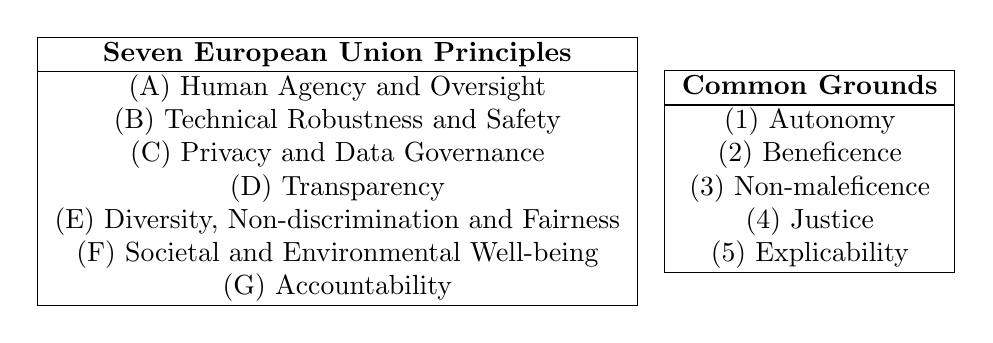
\begin{tikzpicture}
        \begin{scope}
            \node at (0,0){
                \begin{tabular}
                    {|c|}
                    \hline
                    \textbf{Seven European Union Principles} \\
                    \hline
                    (A) Human Agency and Oversight \\
                    (B) Technical Robustness and Safety \\
                    (C) Privacy and Data Governance \\
                    (D) Transparency \\
                    (E) Diversity, Non-discrimination and Fairness \\
                    (F) Societal and Environmental Well-being \\
                    (G) Accountability \\ 
                    \hline
                \end{tabular}
            };
        \end{scope}
        \begin{scope}
            \node at (6,0){
                \begin{tabular}
                    {|c|}
                    \hline
                    \textbf{Common Grounds} \\
                    \hline
                    (1) Autonomy \\
                    (2) Beneficence \\
                    (3) Non-maleficence \\
                    (4) Justice \\
                    (5) Explicability \\
                    \hline
                \end{tabular}
            };
        \end{scope}
    \end{tikzpicture}
\end{center}

\textbf{Answer:}\\
\begin{center}
    \begin{tabular}
        {|c|c|c|c|c|c|c|}
        \hline
        A & B & C & D & E & F & G \\
        \hline
        \textcolor{red}{5} & \textcolor{red}{3} & \textcolor{red}{1} & \textcolor{red}{5} & \textcolor{red}{4} & \textcolor{red}{2} & \textcolor{red}{1} \\
        \hline
    \end{tabular}
\end{center}


\end{document}
